\chapter{Analysis and Discussion}

This chapter provides analysis for both agent training and trained agent performance phases of the simulation experiments. For agent training, this will include the comparison of final and highest MACR100 scores for the different simulation experiments. Explanations are offered where an agent performance is poor. Similarly, a comparison of trained agent performance from the different experiments is provided, as well as a comparison to an optimally trained PI controller. Explanations are offered for instances where trained agent performance does not exceed the tuned PI controller.

\section{Training}
Monotonically increasing cumulative reward values indicate a continuous average increase in deep reinforcement learning agent performance. This is a desirable feature for cumulative reward plots. Plots of the MACR100 evolution for each experiment are detailed in Figures \ref{fig:6201_average_reward}, \ref{fig:6301_average_reward}, \ref{fig:6401_average_reward}, \ref{fig:6501_average_reward}, \ref{fig:6601_average_reward}, \ref{fig:6701_average_reward}, and \ref{fig:6801_average_reward}.

Generally, it can be observed that MACR100 is positively correlated with the episode number for all experiments. It is noted that the MACR100 signals were not monotonic for any experiment. Moreover, the MACR100 plots feature small to large fluctuations in the signal with increase in episode. This is especially true for the neural network experiment, expert learner experiment, and stochastic load demand experiment.

During the early stages of training all experiments demonstrated a period during which rapid learning took place. This is indicated by a steep rise in the MACR100 score, which typically took place in the first 1000 episodes of training, as shown in Figure \ref{fig:7101_MACR100_first}. In all experiments the agents demonstrated policy convergence, as indicated in reduced fluctuations of the MACR100 score. Convergence typically took place after the episode 7000, as shown in Figure \ref{fig:7102_MACR100_second}.

\clearpage

\begin{figure}[h]
	\centering
	
	% This file was created by tikzplotlib v0.9.1.
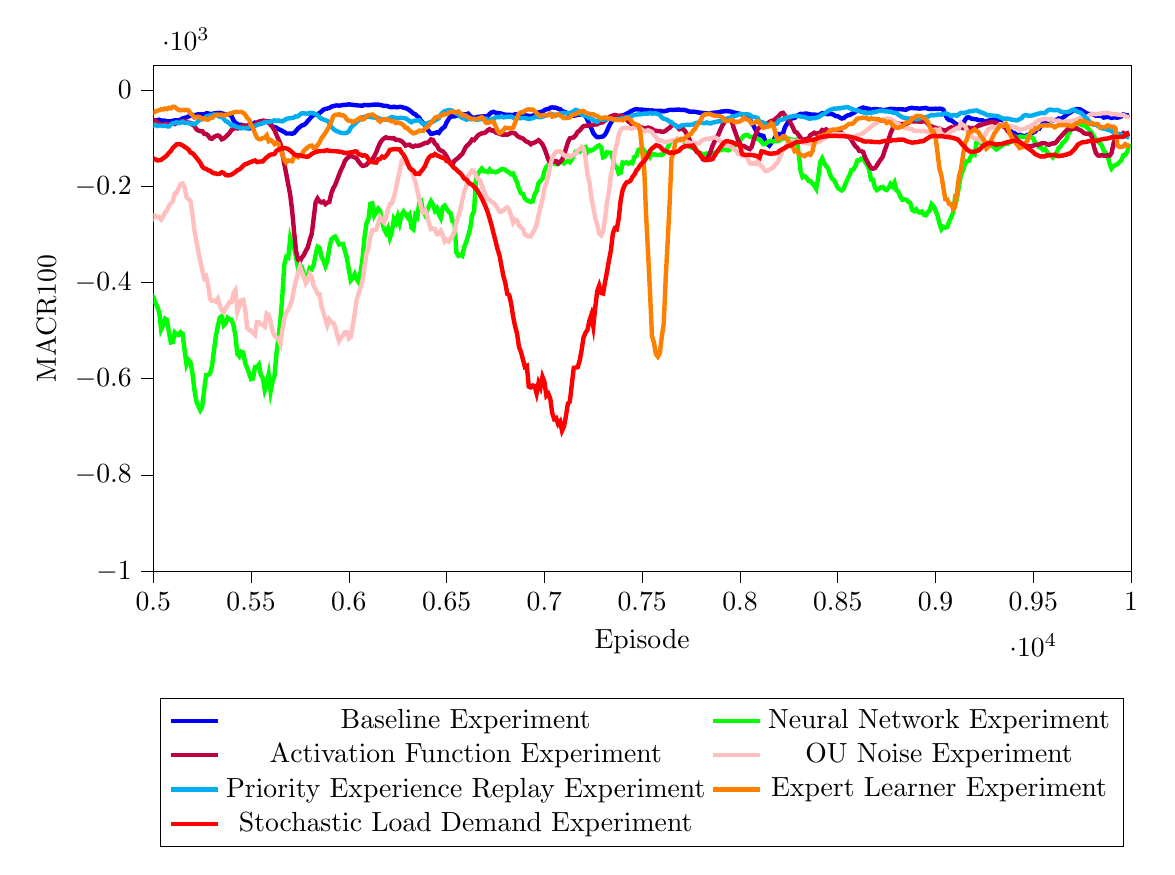
\begin{tikzpicture}

\definecolor{color0}{rgb}{1,0.498039215686275,0.0549019607843137}
\definecolor{color1}{rgb}{0.12156862745098,0.466666666666667,0.705882352941177}

\begin{axis}[
compat=newest,
tick align=outside,
tick pos=left,
x grid style={white!69.0196078431373!black},
xmin=5000, xmax=10000,
xtick style={color=black},
y grid style={white!69.0196078431373!black},
ymin=-1000.00, ymax=50.00,
ytick style={color=black},
scaled y ticks=true,
scaled y ticks=base 10:-3,
width=14cm,
height=8cm,
xlabel=Episode,
ylabel=MACR100,
%y label style={at={(-0.2,0.5)}}
%legend pos=south east
legend columns=2,
legend style={at={(0.5,-0.25)},anchor=north}
]

\addplot [ultra thick, blue]
table {%
100 -1582.67067718997
110 -1683.01661596282
120 -1790.32405198101
130 -1719.45505368521
140 -1626.98913277438
150 -1565.74285100258
160 -1418.63315026896
170 -1371.80179916204
180 -1375.93924454321
190 -1345.46802417995
200 -1298.37396567856
210 -1193.14672097731
220 -1139.18974455561
230 -1168.83869968173
240 -1172.51147639978
250 -1168.13326544273
260 -1245.39875298235
270 -1303.16914844481
280 -1324.62036687109
290 -1354.06203288941
300 -1389.75254102123
310 -1393.8006463874
320 -1355.15305241583
330 -1311.11801617452
340 -1283.81636104541
350 -1219.64857747229
360 -1189.39125920986
370 -1113.86327240352
380 -1062.58838313853
390 -1031.85292795208
400 -958.144683185093
410 -903.117037009552
420 -871.626221316283
430 -831.302898389944
440 -763.841713296356
450 -724.794912013634
460 -659.416291918026
470 -609.688945607528
480 -549.865720029054
490 -476.247230741856
500 -437.928122162497
510 -421.569590654568
520 -411.202150282573
530 -388.304445701138
540 -374.749589238142
550 -362.886271385558
560 -347.596375581264
570 -359.99439814117
580 -344.471662650798
590 -342.856988696357
600 -342.609112249219
610 -336.306884815506
620 -338.623330229533
630 -321.162498138758
640 -301.841472871826
650 -290.037860479904
660 -299.222975781901
670 -305.734249260761
680 -287.272937068945
690 -273.380943968795
700 -262.731331361897
710 -237.221636611637
720 -215.288745999989
730 -227.27084028216
740 -235.426467129444
750 -258.290633844516
760 -289.037785015782
770 -256.019760645466
780 -254.985715886778
790 -254.544580722355
800 -262.352660976914
810 -268.927054447971
820 -267.3622969706
830 -270.41158495355
840 -278.076802614562
850 -270.538887467588
860 -227.752489432417
870 -244.934563245234
880 -267.372165644971
890 -280.525712729855
900 -278.457870859474
910 -274.41286096963
920 -305.858625936095
930 -319.593726469206
940 -342.036494103142
950 -370.369579555932
960 -367.93461225045
970 -386.126320813181
980 -414.995185456001
990 -430.932935656827
1000 -466.023097142712
1010 -495.411388378483
1020 -495.274861982452
1030 -494.843471850286
1040 -503.195540774119
1050 -469.326791324352
1060 -456.772718548918
1070 -420.818247819788
1080 -372.879438253286
1090 -348.419622014437
1100 -312.493536392746
1110 -278.476110680835
1120 -237.61422343003
1130 -211.017825111322
1140 -190.086697842075
1150 -199.545851485636
1160 -228.246796984409
1170 -263.955985758992
1180 -275.83735276978
1190 -285.850661920318
1200 -296.433006589283
1210 -315.601032720507
1220 -342.004246670694
1230 -379.34944387675
1240 -392.21070745744
1250 -398.114404399303
1260 -392.363697960248
1270 -383.14810111568
1280 -403.153410577432
1290 -421.350037845288
1300 -425.799280742711
1310 -435.631891803026
1320 -440.057409618591
1330 -438.755964980269
1340 -440.400017038213
1350 -463.90647170706
1360 -492.316321906948
1370 -512.143403348786
1380 -517.977975597813
1390 -529.752984645077
1400 -561.327278654748
1410 -571.885038583095
1420 -597.160630037091
1430 -592.879697765281
1440 -596.935632128831
1450 -576.798991420391
1460 -549.756336313763
1470 -520.969912474083
1480 -474.956556261303
1490 -425.020786876369
1500 -366.896548969839
1510 -339.830558284878
1520 -307.657739786659
1530 -326.513121833339
1540 -321.136532201672
1550 -343.088031840243
1560 -347.167494836874
1570 -371.659470497533
1580 -408.12488681439
1590 -419.280179664721
1600 -452.629562227878
1610 -445.243604889162
1620 -445.902768661632
1630 -418.280330540036
1640 -418.25449592165
1650 -402.12723072398
1660 -378.79468412438
1670 -338.334652392152
1680 -310.378524053678
1690 -315.086155200922
1700 -296.530370627066
1710 -320.683399092035
1720 -331.294887046292
1730 -321.495539650028
1740 -294.759561548334
1750 -286.469097597911
1760 -325.353398229501
1770 -341.752884537435
1780 -380.240338294556
1790 -373.292171237719
1800 -373.367162501253
1810 -345.009544845194
1820 -309.194618115969
1830 -332.292448062209
1840 -348.810493918648
1850 -330.219327091073
1860 -287.614649023455
1870 -277.787459980014
1880 -235.112733807108
1890 -229.118185489735
1900 -222.693743899885
1910 -224.117006952648
1920 -242.495961935494
1930 -214.427796871159
1940 -206.827110185257
1950 -199.675472642288
1960 -209.892030149747
1970 -217.231369334064
1980 -231.522886226629
1990 -241.167074420684
2000 -260.271633992173
2010 -281.321713015892
2020 -273.374115270509
2030 -263.591236335077
2040 -249.819820273001
2050 -319.380737438235
2060 -322.323269161544
2070 -302.810686925109
2080 -284.748625073881
2090 -295.578880284771
2100 -288.238378202639
2110 -265.161740762822
2120 -268.024110032228
2130 -302.429999440736
2140 -306.666255310436
2150 -269.233026763541
2160 -262.909217013058
2170 -273.623549685475
2180 -284.865581507639
2190 -275.056104293059
2200 -274.743205711238
2210 -283.468327617398
2220 -284.760679399697
2230 -262.289852649385
2240 -267.060482968113
2250 -252.055379128414
2260 -250.140331882108
2270 -270.351222107432
2280 -271.629500432955
2290 -290.346483924833
2300 -290.557632069583
2310 -284.703497982845
2320 -278.163493441099
2330 -275.22758920903
2340 -270.504331669207
2350 -256.06377864296
2360 -259.905656155084
2370 -234.326966851875
2380 -235.211222902817
2390 -212.956179153673
2400 -201.035392036018
2410 -201.879593406299
2420 -210.632141013534
2430 -212.682092755533
2440 -211.664034434221
2450 -212.039578410957
2460 -201.164251590499
2470 -223.69480939201
2480 -235.791813807977
2490 -235.801873631489
2500 -245.720288902059
2510 -271.670971640323
2520 -265.960441535536
2530 -267.752736332204
2540 -283.029587155131
2550 -295.216759915082
2560 -305.658949633758
2570 -309.812516022472
2580 -304.645053665964
2590 -308.724849169679
2600 -303.720264326949
2610 -283.893513482523
2620 -279.508321263278
2630 -275.252920069183
2640 -255.301870154833
2650 -252.13561140203
2660 -245.884157327538
2670 -222.701827882466
2680 -213.12881130163
2690 -214.563639073429
2700 -213.32222344502
2710 -208.726965560738
2720 -208.95027804936
2730 -224.260178783552
2740 -231.604888074256
2750 -228.719045191698
2760 -228.144453947858
2770 -228.467898749956
2780 -228.416030312146
2790 -218.785791486099
2800 -214.282647346688
2810 -210.237538071453
2820 -203.851467421057
2830 -186.221888290546
2840 -184.886209517516
2850 -183.531120132589
2860 -183.936797669516
2870 -182.298940620261
2880 -175.900033546734
2890 -174.372263643375
2900 -174.666425971798
2910 -171.929918493861
2920 -172.070841279777
2930 -170.186558377889
2940 -167.208864346754
2950 -168.428425934892
2960 -166.642953898677
2970 -163.525968696425
2980 -169.088785730215
2990 -186.402150878789
3000 -192.08186610154
3010 -197.732452194642
3020 -206.823595565347
3030 -215.152914875902
3040 -218.974528280641
3050 -221.604742185156
3060 -222.659062020588
3070 -223.429861204943
3080 -221.227375918372
3090 -206.184480088583
3100 -204.473498304225
3110 -205.58129285553
3120 -211.638744873524
3130 -209.592179178117
3140 -208.437553546729
3150 -201.273489357124
3160 -199.889365036957
3170 -194.928328330463
3180 -194.939608705649
3190 -192.181282574995
3200 -181.975716767485
3210 -177.046098059833
3220 -157.394944799463
3230 -142.55543540218
3240 -133.127945538735
3250 -125.795270162001
3260 -119.983627841475
3270 -116.769864098626
3280 -113.500020433746
3290 -114.632299043104
3300 -113.348353860625
3310 -114.450739042082
3320 -119.34336673635
3330 -119.743688954468
3340 -115.228182692882
3350 -122.596067546833
3360 -126.569043563297
3370 -131.816620736589
3380 -129.548112115645
3390 -127.31638180272
3400 -127.074630080849
3410 -119.909798241126
3420 -110.493639085367
3430 -113.882451740619
3440 -114.460529910085
3450 -112.965335469546
3460 -121.683466206909
3470 -120.420367262974
3480 -123.332787959531
3490 -123.785886203402
3500 -128.181802400406
3510 -135.154761577217
3520 -151.204842329858
3530 -157.406556941784
3540 -163.000279819976
3550 -164.376720179473
3560 -149.011784907347
3570 -146.703637492454
3580 -142.912463172943
3590 -141.004768030757
3600 -137.031833657044
3610 -125.604904549699
3620 -112.31830170616
3630 -106.934096482904
3640 -105.770307019033
3650 -98.3601507720995
3660 -94.6189018569445
3670 -93.2379216335991
3680 -97.4854500086007
3690 -94.7956026618083
3700 -101.054676556018
3710 -104.139055712494
3720 -105.173627127699
3730 -98.7324856474767
3740 -91.7910175051864
3750 -89.5067959069137
3760 -93.7906550370732
3770 -91.2585029493566
3780 -84.7386996188514
3790 -84.8920508704731
3800 -77.7481059799439
3810 -81.0518759029136
3820 -80.6375478422508
3830 -83.305054907553
3840 -86.957600431416
3850 -84.3344457558337
3860 -83.417847669054
3870 -82.0533710592254
3880 -82.2737108033426
3890 -81.3022894436904
3900 -80.6421167117979
3910 -75.3495754868415
3920 -74.6447742182263
3930 -71.1823259725353
3940 -71.4046110747159
3950 -72.2002359622907
3960 -71.4122885162793
3970 -73.8583326086436
3980 -74.7926558648821
3990 -74.8235873775421
4000 -79.6589519801103
4010 -80.6653416996501
4020 -81.9910865814821
4030 -88.6685363190144
4040 -87.9870393473489
4050 -91.7290038517164
4060 -92.0304508887788
4070 -87.1726294343971
4080 -84.0096099298739
4090 -82.4434542026448
4100 -76.9178300172877
4110 -75.9659340706354
4120 -73.0419323815056
4130 -66.1683058954311
4140 -61.5171329725077
4150 -58.0414227446071
4160 -59.6366342819378
4170 -65.3518725230383
4180 -64.2903120299829
4190 -62.170949627593
4200 -60.9690899765004
4210 -61.7475030294262
4220 -63.4418538588015
4230 -67.4182190383501
4240 -69.5015120537565
4250 -71.1171769650569
4260 -68.9745600819291
4270 -67.6923615495467
4280 -69.2062754705215
4290 -72.2229942488348
4300 -73.7309605352163
4310 -74.3421509608227
4320 -72.6723669126953
4330 -68.2763636547142
4340 -66.1794602816536
4350 -66.8508314211425
4360 -69.1909275320167
4370 -69.914244341478
4380 -72.3182028209903
4390 -73.9654523756489
4400 -76.5063544579275
4410 -76.0090014582169
4420 -76.9866313369579
4430 -77.7123452305967
4440 -79.8655175719816
4450 -79.8819061259388
4460 -81.3310272881013
4470 -82.9292284920693
4480 -83.5075050725013
4490 -83.1321830895641
4500 -83.3880028748841
4510 -86.1944721076755
4520 -87.7626946441184
4530 -91.9142412285789
4540 -95.2047396170913
4550 -98.0319201471644
4560 -97.292684787028
4570 -99.5200546918774
4580 -101.648666182904
4590 -104.864248962576
4600 -105.315707910302
4610 -107.444656438088
4620 -110.115810041797
4630 -109.558114872071
4640 -107.650085422161
4650 -107.949582267444
4660 -108.365029520186
4670 -104.94164922091
4680 -103.028565105648
4690 -100.408461081914
4700 -99.0910381098535
4710 -96.773492220205
4720 -94.4795040621003
4730 -92.1256180175491
4740 -92.9307752766569
4750 -89.24366544151
4760 -85.7622040409979
4770 -84.4018926764698
4780 -79.8254541045513
4790 -77.2767105106706
4800 -73.5093328325265
4810 -69.9824992584099
4820 -67.7108002679934
4830 -67.6788554566407
4840 -65.259831714292
4850 -65.6375638400439
4860 -67.1596614319916
4870 -70.0786076389502
4880 -73.4670382059555
4890 -74.8039514467491
4900 -76.720579367597
4910 -79.1307388211305
4920 -80.2129389792409
4930 -79.3834268470602
4940 -77.4487682863027
4950 -76.8949653435574
4960 -75.0433910270948
4970 -70.8376394298899
4980 -69.0709116706586
4990 -67.2867537762524
5000 -66.0062445785087
5010 -64.2356095142854
5020 -62.4178997164067
5030 -61.858784989549
5040 -63.7651970627801
5050 -63.5995306568269
5060 -63.8827468492901
5070 -65.2337550582829
5080 -65.3424844326781
5090 -64.79173798177
5100 -64.2161158452
5110 -62.8910374289195
5120 -62.9054502453101
5130 -62.9913308297181
5140 -61.6654152846916
5150 -59.2238388742374
5160 -57.8884803312027
5170 -56.9673224338068
5180 -54.9826860509792
5190 -53.3256464355382
5200 -52.6495575624033
5210 -52.2820442907199
5220 -51.6036676358072
5230 -50.4668263983367
5240 -50.3455743227576
5250 -50.8507617603289
5260 -50.9091971993702
5270 -48.7505957710019
5280 -48.8015350760557
5290 -49.8554590215925
5300 -49.9947980538754
5310 -48.7970913001391
5320 -48.3174511762648
5330 -48.1612806372053
5340 -47.4848483104001
5350 -48.5940828418557
5360 -49.4982071636755
5370 -50.8102270049599
5380 -50.8886989060334
5390 -51.8954960460939
5400 -53.8705960665776
5410 -63.3784639985168
5420 -68.0248120298137
5430 -70.604612702302
5440 -72.8789157785191
5450 -72.3359162518416
5460 -74.6183082009752
5470 -77.8902173111466
5480 -79.4723182838563
5490 -79.7303163799689
5500 -79.3860250935761
5510 -70.8675360277044
5520 -67.8366091808934
5530 -68.8128370212522
5540 -68.4901802165153
5550 -70.228451601817
5560 -68.4769207602082
5570 -66.7186217968063
5580 -65.6619108660218
5590 -68.2432338765906
5600 -70.9754782762023
5610 -75.759806710296
5620 -77.2630334627835
5630 -78.2048654970101
5640 -81.5098764836914
5650 -82.7922319713212
5660 -85.3751834428602
5670 -87.2220167345552
5680 -90.4701685791981
5690 -90.5176232985753
5700 -90.4016448053658
5710 -90.8728144015257
5720 -89.505723829302
5730 -85.0741775731696
5740 -80.0350759610018
5750 -76.7745418991211
5760 -73.6827818327752
5770 -72.5775766416263
5780 -69.4274947449414
5790 -64.4178694560071
5800 -59.8931888190726
5810 -55.1518252225498
5820 -51.9840531031113
5830 -51.1700304657991
5840 -50.0516801513371
5850 -47.8931286351632
5860 -44.7285981442628
5870 -40.9912152729706
5880 -39.3830329265479
5890 -38.6056544278679
5900 -37.4158518977135
5910 -34.7670070195527
5920 -33.7900968025427
5930 -32.538797480679
5940 -32.1443895358714
5950 -32.4413949550762
5960 -32.1106551875129
5970 -31.1659989713503
5980 -30.9222744797693
5990 -30.6442108778978
6000 -29.8577574624616
6010 -30.4588917814229
6020 -30.9195401202094
6030 -31.4638529532879
6040 -31.6901337207816
6050 -32.2952773493988
6060 -32.3998812804375
6070 -32.5478531369155
6080 -31.1595483730785
6090 -31.362658106716
6100 -31.6705375660556
6110 -31.303237397704
6120 -30.6506880259579
6130 -30.5852532228118
6140 -30.2831232769191
6150 -30.3454150109023
6160 -31.2088494103889
6170 -32.1049361613171
6180 -33.0672372692728
6190 -32.8852740533577
6200 -33.9749215072918
6210 -35.3874943782744
6220 -35.8027882332673
6230 -34.8350142467746
6240 -35.7831185102669
6250 -35.8840480717573
6260 -35.0932439782184
6270 -35.5168257271323
6280 -36.7145080604008
6290 -37.7325464680847
6300 -39.2961006544063
6310 -42.0908647264308
6320 -45.2175661515425
6330 -49.0064276290005
6340 -50.736726101735
6350 -54.6884641491145
6360 -57.5974664174039
6370 -64.3678910042704
6380 -68.6887176648432
6390 -73.3404301296328
6400 -81.0629889957926
6410 -86.334074606319
6420 -91.2048140666506
6430 -90.4805068494712
6440 -89.3082571154534
6450 -87.9914425979375
6460 -89.3267401721438
6470 -83.1355409987879
6480 -79.4783468266079
6490 -76.3967181682066
6500 -67.3146380653495
6510 -60.7473252288909
6520 -54.832944557267
6530 -54.6966527099979
6540 -54.8718273397648
6550 -53.4411978157749
6560 -52.5227188683764
6570 -52.0545052860058
6580 -51.8518547535337
6590 -50.8061658429373
6600 -50.7128764061664
6610 -49.1986320537212
6620 -53.8851734606177
6630 -56.8960128683541
6640 -58.2432949327712
6650 -57.0192010294538
6660 -55.8642272220796
6670 -55.5424066918378
6680 -54.6785069194974
6690 -54.5793924788436
6700 -54.7555536902297
6710 -54.7590205896654
6720 -49.784134294059
6730 -46.5938859743494
6740 -45.4210622925335
6750 -47.377681421288
6760 -47.8377971605892
6770 -48.3198498402635
6780 -49.1139059043615
6790 -50.6432451918163
6800 -51.1745565663832
6810 -51.9406087117671
6820 -51.5379433886983
6830 -52.0628258632027
6840 -52.0348363757668
6850 -50.6109181461511
6860 -51.0212503041207
6870 -52.4984753792981
6880 -53.0291003761799
6890 -51.7876488975975
6900 -52.5413890120119
6910 -53.2336773046502
6920 -53.6238405730956
6930 -54.4767950271511
6940 -53.3456441545895
6950 -52.2670357576675
6960 -50.3796872119862
6970 -46.7096484806409
6980 -45.6395068164474
6990 -44.990415542909
7000 -41.9699684365999
7010 -40.0657104038903
7020 -39.6419967459206
7030 -36.8940356740202
7040 -36.183043805733
7050 -36.7342108686288
7060 -36.8928435667169
7070 -39.1025271366987
7080 -39.6042127679189
7090 -43.7530306875594
7100 -45.2755496361732
7110 -46.7029365938239
7120 -48.5253787800753
7130 -52.5431088398961
7140 -53.5482365852415
7150 -53.4424240378167
7160 -52.7381529997394
7170 -51.0824645953071
7180 -51.167176677208
7190 -49.1641414377892
7200 -51.2684737987661
7210 -54.1387016383617
7220 -62.1449246218163
7230 -70.6300193915608
7240 -80.0965497935702
7250 -89.4400333183476
7260 -94.8723169896571
7270 -98.0834282545216
7280 -98.1648300728078
7290 -97.2800209165531
7300 -96.5141151440269
7310 -92.6553759414554
7320 -85.0897622833283
7330 -75.3970910220413
7340 -68.0906856043869
7350 -61.511061235205
7360 -58.3135319725659
7370 -56.8461924320276
7380 -55.7451798134924
7390 -54.5683199786443
7400 -52.6825045348189
7410 -51.5515932079195
7420 -49.3740885788288
7430 -47.3847007937568
7440 -44.5978563986054
7450 -42.7172546360163
7460 -40.6670880619704
7470 -39.9937243406633
7480 -40.4996369014487
7490 -40.5728328260648
7500 -40.9083829178696
7510 -41.5314000143918
7520 -41.9811802452164
7530 -41.7317887268957
7540 -42.9781138764213
7550 -42.402698763123
7560 -43.0342591089058
7570 -43.4528485921213
7580 -43.5483599928163
7590 -43.2339827003805
7600 -43.5020657072571
7610 -44.5387995843794
7620 -43.4578196079557
7630 -42.6756459899397
7640 -41.1519646918036
7650 -41.1663435573435
7660 -41.3348891721394
7670 -41.1091830485161
7680 -40.6653833942659
7690 -40.9185427399245
7700 -41.4520708345876
7710 -41.1485416196148
7720 -41.9355795773992
7730 -43.2061834830825
7740 -44.770006056072
7750 -45.2781123351702
7760 -45.0448202156887
7770 -45.3964201162332
7780 -46.0833402633052
7790 -46.9839925532765
7800 -47.2908910542404
7810 -47.8662939228585
7820 -48.273559238949
7830 -48.6671263793997
7840 -48.3942347117362
7850 -48.2618077970395
7860 -47.6191468444484
7870 -47.0623301309628
7880 -46.778161291281
7890 -46.4189043495608
7900 -45.153791735951
7910 -44.7276886766073
7920 -44.4046854086779
7930 -43.7333507179061
7940 -44.2640781414381
7950 -44.6395587906615
7960 -45.6717804482887
7970 -46.9097925066285
7980 -47.8001763267066
7990 -48.8020713522956
8000 -49.6471266542728
8010 -50.7222272750426
8020 -52.6049576230956
8030 -54.5534758127876
8040 -56.3941666695212
8050 -59.7196519730978
8060 -69.433721381769
8070 -74.705393747914
8080 -83.1552712736591
8090 -90.9342571908836
8100 -93.1521711343762
8110 -94.7507178578763
8120 -95.4471921188058
8130 -107.490780696229
8140 -112.57448987948
8150 -115.719323836258
8160 -110.206741154575
8170 -105.831255232785
8180 -97.9503206154232
8190 -91.2848577797891
8200 -91.8792943852934
8210 -91.4217747350236
8220 -90.1019094750537
8230 -77.4337244706063
8240 -70.5255752433229
8250 -63.884156157077
8260 -60.1792771790744
8270 -58.6274915902902
8280 -57.8048191073041
8290 -54.1817414551567
8300 -51.6852914652937
8310 -49.6341363039117
8320 -50.1592299029182
8330 -49.2750727289415
8340 -48.9668844931043
8350 -50.0930933011138
8360 -50.8547861795101
8370 -50.9920878184924
8380 -50.9429668035475
8390 -51.8954805177735
8400 -51.8966774335891
8410 -51.069798160704
8420 -48.1249231144832
8430 -48.4613823220187
8440 -49.7704781509272
8450 -50.3047767488847
8460 -49.4549233780753
8470 -50.205256112584
8480 -51.63940159385
8490 -54.4734411124089
8500 -54.7566842478969
8510 -57.1891134195153
8520 -59.264206273908
8530 -58.4979334549901
8540 -55.2530684213869
8550 -52.8572743251877
8560 -52.2038840210126
8570 -49.6378185185264
8580 -48.1884103902173
8590 -45.3540690762375
8600 -42.5158569473808
8610 -39.6556221717415
8620 -37.9011862869643
8630 -36.4057821962929
8640 -37.8129641032016
8650 -38.5322013483772
8660 -39.2483445335646
8670 -41.3655207690731
8680 -40.1616886302575
8690 -39.5377570213198
8700 -40.0318252106524
8710 -40.5238492330108
8720 -40.7849118764841
8730 -41.9793319451388
8740 -41.6245177756549
8750 -40.9270169670041
8760 -40.3423004633666
8770 -39.0975649634203
8780 -39.7812075629185
8790 -39.4915568333693
8800 -40.7701076097111
8810 -39.9516840272335
8820 -40.1260439902027
8830 -40.151139058642
8840 -40.801492393622
8850 -40.8197981282041
8860 -38.856968836868
8870 -37.5708752970098
8880 -37.1176510346396
8890 -37.9865453605945
8900 -38.0408276882926
8910 -38.4420940133236
8920 -38.7174370046658
8930 -38.0597472028034
8940 -37.8113390049934
8950 -37.3019830503828
8960 -38.8327827249377
8970 -39.6114732959965
8980 -39.283089698803
8990 -39.4643053946413
9000 -38.876616249837
9010 -39.2807599212262
9020 -38.7900174353582
9030 -39.1673868928163
9040 -40.9678754502991
9050 -52.0812571635984
9060 -59.1745160971745
9070 -62.5318171979986
9080 -62.982616863777
9090 -66.0627949514704
9100 -69.2355804296836
9110 -71.9444601030274
9120 -73.4333767724736
9130 -74.1208157485611
9140 -72.6596061014741
9150 -62.4764624649673
9160 -57.5187065377309
9170 -56.7850193805757
9180 -59.1258246393433
9190 -60.0478095561797
9200 -60.5436788188946
9210 -61.0137390509708
9220 -62.5862303514518
9230 -63.0210684865312
9240 -63.1837755295856
9250 -66.0292137657093
9260 -64.9899800911894
9270 -63.5964463414252
9280 -63.1155602918193
9290 -61.5576470629439
9300 -61.1905124076157
9310 -60.3280963986082
9320 -60.663754903807
9330 -65.0919933602395
9340 -69.8683746960272
9350 -71.666575014798
9360 -77.562698243032
9370 -81.2037132104092
9380 -83.5074923485987
9390 -88.1104241576331
9400 -89.0149029646352
9410 -91.3777453392196
9420 -95.2666487348928
9430 -93.1993951550064
9440 -94.5106646468401
9450 -95.339530456306
9460 -96.0066717170614
9470 -93.2337781715456
9480 -93.4375486809685
9490 -90.3410621543092
9500 -88.0909818769091
9510 -86.0650128871423
9520 -81.0945073930937
9530 -80.5887543614218
9540 -73.9839863388628
9550 -69.4488556304241
9560 -63.9079188973925
9570 -65.0074662633097
9580 -63.3236143902492
9590 -61.3253124369118
9600 -63.1986748008318
9610 -62.56274784161
9620 -61.7950950004923
9630 -59.2055552288645
9640 -59.4208756060733
9650 -57.7002166939177
9660 -54.86089736871
9670 -51.6523349821742
9680 -48.6989003560323
9690 -46.6769223364062
9700 -43.4846833067315
9710 -41.5465317731458
9720 -39.5833251761183
9730 -39.8041104786821
9740 -40.3585207802328
9750 -42.9875689864927
9760 -45.3118090880241
9770 -48.1315106911242
9780 -49.6650139675976
9790 -49.9630655243978
9800 -50.0768958365047
9810 -51.6359670468791
9820 -53.6575482843235
9830 -53.4081454482822
9840 -54.0645125929795
9850 -54.1212254606915
9860 -57.3507027410792
9870 -56.5566417999114
9880 -55.6976556148412
9890 -56.6622397534912
9900 -58.0386359343147
9910 -57.0727955944308
9920 -57.1649801613559
9930 -57.4337111290273
9940 -56.5958698424054
9950 -54.9802346597329
9960 -50.6783057083071
9970 -51.9937599131461
9980 -53.0358714672779
9990 -51.9429675482224
};
\addlegendentry{Baseline Experiment};

\addplot [ultra thick, green]
table {%
100 -661.211198352562
110 -510.414824746467
120 -470.76979275499
130 -497.012993380684
140 -492.878681964999
150 -518.934872561699
160 -511.906108276126
170 -532.832252895219
180 -571.765786087371
190 -590.117106682631
200 -649.837829844334
210 -624.333990353201
220 -625.591427558135
230 -628.557781903831
240 -596.917380227496
250 -572.156602168379
260 -561.596947917115
270 -532.389763776996
280 -496.792866211156
290 -507.249291682043
300 -491.799028167067
310 -497.945778281478
320 -593.301217939018
330 -639.65663113258
340 -696.868644735164
350 -715.234247545971
360 -756.616266353991
370 -778.998181421048
380 -798.109999424621
390 -811.974906818811
400 -828.633552573387
410 -839.691713959648
420 -727.555142634258
430 -649.427922821371
440 -561.01054439061
450 -517.81461254109
460 -470.085828269258
470 -441.348969301321
480 -401.299733797528
490 -351.201831151891
500 -286.1957905704
510 -228.988414852989
520 -235.387403757218
530 -237.649067316896
540 -250.918260936196
550 -258.723855252519
560 -269.336301721212
570 -282.50843174941
580 -293.329897354797
590 -294.472782205734
600 -288.216513982923
610 -291.820346491314
620 -292.934558773569
630 -305.391963789609
640 -294.525750137551
650 -303.550120332376
660 -305.965076660499
670 -304.780746499793
680 -322.923238275935
690 -334.487485853468
700 -336.310679660893
710 -334.910279123165
720 -320.333116805095
730 -321.481937571448
740 -408.288090494983
750 -440.132163638028
760 -497.211842046676
770 -547.573248843904
780 -584.685828953374
790 -639.768175854434
800 -691.554865317769
810 -750.52558432406
820 -812.78914355301
830 -893.566539212693
840 -919.652792451127
850 -966.909379066824
860 -968.930646403668
870 -1010.92734599578
880 -1050.03334574949
890 -1072.06776722333
900 -1114.12277899768
910 -1146.39832853046
920 -1174.82681789717
930 -1156.12949745221
940 -1123.81425231731
950 -1124.1922044245
960 -1168.80479093305
970 -1174.93644051927
980 -1190.29975641955
990 -1231.6308387323
1000 -1323.98147460055
1010 -1334.28112387202
1020 -1355.73045393042
1030 -1488.31732135475
1040 -1692.62906066324
1050 -1901.76299866931
1060 -2010.98441239885
1070 -1942.18275338525
1080 -1956.20647528332
1090 -1981.88246795577
1100 -1956.09821480125
1110 -1976.56090166537
1120 -1981.49134144711
1130 -1879.53673282067
1140 -1655.07987565588
1150 -1348.53547683256
1160 -1155.09183651449
1170 -1109.23797968827
1180 -971.102412325105
1190 -803.713692848601
1200 -633.9073653273
1210 -501.78575800489
1220 -379.245941544275
1230 -252.236625053046
1240 -180.107469429334
1250 -174.709815941178
1260 -135.989908198215
1270 -131.028275499084
1280 -129.381056249873
1290 -128.118917495506
1300 -134.660303062392
1310 -148.683294014461
1320 -164.804999039831
1330 -182.041265350488
1340 -199.599657947935
1350 -216.364570341888
1360 -232.750729238765
1370 -252.118271533481
1380 -269.02947247977
1390 -284.385007385416
1400 -291.156782182756
1410 -292.605554123917
1420 -288.931478823457
1430 -287.582375180826
1440 -285.286221628134
1450 -282.102469268487
1460 -279.736123353194
1470 -274.614458326599
1480 -273.64113769148
1490 -274.050665706034
1500 -274.661947235603
1510 -276.050297514486
1520 -283.102886226479
1530 -285.48506143898
1540 -287.806774628926
1550 -287.812860351329
1560 -294.094076408172
1570 -297.945085594925
1580 -301.266436075001
1590 -306.67224697523
1600 -312.371292618646
1610 -314.171288891745
1620 -311.151492103813
1630 -317.877367626407
1640 -322.777002425389
1650 -325.053245513038
1660 -322.530038926722
1670 -328.282980931987
1680 -330.722144941128
1690 -329.349292229624
1700 -328.550551700145
1710 -330.039886207665
1720 -334.878102669541
1730 -335.394702722601
1740 -339.668578601828
1750 -348.305667518734
1760 -354.397886027931
1770 -355.988584128095
1780 -348.9182990428
1790 -339.697390726072
1800 -318.186582325473
1810 -304.358381071802
1820 -285.547857018684
1830 -260.610041824826
1840 -234.580432640294
1850 -211.297933744409
1860 -191.225505392764
1870 -190.293830117609
1880 -248.976225444947
1890 -308.6521723891
1900 -352.003525781195
1910 -399.145505625918
1920 -433.115067235882
1930 -470.793753448198
1940 -503.700743409949
1950 -548.379393195661
1960 -595.903821491409
1970 -630.667531042402
1980 -609.880467234302
1990 -617.295173236054
2000 -681.812497261494
2010 -745.883801868248
2020 -800.88273766285
2030 -889.797217750416
2040 -976.919808298055
2050 -1028.48235952539
2060 -1072.84252148007
2070 -1097.60642000095
2080 -1119.09830008635
2090 -1091.65904843711
2100 -1015.42063269514
2110 -947.66442014396
2120 -913.814973131786
2130 -830.301312233054
2140 -745.552836569109
2150 -678.425269338349
2160 -618.065886927634
2170 -567.329465482747
2180 -521.090698959239
2190 -515.189532009841
2200 -541.472555275144
2210 -593.085509420404
2220 -593.806804303526
2230 -583.214308793968
2240 -601.794056849873
2250 -604.846365864819
2260 -599.856925329718
2270 -593.828382771227
2280 -587.679247990226
2290 -568.789147131255
2300 -545.032319760234
2310 -469.742669109511
2320 -441.808924009043
2330 -447.638951192381
2340 -445.801772747589
2350 -446.93110566333
2360 -437.959751189854
2370 -426.212235338833
2380 -423.359881088906
2390 -415.342555092916
2400 -398.769833644391
2410 -387.973091544936
2420 -378.179002271507
2430 -352.363666734526
2440 -307.638471856446
2450 -283.193721965563
2460 -273.88199944999
2470 -273.772444840893
2480 -268.137240638328
2490 -262.966089088705
2500 -257.394873312476
2510 -252.291223895367
2520 -240.435320891596
2530 -238.541522219095
2540 -239.923843906862
2550 -237.867757321121
2560 -232.975079010689
2570 -218.557443165806
2580 -204.744021238005
2590 -192.924960823874
2600 -185.474372219393
2610 -182.924964193769
2620 -172.277602025578
2630 -161.931759836203
2640 -153.732856932511
2650 -143.513982284697
2660 -136.743943421967
2670 -172.769722060312
2680 -206.07463653087
2690 -277.693978054895
2700 -388.197467440093
2710 -501.535138556189
2720 -566.186237773298
2730 -610.450737542565
2740 -656.046397250329
2750 -703.39386366739
2760 -772.293626376771
2770 -790.52882788317
2780 -814.472026228515
2790 -795.673813665407
2800 -741.189541781122
2810 -691.527373857725
2820 -665.006274488545
2830 -663.209885558729
2840 -666.617501296868
2850 -633.176157550006
2860 -592.623995078505
2870 -544.410971962755
2880 -491.814390123982
2890 -442.370900136586
2900 -388.359039453403
2910 -325.833349733432
2920 -350.137353763263
2930 -362.175317469959
2940 -359.69815788569
2950 -401.418242479335
2960 -445.905291951636
2970 -458.358553461385
2980 -463.746812283645
2990 -481.590779366926
3000 -547.24813174146
3010 -635.519179405474
3020 -676.856486129539
3030 -689.625014350321
3040 -734.70894416608
3050 -719.543265789518
3060 -654.729428613999
3070 -692.367496038295
3080 -689.924524065558
3090 -673.534605519004
3100 -609.105287355786
3110 -538.793049602811
3120 -519.860529692619
3130 -540.334358491327
3140 -515.994776036119
3150 -487.656677830105
3160 -488.748398096884
3170 -506.695654315099
3180 -569.918632292649
3190 -571.452925932871
3200 -583.886225280431
3210 -590.578459319718
3220 -516.409281183034
3230 -473.843876620921
3240 -438.110761102049
3250 -433.68884867668
3260 -440.424823727214
3270 -375.031358378059
3280 -314.54604489639
3290 -317.789132232807
3300 -300.37641784937
3310 -273.516312054933
3320 -272.357670292017
3330 -229.943208957252
3340 -197.126319035596
3350 -194.208377712102
3360 -183.010876254977
3370 -182.23651858507
3380 -178.333276177618
3390 -171.004441550482
3400 -178.978670227556
3410 -184.883846741934
3420 -180.190814096924
3430 -188.375222162127
3440 -205.839889304759
3450 -220.196722266731
3460 -236.834720041724
3470 -249.626854002563
3480 -258.084549398804
3490 -281.733575909892
3500 -292.68281860287
3510 -298.29266244149
3520 -313.255206976525
3530 -319.873721576998
3540 -325.552703854193
3550 -327.472491900025
3560 -325.41405881713
3570 -322.732887999516
3580 -327.309651754146
3590 -304.280627862771
3600 -294.317357988605
3610 -290.574284759957
3620 -287.204905726799
3630 -281.458988813212
3640 -261.567379683735
3650 -246.534623440111
3660 -227.034568943989
3670 -210.517348190235
3680 -198.428862466992
3690 -193.973684114211
3700 -184.973871081164
3710 -175.625461871311
3720 -165.231988499273
3730 -160.539389931934
3740 -163.904049095845
3750 -168.592551395749
3760 -186.17040724389
3770 -202.606721888143
3780 -218.441378691645
3790 -237.985649242744
3800 -260.240041584239
3810 -279.344016775391
3820 -302.663264724154
3830 -323.358685450128
3840 -345.532113480092
3850 -362.208518665432
3860 -387.199444073776
3870 -404.580664541386
3880 -420.407338956729
3890 -433.545724601355
3900 -434.065663627895
3910 -449.034606850055
3920 -458.702517328848
3930 -462.049351271984
3940 -471.895487282625
3950 -491.575759464177
3960 -499.369849654742
3970 -505.235626008243
3980 -517.115622591548
3990 -509.639571874635
4000 -518.858510501282
4010 -528.306822470593
4020 -551.883903524262
4030 -583.396664749721
4040 -575.723514215948
4050 -592.732904202639
4060 -597.716610025016
4070 -589.576774030534
4080 -579.431167687291
4090 -600.150467739329
4100 -610.390245150874
4110 -597.617332766734
4120 -583.525759380858
4130 -602.423296527611
4140 -648.694453525404
4150 -651.405235700465
4160 -631.580233805752
4170 -624.4793607081
4180 -634.997825410705
4190 -600.262250688081
4200 -574.412462703566
4210 -561.31604361614
4220 -534.877417203748
4230 -497.706422768372
4240 -464.885740788371
4250 -444.17639383454
4260 -434.270344580735
4270 -436.378262712633
4280 -402.931644434339
4290 -428.818447921522
4300 -432.422955033524
4310 -427.235153353478
4320 -433.587037655223
4330 -431.261682919507
4340 -427.104955791664
4350 -398.776651898715
4360 -400.413003157674
4370 -401.344593374561
4380 -427.233424392161
4390 -412.082814887888
4400 -413.825738035173
4410 -443.85691429287
4420 -478.404677246412
4430 -454.991106080138
4440 -432.669679450124
4450 -439.201976540884
4460 -440.889500317766
4470 -427.415893327343
4480 -394.089900588133
4490 -381.388921836169
4500 -367.081693010622
4510 -329.079040388699
4520 -276.182092996015
4530 -272.52148461873
4540 -267.448441271108
4550 -258.829978384671
4560 -249.923139109684
4570 -250.133393132478
4580 -260.739432142197
4590 -271.014544350669
4600 -281.479390146454
4610 -304.626697417363
4620 -324.479841898669
4630 -342.970260001762
4640 -388.78639547876
4650 -438.772467745616
4660 -506.559053542806
4670 -579.166139821015
4680 -657.306426690796
4690 -717.080250594399
4700 -752.169970255066
4710 -777.391883567583
4720 -815.001373769649
4730 -805.359096601139
4740 -809.276867757064
4750 -793.963777273139
4760 -759.752356760064
4770 -701.409121077209
4780 -616.414173155211
4790 -562.410684801227
4800 -520.129137620647
4810 -485.078800406828
4820 -427.66799282566
4830 -439.824992339687
4840 -406.944884860208
4850 -384.083998596638
4860 -352.759595284997
4870 -358.451172916678
4880 -379.619165148942
4890 -369.865084457767
4900 -382.276270980597
4910 -392.318464950787
4920 -414.669264893708
4930 -401.07173613496
4940 -388.503596518738
4950 -422.818449373287
4960 -443.253578219595
4970 -437.250568945347
4980 -426.11222964904
4990 -424.224394080439
5000 -430.411248695825
5010 -441.322442194788
5020 -449.755069047754
5030 -461.216704457488
5040 -497.563039732449
5050 -488.440920855459
5060 -475.19724343786
5070 -477.734782414587
5080 -503.431142128545
5090 -524.648614876952
5100 -523.7715300463
5110 -503.820856554968
5120 -507.896314542374
5130 -509.208545052919
5140 -503.370985878872
5150 -506.551771025059
5160 -540.476602985007
5170 -570.388749838744
5180 -560.926496262527
5190 -565.784842185877
5200 -588.018004395631
5210 -622.497060012675
5220 -646.438280156285
5230 -656.579789816638
5240 -665.142455172933
5250 -657.7377503663
5260 -624.383974810728
5270 -592.353747169846
5280 -592.029165215115
5290 -589.202438816816
5300 -574.010978577068
5310 -541.762294802208
5320 -511.421260964103
5330 -490.01312563372
5340 -473.176728929902
5350 -470.155341670613
5360 -488.981699098716
5370 -485.045477712189
5380 -473.249338318457
5390 -476.255507184755
5400 -477.047325926359
5410 -488.155551682773
5420 -510.981176058094
5430 -548.194936183403
5440 -553.395971328168
5450 -543.928218175476
5460 -545.82999439052
5470 -568.021508219786
5480 -577.717950662838
5490 -588.353154318353
5500 -600.69105921968
5510 -599.565264706634
5520 -576.001231013662
5530 -576.099991354079
5540 -570.665441460562
5550 -591.83186648288
5560 -598.863963793581
5570 -623.702287872064
5580 -611.973181821145
5590 -591.343494878076
5600 -626.390818988931
5610 -605.516477678325
5620 -593.548974068957
5630 -547.295128567293
5640 -515.280563240333
5650 -477.480383599879
5660 -427.796269630954
5670 -362.54393393206
5680 -346.9983182378
5690 -348.672716254799
5700 -308.496239130043
5710 -323.601386660808
5720 -327.298740994251
5730 -347.994720411077
5740 -370.168897107874
5750 -363.720898775336
5760 -368.091209433957
5770 -386.086208268842
5780 -392.230282758518
5790 -385.654771154551
5800 -370.168667823553
5810 -372.072782835743
5820 -363.842076362246
5830 -342.388677405209
5840 -325.571094943686
5850 -327.868434084738
5860 -346.650022006175
5870 -354.300529526786
5880 -365.934041236909
5890 -355.250581851086
5900 -328.674124177341
5910 -310.797572150878
5920 -306.572518216108
5930 -304.516922133236
5940 -312.230714466183
5950 -321.143680191062
5960 -319.793608272032
5970 -320.007666163226
5980 -334.555050708756
5990 -349.6800207644
6000 -373.53287214033
6010 -395.71595471786
6020 -390.782666657965
6030 -382.291424932963
6040 -392.975383980178
6050 -399.538475193002
6060 -378.065674828048
6070 -350.133083998735
6080 -305.968478785389
6090 -277.168229971901
6100 -268.307466113272
6110 -236.38673288078
6120 -235.561702599499
6130 -260.884670962061
6140 -253.844445196241
6150 -246.738939345802
6160 -251.366854365682
6170 -274.134031032126
6180 -288.795433205106
6190 -297.0778865719
6200 -287.909455405788
6210 -307.196048140153
6220 -295.874891732517
6230 -268.39061542008
6240 -275.50200204305
6250 -262.379518811908
6260 -276.783481170067
6270 -259.067590117612
6280 -252.469047852378
6290 -258.187097313056
6300 -264.338332360962
6310 -259.158838349107
6320 -286.294766246528
6330 -289.585979887996
6340 -259.358944093789
6350 -263.860741263714
6360 -234.605475808036
6370 -231.463706288328
6380 -253.009841506135
6390 -260.001826266534
6400 -251.112580278295
6410 -240.243905704713
6420 -231.390374376377
6430 -238.209975086168
6440 -250.748577302173
6450 -245.734526257344
6460 -258.334578704654
6470 -266.14743054049
6480 -243.616150728324
6490 -240.142029051844
6500 -246.480557030288
6510 -253.008980312716
6520 -256.140906538523
6530 -272.744149789006
6540 -274.695122826451
6550 -337.879431005492
6560 -344.517556436642
6570 -342.423606840082
6580 -344.693494995186
6590 -326.35397427329
6600 -315.828193128794
6610 -303.175281920136
6620 -288.574719325454
6630 -260.475828087872
6640 -252.123146014107
6650 -185.668492745718
6660 -174.168578433268
6670 -168.211629289015
6680 -163.225585244797
6690 -168.455402444612
6700 -169.431401150698
6710 -170.520571463231
6720 -165.1371756787
6730 -169.775092935271
6740 -169.696652989331
6750 -171.139660815151
6760 -169.721464033696
6770 -167.327286475603
6780 -164.454925818401
6790 -164.309290377909
6800 -166.190915502289
6810 -169.412011987411
6820 -171.45095631225
6830 -175.139700637156
6840 -173.679859043327
6850 -182.826518288178
6860 -191.791397144467
6870 -205.308855297598
6880 -214.6673960806
6890 -215.871629087028
6900 -225.323986294019
6910 -229.479432462676
6920 -230.972531244721
6930 -232.661212332286
6940 -231.544755146165
6950 -216.735635797168
6960 -209.813397971778
6970 -193.485109148506
6980 -188.753590667421
6990 -184.501978088925
7000 -168.745392976024
7010 -159.904182296709
7020 -156.041399307689
7030 -145.596879638093
7040 -145.439937532977
7050 -153.039634623807
7060 -154.32772907142
7070 -154.141758396209
7080 -149.604351603225
7090 -148.68968007786
7100 -152.368220415407
7110 -149.710390873761
7120 -147.485043697748
7130 -149.985919202784
7140 -144.365904249065
7150 -135.693488827797
7160 -128.101383884314
7170 -127.529279167731
7180 -128.311292670869
7190 -123.990163997645
7200 -120.796911748452
7210 -118.980089450095
7220 -129.534414717304
7230 -124.658880495233
7240 -125.963556624225
7250 -123.700201926497
7260 -120.466221719887
7270 -117.161189358492
7280 -115.179121376211
7290 -118.961503538179
7300 -139.86887598511
7310 -138.111294213898
7320 -129.109426209678
7330 -130.364393396129
7340 -130.744675713922
7350 -143.190643716881
7360 -158.640955624853
7370 -161.034568092147
7380 -173.62288258853
7390 -171.950895549982
7400 -150.810778597875
7410 -151.711353997474
7420 -150.503750855509
7430 -153.068067652133
7440 -150.496185543912
7450 -151.963281039704
7460 -139.354002092197
7470 -137.743700731672
7480 -125.015789384191
7490 -123.142645350982
7500 -120.546372303026
7510 -125.823579054788
7520 -131.615243322965
7530 -132.600737939868
7540 -139.372247405908
7550 -132.284039139645
7560 -133.309178493286
7570 -134.959912833902
7580 -135.189439907824
7590 -134.405544252596
7600 -135.087743183505
7610 -132.823496351937
7620 -125.132546438944
7630 -120.193302301727
7640 -111.42329366421
7650 -106.138716322033
7660 -106.557551978299
7670 -105.054606905408
7680 -101.374904723261
7690 -102.842477454761
7700 -104.509859287712
7710 -105.968827286624
7720 -109.398738843492
7730 -114.505930539936
7740 -117.489694374785
7750 -119.529045846136
7760 -117.949449308072
7770 -119.528927837262
7780 -126.666169254224
7790 -131.454287555247
7800 -131.676065948656
7810 -133.351737041411
7820 -133.586577123546
7830 -131.865989423886
7840 -133.550149132198
7850 -133.011771255999
7860 -132.359922772002
7870 -130.940840710748
7880 -129.140233518116
7890 -126.920569694183
7900 -125.023465774003
7910 -123.706199971312
7920 -122.721932176871
7930 -124.176427873904
7940 -125.480468552708
7950 -123.100166951984
7960 -121.015429219028
7970 -117.686487964804
7980 -111.841260097658
7990 -107.571121478425
8000 -105.778768486505
8010 -99.6592426235761
8020 -94.8680163180654
8030 -93.6942289601058
8040 -93.9090578225413
8050 -97.2967604121083
8060 -97.5863150501786
8070 -98.0374147030917
8080 -100.689574619896
8090 -101.292922653084
8100 -103.406757109251
8110 -108.113191322033
8120 -112.771625833023
8130 -112.478759966135
8140 -108.156149048337
8150 -106.556747849649
8160 -105.644480187221
8170 -107.198652390637
8180 -105.868672378149
8190 -106.645866903764
8200 -105.127119640685
8210 -102.703230307838
8220 -100.776790540721
8230 -100.48191346463
8240 -102.204883670689
8250 -101.083801765819
8260 -102.942217228084
8270 -103.292638457984
8280 -105.934001611925
8290 -103.302735846096
8300 -131.282288634641
8310 -167.937126130436
8320 -181.185931578607
8330 -179.030736149122
8340 -182.237610560126
8350 -188.723492168256
8360 -189.618806563588
8370 -193.89693366059
8380 -198.539015623793
8390 -205.334937708908
8400 -182.297735002061
8410 -150.152991968122
8420 -142.459450926903
8430 -151.515356246132
8440 -158.095728492875
8450 -161.953663302781
8460 -175.162754288882
8470 -184.102551407714
8480 -186.816096715276
8490 -194.416487384599
8500 -203.716874019642
8510 -206.24855430663
8520 -208.739736909681
8530 -205.622853272434
8540 -193.853876629075
8550 -185.287060380547
8560 -177.233019042006
8570 -166.147828060887
8580 -165.28852753411
8590 -158.430748430263
8600 -146.434291780465
8610 -146.041202296974
8620 -142.511631314411
8630 -142.323974045977
8640 -149.907237439322
8650 -155.833196096137
8660 -164.750786785348
8670 -186.04832022988
8680 -186.57430822025
8690 -202.746948274134
8700 -207.939230588542
8710 -205.352524329277
8720 -202.364349688547
8730 -201.418148702369
8740 -206.235551758175
8750 -207.769333818592
8760 -203.182025283375
8770 -195.230136172328
8780 -200.35135744417
8790 -192.350379004912
8800 -208.358475665183
8810 -211.6803361735
8820 -221.554357654129
8830 -227.974596965957
8840 -227.453327538883
8850 -227.880811427348
8860 -232.250644137211
8870 -234.141917602491
8880 -248.901651633136
8890 -251.66148658999
8900 -247.99105288461
8910 -253.148726648661
8920 -254.774860709239
8930 -252.539289014816
8940 -259.038157422135
8950 -260.164831015779
8960 -253.828491989464
8970 -249.920535731208
8980 -237.205238667688
8990 -241.063522761309
9000 -250.628040576807
9010 -260.809398277106
9020 -277.409520337262
9030 -289.239944077215
9040 -284.250735003025
9050 -285.95354717767
9060 -284.537514140198
9070 -272.780707214314
9080 -264.622773124635
9090 -254.663871023837
9100 -222.242973146072
9110 -224.495677124085
9120 -198.121089385592
9130 -176.590061690912
9140 -167.055938920221
9150 -154.465929331351
9160 -147.645947591757
9170 -147.544559772167
9180 -138.714628618003
9190 -130.507042167019
9200 -133.574514494388
9210 -106.662931998851
9220 -105.526912894907
9230 -110.145295265161
9240 -110.717637971994
9250 -112.599580697291
9260 -114.926429716248
9270 -110.990842320332
9280 -114.969493750379
9290 -115.972432766033
9300 -119.656868417721
9310 -123.327231956719
9320 -120.556531005479
9330 -118.435871402549
9340 -115.650036983181
9350 -112.35047893511
9360 -111.437962520258
9370 -112.031402547661
9380 -107.631424641207
9390 -107.077508981735
9400 -101.259841435729
9410 -97.3960849085577
9420 -100.289804349966
9430 -97.0192760137581
9440 -97.0419499666312
9450 -97.7456642242135
9460 -97.7720619124218
9470 -95.5519137597646
9480 -98.7666643091313
9490 -97.8567352345793
9500 -101.023792903366
9510 -110.575930379526
9520 -112.475894301605
9530 -119.266020432273
9540 -120.109427643852
9550 -124.661367647957
9560 -122.550146308493
9570 -128.836653596086
9580 -133.647940303522
9590 -134.60850224006
9600 -139.871758892569
9610 -133.804247990303
9620 -129.470345068669
9630 -120.040491934882
9640 -117.002433472057
9650 -109.581468183032
9660 -107.245860107434
9670 -101.307747570904
9680 -90.6944309233368
9690 -84.4833234699811
9700 -74.022278696087
9710 -70.742238522119
9720 -66.4424925831238
9730 -69.6191752161937
9740 -71.7679135544318
9750 -72.8555433581961
9760 -74.143931216446
9770 -76.5285273553106
9780 -79.8387269601327
9790 -85.1169033755379
9800 -89.8540910416686
9810 -96.933862268228
9820 -104.702448624578
9830 -106.930647422549
9840 -110.877792326128
9850 -115.238002723913
9860 -126.054292686863
9870 -130.397949014398
9880 -137.53669943568
9890 -153.13453554144
9900 -163.27878170463
9910 -158.23769552967
9920 -156.055040355334
9930 -154.415437119246
9940 -149.923099249518
9950 -146.613756316017
9960 -135.853640470149
9970 -134.734933106699
9980 -129.04431690102
9990 -111.116039827382
};

\addlegendentry{Neural Network Experiment};

\addplot [ultra thick, purple]
table {%
100 -863.751755324467
110 -379.70455313627
120 -380.828834722411
130 -541.766202547139
140 -729.140583417585
150 -930.255333830933
160 -1234.73556857888
170 -1473.38801269399
180 -1652.45391923485
190 -1894.62713301906
200 -2055.93733505022
210 -2160.62453337437
220 -2122.42981115974
230 -1983.84563723173
240 -1833.4489368149
250 -1679.25910996098
260 -1468.71475579547
270 -1277.47773357638
280 -1079.59674459476
290 -818.525393990245
300 -615.643967403747
310 -470.940010727119
320 -469.169752807423
330 -495.97147682979
340 -463.020579237462
350 -427.683654732286
360 -347.67897223733
370 -298.036901101671
380 -303.790103165224
390 -309.478874421745
400 -314.943170025602
410 -317.402132420876
420 -311.003894949882
430 -267.590466032129
440 -277.023089272191
450 -278.593080329831
460 -286.455058379532
470 -296.972128203755
480 -310.947768485574
490 -315.775009261232
500 -324.980028787967
510 -322.888254739624
520 -320.744682904437
530 -329.063460002964
540 -328.630515114478
550 -323.406378179239
560 -309.162314345394
570 -300.988398923796
580 -288.763350901343
590 -282.913190693457
600 -283.443747708589
610 -287.806282458716
620 -313.821760096328
630 -327.348311411071
640 -350.129249285423
650 -370.577793057244
660 -393.726093734626
670 -400.530005335562
680 -410.022971051607
690 -416.428764717443
700 -422.488560629679
710 -436.252445189197
720 -429.762803804676
730 -429.557880263095
740 -416.780814764082
750 -410.512511275171
760 -414.293165846324
770 -423.037378468235
780 -444.555554614751
790 -475.637914793152
800 -472.92283260828
810 -482.375914559465
820 -506.332661148532
830 -529.113745027417
840 -552.639744331058
850 -576.956401501974
860 -609.988931605996
870 -623.981491975492
880 -625.060700867061
890 -642.435261078561
900 -665.642495786696
910 -658.285955714308
920 -696.908644905757
930 -710.86142136861
940 -728.207972217296
950 -984.082476558732
960 -968.886461459133
970 -991.969653117506
980 -993.410725984833
990 -973.827565114017
1000 -965.021789988534
1010 -991.688080668163
1020 -971.816400156277
1030 -1013.90439948453
1040 -1020.38381430954
1050 -773.382521617108
1060 -787.8693102071
1070 -767.736876238103
1080 -760.352558698632
1090 -767.984096662082
1100 -779.858036473887
1110 -775.154891216942
1120 -748.498757720846
1130 -660.794786486288
1140 -616.549959845593
1150 -588.344231726965
1160 -628.557092845086
1170 -615.431787671587
1180 -608.030651161268
1190 -664.76916802258
1200 -707.316774739117
1210 -713.175099760198
1220 -741.483823103813
1230 -740.334129901271
1240 -753.458289043385
1250 -852.922824366948
1260 -775.671731086437
1270 -769.160621593975
1280 -783.773055069623
1290 -806.136137457021
1300 -755.987647594494
1310 -738.817559422751
1320 -703.092247627845
1330 -728.245254535265
1340 -724.954234768451
1350 -637.187207794964
1360 -631.132080106246
1370 -630.294723936448
1380 -725.972437168791
1390 -797.696126778348
1400 -841.594256908136
1410 -846.01847370273
1420 -885.033083302849
1430 -914.060389662001
1440 -907.003445676189
1450 -908.003239150777
1460 -919.519240988568
1470 -929.87543445868
1480 -839.388804332244
1490 -658.068356196276
1500 -613.531461459443
1510 -616.46069677607
1520 -597.755219702302
1530 -589.76831740623
1540 -608.089432576704
1550 -578.770207643792
1560 -558.042904524446
1570 -540.048964840657
1580 -508.484313467419
1590 -506.206828575836
1600 -480.274613782325
1610 -449.349977480858
1620 -423.915459245696
1630 -391.367935446844
1640 -366.629896486869
1650 -377.996056526698
1660 -387.25731651633
1670 -402.781068538997
1680 -414.464276838652
1690 -420.216481088867
1700 -434.966498927807
1710 -438.872931209206
1720 -434.368675188139
1730 -423.35163010188
1740 -433.533923353891
1750 -449.196174614933
1760 -464.594195326517
1770 -449.64026400182
1780 -443.129454773843
1790 -457.71705173556
1800 -447.299271951529
1810 -436.69895026743
1820 -419.513288313411
1830 -394.680746057873
1840 -355.130768657985
1850 -313.28104954982
1860 -273.155931654862
1870 -255.409825971282
1880 -226.394913652859
1890 -179.537772622009
1900 -156.411660809361
1910 -140.191223131216
1920 -129.375241902868
1930 -141.411776833212
1940 -151.502959738454
1950 -169.787135175397
1960 -182.52256313111
1970 -196.094404454277
1980 -209.923701766961
1990 -223.152373795991
2000 -249.651120637991
2010 -268.567212716136
2020 -278.577955232086
2030 -274.249469141112
2040 -273.372815755105
2050 -264.227755995685
2060 -261.97844831793
2070 -259.343019726877
2080 -258.789217316931
2090 -262.069684847371
2100 -247.163240590743
2110 -233.068333881357
2120 -225.723087428246
2130 -218.786856452439
2140 -207.430992058628
2150 -205.95988908026
2160 -203.751584119521
2170 -200.207745628811
2180 -191.872620106724
2190 -177.795613429168
2200 -167.664231190993
2210 -166.124373247673
2220 -166.121502901357
2230 -169.612496685048
2240 -183.982277994011
2250 -191.552414172077
2260 -202.182151705759
2270 -210.645650193096
2280 -223.539730524601
2290 -245.789969861392
2300 -260.590735302237
2310 -255.624337091676
2320 -250.504037289489
2330 -242.578896444453
2340 -225.986888087065
2350 -209.536502654339
2360 -189.006040982678
2370 -170.508383033719
2380 -159.123840974847
2390 -136.967489130875
2400 -117.765507817282
2410 -119.541134392627
2420 -124.304011048747
2430 -129.322791822471
2440 -137.446517427342
2450 -140.685235906791
2460 -143.720098014512
2470 -148.239437320442
2480 -142.751253705929
2490 -145.676881230598
2500 -153.714559005124
2510 -160.606908877294
2520 -161.332453953088
2530 -164.588390451848
2540 -164.899445922756
2550 -173.378438615612
2560 -188.344618189283
2570 -192.44432672287
2580 -207.778178538941
2590 -211.843962247637
2600 -206.557665709401
2610 -203.879091336339
2620 -202.429565271707
2630 -195.444583664879
2640 -191.632847449185
2650 -188.228564455944
2660 -182.966818967996
2670 -188.333488152106
2680 -186.689107816921
2690 -189.695469942706
2700 -194.43506826713
2710 -200.723532652344
2720 -208.959694786329
2730 -220.766402154153
2740 -239.767109070418
2750 -247.112234052945
2760 -249.409199882386
2770 -248.845748211087
2780 -252.954418597827
2790 -255.646822758358
2800 -264.38095377701
2810 -259.55026746055
2820 -254.884117279061
2830 -256.297474543276
2840 -245.237137665483
2850 -242.261412930946
2860 -245.085753982525
2870 -243.210422643823
2880 -235.368114620222
2890 -237.789239008342
2900 -236.858089337177
2910 -245.283116949913
2920 -251.572661120045
2930 -253.469623655419
2940 -253.092581444087
2950 -257.555464374856
2960 -255.490697048418
2970 -267.528720316585
2980 -291.686930356041
2990 -293.666021532036
3000 -294.816382334031
3010 -292.134907753355
3020 -287.518000997464
3030 -274.859658534028
3040 -268.096658792147
3050 -252.673828576162
3060 -237.260783219263
3070 -212.619899081663
3080 -176.521348598476
3090 -158.478833594337
3100 -149.547207543858
3110 -139.871424438985
3120 -135.889037025652
3130 -135.144354848026
3140 -131.84481083341
3150 -129.551330326608
3160 -134.87168714326
3170 -137.479945402582
3180 -140.699128062434
3190 -144.047713871164
3200 -140.989833030503
3210 -143.165930856861
3220 -143.030894415803
3230 -144.130488108268
3240 -147.07043231621
3250 -148.240622848559
3260 -148.842129927948
3270 -150.346733369869
3280 -152.88375132352
3290 -157.285004432721
3300 -156.849059701453
3310 -156.201520902266
3320 -159.733014981912
3330 -159.208841792931
3340 -156.142075646561
3350 -154.371905207776
3360 -146.130091301616
3370 -142.941892910309
3380 -144.788590280575
3390 -138.392420820219
3400 -138.913274910351
3410 -135.483029230657
3420 -126.821834760566
3430 -126.957638255444
3440 -128.846569746532
3450 -132.048456531997
3460 -137.5502436745
3470 -138.238976226931
3480 -132.581566795675
3490 -131.855058379728
3500 -127.681685054678
3510 -126.318458612831
3520 -127.286699899181
3530 -124.2181027714
3540 -122.112235157439
3550 -119.914786312238
3560 -116.556290447907
3570 -114.01294573885
3580 -112.253672758764
3590 -109.762495877263
3600 -111.791701180441
3610 -116.071140571732
3620 -119.828839180458
3630 -118.897461076402
3640 -116.645849957858
3650 -116.942683751785
3660 -114.35157045543
3670 -111.266475502016
3680 -107.268866690651
3690 -102.230291359432
3700 -97.09667299221
3710 -89.1036114996458
3720 -81.7241380264911
3730 -78.8565895114791
3740 -77.4449148950518
3750 -72.7111546324255
3760 -72.8255828577211
3770 -73.4311643976881
3780 -73.5962074053336
3790 -74.6761447882302
3800 -71.9556391337292
3810 -70.4566385120375
3820 -77.3915130875151
3830 -90.5223603238983
3840 -89.4587611131924
3850 -87.0933944334953
3860 -85.2426420370749
3870 -84.1942063316849
3880 -84.3838325977501
3890 -84.7932794767105
3900 -86.4915712245047
3910 -86.7611994684412
3920 -78.6451405234262
3930 -63.8501235285865
3940 -64.4376807352049
3950 -65.5983291120101
3960 -66.6993201397369
3970 -68.4078254891997
3980 -67.4271478211772
3990 -66.9064811102631
4000 -66.1523389885055
4010 -65.4376710731415
4020 -64.4772345617666
4030 -67.2859028661036
4040 -71.379168843024
4050 -76.131116277637
4060 -78.0352955448096
4070 -78.5282960184627
4080 -82.4354833555182
4090 -86.4996202919537
4100 -90.5986827033742
4110 -93.9019388927352
4120 -97.5195541014722
4130 -97.0055644194283
4140 -93.2608717312018
4150 -91.2987400622083
4160 -92.9613836490029
4170 -96.0721797984709
4180 -93.6530454776342
4190 -91.1541534337885
4200 -90.0287361487003
4210 -91.4230261656277
4220 -97.2093021767126
4230 -102.086217719377
4240 -106.231409329104
4250 -108.294572169944
4260 -108.369585449714
4270 -108.558846098305
4280 -110.983279195723
4290 -115.146626095152
4300 -120.740041427282
4310 -122.730134312978
4320 -116.634929591812
4330 -111.269665674823
4340 -112.623395237591
4350 -116.73051166122
4360 -114.233424698091
4370 -113.548039615024
4380 -116.555946317355
4390 -116.224543378878
4400 -115.763340783877
4410 -117.174238350135
4420 -118.523698399812
4430 -119.547511298846
4440 -114.839994363717
4450 -108.283371241129
4460 -108.297112500731
4470 -102.957173531474
4480 -93.8268357631165
4490 -86.8081679612815
4500 -79.6811787814783
4510 -72.3571660387995
4520 -66.9278570642819
4530 -76.0273555689174
4540 -93.8369552818979
4550 -119.387235410247
4560 -143.635546954047
4570 -170.76565746912
4580 -176.947836030314
4590 -182.255644344035
4600 -185.583703045358
4610 -191.742492232792
4620 -196.998494552534
4630 -190.982588468746
4640 -181.95888772058
4650 -166.069077543244
4660 -144.360984220149
4670 -125.709225640298
4680 -131.025779669041
4690 -134.227528803257
4700 -133.224921475857
4710 -131.184314483932
4720 -133.016296195157
4730 -129.351882178587
4740 -121.504045596215
4750 -112.577078734629
4760 -113.895911717787
4770 -111.086414051053
4780 -104.218475219749
4790 -99.8708916168061
4800 -99.0631609891235
4810 -96.2655619358165
4820 -90.2188860893711
4830 -88.2661162751241
4840 -83.6971240325261
4850 -79.5246687673736
4860 -72.60360902751
4870 -67.4030270456262
4880 -64.7789574898122
4890 -60.3010519647745
4900 -56.3880500466207
4910 -55.089595770256
4920 -54.3241129810055
4930 -53.0681154755138
4940 -53.7976647053696
4950 -54.8067276153507
4960 -56.8386371685686
4970 -57.5455840842261
4980 -56.3334818069033
4990 -58.5841230440341
5000 -62.2668101200363
5010 -64.1342509530619
5020 -67.1902051267201
5030 -69.5179903662653
5040 -70.6775388022865
5050 -71.3930174635215
5060 -70.6084544526592
5070 -70.169818464159
5080 -70.271223737024
5090 -69.9985361270575
5100 -69.41166876435
5110 -70.8476079222282
5120 -68.5683378247617
5130 -66.7996470076815
5140 -65.5328713211073
5150 -64.3335977323973
5160 -63.955237567903
5170 -66.2591874800998
5180 -67.9833966764491
5190 -68.2752052802103
5200 -72.1091536554374
5210 -74.481316619766
5220 -81.3776293093812
5230 -84.1032199645121
5240 -85.5924440763171
5250 -85.4185281189456
5260 -90.8925802607096
5270 -91.3643357837388
5280 -94.363536212394
5290 -100.437917502518
5300 -101.372094634655
5310 -97.7975392531302
5320 -95.506773773672
5330 -94.3828310779876
5340 -96.3332862591677
5350 -102.498294029862
5360 -100.757427288542
5370 -97.4777324373309
5380 -93.5384573858243
5390 -89.1962201326067
5400 -83.1044603518024
5410 -80.9643560359368
5420 -77.2880326851395
5430 -80.0227327051893
5440 -79.1977630731675
5450 -75.5886874563073
5460 -73.2690870872513
5470 -74.1489967355571
5480 -74.0643065248731
5490 -72.3853244393188
5500 -73.6945532692205
5510 -73.3383874938498
5520 -72.254419838667
5530 -67.6514861358379
5540 -65.6726068778862
5550 -64.6384690702128
5560 -63.7413430939568
5570 -64.0319973249087
5580 -64.9223391595511
5590 -64.9675728818595
5600 -72.6792191261256
5610 -77.4466275100118
5620 -83.7109267562144
5630 -93.5515451313242
5640 -102.671877389083
5650 -111.578994766242
5660 -132.90833320511
5670 -153.63040995522
5680 -174.736729969014
5690 -196.220970726001
5700 -217.458051471693
5710 -250.218261933467
5720 -294.716688323118
5730 -334.888829458766
5740 -352.160462094158
5750 -355.255207045771
5760 -347.971970224981
5770 -342.971019533676
5780 -334.11217752763
5790 -327.132811376389
5800 -311.168242211681
5810 -299.4280204696
5820 -267.251670656106
5830 -233.704110828126
5840 -225.615587211798
5850 -231.724636241333
5860 -233.625172895201
5870 -231.788549645459
5880 -237.139649422181
5890 -233.941859753932
5900 -232.76801415065
5910 -215.274570192737
5920 -204.252515046077
5930 -197.464907636955
5940 -187.000063352936
5950 -176.071807089878
5960 -166.076292617812
5970 -157.806219151188
5980 -147.107202513211
5990 -142.522354678791
6000 -138.482397391224
6010 -137.353755562966
6020 -138.310703924097
6030 -139.854209225055
6040 -142.413581675095
6050 -148.90195955173
6060 -153.908707630399
6070 -157.787793312416
6080 -157.086747303635
6090 -155.537752655166
6100 -150.417194791397
6110 -149.426322320267
6120 -144.540798456937
6130 -137.638356310463
6140 -129.421050444111
6150 -118.940913613536
6160 -109.758727233589
6170 -104.279723613448
6180 -100.602182249902
6190 -98.3342545275957
6200 -99.882520815244
6210 -99.8824612158534
6220 -100.593755138495
6230 -100.094224228023
6240 -103.646854818164
6250 -103.612117074969
6260 -104.494864246978
6270 -106.561892142235
6280 -110.493658753226
6290 -115.448858062597
6300 -114.377817571694
6310 -113.60474577971
6320 -116.990252254119
6330 -118.063053287237
6340 -115.543105828674
6350 -116.168409495269
6360 -115.403041084956
6370 -114.03781662951
6380 -111.910359319624
6390 -109.916756070203
6400 -110.179351616601
6410 -107.279687164156
6420 -102.669526809132
6430 -103.681185720464
6440 -111.586637817726
6450 -114.606935430329
6460 -122.963329597179
6470 -125.783373573256
6480 -127.441303449699
6490 -131.704259397677
6500 -138.072623204154
6510 -145.626239791902
6520 -152.77608348433
6530 -154.621294715463
6540 -146.848612397583
6550 -144.06106370027
6560 -140.566667957466
6570 -136.221131141362
6580 -133.013737933005
6590 -124.683774770148
6600 -117.337993091794
6610 -113.454617984916
6620 -109.332596191937
6630 -103.04493879378
6640 -104.225343649986
6650 -99.6853872445054
6660 -94.2459842741943
6670 -92.0295799952284
6680 -89.8335115578358
6690 -89.7929939421477
6700 -87.6713801022107
6710 -83.6651749627187
6720 -81.3687961401847
6730 -84.4045840828
6740 -84.0104297960809
6750 -88.0907818473573
6760 -89.4753276770913
6770 -91.184223360867
6780 -92.3427770222665
6790 -93.3187136637379
6800 -92.3058899781539
6810 -92.9291608159721
6820 -91.0843254420691
6830 -88.9253695084559
6840 -89.1050757179864
6850 -90.2065182205228
6860 -94.9953556946614
6870 -97.7181109533817
6880 -99.4299400046653
6890 -100.781782137511
6900 -104.984026037768
6910 -107.667907992811
6920 -108.998636926465
6930 -112.839863908034
6940 -110.521076883314
6950 -109.127895006382
6960 -106.940124583191
6970 -104.366017744588
6980 -108.185011348843
6990 -112.889147042369
7000 -121.430338219229
7010 -132.753543448616
7020 -144.501106739875
7030 -150.451276489236
7040 -149.753813922525
7050 -148.185321280834
7060 -148.037506589711
7070 -152.594572733416
7080 -149.168566214579
7090 -145.366598702053
7100 -135.808792526226
7110 -122.27785774026
7120 -108.921894239002
7130 -100.43317622087
7140 -99.5285018166668
7150 -98.4882056173734
7160 -94.1284740516234
7170 -86.9055910253471
7180 -84.4318662365765
7190 -79.3453184645803
7200 -75.4088573341527
7210 -74.3564081561642
7220 -74.5026148082079
7230 -73.0296368571404
7240 -73.1539015854616
7250 -72.2901085998837
7260 -71.7588798908231
7270 -71.1907839057119
7280 -68.6261381310467
7290 -67.6829513336464
7300 -67.0473028544179
7310 -63.1542344552424
7320 -60.0326281725219
7330 -57.3928580629565
7340 -54.6881194339377
7350 -53.0064992186223
7360 -51.9700347335566
7370 -53.0491910949796
7380 -53.7296499837272
7390 -53.1221984048738
7400 -54.3235626479702
7410 -56.706786760598
7420 -60.9501052586504
7430 -65.7769808407936
7440 -68.5678006974251
7450 -73.1715482585951
7460 -73.4852551194959
7470 -74.2380772692665
7480 -74.5126582664833
7490 -77.3547628390303
7500 -78.3602708380486
7510 -79.9748728330868
7520 -79.7089183946009
7530 -78.1225504815278
7540 -79.2950121406664
7550 -80.7863347774234
7560 -84.1375801116308
7570 -84.5966979841343
7580 -85.6194801815386
7590 -85.5871026447034
7600 -86.8994721840139
7610 -86.6873656045526
7620 -84.6475895927495
7630 -81.2533822958372
7640 -78.5942914066042
7650 -74.2593869405061
7660 -72.3412058540063
7670 -73.3853361906956
7680 -76.7235917255305
7690 -81.7700479832215
7700 -81.1250528840045
7710 -81.2446372163218
7720 -86.0559258618723
7730 -93.5317724231244
7740 -101.734372782746
7750 -109.901947620719
7760 -118.331573563564
7770 -123.539932411842
7780 -129.11258907786
7790 -130.048440545316
7800 -136.975588371784
7810 -144.009785657486
7820 -145.466325039483
7830 -142.878735784011
7840 -137.02005907729
7850 -127.889119259691
7860 -115.659533292282
7870 -107.10017123743
7880 -98.2097751655685
7890 -92.449582394185
7900 -82.4609698505121
7910 -73.7228255247622
7920 -67.2540932337598
7930 -61.1502325950138
7940 -59.0265447170456
7950 -59.6748648521199
7960 -67.8173084573387
7970 -81.4990006748776
7980 -92.5672756398811
7990 -103.522215454167
8000 -111.546931830218
8010 -117.2915147072
8020 -116.367855404733
8030 -118.800199897759
8040 -121.228109524202
8050 -122.852699588882
8060 -118.046573846793
8070 -103.866038024817
8080 -92.344577026284
8090 -81.9716829097506
8100 -77.7374745232692
8110 -75.1874031313165
8120 -75.6185589574033
8130 -74.1716516451293
8140 -69.5681660563259
8150 -66.608718907413
8160 -64.317364106005
8170 -63.7025412111613
8180 -60.4142720674968
8190 -57.1493256767917
8200 -53.357686353872
8210 -48.8284775581258
8220 -47.5741696575982
8230 -53.03750073788
8240 -58.8265996376107
8250 -60.9831700791249
8260 -69.8247043652536
8270 -77.1164543312992
8280 -86.6982379338557
8290 -88.3277840111665
8300 -93.8757625497355
8310 -99.1691067607891
8320 -106.431049524244
8330 -102.728261597473
8340 -101.680442228819
8350 -101.163269330998
8360 -93.6883737999235
8370 -91.5853050190433
8380 -88.9803759126977
8390 -91.2163239493554
8400 -89.8601224429599
8410 -88.6970833707503
8420 -83.1855650256398
8430 -84.2233149631327
8440 -81.9187639010645
8450 -84.9487863385502
8460 -88.9215028275936
8470 -86.2201290816557
8480 -83.9715226017545
8490 -85.0759332917482
8500 -85.5310264385104
8510 -84.4628517180197
8520 -89.7834038430534
8530 -92.7972340769038
8540 -95.6179468764192
8550 -96.3414485546101
8560 -98.7361121680173
8570 -103.805008246932
8580 -110.914299326122
8590 -116.997343096484
8600 -120.252966045494
8610 -126.442810525325
8620 -127.031477292174
8630 -128.76726125257
8640 -140.752873429504
8650 -148.09876115784
8660 -155.347404596321
8670 -161.943040722828
8680 -163.511608057302
8690 -162.450923894622
8700 -156.875473201445
8710 -150.119797169315
8720 -144.384362319512
8730 -138.468441181255
8740 -125.799346189
8750 -114.965071541145
8760 -102.324986405233
8770 -89.9820018151526
8780 -80.5968181377164
8790 -71.3574521616612
8800 -71.66466222041
8810 -70.1748868322528
8820 -70.9535418812358
8830 -70.6969345016877
8840 -70.2595779774987
8850 -70.7965550337197
8860 -68.487252328757
8870 -66.5431677793763
8880 -65.4308394171462
8890 -65.5627448600336
8900 -64.9946000649521
8910 -65.656573501666
8920 -65.902286808988
8930 -65.6760034034812
8940 -64.86270973275
8950 -64.8177431498686
8960 -70.311110000411
8970 -74.6846813203964
8980 -75.5123008587749
8990 -77.731044769787
9000 -78.5688450280895
9010 -81.5298396632243
9020 -79.8457527643479
9030 -82.577629691704
9040 -83.1530568182033
9050 -84.6461518744431
9060 -82.3017130370166
9070 -79.894212176518
9080 -77.596162557949
9090 -79.3179235024828
9100 -76.3385287003316
9110 -76.2591649795164
9120 -79.0510259115675
9130 -77.346906001983
9140 -79.2239864190012
9150 -79.3849795972317
9160 -78.4676858689369
9170 -78.3560075914572
9180 -81.0275335337124
9190 -79.1328988766696
9200 -81.090762659018
9210 -76.4917673606261
9220 -73.6993502497787
9230 -73.4979077573207
9240 -71.6216934333981
9250 -70.1618191050807
9260 -69.5018494176134
9270 -67.7951498233685
9280 -67.4732253150752
9290 -66.0265672690407
9300 -67.6818025327074
9310 -69.2788888668925
9320 -69.7809733132985
9330 -72.5142273281203
9340 -74.7584112175259
9350 -76.2782347356973
9360 -79.9700300379664
9370 -86.1529104703914
9380 -89.3225754000915
9390 -93.1029882506006
9400 -95.450881110756
9410 -99.7687822241319
9420 -105.519640093054
9430 -107.585397541053
9440 -110.846117487439
9450 -114.504993871656
9460 -117.12016250007
9470 -116.395240625129
9480 -116.82038378103
9490 -116.383407039438
9500 -115.629302099751
9510 -114.48415870026
9520 -113.907032404651
9530 -112.999069612071
9540 -111.167341548841
9550 -110.761944632788
9560 -110.738942209192
9570 -112.923680517806
9580 -114.067545317801
9590 -111.851121546505
9600 -111.070243367857
9610 -110.75092080228
9620 -106.893634998728
9630 -101.239157298122
9640 -97.1504381916828
9650 -92.6128969094883
9660 -88.3058962953289
9670 -84.0761666148577
9680 -80.3829043513627
9690 -81.7568217214582
9700 -81.2989583454781
9710 -80.4878946677135
9720 -79.2810124491364
9730 -81.8458109976155
9740 -83.2850230332824
9750 -86.354378468041
9760 -90.0643489335203
9770 -90.8170791602817
9780 -91.5807442244519
9790 -91.1108566047231
9800 -97.9350744215592
9810 -118.048755715761
9820 -131.039972269152
9830 -135.891205247809
9840 -136.616446111378
9850 -135.397671653867
9860 -136.504777447986
9870 -136.508166704843
9880 -135.750321306609
9890 -136.3246780982
9900 -131.049629197049
9910 -111.345649179895
9920 -99.9455160744288
9930 -96.2468853262321
9940 -94.5675736584826
9950 -94.0894474243219
9960 -89.6736967451562
9970 -91.7707468964235
9980 -90.0261223693306
9990 -88.3212196851131
};
\addlegendentry{Activation Function Experiment};

\addplot [ultra thick, pink]
table {%
100 -630.356767074806
110 -559.988320149614
120 -536.710986137484
130 -501.928081154389
140 -448.758171037227
150 -438.571525780072
160 -411.543646780921
170 -411.322256329371
180 -408.085754275694
190 -434.035998533532
200 -460.554221032552
210 -468.493197357663
220 -485.140785374893
230 -507.382531247848
240 -521.913260188874
250 -511.588028783288
260 -523.231468188307
270 -523.839750872516
280 -510.390554343702
290 -491.417977492592
300 -470.610637118316
310 -454.466080558997
320 -439.996768839352
330 -416.5216420161
340 -414.41108174406
350 -410.848535190704
360 -411.175902002315
370 -411.122033737294
380 -419.035762233841
390 -415.844515493803
400 -414.471208791608
410 -410.404779665531
420 -415.750241051726
430 -420.307942987992
440 -413.076590108493
450 -413.401038337825
460 -410.977445030584
470 -406.806499627443
480 -402.372416739578
490 -397.73864602769
500 -396.393106654633
510 -400.871665480126
520 -396.28539154742
530 -393.777328397017
540 -396.921951532167
550 -396.476324358835
560 -386.122414105066
570 -371.038303770815
580 -351.532118763512
590 -337.507314347378
600 -331.19086654482
610 -318.747519381874
620 -299.613255126538
630 -280.576246882074
640 -256.332305838099
650 -238.166201071498
660 -225.141067108206
670 -228.543269711564
680 -229.839915404916
690 -232.424453620829
700 -230.868816238283
710 -232.483796685429
720 -244.502610183717
730 -259.738177289728
740 -278.398999469225
750 -287.366732061296
760 -301.250876328403
770 -305.142861520222
780 -315.307506621123
790 -318.436183425761
800 -316.410222478334
810 -315.603045461185
820 -310.61729557486
830 -307.077151869045
840 -302.197105800132
850 -305.137572321215
860 -308.76838052959
870 -313.694489565467
880 -321.678744969517
890 -336.686045536495
900 -353.953286965392
910 -366.925096461342
920 -377.612083100437
930 -385.695976351722
940 -386.639674782388
950 -391.466525718363
960 -391.241597948725
970 -385.104479854997
980 -374.756539550598
990 -360.399387887235
1000 -347.076735658791
1010 -336.848378989612
1020 -330.311868858924
1030 -322.089271591513
1040 -320.426579137836
1050 -314.87696588656
1060 -309.931892465933
1070 -311.485721502564
1080 -308.837429896169
1090 -309.12195814713
1100 -305.16655086655
1110 -300.044022128139
1120 -296.621813391499
1130 -295.711083454394
1140 -291.179830151248
1150 -290.487541801216
1160 -286.290657917727
1170 -279.609604724551
1180 -281.037111802908
1190 -280.735805054162
1200 -284.400126265095
1210 -284.531888813771
1220 -286.272690976109
1230 -283.690322300782
1240 -286.251825866013
1250 -287.304911128488
1260 -290.517422114659
1270 -294.553237391739
1280 -292.448920984113
1290 -295.544040292632
1300 -298.832657038902
1310 -301.700043757743
1320 -306.303541172113
1330 -313.010736297115
1340 -314.836128297039
1350 -314.776479881509
1360 -310.812897124704
1370 -308.952592068978
1380 -306.725136126081
1390 -299.645483466259
1400 -287.376205185033
1410 -280.47942700092
1420 -269.81078121158
1430 -261.74600470951
1440 -254.344354343248
1450 -245.938293744712
1460 -241.530665835031
1470 -235.881684051059
1480 -232.950571958119
1490 -227.031550922188
1500 -223.314967668926
1510 -217.424775988333
1520 -215.397499108707
1530 -209.395753355624
1540 -204.510925750808
1550 -198.286707741313
1560 -196.247422745957
1570 -193.331571850641
1580 -202.066069301048
1590 -229.834321250525
1600 -253.877216008513
1610 -262.69540165933
1620 -277.135802607331
1630 -296.005204969271
1640 -314.959216000857
1650 -333.025132086867
1660 -346.024383250083
1670 -359.62664471343
1680 -360.732748044065
1690 -345.820775709858
1700 -344.356094049937
1710 -369.868251382515
1720 -405.403456932763
1730 -447.999258332038
1740 -506.032204946076
1750 -587.287648158023
1760 -670.740098449603
1770 -751.1613437246
1780 -831.996712430391
1790 -917.202895727462
1800 -989.290524013092
1810 -1043.05326252517
1820 -1065.7379551974
1830 -1092.86451492578
1840 -1106.61422606054
1850 -1101.85504998194
1860 -1097.19302454951
1870 -1091.87456572359
1880 -1088.59525539551
1890 -1070.62816113392
1900 -1063.90426850323
1910 -1059.83027445096
1920 -1033.60001373924
1930 -1004.90082210267
1940 -994.631593234786
1950 -993.89815166492
1960 -978.767251678253
1970 -897.685581463622
1980 -805.68841460023
1990 -733.633657886517
2000 -703.629351180817
2010 -684.938115958192
2020 -708.829023780411
2030 -735.266159473479
2040 -723.406543334274
2050 -706.896025041672
2060 -696.353503610163
2070 -730.796359653109
2080 -745.353577169312
2090 -805.095673342126
2100 -794.603773512519
2110 -791.980492028531
2120 -793.644414300717
2130 -750.85196538322
2140 -734.175921643141
2150 -707.90567129146
2160 -652.747432844562
2170 -655.124747593278
2180 -671.09759808261
2190 -639.442025680784
2200 -629.345333878766
2210 -616.952427459756
2220 -589.212007935094
2230 -589.774626080548
2240 -587.270411082185
2250 -577.144825336753
2260 -601.99469321867
2270 -596.42700840951
2280 -609.268134050519
2290 -611.071399957157
2300 -608.97109685711
2310 -603.339255451652
2320 -600.388984689987
2330 -602.977427526707
2340 -602.355562725819
2350 -602.888484974349
2360 -606.406480269973
2370 -616.233926970212
2380 -613.574829076928
2390 -620.308334359423
2400 -615.915365822408
2410 -593.633746682239
2420 -573.660064809012
2430 -548.199595086492
2440 -517.023732660705
2450 -507.498288948086
2460 -481.396246626748
2470 -460.587884827225
2480 -462.530278728704
2490 -433.40130653231
2500 -420.527076553977
2510 -423.552427666818
2520 -443.919045165196
2530 -462.66529765536
2540 -485.289566684967
2550 -495.917119505441
2560 -511.562475501031
2570 -525.805729112179
2580 -512.14623205713
2590 -522.785601514554
2600 -527.497331534132
2610 -530.749784805418
2620 -515.589782155309
2630 -521.831195005908
2640 -531.576985937395
2650 -544.716775903025
2660 -569.010959490082
2670 -592.969047670573
2680 -670.461099733318
2690 -763.259908888886
2700 -845.864067775187
2710 -927.307898986681
2720 -1002.96168261457
2730 -1091.12338057693
2740 -1188.90336754816
2750 -1260.23392205426
2760 -1334.63792936295
2770 -1380.47472669343
2780 -1386.96444375928
2790 -1376.45272732944
2800 -1376.58282645159
2810 -1325.92613389616
2820 -1280.00631807
2830 -1192.96341180088
2840 -1081.56706674475
2850 -990.895425707231
2860 -901.305511698148
2870 -826.885399884303
2880 -740.709224935291
2890 -657.719285447136
2900 -576.792126143797
2910 -542.703922800058
2920 -515.451721264872
2930 -496.836768335912
2940 -493.914501261212
2950 -490.931253225665
2960 -477.025603736061
2970 -465.358947803688
2980 -465.613685872074
2990 -463.727525321113
3000 -462.911415683787
3010 -462.373880150052
3020 -457.426805923229
3030 -452.323547152452
3040 -446.514382160571
3050 -440.89856939176
3060 -446.008313201738
3070 -462.539584460347
3080 -472.126570839108
3090 -489.430149887227
3100 -502.53104273953
3110 -519.10784008023
3120 -554.636816829831
3130 -591.955324485643
3140 -633.09139163202
3150 -693.096528962158
3160 -705.376235466532
3170 -723.247625942064
3180 -738.158269086246
3190 -744.995400893901
3200 -749.686314739025
3210 -757.330260057083
3220 -745.118483719451
3230 -729.125728610822
3240 -707.875970374208
3250 -671.216534576404
3260 -677.895221733756
3270 -702.39187265116
3280 -735.863674605195
3290 -751.190455564856
3300 -756.971534274068
3310 -751.714615265921
3320 -747.784339363397
3330 -748.49920194147
3340 -748.328424508755
3350 -744.992204214409
3360 -746.243310986867
3370 -761.920513811652
3380 -744.158948194613
3390 -763.18818858571
3400 -759.72748009997
3410 -784.929987316484
3420 -803.087927173914
3430 -817.682396013811
3440 -806.266385182335
3450 -798.852389834918
3460 -791.78437227546
3470 -707.675495257292
3480 -656.83851739241
3490 -571.927520777316
3500 -530.249354767544
3510 -464.133456768902
3520 -406.328762233339
3530 -353.701058825919
3540 -369.145600822759
3550 -389.47180954485
3560 -380.258616575387
3570 -389.542738128501
3580 -420.432463443057
3590 -431.868161870806
3600 -446.574743658547
3610 -457.369338852663
3620 -456.098669902312
3630 -437.710287687555
3640 -379.285512504706
3650 -317.715523794643
3660 -280.346022067227
3670 -248.930824421751
3680 -196.456801451513
3690 -183.765429236178
3700 -164.781250815615
3710 -147.241671838841
3720 -139.99840992991
3730 -156.183315059279
3740 -158.338147328127
3750 -162.253381085713
3760 -170.749866827458
3770 -166.374494667041
3780 -164.783290196958
3790 -159.069860927408
3800 -155.830966532711
3810 -155.579664229504
3820 -153.04973239343
3830 -160.186541757766
3840 -162.917993482444
3850 -163.314026031529
3860 -162.592604514766
3870 -170.75266411349
3880 -170.299644819587
3890 -171.82699235265
3900 -168.535402638262
3910 -165.37829288384
3920 -166.33446730074
3930 -157.244730408539
3940 -159.08991719931
3950 -156.163604715782
3960 -151.446897632015
3970 -151.827929776826
3980 -158.690381202492
3990 -166.170433271291
4000 -174.462910310263
4010 -180.103099365075
4020 -184.398013948226
4030 -180.024406971421
4040 -181.135462700831
4050 -184.958739699434
4060 -180.029668937138
4070 -178.392217641815
4080 -175.765700484996
4090 -170.91246761874
4100 -164.791578991761
4110 -159.523646482877
4120 -152.943629004756
4130 -148.841358929703
4140 -145.072494740294
4150 -138.124619573815
4160 -136.731900572871
4170 -133.613821148455
4180 -133.609450310384
4190 -130.99419264318
4200 -131.200134890448
4210 -130.478716284435
4220 -131.814737619991
4230 -128.944983058703
4240 -127.719882315895
4250 -129.726450250756
4260 -135.541883580824
4270 -135.328522698017
4280 -130.280776521488
4290 -133.298303311906
4300 -130.937531188648
4310 -133.983396824197
4320 -135.356997941342
4330 -139.681623143905
4340 -142.995087222146
4350 -139.284875876675
4360 -141.151142856851
4370 -147.197317246779
4380 -154.649926389228
4390 -154.833447724814
4400 -162.463103428014
4410 -166.330846113469
4420 -172.948247670273
4430 -177.62727642828
4440 -188.11508591966
4450 -203.172013421264
4460 -208.697638506136
4470 -207.757022850095
4480 -213.570730898073
4490 -226.83538290681
4500 -232.389043847959
4510 -238.575443458166
4520 -243.035041504053
4530 -254.848330429153
4540 -255.830997272593
4550 -265.413079688952
4560 -281.539314004482
4570 -306.126197586635
4580 -321.076649340198
4590 -338.569321070879
4600 -348.338191051997
4610 -363.159691200881
4620 -379.404154816011
4630 -378.440783814594
4640 -377.439265103657
4650 -373.302480706859
4660 -366.054681114194
4670 -358.133829329956
4680 -354.286023870966
4690 -339.579536823037
4700 -336.349502066758
4710 -330.765226136316
4720 -317.087346223283
4730 -314.028381141938
4740 -317.824327197485
4750 -317.021484672995
4760 -315.589622184274
4770 -312.313788781461
4780 -308.402840470806
4790 -310.428543160916
4800 -309.83558488756
4810 -309.99775587946
4820 -311.979430945204
4830 -320.064935297713
4840 -323.932703024783
4850 -325.005309673017
4860 -324.429601831267
4870 -328.894403751413
4880 -329.287173432895
4890 -327.100715368047
4900 -329.88019260138
4910 -327.077508282122
4920 -320.57011495665
4930 -308.224411139315
4940 -298.879651964911
4950 -297.979183469974
4960 -296.008660460878
4970 -287.784778593619
4980 -280.720903667346
4990 -273.176067581036
5000 -260.094970656194
5010 -261.252198449495
5020 -264.56345672454
5030 -264.615818368869
5040 -269.350075650616
5050 -263.412943287567
5060 -254.35263822456
5070 -250.72789512494
5080 -240.575453619345
5090 -235.93049793365
5100 -231.1551233825
5110 -214.908844589487
5120 -213.179257458963
5130 -203.909762111699
5140 -195.334660403041
5150 -194.393807043754
5160 -202.663225295989
5170 -222.859194832265
5180 -226.98596478059
5190 -230.175725799705
5200 -257.76908391571
5210 -290.320006616217
5220 -313.351140722721
5230 -335.16677676457
5240 -355.218300650853
5250 -373.283976517119
5260 -391.001331394942
5270 -387.320024739069
5280 -404.317831034027
5290 -433.790322550316
5300 -438.135952619026
5310 -437.743933373788
5320 -439.7554191907
5330 -433.695728769297
5340 -446.968900280481
5350 -457.666249571836
5360 -461.852690591298
5370 -453.431134558936
5380 -447.756488871037
5390 -440.84653887558
5400 -440.698968017264
5410 -422.280987531063
5420 -416.192013917141
5430 -461.090593116494
5440 -449.473680043378
5450 -436.787962703825
5460 -435.787278176806
5470 -455.757372131489
5480 -494.798385062722
5490 -498.252898531327
5500 -500.197672390061
5510 -504.248203675615
5520 -508.685810620098
5530 -482.481282267696
5540 -482.87275179828
5550 -486.650485646825
5560 -487.926884746891
5570 -491.421122254069
5580 -464.569857801017
5590 -467.214072404065
5600 -482.691720616681
5610 -500.884705224634
5620 -510.739436241835
5630 -513.935389497587
5640 -517.031464264389
5650 -527.389893431616
5660 -499.729139371061
5670 -474.889312830144
5680 -462.552272369653
5690 -456.422750681116
5700 -447.724978682285
5710 -435.157467276947
5720 -411.73371080297
5730 -395.400892949788
5740 -379.125937215167
5750 -367.46602815187
5760 -379.709326807086
5770 -388.337975250537
5780 -401.688403832015
5790 -395.151910129383
5800 -382.674124583629
5810 -388.930581457256
5820 -407.053964981929
5830 -414.176671201997
5840 -423.27128301056
5850 -423.934049986902
5860 -449.677972087027
5870 -462.010672551061
5880 -476.388157789188
5890 -489.406756441888
5900 -476.966299804501
5910 -482.552482448679
5920 -484.115890552415
5930 -491.884935296486
5940 -509.089627796275
5950 -521.462036068533
5960 -514.030931774235
5970 -509.589044945284
5980 -502.983661170959
5990 -503.110597093
6000 -516.193479588952
6010 -513.075272149661
6020 -489.634113703506
6030 -464.960211879654
6040 -435.171908969221
6050 -423.101482384024
6060 -410.33562880859
6070 -396.962001323716
6080 -366.497503643414
6090 -339.924570211909
6100 -328.971911101317
6110 -305.021452459893
6120 -290.918640702823
6130 -290.637555241085
6140 -289.946895159734
6150 -277.090584821001
6160 -264.172591907086
6170 -270.098711055411
6180 -275.097817006648
6190 -264.745278485711
6200 -248.495772204392
6210 -237.158772055059
6220 -235.967615766692
6230 -222.657335761295
6240 -207.466193214201
6250 -186.317794401802
6260 -168.531362779734
6270 -148.06348888518
6280 -141.151991098669
6290 -151.807757547964
6300 -154.703192951065
6310 -160.090557747168
6320 -162.345519773964
6330 -179.389884033434
6340 -191.079449658083
6350 -208.843154801535
6360 -227.117662743137
6370 -244.91701596413
6380 -253.829495608108
6390 -249.254296823389
6400 -259.657229245377
6410 -277.212005695115
6420 -289.11484516406
6430 -287.784583500696
6440 -289.419068554337
6450 -299.749784818224
6460 -299.186901882098
6470 -292.915147547275
6480 -300.820771898236
6490 -314.968785521336
6500 -311.534365244173
6510 -314.858188538665
6520 -308.542510339213
6530 -303.351716003416
6540 -295.272034287016
6550 -274.56215660296
6560 -262.630128351465
6570 -248.355463665371
6580 -228.571022204743
6590 -211.326245204409
6600 -200.637325348611
6610 -178.133322580327
6620 -172.459824180868
6630 -167.119563717975
6640 -168.980425529418
6650 -178.532938404302
6660 -185.192749361002
6670 -187.497345717708
6680 -198.373465251945
6690 -208.588717133431
6700 -219.30927145224
6710 -226.881874198842
6720 -228.629062580516
6730 -232.700437776821
6740 -234.198214359177
6750 -239.649448011333
6760 -244.938859971216
6770 -252.509601335526
6780 -253.274002199745
6790 -250.230104682054
6800 -246.211730466379
6810 -243.879523181103
6820 -249.218577693789
6830 -261.529657451089
6840 -275.460652583559
6850 -268.991422004004
6860 -271.052272350801
6870 -281.894005843499
6880 -285.524671665209
6890 -288.96103443142
6900 -300.173561026202
6910 -302.913263467109
6920 -304.43457523378
6930 -304.370114189304
6940 -296.386761486398
6950 -290.124825958134
6960 -279.490838512627
6970 -259.625685197722
6980 -242.029969136829
6990 -227.696113238032
7000 -205.323630797157
7010 -193.006404045148
7020 -178.302930674492
7030 -156.274341501621
7040 -140.875725674984
7050 -133.40143943333
7060 -128.308448510844
7070 -127.942167069872
7080 -127.428394088001
7090 -130.954440391877
7100 -135.900656812914
7110 -137.821598644054
7120 -135.588063837085
7130 -139.279461757261
7140 -137.223757016046
7150 -133.567324204172
7160 -132.642387228214
7170 -125.706062018636
7180 -122.920023207384
7190 -118.115727216693
7200 -121.179224587128
7210 -140.557069722757
7220 -175.240896784497
7230 -191.334673437485
7240 -223.945625318226
7250 -243.734796303895
7260 -266.696386697119
7270 -279.711872983103
7280 -298.272576198759
7290 -301.863024485507
7300 -293.605789938376
7310 -267.454171540937
7320 -232.539188916308
7330 -211.501314856181
7340 -176.902508761336
7350 -157.766237355354
7360 -127.930328164414
7370 -113.540232659125
7380 -93.0141128838876
7390 -83.2882973801667
7400 -79.558029034112
7410 -79.3133897283956
7420 -78.4645131294134
7430 -78.2512061808088
7440 -80.1851069272035
7450 -79.356785047485
7460 -77.7451191613654
7470 -77.8657799959437
7480 -76.0088768638135
7490 -79.3375537841928
7500 -82.6989058618599
7510 -85.5322877350662
7520 -84.9276115673405
7530 -83.7592013088198
7540 -85.0931349403496
7550 -87.2324219785852
7560 -93.438096826251
7570 -97.7073149177457
7580 -103.634959120657
7590 -105.151971324881
7600 -105.024814312804
7610 -107.16252545144
7620 -108.118935517565
7630 -107.959544556382
7640 -105.882252386189
7650 -105.613344090831
7660 -104.971079612941
7670 -104.116584422982
7680 -101.427563407965
7690 -102.147724162128
7700 -105.175318454264
7710 -105.046334148978
7720 -106.24298996593
7730 -107.625956828151
7740 -109.229662808215
7750 -110.239317698968
7760 -109.357921002977
7770 -109.494284456212
7780 -111.536971221373
7790 -111.119893743102
7800 -106.526532579859
7810 -103.503459612058
7820 -102.378752839553
7830 -101.250442064634
7840 -102.022656364131
7850 -100.192564563535
7860 -99.3201647010008
7870 -98.4199524394315
7880 -99.5884003237248
7890 -103.103819177185
7900 -106.643099631314
7910 -110.593798640421
7920 -114.995749237543
7930 -115.497229231954
7940 -116.446189921785
7950 -116.237162205669
7960 -119.787262369634
7970 -123.458772426178
7980 -125.508589121444
7990 -132.787197813884
8000 -132.607930075803
8010 -137.022024540153
8020 -135.144978086498
8030 -137.833126257482
8040 -143.462510209318
8050 -152.079566385085
8060 -153.83995214276
8070 -151.616859575445
8080 -153.671922344733
8090 -147.527745699752
8100 -154.116103342969
8110 -157.886324338241
8120 -163.645994254437
8130 -168.068741564766
8140 -168.190365006175
8150 -165.81494633242
8160 -163.135337441985
8170 -161.465096919286
8180 -155.484143322835
8190 -151.823573908656
8200 -144.041352692414
8210 -133.164785322064
8220 -125.880592188387
8230 -120.176904035788
8240 -112.941840004527
8250 -106.685882687997
8260 -105.375316260797
8270 -105.533160722193
8280 -106.626294374133
8290 -105.435698821425
8300 -106.317772774643
8310 -107.283162401391
8320 -108.920046398542
8330 -109.09283950893
8340 -110.448165358675
8350 -111.358878835425
8360 -111.435925684215
8370 -110.976107696268
8380 -109.874475784771
8390 -109.43458920225
8400 -107.87988948864
8410 -106.527402585394
8420 -102.954567907826
8430 -100.759710356552
8440 -98.0256885745025
8450 -96.0153151027225
8460 -94.5045895801886
8470 -93.0046310417517
8480 -91.6119864731444
8490 -90.7488167307058
8500 -91.6822214070478
8510 -91.5715010356319
8520 -91.9897859925808
8530 -92.448280707084
8540 -94.6738896536607
8550 -96.6429764146279
8560 -97.4566771528866
8570 -98.7710600388989
8580 -98.0467689051821
8590 -97.1225353761387
8600 -93.8135251098803
8610 -92.7105253352413
8620 -91.7941856061692
8630 -89.5856341721459
8640 -86.3208127831783
8650 -82.7275590319164
8660 -79.7763862572788
8670 -76.3508136754534
8680 -73.0030126771815
8690 -70.7727998955708
8700 -68.2953169066448
8710 -64.7819551955976
8720 -62.073038644344
8730 -60.4854225557368
8740 -60.3949119643293
8750 -59.6924051183975
8760 -59.257489560004
8770 -60.0717605709127
8780 -63.2122492110276
8790 -65.1715018050458
8800 -69.0626426834143
8810 -71.0863415123347
8820 -73.9340870611274
8830 -75.8306721463555
8840 -77.3903305459826
8850 -79.2643939022719
8860 -80.2456549088624
8870 -80.1324151531718
8880 -81.7653130598397
8890 -84.8824930267852
8900 -84.9626135393146
8910 -84.7455578865943
8920 -85.6247426138624
8930 -85.3198233558745
8940 -84.7057555011918
8950 -86.0760002137226
8960 -87.1879056937379
8970 -87.9088348387077
8980 -86.0496846961611
8990 -83.1598863122591
9000 -82.0810388184474
9010 -84.3998821686882
9020 -81.9784621204176
9030 -92.2003594202633
9040 -94.3464896786265
9050 -94.600316819226
9060 -92.5337809109617
9070 -88.9273955977864
9080 -85.8460618353934
9090 -83.7040127230905
9100 -81.2012900805284
9110 -79.1913924005067
9120 -79.3327894234421
9130 -68.9465793789954
9140 -73.1162822288702
9150 -74.3811838727382
9160 -83.7029795102297
9170 -91.6114615890728
9180 -95.2308936555335
9190 -98.64467425739
9200 -100.934009201062
9210 -100.933364386476
9220 -102.551490714826
9230 -106.04691480179
9240 -98.7817754245765
9250 -95.5478793162303
9260 -87.4093279219311
9270 -81.2642557371417
9280 -79.4592287540046
9290 -77.4746806859043
9300 -77.3144196987653
9310 -77.2656816251699
9320 -75.6656797393345
9330 -71.5315129430968
9340 -71.7773289316865
9350 -71.8927959922499
9360 -72.7965618749333
9370 -74.6060171286725
9380 -75.6754770418553
9390 -76.7484757979539
9400 -76.8337268842328
9410 -78.1493788376928
9420 -81.1533955776499
9430 -82.3392935086949
9440 -82.0041693490581
9450 -80.7780724694201
9460 -79.9271003397312
9470 -77.0100646892692
9480 -75.906923148118
9490 -73.6627281600318
9500 -71.7445750268959
9510 -68.3304099899934
9520 -64.7863857639573
9530 -62.9826437812794
9540 -61.4613575138308
9550 -60.8266335365481
9560 -59.4406521303051
9570 -60.807643328033
9580 -61.7267475159191
9590 -60.7864278866812
9600 -62.6212123170636
9610 -63.6401850446554
9620 -63.993341657266
9630 -63.6755485798507
9640 -65.800745936204
9650 -66.1738896299057
9660 -66.4055798175145
9670 -65.5005977224969
9680 -64.4824979307178
9690 -66.0755718408865
9700 -63.835097642193
9710 -63.1965037552522
9720 -61.3718095907047
9730 -60.746644895859
9740 -57.8173023405433
9750 -57.317712674644
9760 -56.95410140572
9770 -55.7721056129343
9780 -54.4229035262542
9790 -51.7125086174755
9800 -50.239419748938
9810 -50.0734102886028
9820 -50.4046082211065
9830 -49.4566075997285
9840 -49.7917590508278
9850 -48.3654094672741
9860 -48.0710139749025
9870 -48.1607101639131
9880 -47.5292735434149
9890 -48.6381156154467
9900 -50.5399101435102
9910 -50.1695426055735
9920 -50.0883980166564
9930 -51.054650596118
9940 -51.3006851564116
9950 -52.2797918729787
9960 -51.770903268175
9970 -54.4646961706817
9980 -56.0144776230483
9990 -56.6187025623402
};
\addlegendentry{OU Noise Experiment};

\addplot [ultra thick, cyan]
table {%
100 -666.971261236248
110 -541.272664864776
120 -553.81065780466
130 -561.55380600919
140 -577.558295938815
150 -572.129411774453
160 -557.725150820009
170 -544.02313740422
180 -526.567690299295
190 -482.480819528651
200 -437.038889799844
210 -400.247264682556
220 -366.960080164614
230 -348.011741011234
240 -330.954158631408
250 -306.900063237906
260 -288.099054158689
270 -277.200522481466
280 -266.190403964196
290 -276.151599181249
300 -277.1340111707
310 -274.565713730314
320 -274.358516391966
330 -267.631348886604
340 -263.851066816586
350 -260.85725904433
360 -257.09877319728
370 -247.902135135324
380 -243.97574689579
390 -232.706408603969
400 -233.385254449054
410 -232.222305271085
420 -232.288669026289
430 -240.9476234433
440 -251.511527447868
450 -269.340761591573
460 -280.660322108582
470 -290.410413695731
480 -294.950173629465
490 -298.675902565583
500 -306.632581818103
510 -320.934452206628
520 -334.133791841575
530 -343.576828976844
540 -347.715768182714
550 -342.021670811863
560 -335.634052087655
570 -328.233404381982
580 -329.578740069804
590 -354.295800711765
600 -380.889826872617
610 -397.141960779492
620 -396.216268439561
630 -400.538204164448
640 -395.849226710305
650 -401.595578486149
660 -414.816930831222
670 -433.920960712064
680 -446.579440465578
690 -418.026065026899
700 -397.813110334967
710 -378.959535824531
720 -368.640108962153
730 -364.957635222564
740 -350.077327603556
750 -344.088372169194
760 -342.87806675174
770 -345.113120690456
780 -339.645844321738
790 -344.436224820103
800 -349.311240471578
810 -353.494661257024
820 -365.319931676008
830 -368.928738591061
840 -390.948286422899
850 -397.448540093459
860 -389.515636693105
870 -376.096602852079
880 -367.426174353562
890 -370.71716347559
900 -350.542314909426
910 -338.800343506676
920 -343.235048643205
930 -327.331184957487
940 -314.552567872542
950 -295.645019076144
960 -288.869192080587
970 -275.965964307642
980 -261.825820527477
990 -264.135071775168
1000 -257.833317327566
1010 -249.496820500496
1020 -241.094949371916
1030 -233.723050922716
1040 -225.236058548571
1050 -234.645807186416
1060 -229.047245252656
1070 -225.930184659278
1080 -227.771525139926
1090 -211.922737697204
1100 -212.192346728334
1110 -216.510161391743
1120 -206.774744174482
1130 -212.889737048642
1140 -212.482394524697
1150 -201.804955398064
1160 -200.087542563299
1170 -243.737093392821
1180 -271.406225007649
1190 -354.835203467719
1200 -376.391506020353
1210 -385.144865413175
1220 -423.960180541831
1230 -422.503052297501
1240 -421.986514147941
1250 -418.417759332138
1260 -429.173451563342
1270 -412.8103335688
1280 -395.36179993342
1290 -328.314289835924
1300 -323.044416171711
1310 -318.872817830754
1320 -278.715696565102
1330 -275.459265414753
1340 -287.145268290986
1350 -301.376652756017
1360 -297.34156886108
1370 -276.528573935144
1380 -266.084709356791
1390 -263.589369955919
1400 -248.019585806012
1410 -244.418230769773
1420 -247.025776853932
1430 -255.355361352612
1440 -245.201835048544
1450 -230.486797192775
1460 -219.557015659981
1470 -242.577508411993
1480 -246.541414706972
1490 -240.794254456001
1500 -235.523704050878
1510 -234.767056082898
1520 -229.690800915004
1530 -228.932667424006
1540 -230.644175364639
1550 -245.118219272208
1560 -252.784075306513
1570 -223.219027510566
1580 -219.167776842662
1590 -215.381921582594
1600 -219.32565349438
1610 -218.712795346971
1620 -231.311052522466
1630 -221.674466530694
1640 -230.323836422264
1650 -233.320871270258
1660 -242.972554291315
1670 -260.142083449566
1680 -278.197418410013
1690 -292.964280600559
1700 -311.999314140446
1710 -314.344652414197
1720 -311.053551585741
1730 -320.083561131154
1740 -310.790363988238
1750 -299.979711923304
1760 -297.595597936104
1770 -296.89870800429
1780 -298.070814678471
1790 -287.154324154475
1800 -269.803218570128
1810 -268.330814418753
1820 -276.005954222545
1830 -288.785249386782
1840 -290.923029923678
1850 -297.355043353626
1860 -286.46084574147
1870 -288.268049095529
1880 -277.788169127899
1890 -269.679871094631
1900 -267.67309214482
1910 -262.585213376419
1920 -235.848908124811
1930 -205.986782476545
1940 -196.372419116411
1950 -179.694099281005
1960 -169.826872640183
1970 -146.358174276308
1980 -130.107562050256
1990 -120.31461531306
2000 -112.154191430647
2010 -104.305689144242
2020 -104.311209904229
2030 -108.43819223626
2040 -109.429670266655
2050 -105.560712701623
2060 -105.341444488203
2070 -103.257829819968
2080 -101.410893318956
2090 -99.8666864219816
2100 -99.7688372176956
2110 -100.089016533976
2120 -100.280026210011
2130 -95.1537792068332
2140 -93.8676966040117
2150 -95.2497021585281
2160 -97.5857763814004
2170 -98.3617637089129
2180 -103.780067373753
2190 -107.84203116367
2200 -107.905679723548
2210 -107.55190018109
2220 -110.491784374671
2230 -115.546205752831
2240 -118.703651487189
2250 -127.552550390837
2260 -132.333724730362
2270 -138.542896430441
2280 -142.05679775389
2290 -148.902032894914
2300 -150.263188648752
2310 -154.112735433842
2320 -154.460880557598
2330 -155.436020068471
2340 -151.222547244664
2350 -144.237242193865
2360 -139.628823604364
2370 -135.374416769725
2380 -132.810717923535
2390 -125.113578111472
2400 -125.214430830753
2410 -122.306815673351
2420 -122.352055606587
2430 -125.787028599652
2440 -126.890197243494
2450 -130.402152055554
2460 -129.650429985483
2470 -124.720897006489
2480 -120.953536928766
2490 -119.727619769749
2500 -116.206741600376
2510 -114.230102289127
2520 -106.225367188132
2530 -101.737347934878
2540 -99.0521592722714
2550 -92.5354051627872
2560 -88.5460269177226
2570 -89.8127042509408
2580 -91.3091980756986
2590 -93.6935330853012
2600 -99.8166697026791
2610 -105.684353878848
2620 -113.688915810407
2630 -111.849004814528
2640 -116.407734886969
2650 -119.226288838745
2660 -127.700963117284
2670 -146.693419056138
2680 -158.681996870558
2690 -159.653841945299
2700 -156.821504084373
2710 -150.818128925836
2720 -153.075048751733
2730 -154.524117945723
2740 -163.567372578639
2750 -164.192543354297
2760 -159.15560111603
2770 -146.390393315263
2780 -135.171879920115
2790 -134.739650759408
2800 -136.028043109321
2810 -139.989057976211
2820 -137.908183636459
2830 -136.402083107701
2840 -127.723804684176
2850 -125.224576722626
2860 -121.204113335796
2870 -117.112925833429
2880 -114.474534364014
2890 -111.503891496054
2900 -109.159170038798
2910 -104.288386130157
2920 -97.3307601768003
2930 -97.282089922559
2940 -94.1758678242064
2950 -92.8458234952481
2960 -96.5437013356551
2970 -97.9545156334767
2980 -98.707156403664
2990 -96.0955379274819
3000 -93.0615530193402
3010 -94.8055520985582
3020 -97.4524466100095
3030 -95.1334427042139
3040 -96.1046410627998
3050 -96.1365905253618
3060 -95.0256394500874
3070 -97.1630194183486
3080 -95.5345758272027
3090 -99.0453029252234
3100 -99.1048201355703
3110 -96.7370458564783
3120 -94.4253661436265
3130 -95.6782836760206
3140 -93.4226903646999
3150 -99.5619540360855
3160 -98.3435246030745
3170 -93.6214432723072
3180 -94.8378222976765
3190 -96.5161238883186
3200 -99.083719496917
3210 -102.909569243326
3220 -105.125306225736
3230 -104.982971602817
3240 -102.442945340192
3250 -96.4529327018778
3260 -100.715502893081
3270 -101.805898630224
3280 -99.0106404819805
3290 -94.6211512017821
3300 -95.4378544330413
3310 -92.0084768954586
3320 -93.6733703594597
3330 -94.8010471666447
3340 -97.5307865818135
3350 -100.377734564882
3360 -97.6967841488052
3370 -98.142118336966
3380 -103.105781871517
3390 -105.802647726755
3400 -106.054610422838
3410 -110.090657271841
3420 -111.380821783429
3430 -111.132299550653
3440 -114.088737248744
3450 -115.133978861499
3460 -116.548118489266
3470 -119.319093864124
3480 -120.038214353123
3490 -117.666705903419
3500 -122.094629709968
3510 -126.392391879156
3520 -122.493368911666
3530 -121.117964076682
3540 -121.703881417685
3550 -122.621703693863
3560 -126.160339075977
3570 -125.123243732407
3580 -128.784049710267
3590 -135.362294549564
3600 -135.392675409491
3610 -134.825980088659
3620 -140.439121372033
3630 -148.091837987103
3640 -151.122015134651
3650 -153.513609215923
3660 -154.845486162776
3670 -157.117447151661
3680 -154.305844064991
3690 -155.879755385399
3700 -156.633354682915
3710 -155.768996749659
3720 -157.724565061115
3730 -154.492194185935
3740 -153.019255103034
3750 -151.217601724146
3760 -150.03273312005
3770 -150.129686691206
3780 -149.623862735751
3790 -149.642859753384
3800 -148.916350727949
3810 -148.88289149326
3820 -148.565230249313
3830 -152.415177132613
3840 -151.33703242214
3850 -153.421011124889
3860 -151.548161872281
3870 -152.879175767374
3880 -155.965898852093
3890 -156.6071432687
3900 -158.568998973623
3910 -158.165581348126
3920 -158.472553628767
3930 -154.100464971434
3940 -154.84783816066
3950 -150.705190560035
3960 -151.58853173908
3970 -148.516941265045
3980 -140.679799882904
3990 -130.994734980151
4000 -119.994644084134
4010 -113.791126033925
4020 -109.896395636198
4030 -110.991672145561
4040 -108.489666854443
4050 -110.521922663824
4060 -106.312132838252
4070 -109.246116079256
4080 -117.618948396446
4090 -125.956757133175
4100 -133.721785952577
4110 -146.004361118326
4120 -143.124892235643
4130 -146.146462341603
4140 -152.534121471328
4150 -158.609577854141
4160 -172.317469365992
4170 -167.819792176449
4180 -162.350040667571
4190 -156.122941098084
4200 -151.618785959116
4210 -143.886965107083
4220 -149.189638484623
4230 -141.161559180342
4240 -138.284345333342
4250 -126.453717122892
4260 -118.061170391575
4270 -125.678759901847
4280 -128.317255319512
4290 -130.364884761377
4300 -134.316271658548
4310 -133.346687817719
4320 -132.043078079641
4330 -133.563863430285
4340 -126.619160875404
4350 -131.914190484487
4360 -127.682428221925
4370 -121.512489139184
4380 -120.099664491423
4390 -123.608448599521
4400 -122.024864328737
4410 -120.33714284849
4420 -118.602828920373
4430 -115.378475195646
4440 -118.749893673343
4450 -121.05134464652
4460 -121.244981119339
4470 -124.491898959316
4480 -124.58376615355
4490 -122.48499269082
4500 -120.381635242753
4510 -121.110095099897
4520 -118.855689721206
4530 -121.113895125796
4540 -117.79033686665
4550 -110.510675916699
4560 -104.177900637261
4570 -95.6521713780433
4580 -92.1326141556433
4590 -89.4466730263452
4600 -87.3796544195798
4610 -84.7629423739506
4620 -85.9442640337845
4630 -83.7779776904671
4640 -83.2325718621022
4650 -82.4573755610375
4660 -85.1475280644244
4670 -86.0156208366371
4680 -84.3655951781946
4690 -81.8565578000454
4700 -83.1940524722055
4710 -84.8394910293258
4720 -85.0268886082254
4730 -87.5486374490861
4740 -91.3005831599777
4750 -96.1370477751541
4760 -98.7980769507565
4770 -102.084422887591
4780 -103.692395525947
4790 -102.878615156427
4800 -102.711274996631
4810 -100.123679704247
4820 -98.7970000593265
4830 -95.9912662697118
4840 -92.8513107181463
4850 -87.0403959467019
4860 -84.3367882238821
4870 -80.9351794168721
4880 -78.6753617740132
4890 -80.9714255090382
4900 -79.507134259299
4910 -80.2581323073649
4920 -76.9399063287274
4930 -77.39588960498
4940 -76.4235283619535
4950 -77.1295708236932
4960 -75.4994672297322
4970 -73.111283675977
4980 -71.6029787089515
4990 -72.0490587454274
5000 -73.717933662059
5010 -72.1470196513132
5020 -74.8588199871841
5030 -73.8138007227049
5040 -73.8717270000795
5050 -74.7237287972594
5060 -73.8636597514089
5070 -75.4952363107249
5080 -75.812773144315
5090 -71.7364980329253
5100 -69.4301212862484
5110 -68.3976672350826
5120 -66.9748375383499
5130 -68.8975320091819
5140 -68.1363488109887
5150 -65.87214813546
5160 -68.3214723487184
5170 -68.3765354092153
5180 -68.7612749574432
5190 -70.2726433441765
5200 -69.3372266883188
5210 -71.4134052091556
5220 -68.5431940728543
5230 -64.1274981698211
5240 -61.3575914873917
5250 -61.2979625174453
5260 -59.06600184536
5270 -55.3986455448035
5280 -53.9648481761851
5290 -53.0839034560075
5300 -52.3399739955644
5310 -50.7143261000211
5320 -51.335989128736
5330 -53.2715014496202
5340 -56.0326887767748
5350 -55.7427697393536
5360 -59.4383608553709
5370 -64.7691054548073
5380 -66.5098728206113
5390 -69.7419701331444
5400 -73.7319197849195
5410 -73.1956764040357
5420 -75.9384103926009
5430 -76.9714288469054
5440 -78.0131322955274
5450 -79.63282916131
5460 -78.8460113024609
5470 -79.1565404291843
5480 -79.848673361888
5490 -77.0055211990817
5500 -74.5489932650053
5510 -75.6439141159828
5520 -74.9787916007841
5530 -72.3598634272732
5540 -71.5429874442117
5550 -69.9831884141384
5560 -68.6513301965082
5570 -66.8043231146758
5580 -66.3860344844627
5590 -66.822754683506
5600 -65.4777591346369
5610 -64.5906758302076
5620 -62.9116038081935
5630 -64.6608854865354
5640 -63.3925810070698
5650 -64.6172115639841
5660 -65.1780234877668
5670 -62.8319322499019
5680 -60.2901338390777
5690 -59.0590104196137
5700 -58.7264398722734
5710 -57.9482945649169
5720 -57.0423480543608
5730 -54.5977051162658
5740 -54.7849724889173
5750 -50.9535978695516
5760 -48.3934607172664
5770 -48.7062523387807
5780 -48.9196590087504
5790 -49.3533455982743
5800 -47.7001600671528
5810 -47.4509127629376
5820 -48.7138518567398
5830 -50.023366471248
5840 -52.4702411534883
5850 -56.8883160950755
5860 -59.7071816239047
5870 -61.2710174330582
5880 -63.031092131414
5890 -64.2434342691006
5900 -68.4551484720209
5910 -76.725048295509
5920 -80.4943475783906
5930 -84.152980758604
5940 -85.8143362913197
5950 -87.5634597521214
5960 -89.1843738962238
5970 -89.4828958108122
5980 -89.6074110349073
5990 -88.6908640681142
6000 -86.0912139263883
6010 -78.4610398369619
6020 -74.3448476711328
6030 -70.7584616892365
6040 -66.4118362175194
6050 -63.2428714184832
6060 -59.6716244504288
6070 -57.006384158643
6080 -55.9893872831558
6090 -54.6916476677575
6100 -55.8950148510293
6110 -55.8695045477769
6120 -57.0275804992185
6130 -57.1813493001042
6140 -58.2315699331495
6150 -57.9174113264492
6160 -60.1687661264614
6170 -61.602923739181
6180 -61.0879687612607
6190 -61.7262091514957
6200 -59.8128248379127
6210 -58.0179851339924
6220 -56.1369687797332
6230 -57.2935716151763
6240 -58.1117322018037
6250 -58.6798369830653
6260 -57.8191620610461
6270 -58.1756330389427
6280 -58.3838155155949
6290 -59.0371587959334
6300 -61.6035230340561
6310 -64.5542949649574
6320 -66.9784693001095
6330 -64.4668972502944
6340 -63.8940448647036
6350 -63.436269145577
6360 -62.657917642174
6370 -67.1037838926855
6380 -70.509038465169
6390 -71.1795927029523
6400 -69.2805760683377
6410 -68.115322050419
6420 -66.1854775151798
6430 -65.8462272157202
6440 -63.2769965005782
6450 -61.2097461199485
6460 -58.7702551569631
6470 -51.2940160190339
6480 -46.7384933043054
6490 -43.9637556741255
6500 -42.93035463952
6510 -41.778147512508
6520 -41.9134283135892
6530 -43.3299871064433
6540 -45.7052860405833
6550 -48.6304107496452
6560 -51.5055375484276
6570 -55.1574945651305
6580 -58.2567236331933
6590 -59.4544454396869
6600 -61.6814725266085
6610 -60.5597242051251
6620 -60.6662441596829
6630 -60.487704906163
6640 -60.042565901846
6650 -61.5134801100002
6660 -61.6721289245792
6670 -60.5665387946758
6680 -60.6699982418574
6690 -59.6035052811684
6700 -59.2718457710124
6710 -62.0608885085154
6720 -62.0582577327905
6730 -61.4669254035025
6740 -59.4196463659805
6750 -57.1326993494816
6760 -56.3494199534415
6770 -56.7250015433124
6780 -54.6010657848786
6790 -56.8073206731704
6800 -56.5428629065422
6810 -55.5268824087917
6820 -55.6136109936271
6830 -55.144644706061
6840 -57.4828519224315
6850 -58.6320222676943
6860 -58.8960699065094
6870 -58.5768635704585
6880 -58.5154385572608
6890 -58.1408444387651
6900 -58.3275777112558
6910 -59.0514520842527
6920 -60.3354994318657
6930 -59.4278515414198
6940 -58.680928729873
6950 -56.8024287993948
6960 -55.2474103779686
6970 -56.5922135505686
6980 -56.447145970294
6990 -55.2107251439661
7000 -54.3921745412178
7010 -53.127520664776
7020 -51.1932759236415
7030 -51.1842882101913
7040 -50.7367410301117
7050 -51.3545334495176
7060 -52.821162703849
7070 -50.1573365042897
7080 -48.8890144166573
7090 -48.6666994295939
7100 -48.2559482180549
7110 -48.1105932064638
7120 -48.1995642164162
7130 -47.6732366440529
7140 -46.3383459621946
7150 -44.0699325560402
7160 -41.4109481118275
7170 -42.6995739752103
7180 -48.4158476495547
7190 -50.6017101678937
7200 -52.0683514463202
7210 -53.9137754302199
7220 -55.793196278349
7230 -58.8937929968931
7240 -60.051107121216
7250 -62.0287061785237
7260 -65.1093883556397
7270 -65.9431355953251
7280 -62.3299791309158
7290 -61.2022102458894
7300 -61.7148444376151
7310 -61.4526716306799
7320 -60.5648204907149
7330 -59.8911067994097
7340 -60.4269181331134
7350 -60.644950944825
7360 -60.3678261319784
7370 -60.3420545466379
7380 -60.2598149918455
7390 -59.6913684948927
7400 -58.362520951931
7410 -57.5948275991891
7420 -56.5029309190467
7430 -55.9676771061813
7440 -55.4312180600883
7450 -53.2511232858795
7460 -52.2589195762575
7470 -51.1546821330922
7480 -50.7817460933603
7490 -50.8660192256184
7500 -49.9341504187687
7510 -48.9399111656783
7520 -49.3639100650616
7530 -49.0016035251797
7540 -47.5834605578246
7550 -49.2155738103232
7560 -48.8212565875417
7570 -48.7575762138696
7580 -49.785768966009
7590 -51.7691954090279
7600 -56.7592529014609
7610 -59.86728803631
7620 -60.501829015782
7630 -62.7170975675075
7640 -65.5185316438848
7650 -67.0933211327386
7660 -70.9776993045527
7670 -73.9461346509661
7680 -76.4959753627928
7690 -76.8317104867079
7700 -73.9482471206036
7710 -73.2942600060663
7720 -73.151671420477
7730 -72.1208332659584
7740 -72.7975900527784
7750 -71.9947946272875
7760 -71.6958047172857
7770 -69.3599880488393
7780 -68.246075967877
7790 -67.9701967397123
7800 -67.9230526972697
7810 -68.6492151094797
7820 -69.0149710803975
7830 -67.5672528618192
7840 -68.9827347931709
7850 -69.5887997136855
7860 -67.6946009065971
7870 -67.2293809469929
7880 -66.0048572777408
7890 -65.1818958384407
7900 -65.2628595552965
7910 -62.8718025915629
7920 -61.4680021094072
7930 -62.0056892126979
7940 -58.461589528703
7950 -57.4426650103381
7960 -54.5672597664688
7970 -54.7299433059374
7980 -53.0629211964655
7990 -52.0673827565872
8000 -50.2009521602454
8010 -50.3167845088624
8020 -50.8404523126868
8030 -50.5651869091169
8040 -50.7775868748845
8050 -51.7977356997213
8060 -55.6548597683569
8070 -56.1030235212807
8080 -56.5725544644911
8090 -58.3458575394524
8100 -66.1035349452657
8110 -66.7645863684354
8120 -67.9091241025798
8130 -70.7613635138507
8140 -72.9685755003809
8150 -72.3147328124685
8160 -70.8409284540952
8170 -70.9433025444332
8180 -71.0473792332412
8190 -69.7088685348688
8200 -62.4820565963667
8210 -61.9397888660709
8220 -61.2866955533544
8230 -59.5724451808465
8240 -57.1780542103322
8250 -56.2625210299308
8260 -55.4039719755668
8270 -54.7477717161999
8280 -53.8217850983073
8290 -53.6010779279623
8300 -54.1357930767273
8310 -55.1507930837554
8320 -55.9465864660719
8330 -56.1476412709433
8340 -57.7305380927734
8350 -59.2469276078068
8360 -59.8032657626758
8370 -58.4267022495434
8380 -58.8769200650006
8390 -57.4703280967528
8400 -56.5455109041681
8410 -54.0184528529361
8420 -51.1319318085664
8430 -49.430502122222
8440 -46.8478471026992
8450 -43.6651227845256
8460 -41.3593926662351
8470 -40.3748131333779
8480 -38.7855655036332
8490 -38.7084059272569
8500 -38.2976924390266
8510 -38.4111239234378
8520 -37.168374932497
8530 -36.9386750455966
8540 -35.5581702400946
8550 -35.4299928077796
8560 -37.8111613162239
8570 -38.813956293099
8580 -40.9498118159486
8590 -41.7287825379179
8600 -42.7550250103844
8610 -43.2352215956945
8620 -45.8520975685539
8630 -46.5347685841587
8640 -47.6595423631135
8650 -48.6662282266636
8660 -47.162179767391
8670 -47.9401104405623
8680 -46.0503398377477
8690 -45.8738260941642
8700 -44.5300186048636
8710 -43.6635208037996
8720 -43.2404353067611
8730 -42.7333248970544
8740 -44.4187310459386
8750 -44.3051427297731
8760 -44.8353213057531
8770 -44.9688643628968
8780 -46.9132852768325
8790 -47.3913924162536
8800 -48.2315847090796
8810 -51.6066829517096
8820 -53.8527452654849
8830 -56.7618929655214
8840 -57.6746993085781
8850 -58.6655526824423
8860 -59.372609764446
8870 -59.7967318435057
8880 -59.0257151364934
8890 -59.8163238061474
8900 -61.2498422006639
8910 -60.132314363014
8920 -59.6484702392026
8930 -57.6890211445969
8940 -57.1177998561313
8950 -56.4932159209133
8960 -55.5683877636717
8970 -53.6515097390403
8980 -51.9404306742317
8990 -52.8339517255469
9000 -52.3079838381684
9010 -51.0484388505029
9020 -50.9165563934077
9030 -51.3615336525924
9040 -49.5443236101828
9050 -48.5949919979054
9060 -49.6050148045646
9070 -51.4891686809449
9080 -54.2537943420666
9090 -52.2453424410563
9100 -52.5730072082104
9110 -53.4249438500123
9120 -50.2217351860499
9130 -47.4369859937071
9140 -47.6052276861537
9150 -47.9104801178297
9160 -46.1668583352145
9170 -44.8888369919395
9180 -43.9311477282432
9190 -44.123544663771
9200 -42.6876527283799
9210 -42.5668820929688
9220 -44.1954395995775
9230 -46.3224959692406
9240 -47.1134549846751
9250 -49.1783519322578
9260 -51.3117131144755
9270 -52.6723662728129
9280 -52.9351320413819
9290 -53.0057007741243
9300 -53.6543065993531
9310 -53.7506961237894
9320 -54.8146096081161
9330 -56.7489588192544
9340 -58.5075648557438
9350 -59.6543670557078
9360 -59.6861749416416
9370 -59.649901792154
9380 -60.7018081178717
9390 -61.717947656581
9400 -61.9466502360206
9410 -63.0790815918453
9420 -62.9591443679871
9430 -60.3958308451155
9440 -58.512886849368
9450 -53.70873759848
9460 -52.1755596051854
9470 -53.165428158871
9480 -53.5481734720533
9490 -53.5140331175854
9500 -52.2568532573433
9510 -51.0281048548394
9520 -49.7725364761208
9530 -48.800257562718
9540 -47.5919145560064
9550 -48.3258802362552
9560 -47.4488244487099
9570 -43.6891453230665
9580 -41.0979959934238
9590 -40.7190733329052
9600 -42.1661883054516
9610 -42.0856532584798
9620 -41.5582252629566
9630 -42.4522630697799
9640 -44.8304199483399
9650 -45.6486068475318
9660 -46.0692801433931
9670 -45.8057317720661
9680 -45.5752578593965
9690 -43.5085779447111
9700 -41.4487829675804
9710 -40.8245480674562
9720 -43.9202152878587
9730 -45.7869193889118
9740 -46.9297488658342
9750 -49.7474793818258
9760 -53.8181275129397
9770 -58.8370475794073
9780 -62.4340343154012
9790 -67.4392689136943
9800 -71.0804450582301
9810 -72.3099362219434
9820 -72.2459150834998
9830 -74.6036149349358
9840 -77.6989534241766
9850 -79.6450617299422
9860 -80.3893317770786
9870 -81.0938113193852
9880 -83.054291390784
9890 -83.3906006642609
9900 -85.3094931252538
9910 -88.9182182362907
9920 -92.0460594993512
9930 -92.781352351292
9940 -91.3522669732569
9950 -93.0696555244945
9960 -95.3764861887098
9970 -96.1860618507555
9980 -97.4558270194096
9990 -99.0265681484096
};
\addlegendentry{Priority Experience Replay Experiment};

\addplot [ultra thick, orange]
table {%
100 -2183.14355242383
110 -2209.59001941305
120 -2100.51762930138
130 -2037.84517909992
140 -1993.01504385483
150 -2021.08105190631
160 -2014.93626702462
170 -1945.16526908514
180 -1865.95361409908
190 -1904.70234668249
200 -1863.87198497668
210 -1780.42004229694
220 -1777.39964202604
230 -1694.61176628537
240 -1594.51137840645
250 -1472.94647856318
260 -1383.3802105828
270 -1296.09597553744
280 -1185.78241774433
290 -1047.01122548811
300 -907.349886810417
310 -879.153273463403
320 -798.279830568874
330 -718.182254206619
340 -664.090841301922
350 -687.681487854577
360 -668.042688143764
370 -688.934704951162
380 -651.81223217785
390 -673.709336750793
400 -713.241025571712
410 -713.054579531138
420 -723.413171354005
430 -737.601363643966
440 -728.560214014911
450 -738.780951391411
460 -739.891888600579
470 -675.345651025033
480 -685.857267552665
490 -670.678253867891
500 -659.710105856443
510 -600.001586321969
520 -591.113051589439
530 -593.220661510907
540 -581.282868219291
550 -511.099993030626
560 -472.267943980815
570 -479.792017929142
580 -446.29153069938
590 -415.95351215958
600 -372.238878580136
610 -344.227602780394
620 -281.515972146961
630 -257.119294949452
640 -234.976602453911
650 -208.960817073231
660 -182.786133339441
670 -141.036655449802
680 -129.637650736134
690 -126.313770443756
700 -125.444329245364
710 -132.775701363532
720 -138.587231029356
730 -147.818115488051
740 -166.500949947688
750 -189.476070454237
760 -209.017180285096
770 -233.167947159481
780 -263.962933467796
790 -322.660303858063
800 -353.893175836449
810 -362.237169112771
820 -376.860981753504
830 -391.111534662503
840 -410.468716643865
850 -423.659613730024
860 -439.604344440367
870 -462.85818787933
880 -467.385101922418
890 -429.200046128335
900 -419.767348957552
910 -433.252642198979
920 -446.456148189684
930 -474.89077675769
940 -465.826381450439
950 -447.5535632158
960 -476.407416360157
970 -557.871698054007
980 -553.34538927587
990 -557.031766469168
1000 -545.747460219099
1010 -529.225739292226
1020 -552.758700060728
1030 -519.163376672344
1040 -501.159472357161
1050 -485.561520567658
1060 -453.701714355471
1070 -352.988531884806
1080 -358.757695950632
1090 -422.455888245
1100 -451.375758310998
1110 -480.283285232157
1120 -469.246356968763
1130 -495.190148412187
1140 -545.511381676191
1150 -607.668562341356
1160 -617.126590226068
1170 -624.472546640186
1180 -619.123293754315
1190 -547.315066508389
1200 -551.698403219294
1210 -568.158079624739
1220 -563.235338731494
1230 -590.162075634081
1240 -563.824192804918
1250 -523.535621533889
1260 -496.503836910054
1270 -493.304587557297
1280 -498.168143633124
1290 -493.025734630873
1300 -461.772098442026
1310 -432.991374353093
1320 -433.469681469182
1330 -403.252116857858
1340 -411.397237356268
1350 -434.585950972758
1360 -447.669472903423
1370 -444.989273700111
1380 -435.950842372047
1390 -444.152728219658
1400 -472.266295005312
1410 -457.954506158469
1420 -441.84861126541
1430 -430.475744159587
1440 -427.822854554258
1450 -396.387510849717
1460 -394.780607594712
1470 -385.418068154151
1480 -387.035249629857
1490 -382.635728238317
1500 -335.120009748624
1510 -340.15830976492
1520 -317.490011565536
1530 -290.213147343016
1540 -255.431072197282
1550 -245.4240513306
1560 -224.139219282745
1570 -220.614437662426
1580 -203.009302746312
1590 -197.719066411961
1600 -211.272504722202
1610 -220.822018752839
1620 -252.89996123751
1630 -257.407285783133
1640 -280.789297334875
1650 -291.110157511809
1660 -316.412305164365
1670 -343.329875070056
1680 -346.079032171874
1690 -354.068514177822
1700 -373.088238780313
1710 -373.186345107532
1720 -351.719277040616
1730 -352.045953847473
1740 -343.466302402436
1750 -334.026168728838
1760 -297.913364289049
1770 -260.915992004395
1780 -266.105105410781
1790 -282.368047588229
1800 -271.214281581891
1810 -266.167479094855
1820 -292.874515392719
1830 -325.14084798823
1840 -328.844212319732
1850 -354.183391147201
1860 -394.794733601244
1870 -393.688704081927
1880 -386.957009374731
1890 -353.834114041148
1900 -356.133225560859
1910 -354.610819109884
1920 -352.82830080992
1930 -342.15685844538
1940 -337.829345828728
1950 -339.562285435322
1960 -310.364637755256
1970 -337.290255892877
1980 -357.918041469862
1990 -374.563330986629
2000 -371.442095034223
2010 -366.446279551191
2020 -339.705254158799
2030 -346.024108063177
2040 -351.762401290664
2050 -331.547969576265
2060 -356.836818312829
2070 -359.854504808424
2080 -343.751084954311
2090 -337.519682876259
2100 -371.004290280925
2110 -379.624465223469
2120 -405.011917509931
2130 -388.698762399288
2140 -404.268535651138
2150 -407.06183821301
2160 -372.593454867123
2170 -356.923076345359
2180 -355.130299639681
2190 -350.573139397895
2200 -306.95503707036
2210 -288.100206378482
2220 -251.783852278361
2230 -241.229407828082
2240 -201.903199991489
2250 -190.947079164898
2260 -198.657871692519
2270 -174.07522791284
2280 -156.18722104074
2290 -143.586454380997
2300 -129.336498847862
2310 -115.369833917102
2320 -108.950105306071
2330 -89.5588349424267
2340 -85.6040652074258
2350 -75.9940945299744
2360 -62.1026976462007
2370 -60.2186677893767
2380 -59.1188548253798
2390 -59.8157018009233
2400 -60.0460036477307
2410 -60.0936747596521
2420 -58.5725889049124
2430 -58.5602282199817
2440 -57.9977323159432
2450 -57.1924246453207
2460 -55.0671908364737
2470 -55.393275067237
2480 -56.4398048816097
2490 -57.4052800302653
2500 -57.6906369609391
2510 -57.6557059438292
2520 -60.6759283869963
2530 -64.4884736344163
2540 -67.3182481915527
2550 -68.7369227513054
2560 -70.025873069259
2570 -76.0457792261859
2580 -82.6272774007039
2590 -85.3246786478441
2600 -93.8328551765928
2610 -93.839058279055
2620 -91.1818080198836
2630 -87.2533076335385
2640 -81.1932397449259
2650 -77.4824356626938
2660 -75.8445411138958
2670 -71.3079907525207
2680 -66.237767473028
2690 -64.2978203970323
2700 -58.1167819048218
2710 -58.290792467761
2720 -59.9074209974653
2730 -59.882848202694
2740 -64.8639009841519
2750 -67.2256543611367
2760 -66.044162814417
2770 -63.9615223332008
2780 -60.6645090925256
2790 -58.6122839635037
2800 -67.3721088385867
2810 -70.1294951719054
2820 -84.5150757127256
2830 -102.336545553301
2840 -106.638283458571
2850 -110.387709811201
2860 -116.985309396537
2870 -120.658054239568
2880 -126.097035656364
2890 -128.156023759485
2900 -119.255357750051
2910 -117.585036772694
2920 -105.676936691481
2930 -93.027795492187
2940 -88.7859744949647
2950 -86.4160150427196
2960 -83.0401278957762
2970 -80.6969947134949
2980 -75.5291996736525
2990 -71.2864884845715
3000 -66.4260663766609
3010 -63.5648261383149
3020 -57.5057175878564
3030 -51.967038954856
3040 -47.2869275049852
3050 -46.6392362887593
3060 -45.919189628854
3070 -41.8121115777384
3080 -42.7298655336231
3090 -44.2886116256987
3100 -46.3449637554312
3110 -46.0426502973782
3120 -46.2257658376302
3130 -46.119751848852
3140 -47.3289458678689
3150 -46.1576993236312
3160 -46.297414499582
3170 -48.4737531882536
3180 -47.9463319367852
3190 -47.9733352830946
3200 -47.5518624452914
3210 -48.0974658802799
3220 -51.7910964383294
3230 -54.660559314262
3240 -56.8167552654618
3250 -59.8683760674276
3260 -61.7676271400218
3270 -65.5840637782244
3280 -68.94941125253
3290 -71.4396700027091
3300 -75.8193676737541
3310 -80.8175787229237
3320 -83.7613381794986
3330 -87.2124005691121
3340 -91.2072906481546
3350 -93.9413303273828
3360 -95.3585482531032
3370 -97.3837438480824
3380 -96.806980516803
3390 -100.277483843697
3400 -101.962436082697
3410 -103.217140179437
3420 -105.443636927095
3430 -103.910797580658
3440 -102.808862891791
3450 -101.778781234316
3460 -102.84427718918
3470 -103.832133009819
3480 -107.596348563574
3490 -109.494984275565
3500 -107.690909765713
3510 -109.269149962603
3520 -111.481366696565
3530 -117.30702887548
3540 -120.566404675656
3550 -123.299228552328
3560 -127.925048949183
3570 -134.813733629759
3580 -131.998209608183
3590 -146.15624415267
3600 -154.934234353663
3610 -149.851989646229
3620 -148.919057211306
3630 -156.830294564228
3640 -156.352018059389
3650 -148.558306024702
3660 -150.82661609973
3670 -142.369888356581
3680 -141.682635174703
3690 -122.443050629328
3700 -113.276484920392
3710 -114.77857532378
3720 -114.361898275164
3730 -101.460138907848
3740 -96.0063336979721
3750 -98.2529110883361
3760 -87.8256018964061
3770 -85.4059035585264
3780 -84.4334977656998
3790 -82.4771566587595
3800 -80.2067230570194
3810 -78.6538208215622
3820 -75.3429349170041
3830 -73.5649816070894
3840 -74.95274049547
3850 -77.3710580272644
3860 -77.734278307347
3870 -76.6418923546677
3880 -75.0315698553843
3890 -76.1208022632258
3900 -76.9332335077089
3910 -75.6192836377285
3920 -75.2333685277741
3930 -72.2130650924168
3940 -68.4408003697881
3950 -64.7790391233157
3960 -62.5810315055689
3970 -60.0507572145642
3980 -58.8385686729387
3990 -57.2313803217423
4000 -56.4688947616744
4010 -58.6593865546854
4020 -55.169366813135
4030 -58.2626489295765
4040 -64.806405380444
4050 -74.1295233140529
4060 -80.2523566863547
4070 -87.0885077039848
4080 -91.5182319726235
4090 -94.1193072189886
4100 -96.106432275968
4110 -91.8038937383977
4120 -91.1593291924266
4130 -90.3342261782208
4140 -85.6983617494041
4150 -81.7068789104918
4160 -82.4833306076653
4170 -82.8361421243696
4180 -87.3219722381795
4190 -93.4834533214702
4200 -93.7574506173989
4210 -104.889069556632
4220 -104.519330895196
4230 -105.553782426668
4240 -113.425918816072
4250 -110.661200099754
4260 -114.897995838465
4270 -113.897164013442
4280 -114.566713050505
4290 -111.573885688347
4300 -110.158272322325
4310 -105.150288150026
4320 -116.492544078434
4330 -115.240930460074
4340 -110.386888176659
4350 -114.126880632771
4360 -106.715236481213
4370 -101.573408558916
4380 -92.9651594697398
4390 -89.5249702269229
4400 -87.8651430552916
4410 -85.163154684888
4420 -81.2246214312629
4430 -83.7327251907022
4440 -83.753819690854
4450 -79.0918658598036
4460 -75.3714887827111
4470 -76.5296948880831
4480 -76.7341781217273
4490 -74.2207297662375
4500 -74.4741571548673
4510 -71.417227383691
4520 -63.3335700148391
4530 -57.1751835466454
4540 -52.1904280725969
4550 -50.0232222306809
4560 -49.451077190112
4570 -47.4575741363095
4580 -47.3225444476443
4590 -47.1394389618868
4600 -45.8869575702138
4610 -47.1030574161444
4620 -48.7479229323366
4630 -53.5261008733641
4640 -61.2429223466292
4650 -69.5978319013474
4660 -79.2388294052057
4670 -88.1711175403743
4680 -91.9093084755463
4690 -95.6251133997779
4700 -99.4213926174616
4710 -100.042717773904
4720 -103.408879608849
4730 -107.129733361345
4740 -105.371411251739
4750 -105.024918566753
4760 -106.330387466092
4770 -102.890056730783
4780 -99.3722899659602
4790 -94.492929864059
4800 -91.0162244009749
4810 -89.8812273221256
4820 -86.3600751173048
4830 -81.7298247106352
4840 -78.2437191940094
4850 -69.165457892487
4860 -62.9995694927239
4870 -60.4831531166267
4880 -62.5934137655225
4890 -65.8046768563982
4900 -65.9204764118259
4910 -66.9367164139225
4920 -66.227760664664
4930 -63.0939173517109
4940 -60.7832161966714
4950 -61.0915415401606
4960 -57.3951406851272
4970 -53.4157248410833
4980 -51.6514539931065
4990 -46.5790425858556
5000 -47.5852667665855
5010 -44.2894478460171
5020 -43.1893496138137
5030 -42.1050683546811
5040 -40.2803989283954
5050 -40.6216103878996
5060 -38.5807628170403
5070 -39.7791274650186
5080 -36.9718110098178
5090 -38.2028872150362
5100 -34.8600165735281
5110 -35.6484901879828
5120 -38.8210434985618
5130 -41.7847994555238
5140 -42.25858634995
5150 -41.3855064388875
5160 -41.8931123044534
5170 -41.2775477091246
5180 -42.47424375608
5190 -48.8186050508934
5200 -51.6827793185579
5210 -57.3248797881159
5220 -56.6512656290762
5230 -55.6885217967222
5240 -56.9541160174899
5250 -59.747410876874
5260 -59.0079480242666
5270 -61.3272930035696
5280 -61.9698297310571
5290 -58.4901075817634
5300 -57.7873464752796
5310 -54.2094245560526
5320 -52.2412848537077
5330 -51.1564812484209
5340 -51.4928555907732
5350 -51.2720537316489
5360 -53.1706941930802
5370 -51.1150479710374
5380 -51.1257593146739
5390 -49.073590751017
5400 -48.4174791891963
5410 -46.6704283081264
5420 -45.67896108721
5430 -45.6695460253851
5440 -45.7998870966324
5450 -45.6054398342926
5460 -47.5759361275601
5470 -50.9385562079787
5480 -58.012435919658
5490 -61.624354283246
5500 -73.0310797447653
5510 -79.0990522498153
5520 -90.1953354338664
5530 -99.203595345048
5540 -102.326081799893
5550 -102.215165742311
5560 -99.6189550117325
5570 -99.3256351578357
5580 -94.3699526754863
5590 -106.359408791026
5600 -103.940105070117
5610 -107.186000113462
5620 -112.312480244473
5630 -109.246836852114
5640 -111.9083779762
5650 -123.388822220354
5660 -133.852938251653
5670 -144.800648129932
5680 -150.707595290626
5690 -146.371257519377
5700 -146.96853569588
5710 -148.015376077879
5720 -138.50674823851
5730 -137.80312009
5740 -139.790479073313
5750 -135.293635216028
5760 -133.949793928678
5770 -125.979363123245
5780 -122.827674359047
5790 -118.901868228309
5800 -116.491594765282
5810 -115.585166049223
5820 -120.086229320918
5830 -120.428762678679
5840 -114.301303456406
5850 -109.087990866113
5860 -100.216423939822
5870 -94.9208346995967
5880 -89.1802125649419
5890 -82.2884090165354
5900 -74.9282410952714
5910 -66.0902602702119
5920 -54.9609438858775
5930 -51.6710538085122
5940 -51.9250951501274
5950 -50.0794624562812
5960 -52.6637805779651
5970 -52.6557325683842
5980 -55.0301272469722
5990 -61.3117897928579
6000 -64.04705756225
6010 -64.1080000888912
6020 -66.7155233053093
6030 -65.1404323171176
6040 -62.7375293798917
6050 -60.0940247529215
6060 -57.5257463912294
6070 -61.3567891866372
6080 -59.7728114035551
6090 -54.0670656087721
6100 -52.7181335771303
6110 -51.561885993151
6120 -51.1966321927569
6130 -53.9649405774896
6140 -56.0692397775426
6150 -62.5024020372322
6160 -65.5722343232984
6170 -61.9516729459824
6180 -60.7844128167959
6190 -60.6049271566288
6200 -61.5724535304631
6210 -63.4351988910524
6220 -65.2425266057726
6230 -64.7549716190138
6240 -68.7838557967512
6250 -67.7801700006167
6260 -68.615710938336
6270 -70.3473183771257
6280 -73.495530888797
6290 -78.8062883121561
6300 -79.3018149073934
6310 -84.2666703300177
6320 -87.1740591065318
6330 -90.0692177815693
6340 -89.2338906232546
6350 -87.133262473494
6360 -84.384155899698
6370 -84.7951381398647
6380 -84.7902700369963
6390 -79.7292447233886
6400 -77.6097309010012
6410 -72.6676034228869
6420 -68.0341582573892
6430 -63.44654315166
6440 -58.0369930756496
6450 -55.9170406331929
6460 -56.4959222420718
6470 -53.6090919911166
6480 -51.2977592342805
6490 -50.7759850716091
6500 -50.4271727660464
6510 -47.0133840935886
6520 -45.8818776610946
6530 -44.8267778707574
6540 -46.420646125703
6550 -46.2968804833033
6560 -44.7012090420877
6570 -48.6624327699448
6580 -52.7376907254823
6590 -52.2565305899099
6600 -53.8724469781126
6610 -56.7728275950488
6620 -58.3512634990226
6630 -60.764602717958
6640 -60.4248772674789
6650 -60.3976271308019
6660 -59.6183956326849
6670 -58.4496006981775
6680 -56.437781746515
6690 -60.7460114438158
6700 -67.7366129067868
6710 -68.0448348627596
6720 -67.2368172379954
6730 -65.6846591231499
6740 -65.8967671851338
6750 -74.8390421089336
6760 -84.7114662486227
6770 -89.530964049142
6780 -87.7665607509269
6790 -83.7426105796328
6800 -78.4784592907049
6810 -79.3673165190337
6820 -79.3802595785003
6830 -80.2168230613431
6840 -78.1515050439779
6850 -68.2699888716369
6860 -57.1465467243002
6870 -48.9204256498642
6880 -46.4771331637968
6890 -46.4606530071602
6900 -43.1049523025056
6910 -41.0740537386008
6920 -40.0739666812276
6930 -41.2263561630024
6940 -40.615988074377
6950 -43.8041260287677
6960 -48.3897687439171
6970 -51.7047523790136
6980 -53.6359223618925
6990 -52.7758204837701
7000 -52.47521267037
7010 -52.7071267642376
7020 -52.480497264382
7030 -49.5757720809941
7040 -55.2724026807947
7050 -54.5956255750307
7060 -51.2250965055775
7070 -50.3019933221776
7080 -52.9511443510768
7090 -55.486537489833
7100 -58.6501966075922
7110 -58.4222436983039
7120 -57.5381547906332
7130 -57.1578336037409
7140 -52.5875562161367
7150 -50.9265032834903
7160 -50.2237146142118
7170 -47.9086671841956
7180 -45.2975788583942
7190 -43.9852204607311
7200 -43.5317119343316
7210 -47.2562010012969
7220 -48.8839087303305
7230 -49.2968908128175
7240 -50.7798399583225
7250 -50.5159024148282
7260 -52.6652875503767
7270 -54.6233736270334
7280 -56.6200523578757
7290 -59.1073894487644
7300 -57.9153568008889
7310 -56.9543922354702
7320 -58.1380689529818
7330 -59.4264441202142
7340 -58.694865570887
7350 -60.9873344732705
7360 -61.349652447207
7370 -62.2629354089883
7380 -62.4288913716337
7390 -61.6101512312274
7400 -62.87924629974
7410 -59.7962324512611
7420 -58.7909727122534
7430 -58.6824892166124
7440 -60.9395745443534
7450 -67.256692915862
7460 -70.4680449273376
7470 -71.8971222021237
7480 -73.4372327258397
7490 -86.6939687385924
7500 -128.17418678748
7510 -162.200167543746
7520 -260.774850631388
7530 -339.105708533333
7540 -421.315823815977
7550 -511.896843544896
7560 -524.700845897036
7570 -548.673055977143
7580 -554.040362408372
7590 -547.146152909085
7600 -512.804873935683
7610 -485.94168214303
7620 -392.16375506818
7630 -316.860487522025
7640 -236.519394818252
7650 -141.834499373444
7660 -131.111195724175
7670 -107.265573394644
7680 -104.966583991755
7690 -104.059984566626
7700 -101.472926393166
7710 -102.92687161548
7720 -98.8587035251285
7730 -95.8137554318357
7740 -93.3398274670713
7750 -91.2485685954461
7760 -84.8135719754186
7770 -80.6018831267618
7780 -73.5566490453771
7790 -67.7973571256913
7800 -61.4545208361603
7810 -53.6931596282647
7820 -50.7944057204904
7830 -50.5197694049646
7840 -49.1394895425624
7850 -50.4033508998948
7860 -52.4903232037971
7870 -53.0792566629043
7880 -53.7968397630089
7890 -53.5539955484286
7900 -55.1179878168331
7910 -56.4994949413082
7920 -63.6318410344395
7930 -64.1463134759208
7940 -64.5745873378438
7950 -63.2545336799407
7960 -61.9778954496562
7970 -66.4383597243886
7980 -66.3247803359551
7990 -66.5256708239357
8000 -64.8977747111288
8010 -63.1408534963352
8020 -57.5422203390432
8030 -60.51462702919
8040 -61.4908198121276
8050 -64.206599654741
8060 -69.5443532644479
8070 -68.2486343518111
8080 -66.7989925929285
8090 -64.2692115188632
8100 -68.5015702791328
8110 -73.5297815743059
8120 -78.6033593560381
8130 -76.7144382804606
8140 -76.4149837141167
8150 -75.4372587181697
8160 -69.1176292304453
8170 -72.1433300444715
8180 -86.8425288152733
8190 -102.316516806626
8200 -100.827380918725
8210 -100.16128213932
8220 -96.2425537768568
8230 -96.546001836593
8240 -102.334657941122
8250 -108.297766486761
8260 -113.827241217716
8270 -119.01755731511
8280 -127.42550098339
8290 -125.650181550207
8300 -131.770670171627
8310 -134.615535274035
8320 -135.906624250419
8330 -137.504956596221
8340 -134.491200220771
8350 -132.42511140808
8360 -134.619561739662
8370 -127.544238385208
8380 -110.431816051967
8390 -102.076336345153
8400 -98.214154812692
8410 -95.2076176932032
8420 -95.2971576457462
8430 -93.9074365973462
8440 -92.2588751067703
8450 -88.8382645797236
8460 -84.2431106926105
8470 -82.7624769375857
8480 -82.1822954049264
8490 -82.5610121043434
8500 -81.2115380927301
8510 -80.4508873152567
8520 -78.5903327991585
8530 -78.2080761547939
8540 -76.1466329939059
8550 -72.6367370083574
8560 -70.2305702683637
8570 -70.6320628582458
8580 -68.7965858426561
8590 -64.3030926236929
8600 -59.8037351452582
8610 -58.5238675818228
8620 -58.3418099384936
8630 -57.5596770232961
8640 -58.2780307754807
8650 -58.7987804784777
8660 -61.1566169188232
8670 -58.9510706306344
8680 -59.6761331228462
8690 -59.9252180741366
8700 -61.2714949210098
8710 -61.1455872845474
8720 -63.8191610018069
8730 -63.5789399842526
8740 -64.5809218788682
8750 -68.6729248292986
8760 -66.1348126722953
8770 -67.383156354478
8780 -72.7063786226375
8790 -76.1235550430045
8800 -78.2403566731286
8810 -78.6345559967066
8820 -76.9887207030462
8830 -75.7832765463664
8840 -72.6724821138323
8850 -67.5152121616661
8860 -67.5853423387572
8870 -66.1475917867593
8880 -58.054936483595
8890 -57.59926890254
8900 -54.497669231458
8910 -54.0268826530215
8920 -54.4952446401537
8930 -55.0552797958946
8940 -58.30684964044
8950 -60.8773326712607
8960 -65.6157443428046
8970 -75.7886218635433
8980 -85.6908781828634
8990 -86.153497599485
9000 -99.0260873858586
9010 -129.870368239299
9020 -163.908531606361
9030 -178.218733226749
9040 -203.49137006363
9050 -227.089430387683
9060 -227.616735221415
9070 -236.856107521552
9080 -237.098476682289
9090 -247.143671535008
9100 -243.347201724688
9110 -210.904945055765
9120 -179.151503064011
9130 -164.610690539413
9140 -137.142124097342
9150 -109.666997570227
9160 -103.056206625038
9170 -87.7312293903426
9180 -87.581086965044
9190 -84.6926783183413
9200 -82.1627660031358
9210 -85.3831805274692
9220 -88.0230006113074
9230 -95.3394289718947
9240 -100.149874386442
9250 -105.601107056498
9260 -121.327590918157
9270 -117.97636959977
9280 -109.153543963866
9290 -99.903014984354
9300 -90.7468112414096
9310 -85.4500392153119
9320 -79.5075812946432
9330 -73.6917565922598
9340 -74.5272389700549
9350 -74.5412191824109
9360 -70.8078721753901
9370 -78.6829789925776
9380 -91.2290030479006
9390 -99.1048950693786
9400 -102.998656271425
9410 -110.403738407011
9420 -114.653907011735
9430 -120.614452098558
9440 -119.201449960695
9450 -118.046529516395
9460 -110.793414897895
9470 -104.331159821843
9480 -93.1276374930793
9490 -85.1914086618644
9500 -85.4001691872273
9510 -79.9560042702861
9520 -80.6518580651796
9530 -75.9780457542508
9540 -73.9223430942249
9550 -74.0452712891405
9560 -72.7162098496377
9570 -73.9544142136782
9580 -73.6660981216916
9590 -73.4493443064402
9600 -74.7696653842382
9610 -77.4700572705144
9620 -74.7720744079002
9630 -72.9626464792052
9640 -73.2033994769958
9650 -73.2352225684883
9660 -73.288721071124
9670 -72.6491320439779
9680 -73.3309441164346
9690 -75.1885897221414
9700 -75.6166411706529
9710 -71.697793155784
9720 -69.0570219455293
9730 -68.5326494184263
9740 -64.1073465849519
9750 -64.6784788264539
9760 -65.2389502357622
9770 -66.6013484116405
9780 -68.6908027331036
9790 -70.6630194585693
9800 -68.7218594617926
9810 -71.4030878287099
9820 -70.4991044920488
9830 -70.9946482894239
9840 -77.6278455004432
9850 -76.931002155682
9860 -77.6111653098391
9870 -76.5717754132741
9880 -73.6028588737332
9890 -75.287644676774
9900 -77.0149282400081
9910 -76.1995302996058
9920 -79.1359355457353
9930 -115.136599369707
9940 -118.32517060172
9950 -118.151873498205
9960 -117.122051415946
9970 -112.846351973925
9980 -116.103659742476
9990 -115.621589505269
};
\addlegendentry{Expert Learner Experiment};

\addplot [ultra thick, red]
table {%
100 -1083.14847316461
110 -648.124915319881
120 -532.173152759889
130 -400.265371595642
140 -374.949662026434
150 -386.055392556566
160 -401.769299363167
170 -395.887829180509
180 -383.086666244404
190 -368.300987157864
200 -355.686453143773
210 -358.089329217313
220 -346.672902543383
230 -336.089366881592
240 -320.930557505115
250 -320.71275972778
260 -310.594086860954
270 -307.731405787497
280 -304.246948439366
290 -311.65246629255
300 -306.710426394445
310 -299.245940190321
320 -306.174889297533
330 -312.600246277376
340 -319.124747520914
350 -314.463433652211
360 -313.668019222076
370 -317.425347341729
380 -324.694410012475
390 -321.003753027116
400 -323.65720867218
410 -330.419755631336
420 -334.189938653032
430 -330.55350410366
440 -324.324235143339
450 -325.404043719505
460 -320.750190129705
470 -319.293084177538
480 -320.590227102255
490 -328.159322029728
500 -329.47508376528
510 -321.286374701662
520 -313.519208860736
530 -310.70035467694
540 -306.791705990005
550 -299.81154001694
560 -306.205380188142
570 -301.49848479651
580 -293.850513205608
590 -285.404718374529
600 -277.803592528675
610 -288.382388462683
620 -287.565352448072
630 -283.324249907918
640 -288.259264099155
650 -308.808231954067
660 -321.488355415849
670 -317.098933734655
680 -318.709853805417
690 -333.049675596346
700 -356.336971765427
710 -353.969379188275
720 -343.219386372515
730 -337.578503286355
740 -323.144016798825
750 -295.560247085222
760 -291.297894576052
770 -297.924550981675
780 -300.555693588466
790 -293.804261249743
800 -271.91496382423
810 -262.503384829576
820 -273.725603010675
830 -282.101489390875
840 -296.280697198498
850 -303.869309826207
860 -287.838481231183
870 -288.590549874004
880 -288.141002609348
890 -279.47359620151
900 -285.630929115454
910 -287.015750366855
920 -285.869630809383
930 -293.466510229573
940 -299.994051780183
950 -305.604834711764
960 -306.376539191177
970 -309.151538310297
980 -304.739470329355
990 -308.185735079586
1000 -309.342410705917
1010 -313.601675324275
1020 -317.997994315857
1030 -319.674158418299
1040 -317.358511042471
1050 -312.716609778398
1060 -314.914505202042
1070 -311.865795034867
1080 -320.689590639641
1090 -323.127193964614
1100 -323.932951001739
1110 -318.470762756566
1120 -318.833733092235
1130 -317.58446856535
1140 -320.72154042687
1150 -318.009357757263
1160 -318.900553515985
1170 -306.989283987424
1180 -304.515081571849
1190 -299.506615407527
1200 -293.511399544073
1210 -301.589055212268
1220 -307.491659258917
1230 -300.330744356563
1240 -282.913229086995
1250 -285.375340327923
1260 -271.433062613735
1270 -274.032882738937
1280 -275.077236079418
1290 -293.744569016414
1300 -294.016159401265
1310 -280.668153975255
1320 -269.550757357985
1330 -267.949062540158
1340 -271.724556619765
1350 -267.859704436093
1360 -276.461327370909
1370 -282.18033656912
1380 -279.999389691111
1390 -262.928215363988
1400 -269.64027852118
1410 -279.009453398689
1420 -294.251076164265
1430 -301.143911331026
1440 -305.412941031551
1450 -321.149595499235
1460 -356.143305301155
1470 -371.356367354576
1480 -385.391429060299
1490 -399.010592711806
1500 -409.480700887812
1510 -421.56069606865
1520 -423.002377519894
1530 -445.148683465558
1540 -474.765206554157
1550 -499.248576687182
1560 -493.876556390962
1570 -497.899233310148
1580 -499.974927316798
1590 -519.107973691801
1600 -534.982518557175
1610 -532.886005240805
1620 -547.558749530575
1630 -548.027562506059
1640 -538.107073355238
1650 -516.809614874935
1660 -510.900043766753
1670 -512.163498213576
1680 -526.715332877101
1690 -517.977136710194
1700 -509.082365049694
1710 -512.039805212616
1720 -505.602054140446
1730 -516.839496071248
1740 -521.532503673344
1750 -524.091179443169
1760 -522.443611078915
1770 -533.580378832184
1780 -535.578317040514
1790 -552.610101565178
1800 -568.864649847991
1810 -585.41425004357
1820 -586.605372299821
1830 -573.958537148728
1840 -585.37183785321
1850 -615.077388907138
1860 -629.565946005018
1870 -618.535880834081
1880 -589.215470709083
1890 -568.707379425528
1900 -532.400331105923
1910 -517.51026973522
1920 -513.44780797244
1930 -493.278466822562
1940 -472.222042170058
1950 -428.286599761062
1960 -380.366756683556
1970 -355.849459411026
1980 -354.454020104287
1990 -331.679915931897
2000 -319.808943469391
2010 -293.45792810534
2020 -267.028820370173
2030 -286.297512697631
2040 -276.207272447988
2050 -300.499685053315
2060 -332.124138522433
2070 -349.387635865449
2080 -366.854082566702
2090 -383.618170092531
2100 -417.150405069871
2110 -437.791645440528
2120 -459.478215792263
2130 -471.323999238425
2140 -498.758653943661
2150 -524.542218651159
2160 -548.588593452345
2170 -573.372365869397
2180 -594.645940355474
2190 -624.7083975023
2200 -643.847500782743
2210 -681.038948984302
2220 -724.628540336814
2230 -730.01353837195
2240 -734.625501701999
2250 -715.125215506719
2260 -719.332037516599
2270 -720.734018825427
2280 -721.653838474838
2290 -700.475802208454
2300 -677.383351443854
2310 -642.036478535467
2320 -588.078645316224
2330 -561.17499095563
2340 -552.171681905937
2350 -532.883696952649
2360 -499.839349869571
2370 -485.301714147292
2380 -466.41499884936
2390 -488.301819591871
2400 -490.294091699919
2410 -497.913776138716
2420 -509.300319668589
2430 -529.128862963895
2440 -519.344553712771
2450 -515.294938471034
2460 -505.141830211272
2470 -487.806564996431
2480 -477.148668416477
2490 -437.486290373763
2500 -429.616334888167
2510 -421.119875925459
2520 -411.334347911902
2530 -392.525888270446
2540 -400.765316228449
2550 -409.648523985369
2560 -413.463189849048
2570 -408.962496284687
2580 -417.956391009118
2590 -430.861406564002
2600 -443.218519147308
2610 -437.001631312303
2620 -438.201292443184
2630 -433.150534439635
2640 -420.619825988685
2650 -405.235729336393
2660 -415.544770485129
2670 -417.899610228047
2680 -392.572446319082
2690 -369.448827927089
2700 -349.070832973187
2710 -336.391955381305
2720 -321.764986352374
2730 -307.985547685734
2740 -293.004062148883
2750 -292.025781268457
2760 -277.25433477965
2770 -264.140108429138
2780 -269.755872477452
2790 -269.883079221065
2800 -254.98159268624
2810 -262.735389666859
2820 -267.290138245654
2830 -277.275699986737
2840 -283.591319078675
2850 -294.776501003829
2860 -288.406524603438
2870 -303.370052115081
2880 -307.778575287276
2890 -320.479428598499
2900 -335.80938711739
2910 -336.741172062388
2920 -357.503213501351
2930 -353.955429984512
2940 -366.158152576342
2950 -368.729056497201
2960 -367.535867921096
2970 -368.116995915142
2980 -369.22399421342
2990 -371.918206877631
3000 -363.17767044217
3010 -364.940919976332
3020 -372.972561638535
3030 -389.637866740201
3040 -376.81204965438
3050 -365.997247243654
3060 -367.938357363651
3070 -356.990907686832
3080 -335.212148091514
3090 -312.675935508163
3100 -301.149637928274
3110 -279.239369896987
3120 -235.74044543793
3130 -200.810773475965
3140 -182.656192462765
3150 -160.569775969473
3160 -146.228517363662
3170 -131.055537464273
3180 -126.877281342192
3190 -120.175667327884
3200 -119.595148136003
3210 -131.411983947419
3220 -141.007253457643
3230 -152.588205595879
3240 -161.003307445369
3250 -170.591350405705
3260 -177.947673068793
3270 -182.07332569175
3280 -184.010406801256
3290 -187.387514272877
3300 -188.080665832624
3310 -178.616816524181
3320 -171.608849386603
3330 -163.550870397579
3340 -157.606056496179
3350 -152.663607342562
3360 -149.782487198235
3370 -152.254819346202
3380 -153.417703420229
3390 -153.143549572008
3400 -154.50104177163
3410 -156.660961125628
3420 -157.906763017097
3430 -157.516039899643
3440 -157.170875513614
3450 -157.532683331465
3460 -157.503564770053
3470 -157.29280946501
3480 -158.155738148524
3490 -160.922394003483
3500 -160.170870092411
3510 -160.20468649136
3520 -158.9514845987
3530 -159.230113955829
3540 -156.923692834021
3550 -154.778953418351
3560 -152.466777433736
3570 -148.753002012788
3580 -146.458920027817
3590 -144.723085715049
3600 -142.269118782069
3610 -138.4791153911
3620 -136.279497575026
3630 -134.244474395042
3640 -134.912586358948
3650 -135.098211622422
3660 -133.51839685691
3670 -132.600401511864
3680 -131.359064810516
3690 -130.536597158977
3700 -130.030451594247
3710 -131.311685073823
3720 -130.96442390691
3730 -130.80825979863
3740 -129.445506090551
3750 -127.348097882831
3760 -128.357888972959
3770 -129.480343948627
3780 -132.090431112826
3790 -131.596856061181
3800 -135.032898507571
3810 -137.491658094464
3820 -138.267210406532
3830 -141.596479854186
3840 -144.367269224253
3850 -149.81474538633
3860 -154.878782526881
3870 -158.097770603306
3880 -163.64163226498
3890 -173.418338844814
3900 -176.851030171097
3910 -181.219771674038
3920 -188.85296183804
3930 -192.644662110324
3940 -194.594648796125
3950 -195.430212705847
3960 -195.211572534024
3970 -197.793111278441
3980 -196.67650207933
3990 -191.774977460356
4000 -190.932056852082
4010 -190.294107822648
4020 -189.652347053743
4030 -186.610947801
4040 -188.455676220578
4050 -192.742149751221
4060 -195.174994429665
4070 -201.901292086899
4080 -207.46939506433
4090 -215.504932875407
4100 -224.167657646158
4110 -226.959017431386
4120 -230.311534916819
4130 -235.936384828194
4140 -237.207645652104
4150 -235.414503186027
4160 -231.827966688346
4170 -224.501654332693
4180 -214.721400004792
4190 -203.881646099583
4200 -194.257925818533
4210 -185.434382660773
4220 -179.42680976521
4230 -169.545289360309
4240 -162.000913568333
4250 -154.829154620831
4260 -151.690811201052
4270 -148.62993993328
4280 -145.547740701309
4290 -143.332178465137
4300 -140.56838764554
4310 -141.763988107405
4320 -136.843201193947
4330 -137.133429454659
4340 -138.9848468958
4350 -137.686900594894
4360 -137.656183626844
4370 -137.115338014553
4380 -138.596901697973
4390 -138.197070172403
4400 -135.674736161023
4410 -133.446007480968
4420 -134.301477115721
4430 -133.933431974581
4440 -132.369667984423
4450 -132.216329063366
4460 -131.178813934234
4470 -129.468917686551
4480 -128.280519996107
4490 -128.734386736685
4500 -130.110247359252
4510 -129.466888848074
4520 -129.498140838412
4530 -131.157264262424
4540 -132.320671372787
4550 -137.749979180544
4560 -140.604408913893
4570 -149.016502594276
4580 -153.766495240918
4590 -153.57962378431
4600 -151.925257680923
4610 -154.387700181626
4620 -157.68651261307
4630 -161.678186743535
4640 -164.180523252771
4650 -167.403490717675
4660 -167.580907307614
4670 -158.356778103808
4680 -158.809096151095
4690 -162.736886515578
4700 -170.008809664658
4710 -168.247250189084
4720 -163.415856706161
4730 -157.239240980838
4740 -150.989956071623
4750 -141.670149291091
4760 -138.501783701436
4770 -138.662530054757
4780 -133.200330310819
4790 -128.347450807834
4800 -121.59929342774
4810 -120.988340775404
4820 -121.577558142836
4830 -121.302233385547
4840 -127.298952895294
4850 -133.778993465262
4860 -139.004840363944
4870 -142.166260583747
4880 -145.600661810164
4890 -149.463454380142
4900 -151.358531737593
4910 -152.343079067642
4920 -153.528097436385
4930 -153.250435146881
4940 -148.86905853158
4950 -144.97364087843
4960 -140.474643629255
4970 -140.193785760711
4980 -139.903915477568
4990 -138.208445718576
5000 -142.567385810625
5010 -143.842485024659
5020 -146.197555059952
5030 -146.070868592889
5040 -145.218946598184
5050 -141.986098496572
5060 -139.314315944455
5070 -135.543339673576
5080 -130.549362206416
5090 -126.745947589109
5100 -120.109166852108
5110 -117.073863531886
5120 -112.822326661394
5130 -112.674628125843
5140 -113.237663646804
5150 -115.236275657943
5160 -118.251776105593
5170 -120.542781824739
5180 -123.870016774847
5190 -129.942767976118
5200 -131.531675189142
5210 -135.453110246059
5220 -140.377306911433
5230 -145.722002704452
5240 -150.994096384329
5250 -158.743301771138
5260 -162.822735464882
5270 -163.931774705296
5280 -166.62246986637
5290 -167.973854535302
5300 -171.029106736289
5310 -173.121177125829
5320 -173.657812205943
5330 -174.620198247651
5340 -173.850898589011
5350 -171.101463208158
5360 -172.395991678638
5370 -176.663025859984
5380 -177.46516259166
5390 -177.111719876261
5400 -175.751599049673
5410 -173.241823188998
5420 -170.265024395435
5430 -166.934310399808
5440 -165.271195019748
5450 -161.569474687055
5460 -157.131188644878
5470 -154.218478660765
5480 -153.028284379861
5490 -150.90360578872
5500 -149.697336429667
5510 -147.687874522578
5520 -146.412944479031
5530 -149.803695790243
5540 -149.038487511011
5550 -148.564022570638
5560 -148.473856928657
5570 -143.682495713988
5580 -140.135762320348
5590 -136.734893219673
5600 -134.20235592471
5610 -133.85138460028
5620 -132.636263486519
5630 -126.310574295935
5640 -124.020382610542
5650 -122.735219072892
5660 -120.128958306245
5670 -120.637150446828
5680 -121.497269769381
5690 -122.950047720067
5700 -125.89102320558
5710 -129.50746136927
5720 -133.326047792985
5730 -135.545287830825
5740 -135.89789384346
5750 -136.123696547898
5760 -136.76396841928
5770 -138.105061658123
5780 -138.353714247467
5790 -138.521590593403
5800 -136.408860575853
5810 -132.99639370725
5820 -130.760246084761
5830 -128.860736913702
5840 -127.920667687531
5850 -127.119487459476
5860 -126.773518930429
5870 -126.896138338151
5880 -126.020883886447
5890 -125.212800469529
5900 -126.738566615769
5910 -126.809203033741
5920 -126.959078804975
5930 -127.295367278235
5940 -127.503720569711
5950 -128.051001512137
5960 -128.619625860868
5970 -129.870458438698
5980 -130.524015030771
5990 -131.599261223232
6000 -130.1484468064
6010 -129.584508450526
6020 -129.284636874862
6030 -127.61834949676
6040 -128.051196516165
6050 -134.056885471636
6060 -134.257776204369
6070 -136.532289754153
6080 -135.566465210178
6090 -137.234517415921
6100 -143.025746832863
6110 -149.427735146835
6120 -149.338502201563
6130 -150.586041486591
6140 -150.844445556417
6150 -143.760462028661
6160 -143.274350883377
6170 -138.615993717848
6180 -140.393911369368
6190 -137.24447917803
6200 -131.506390142118
6210 -124.373931934122
6220 -123.617968116388
6230 -123.107336304458
6240 -122.736404944594
6250 -123.498815578599
6260 -123.535539325696
6270 -129.991916898364
6280 -134.813149006525
6290 -142.151930913397
6300 -151.622532766365
6310 -161.456195162859
6320 -165.702839518623
6330 -167.56365226457
6340 -173.673166136287
6350 -173.611718586623
6360 -174.373894820084
6370 -168.87652132714
6380 -164.010151203445
6390 -157.496282915869
6400 -147.526207518365
6410 -140.022030029191
6420 -136.544692107536
6430 -136.502123951949
6440 -133.012050547508
6450 -135.915340962829
6460 -137.026114898094
6470 -139.731836308616
6480 -140.907255335499
6490 -141.902026277032
6500 -147.629821922587
6510 -148.733723080368
6520 -152.58125048057
6530 -158.272501628193
6540 -162.320644395295
6550 -165.532284466088
6560 -169.779521578085
6570 -172.837621541382
6580 -177.964905843365
6590 -184.144285602542
6600 -185.928337634697
6610 -191.005012445937
6620 -194.829337545304
6630 -196.54883796627
6640 -201.21781809964
6650 -204.934682403314
6660 -210.733558323074
6670 -217.623059924672
6680 -225.374060850852
6690 -233.754253805779
6700 -243.349603881939
6710 -253.772659273995
6720 -267.528968744486
6730 -281.678928935976
6740 -298.206276353822
6750 -313.51835959038
6760 -330.574115056088
6770 -343.356597684191
6780 -364.67630434714
6790 -386.467462426587
6800 -400.855250621612
6810 -423.705273173021
6820 -426.181572844877
6830 -444.126175840218
6840 -470.864331031333
6850 -490.826041119945
6860 -506.092144630249
6870 -533.803060581155
6880 -544.153559822815
6890 -559.679384755966
6900 -575.335635278402
6910 -573.234642236397
6920 -616.284754772009
6930 -617.976492906471
6940 -614.070783061391
6950 -614.960241057952
6960 -630.250908590853
6970 -608.483730586395
6980 -617.922316268349
6990 -595.953413945427
7000 -606.601438350484
7010 -635.252417374385
7020 -631.157393958649
7030 -641.694566868363
7040 -671.3703690941
7050 -683.77727251168
7060 -681.639626119118
7070 -694.054306368359
7080 -688.780464491011
7090 -707.944211168962
7100 -699.134486294123
7110 -677.677688429432
7120 -651.786643041184
7130 -647.726627193609
7140 -611.56877461971
7150 -577.366338812557
7160 -576.686632861513
7170 -576.053517450668
7180 -562.506772371819
7190 -541.014730744839
7200 -514.337636771131
7210 -504.38949085384
7220 -498.651220256286
7230 -479.244933509341
7240 -467.153599321786
7250 -490.819693575327
7260 -451.732862371718
7270 -418.00922334152
7280 -406.664883154324
7290 -421.465049273884
7300 -422.816218898712
7310 -399.247256487036
7320 -377.765028724859
7330 -354.074201149894
7340 -333.137836476789
7350 -297.838022580875
7360 -287.500006916618
7370 -289.331622462692
7380 -266.689787424816
7390 -228.941316260317
7400 -208.132959052332
7410 -198.176098521575
7420 -192.155171780437
7430 -190.95631402689
7440 -188.577739054494
7450 -180.710123716595
7460 -175.857859827545
7470 -167.389102773052
7480 -162.694630486942
7490 -155.942397194834
7500 -151.797452579095
7510 -147.640526308366
7520 -142.263818016074
7530 -135.845324606893
7540 -126.049375719307
7550 -121.344286636454
7560 -118.581381951735
7570 -115.025114567253
7580 -115.719703616749
7590 -117.394585012845
7600 -121.928642051879
7610 -125.82795294919
7620 -126.451460446138
7630 -128.53712263522
7640 -130.752933234702
7650 -129.811311166177
7660 -130.297087664662
7670 -129.240369234619
7680 -127.939981643087
7690 -125.823802038032
7700 -121.016329122595
7710 -118.391429001516
7720 -117.109994767961
7730 -116.631160712066
7740 -115.885000542264
7750 -116.127227094369
7760 -115.392513149368
7770 -121.755421531331
7780 -127.674282847064
7790 -132.269780512075
7800 -137.253697520206
7810 -140.431667826063
7820 -144.810425929045
7830 -145.877691114165
7840 -144.904959436104
7850 -144.554218501746
7860 -143.452955320951
7870 -136.634841994519
7880 -129.824152341222
7890 -124.381701471502
7900 -118.4008221731
7910 -113.394958233307
7920 -108.67191226451
7930 -106.391183335075
7940 -106.861241604014
7950 -107.46288806878
7960 -108.695954383916
7970 -110.637880505167
7980 -112.495040764122
7990 -113.748779607516
8000 -115.744051877811
8010 -132.612530728158
8020 -134.651887644798
8030 -135.063660677942
8040 -134.714184965
8050 -134.677883191042
8060 -135.13687728599
8070 -135.871876799957
8080 -136.516912465591
8090 -138.049289026968
8100 -140.815136461959
8110 -127.621371964642
8120 -128.233076479925
8130 -129.745188130031
8140 -131.502157665762
8150 -132.168477744158
8160 -132.507392753742
8170 -131.846127765167
8180 -131.562308013005
8190 -130.774130888737
8200 -127.257127590747
8210 -124.648681872192
8220 -122.308189109312
8230 -120.386620632392
8240 -117.311516313423
8250 -116.453045951062
8260 -114.765994025464
8270 -112.299013213027
8280 -110.25469975086
8290 -107.976123615343
8300 -108.307029349786
8310 -107.254716697021
8320 -106.750084849833
8330 -106.518308038538
8340 -105.45407865517
8350 -104.812715246996
8360 -103.825568189355
8370 -103.70409538765
8380 -102.866264481259
8390 -101.504835632655
8400 -99.1867200159145
8410 -98.5597434108805
8420 -97.7294312700248
8430 -96.5627477308271
8440 -96.6852379241406
8450 -95.4955708264872
8460 -95.6262243997373
8470 -95.3725726899176
8480 -95.5382462912612
8490 -95.5106501443424
8500 -95.5316001625494
8510 -95.836974070684
8520 -96.0645416958849
8530 -96.0304337068251
8540 -96.3425917860218
8550 -96.8597852718134
8560 -97.2196701432957
8570 -98.1677400467328
8580 -98.9895251197796
8590 -100.009150477321
8600 -101.881209953362
8610 -103.048557957913
8620 -104.069653174043
8630 -106.521115377631
8640 -107.182275348633
8650 -107.118650550655
8660 -107.139747131885
8670 -107.170902254102
8680 -107.828963838773
8690 -108.30524660071
8700 -108.007422236566
8710 -108.509503253533
8720 -108.022256670845
8730 -106.712757754186
8740 -105.8687327438
8750 -105.393187752507
8760 -105.813490053016
8770 -105.728960025609
8780 -104.21218261425
8790 -104.320979919353
8800 -104.284826117586
8810 -102.996058185852
8820 -103.573918076321
8830 -102.920720993111
8840 -103.700940633049
8850 -106.206416147205
8860 -107.399273914191
8870 -108.384923144673
8880 -109.507251636072
8890 -108.889915729705
8900 -108.655118941188
8910 -108.200606186404
8920 -106.791512913224
8930 -106.921989270505
8940 -105.68493355523
8950 -102.712576136663
8960 -100.288676814967
8970 -97.5919532085662
8980 -96.2282785221901
8990 -95.622572504292
9000 -95.2064536116816
9010 -95.7530087874223
9020 -96.4807337311253
9030 -95.9037169160897
9040 -96.4890679420031
9050 -97.4623324256194
9060 -97.4454107113639
9070 -98.4038349206297
9080 -98.7834488337156
9090 -99.6337106465493
9100 -100.979600928258
9110 -102.075067191122
9120 -105.205896084588
9130 -110.119348511488
9140 -114.970231331289
9150 -118.9793775238
9160 -123.205874321344
9170 -126.535915669611
9180 -128.343295099543
9190 -128.69173895603
9200 -127.97458424895
9210 -126.935750023144
9220 -125.405312844741
9230 -121.331477601296
9240 -117.428750414678
9250 -114.673684031262
9260 -112.198583049618
9270 -110.767762165944
9280 -110.109806142692
9290 -111.191372200991
9300 -112.117591955607
9310 -113.86331468975
9320 -112.517857537644
9330 -112.631800088921
9340 -111.996595339873
9350 -110.715903168271
9360 -109.743364352293
9370 -107.935301005029
9380 -107.625539895248
9390 -106.18552288153
9400 -105.586254716177
9410 -104.997331350961
9420 -106.268843874545
9430 -108.298073954171
9440 -110.942229145192
9450 -113.605095831798
9460 -116.465773007696
9470 -120.524199911561
9480 -123.07919872669
9490 -126.195941973019
9500 -129.24210336738
9510 -133.476089577723
9520 -134.89066106845
9530 -137.10745428968
9540 -138.328922577211
9550 -137.771802795079
9560 -138.155330680395
9570 -135.681510983864
9580 -135.907046058091
9590 -135.168937334356
9600 -135.614845059367
9610 -134.496225397929
9620 -136.964907616883
9630 -137.425975137162
9640 -136.249191745484
9650 -136.546816353129
9660 -134.745752492091
9670 -134.364872960393
9680 -132.38588818228
9690 -131.643632505542
9700 -127.501055136146
9710 -123.217717421094
9720 -117.965135932093
9730 -112.59236072193
9740 -110.956802036535
9750 -108.804954386422
9760 -108.236346300818
9770 -108.146558078365
9780 -106.805144027006
9790 -105.855340502166
9800 -106.729960546026
9810 -106.350197428448
9820 -105.702044592994
9830 -105.109075378361
9840 -103.373010557093
9850 -102.690658073113
9860 -101.705625816181
9870 -101.17199415356
9880 -100.865160146487
9890 -99.3886000279611
9900 -98.4876432904623
9910 -98.1351856756145
9920 -97.594088438627
9930 -97.6824173367514
9940 -97.7860502545142
9950 -97.4190095701154
9960 -96.9306415177367
9970 -94.4786691410405
9980 -92.443432333956
9990 -90.7888143672298
};
\addlegendentry{Stochastic Load Demand Experiment};
\end{axis}

\end{tikzpicture}

	\caption{Comparison of the MACR100 evolution for all experiments during the first 5000 episodes of training.}\label{fig:7101_MACR100_first}
	
	\vspace{0.5cm}
	
	% This file was created by tikzplotlib v0.9.1.
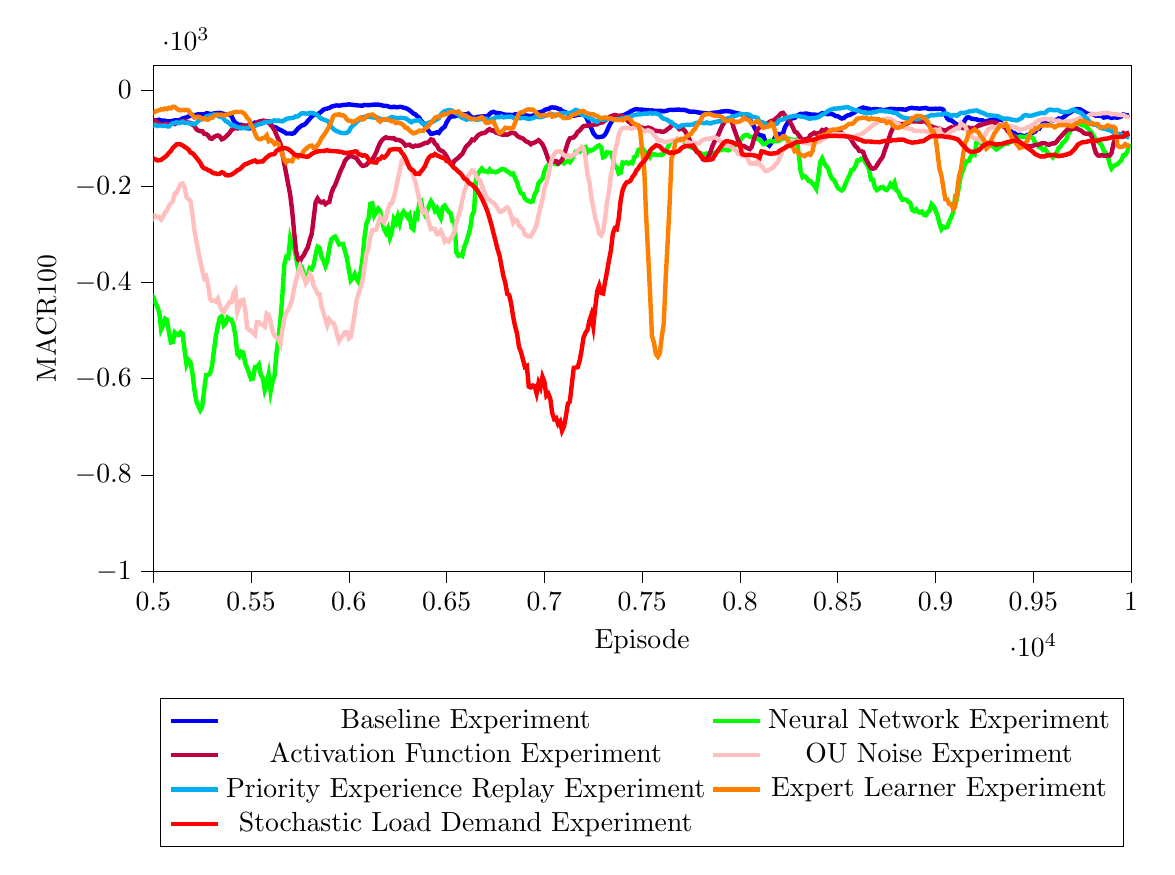
\begin{tikzpicture}

\definecolor{color0}{rgb}{1,0.498039215686275,0.0549019607843137}
\definecolor{color1}{rgb}{0.12156862745098,0.466666666666667,0.705882352941177}

\begin{axis}[
compat=newest,
tick align=outside,
tick pos=left,
x grid style={white!69.0196078431373!black},
xmin=5000, xmax=10000,
xtick style={color=black},
y grid style={white!69.0196078431373!black},
ymin=-1000.00, ymax=50.00,
ytick style={color=black},
scaled y ticks=true,
scaled y ticks=base 10:-3,
width=14cm,
height=8cm,
xlabel=Episode,
ylabel=MACR100,
%y label style={at={(-0.2,0.5)}}
%legend pos=south east
legend columns=2,
legend style={at={(0.5,-0.25)},anchor=north}
]

\addplot [ultra thick, blue]
table {%
100 -1582.67067718997
110 -1683.01661596282
120 -1790.32405198101
130 -1719.45505368521
140 -1626.98913277438
150 -1565.74285100258
160 -1418.63315026896
170 -1371.80179916204
180 -1375.93924454321
190 -1345.46802417995
200 -1298.37396567856
210 -1193.14672097731
220 -1139.18974455561
230 -1168.83869968173
240 -1172.51147639978
250 -1168.13326544273
260 -1245.39875298235
270 -1303.16914844481
280 -1324.62036687109
290 -1354.06203288941
300 -1389.75254102123
310 -1393.8006463874
320 -1355.15305241583
330 -1311.11801617452
340 -1283.81636104541
350 -1219.64857747229
360 -1189.39125920986
370 -1113.86327240352
380 -1062.58838313853
390 -1031.85292795208
400 -958.144683185093
410 -903.117037009552
420 -871.626221316283
430 -831.302898389944
440 -763.841713296356
450 -724.794912013634
460 -659.416291918026
470 -609.688945607528
480 -549.865720029054
490 -476.247230741856
500 -437.928122162497
510 -421.569590654568
520 -411.202150282573
530 -388.304445701138
540 -374.749589238142
550 -362.886271385558
560 -347.596375581264
570 -359.99439814117
580 -344.471662650798
590 -342.856988696357
600 -342.609112249219
610 -336.306884815506
620 -338.623330229533
630 -321.162498138758
640 -301.841472871826
650 -290.037860479904
660 -299.222975781901
670 -305.734249260761
680 -287.272937068945
690 -273.380943968795
700 -262.731331361897
710 -237.221636611637
720 -215.288745999989
730 -227.27084028216
740 -235.426467129444
750 -258.290633844516
760 -289.037785015782
770 -256.019760645466
780 -254.985715886778
790 -254.544580722355
800 -262.352660976914
810 -268.927054447971
820 -267.3622969706
830 -270.41158495355
840 -278.076802614562
850 -270.538887467588
860 -227.752489432417
870 -244.934563245234
880 -267.372165644971
890 -280.525712729855
900 -278.457870859474
910 -274.41286096963
920 -305.858625936095
930 -319.593726469206
940 -342.036494103142
950 -370.369579555932
960 -367.93461225045
970 -386.126320813181
980 -414.995185456001
990 -430.932935656827
1000 -466.023097142712
1010 -495.411388378483
1020 -495.274861982452
1030 -494.843471850286
1040 -503.195540774119
1050 -469.326791324352
1060 -456.772718548918
1070 -420.818247819788
1080 -372.879438253286
1090 -348.419622014437
1100 -312.493536392746
1110 -278.476110680835
1120 -237.61422343003
1130 -211.017825111322
1140 -190.086697842075
1150 -199.545851485636
1160 -228.246796984409
1170 -263.955985758992
1180 -275.83735276978
1190 -285.850661920318
1200 -296.433006589283
1210 -315.601032720507
1220 -342.004246670694
1230 -379.34944387675
1240 -392.21070745744
1250 -398.114404399303
1260 -392.363697960248
1270 -383.14810111568
1280 -403.153410577432
1290 -421.350037845288
1300 -425.799280742711
1310 -435.631891803026
1320 -440.057409618591
1330 -438.755964980269
1340 -440.400017038213
1350 -463.90647170706
1360 -492.316321906948
1370 -512.143403348786
1380 -517.977975597813
1390 -529.752984645077
1400 -561.327278654748
1410 -571.885038583095
1420 -597.160630037091
1430 -592.879697765281
1440 -596.935632128831
1450 -576.798991420391
1460 -549.756336313763
1470 -520.969912474083
1480 -474.956556261303
1490 -425.020786876369
1500 -366.896548969839
1510 -339.830558284878
1520 -307.657739786659
1530 -326.513121833339
1540 -321.136532201672
1550 -343.088031840243
1560 -347.167494836874
1570 -371.659470497533
1580 -408.12488681439
1590 -419.280179664721
1600 -452.629562227878
1610 -445.243604889162
1620 -445.902768661632
1630 -418.280330540036
1640 -418.25449592165
1650 -402.12723072398
1660 -378.79468412438
1670 -338.334652392152
1680 -310.378524053678
1690 -315.086155200922
1700 -296.530370627066
1710 -320.683399092035
1720 -331.294887046292
1730 -321.495539650028
1740 -294.759561548334
1750 -286.469097597911
1760 -325.353398229501
1770 -341.752884537435
1780 -380.240338294556
1790 -373.292171237719
1800 -373.367162501253
1810 -345.009544845194
1820 -309.194618115969
1830 -332.292448062209
1840 -348.810493918648
1850 -330.219327091073
1860 -287.614649023455
1870 -277.787459980014
1880 -235.112733807108
1890 -229.118185489735
1900 -222.693743899885
1910 -224.117006952648
1920 -242.495961935494
1930 -214.427796871159
1940 -206.827110185257
1950 -199.675472642288
1960 -209.892030149747
1970 -217.231369334064
1980 -231.522886226629
1990 -241.167074420684
2000 -260.271633992173
2010 -281.321713015892
2020 -273.374115270509
2030 -263.591236335077
2040 -249.819820273001
2050 -319.380737438235
2060 -322.323269161544
2070 -302.810686925109
2080 -284.748625073881
2090 -295.578880284771
2100 -288.238378202639
2110 -265.161740762822
2120 -268.024110032228
2130 -302.429999440736
2140 -306.666255310436
2150 -269.233026763541
2160 -262.909217013058
2170 -273.623549685475
2180 -284.865581507639
2190 -275.056104293059
2200 -274.743205711238
2210 -283.468327617398
2220 -284.760679399697
2230 -262.289852649385
2240 -267.060482968113
2250 -252.055379128414
2260 -250.140331882108
2270 -270.351222107432
2280 -271.629500432955
2290 -290.346483924833
2300 -290.557632069583
2310 -284.703497982845
2320 -278.163493441099
2330 -275.22758920903
2340 -270.504331669207
2350 -256.06377864296
2360 -259.905656155084
2370 -234.326966851875
2380 -235.211222902817
2390 -212.956179153673
2400 -201.035392036018
2410 -201.879593406299
2420 -210.632141013534
2430 -212.682092755533
2440 -211.664034434221
2450 -212.039578410957
2460 -201.164251590499
2470 -223.69480939201
2480 -235.791813807977
2490 -235.801873631489
2500 -245.720288902059
2510 -271.670971640323
2520 -265.960441535536
2530 -267.752736332204
2540 -283.029587155131
2550 -295.216759915082
2560 -305.658949633758
2570 -309.812516022472
2580 -304.645053665964
2590 -308.724849169679
2600 -303.720264326949
2610 -283.893513482523
2620 -279.508321263278
2630 -275.252920069183
2640 -255.301870154833
2650 -252.13561140203
2660 -245.884157327538
2670 -222.701827882466
2680 -213.12881130163
2690 -214.563639073429
2700 -213.32222344502
2710 -208.726965560738
2720 -208.95027804936
2730 -224.260178783552
2740 -231.604888074256
2750 -228.719045191698
2760 -228.144453947858
2770 -228.467898749956
2780 -228.416030312146
2790 -218.785791486099
2800 -214.282647346688
2810 -210.237538071453
2820 -203.851467421057
2830 -186.221888290546
2840 -184.886209517516
2850 -183.531120132589
2860 -183.936797669516
2870 -182.298940620261
2880 -175.900033546734
2890 -174.372263643375
2900 -174.666425971798
2910 -171.929918493861
2920 -172.070841279777
2930 -170.186558377889
2940 -167.208864346754
2950 -168.428425934892
2960 -166.642953898677
2970 -163.525968696425
2980 -169.088785730215
2990 -186.402150878789
3000 -192.08186610154
3010 -197.732452194642
3020 -206.823595565347
3030 -215.152914875902
3040 -218.974528280641
3050 -221.604742185156
3060 -222.659062020588
3070 -223.429861204943
3080 -221.227375918372
3090 -206.184480088583
3100 -204.473498304225
3110 -205.58129285553
3120 -211.638744873524
3130 -209.592179178117
3140 -208.437553546729
3150 -201.273489357124
3160 -199.889365036957
3170 -194.928328330463
3180 -194.939608705649
3190 -192.181282574995
3200 -181.975716767485
3210 -177.046098059833
3220 -157.394944799463
3230 -142.55543540218
3240 -133.127945538735
3250 -125.795270162001
3260 -119.983627841475
3270 -116.769864098626
3280 -113.500020433746
3290 -114.632299043104
3300 -113.348353860625
3310 -114.450739042082
3320 -119.34336673635
3330 -119.743688954468
3340 -115.228182692882
3350 -122.596067546833
3360 -126.569043563297
3370 -131.816620736589
3380 -129.548112115645
3390 -127.31638180272
3400 -127.074630080849
3410 -119.909798241126
3420 -110.493639085367
3430 -113.882451740619
3440 -114.460529910085
3450 -112.965335469546
3460 -121.683466206909
3470 -120.420367262974
3480 -123.332787959531
3490 -123.785886203402
3500 -128.181802400406
3510 -135.154761577217
3520 -151.204842329858
3530 -157.406556941784
3540 -163.000279819976
3550 -164.376720179473
3560 -149.011784907347
3570 -146.703637492454
3580 -142.912463172943
3590 -141.004768030757
3600 -137.031833657044
3610 -125.604904549699
3620 -112.31830170616
3630 -106.934096482904
3640 -105.770307019033
3650 -98.3601507720995
3660 -94.6189018569445
3670 -93.2379216335991
3680 -97.4854500086007
3690 -94.7956026618083
3700 -101.054676556018
3710 -104.139055712494
3720 -105.173627127699
3730 -98.7324856474767
3740 -91.7910175051864
3750 -89.5067959069137
3760 -93.7906550370732
3770 -91.2585029493566
3780 -84.7386996188514
3790 -84.8920508704731
3800 -77.7481059799439
3810 -81.0518759029136
3820 -80.6375478422508
3830 -83.305054907553
3840 -86.957600431416
3850 -84.3344457558337
3860 -83.417847669054
3870 -82.0533710592254
3880 -82.2737108033426
3890 -81.3022894436904
3900 -80.6421167117979
3910 -75.3495754868415
3920 -74.6447742182263
3930 -71.1823259725353
3940 -71.4046110747159
3950 -72.2002359622907
3960 -71.4122885162793
3970 -73.8583326086436
3980 -74.7926558648821
3990 -74.8235873775421
4000 -79.6589519801103
4010 -80.6653416996501
4020 -81.9910865814821
4030 -88.6685363190144
4040 -87.9870393473489
4050 -91.7290038517164
4060 -92.0304508887788
4070 -87.1726294343971
4080 -84.0096099298739
4090 -82.4434542026448
4100 -76.9178300172877
4110 -75.9659340706354
4120 -73.0419323815056
4130 -66.1683058954311
4140 -61.5171329725077
4150 -58.0414227446071
4160 -59.6366342819378
4170 -65.3518725230383
4180 -64.2903120299829
4190 -62.170949627593
4200 -60.9690899765004
4210 -61.7475030294262
4220 -63.4418538588015
4230 -67.4182190383501
4240 -69.5015120537565
4250 -71.1171769650569
4260 -68.9745600819291
4270 -67.6923615495467
4280 -69.2062754705215
4290 -72.2229942488348
4300 -73.7309605352163
4310 -74.3421509608227
4320 -72.6723669126953
4330 -68.2763636547142
4340 -66.1794602816536
4350 -66.8508314211425
4360 -69.1909275320167
4370 -69.914244341478
4380 -72.3182028209903
4390 -73.9654523756489
4400 -76.5063544579275
4410 -76.0090014582169
4420 -76.9866313369579
4430 -77.7123452305967
4440 -79.8655175719816
4450 -79.8819061259388
4460 -81.3310272881013
4470 -82.9292284920693
4480 -83.5075050725013
4490 -83.1321830895641
4500 -83.3880028748841
4510 -86.1944721076755
4520 -87.7626946441184
4530 -91.9142412285789
4540 -95.2047396170913
4550 -98.0319201471644
4560 -97.292684787028
4570 -99.5200546918774
4580 -101.648666182904
4590 -104.864248962576
4600 -105.315707910302
4610 -107.444656438088
4620 -110.115810041797
4630 -109.558114872071
4640 -107.650085422161
4650 -107.949582267444
4660 -108.365029520186
4670 -104.94164922091
4680 -103.028565105648
4690 -100.408461081914
4700 -99.0910381098535
4710 -96.773492220205
4720 -94.4795040621003
4730 -92.1256180175491
4740 -92.9307752766569
4750 -89.24366544151
4760 -85.7622040409979
4770 -84.4018926764698
4780 -79.8254541045513
4790 -77.2767105106706
4800 -73.5093328325265
4810 -69.9824992584099
4820 -67.7108002679934
4830 -67.6788554566407
4840 -65.259831714292
4850 -65.6375638400439
4860 -67.1596614319916
4870 -70.0786076389502
4880 -73.4670382059555
4890 -74.8039514467491
4900 -76.720579367597
4910 -79.1307388211305
4920 -80.2129389792409
4930 -79.3834268470602
4940 -77.4487682863027
4950 -76.8949653435574
4960 -75.0433910270948
4970 -70.8376394298899
4980 -69.0709116706586
4990 -67.2867537762524
5000 -66.0062445785087
5010 -64.2356095142854
5020 -62.4178997164067
5030 -61.858784989549
5040 -63.7651970627801
5050 -63.5995306568269
5060 -63.8827468492901
5070 -65.2337550582829
5080 -65.3424844326781
5090 -64.79173798177
5100 -64.2161158452
5110 -62.8910374289195
5120 -62.9054502453101
5130 -62.9913308297181
5140 -61.6654152846916
5150 -59.2238388742374
5160 -57.8884803312027
5170 -56.9673224338068
5180 -54.9826860509792
5190 -53.3256464355382
5200 -52.6495575624033
5210 -52.2820442907199
5220 -51.6036676358072
5230 -50.4668263983367
5240 -50.3455743227576
5250 -50.8507617603289
5260 -50.9091971993702
5270 -48.7505957710019
5280 -48.8015350760557
5290 -49.8554590215925
5300 -49.9947980538754
5310 -48.7970913001391
5320 -48.3174511762648
5330 -48.1612806372053
5340 -47.4848483104001
5350 -48.5940828418557
5360 -49.4982071636755
5370 -50.8102270049599
5380 -50.8886989060334
5390 -51.8954960460939
5400 -53.8705960665776
5410 -63.3784639985168
5420 -68.0248120298137
5430 -70.604612702302
5440 -72.8789157785191
5450 -72.3359162518416
5460 -74.6183082009752
5470 -77.8902173111466
5480 -79.4723182838563
5490 -79.7303163799689
5500 -79.3860250935761
5510 -70.8675360277044
5520 -67.8366091808934
5530 -68.8128370212522
5540 -68.4901802165153
5550 -70.228451601817
5560 -68.4769207602082
5570 -66.7186217968063
5580 -65.6619108660218
5590 -68.2432338765906
5600 -70.9754782762023
5610 -75.759806710296
5620 -77.2630334627835
5630 -78.2048654970101
5640 -81.5098764836914
5650 -82.7922319713212
5660 -85.3751834428602
5670 -87.2220167345552
5680 -90.4701685791981
5690 -90.5176232985753
5700 -90.4016448053658
5710 -90.8728144015257
5720 -89.505723829302
5730 -85.0741775731696
5740 -80.0350759610018
5750 -76.7745418991211
5760 -73.6827818327752
5770 -72.5775766416263
5780 -69.4274947449414
5790 -64.4178694560071
5800 -59.8931888190726
5810 -55.1518252225498
5820 -51.9840531031113
5830 -51.1700304657991
5840 -50.0516801513371
5850 -47.8931286351632
5860 -44.7285981442628
5870 -40.9912152729706
5880 -39.3830329265479
5890 -38.6056544278679
5900 -37.4158518977135
5910 -34.7670070195527
5920 -33.7900968025427
5930 -32.538797480679
5940 -32.1443895358714
5950 -32.4413949550762
5960 -32.1106551875129
5970 -31.1659989713503
5980 -30.9222744797693
5990 -30.6442108778978
6000 -29.8577574624616
6010 -30.4588917814229
6020 -30.9195401202094
6030 -31.4638529532879
6040 -31.6901337207816
6050 -32.2952773493988
6060 -32.3998812804375
6070 -32.5478531369155
6080 -31.1595483730785
6090 -31.362658106716
6100 -31.6705375660556
6110 -31.303237397704
6120 -30.6506880259579
6130 -30.5852532228118
6140 -30.2831232769191
6150 -30.3454150109023
6160 -31.2088494103889
6170 -32.1049361613171
6180 -33.0672372692728
6190 -32.8852740533577
6200 -33.9749215072918
6210 -35.3874943782744
6220 -35.8027882332673
6230 -34.8350142467746
6240 -35.7831185102669
6250 -35.8840480717573
6260 -35.0932439782184
6270 -35.5168257271323
6280 -36.7145080604008
6290 -37.7325464680847
6300 -39.2961006544063
6310 -42.0908647264308
6320 -45.2175661515425
6330 -49.0064276290005
6340 -50.736726101735
6350 -54.6884641491145
6360 -57.5974664174039
6370 -64.3678910042704
6380 -68.6887176648432
6390 -73.3404301296328
6400 -81.0629889957926
6410 -86.334074606319
6420 -91.2048140666506
6430 -90.4805068494712
6440 -89.3082571154534
6450 -87.9914425979375
6460 -89.3267401721438
6470 -83.1355409987879
6480 -79.4783468266079
6490 -76.3967181682066
6500 -67.3146380653495
6510 -60.7473252288909
6520 -54.832944557267
6530 -54.6966527099979
6540 -54.8718273397648
6550 -53.4411978157749
6560 -52.5227188683764
6570 -52.0545052860058
6580 -51.8518547535337
6590 -50.8061658429373
6600 -50.7128764061664
6610 -49.1986320537212
6620 -53.8851734606177
6630 -56.8960128683541
6640 -58.2432949327712
6650 -57.0192010294538
6660 -55.8642272220796
6670 -55.5424066918378
6680 -54.6785069194974
6690 -54.5793924788436
6700 -54.7555536902297
6710 -54.7590205896654
6720 -49.784134294059
6730 -46.5938859743494
6740 -45.4210622925335
6750 -47.377681421288
6760 -47.8377971605892
6770 -48.3198498402635
6780 -49.1139059043615
6790 -50.6432451918163
6800 -51.1745565663832
6810 -51.9406087117671
6820 -51.5379433886983
6830 -52.0628258632027
6840 -52.0348363757668
6850 -50.6109181461511
6860 -51.0212503041207
6870 -52.4984753792981
6880 -53.0291003761799
6890 -51.7876488975975
6900 -52.5413890120119
6910 -53.2336773046502
6920 -53.6238405730956
6930 -54.4767950271511
6940 -53.3456441545895
6950 -52.2670357576675
6960 -50.3796872119862
6970 -46.7096484806409
6980 -45.6395068164474
6990 -44.990415542909
7000 -41.9699684365999
7010 -40.0657104038903
7020 -39.6419967459206
7030 -36.8940356740202
7040 -36.183043805733
7050 -36.7342108686288
7060 -36.8928435667169
7070 -39.1025271366987
7080 -39.6042127679189
7090 -43.7530306875594
7100 -45.2755496361732
7110 -46.7029365938239
7120 -48.5253787800753
7130 -52.5431088398961
7140 -53.5482365852415
7150 -53.4424240378167
7160 -52.7381529997394
7170 -51.0824645953071
7180 -51.167176677208
7190 -49.1641414377892
7200 -51.2684737987661
7210 -54.1387016383617
7220 -62.1449246218163
7230 -70.6300193915608
7240 -80.0965497935702
7250 -89.4400333183476
7260 -94.8723169896571
7270 -98.0834282545216
7280 -98.1648300728078
7290 -97.2800209165531
7300 -96.5141151440269
7310 -92.6553759414554
7320 -85.0897622833283
7330 -75.3970910220413
7340 -68.0906856043869
7350 -61.511061235205
7360 -58.3135319725659
7370 -56.8461924320276
7380 -55.7451798134924
7390 -54.5683199786443
7400 -52.6825045348189
7410 -51.5515932079195
7420 -49.3740885788288
7430 -47.3847007937568
7440 -44.5978563986054
7450 -42.7172546360163
7460 -40.6670880619704
7470 -39.9937243406633
7480 -40.4996369014487
7490 -40.5728328260648
7500 -40.9083829178696
7510 -41.5314000143918
7520 -41.9811802452164
7530 -41.7317887268957
7540 -42.9781138764213
7550 -42.402698763123
7560 -43.0342591089058
7570 -43.4528485921213
7580 -43.5483599928163
7590 -43.2339827003805
7600 -43.5020657072571
7610 -44.5387995843794
7620 -43.4578196079557
7630 -42.6756459899397
7640 -41.1519646918036
7650 -41.1663435573435
7660 -41.3348891721394
7670 -41.1091830485161
7680 -40.6653833942659
7690 -40.9185427399245
7700 -41.4520708345876
7710 -41.1485416196148
7720 -41.9355795773992
7730 -43.2061834830825
7740 -44.770006056072
7750 -45.2781123351702
7760 -45.0448202156887
7770 -45.3964201162332
7780 -46.0833402633052
7790 -46.9839925532765
7800 -47.2908910542404
7810 -47.8662939228585
7820 -48.273559238949
7830 -48.6671263793997
7840 -48.3942347117362
7850 -48.2618077970395
7860 -47.6191468444484
7870 -47.0623301309628
7880 -46.778161291281
7890 -46.4189043495608
7900 -45.153791735951
7910 -44.7276886766073
7920 -44.4046854086779
7930 -43.7333507179061
7940 -44.2640781414381
7950 -44.6395587906615
7960 -45.6717804482887
7970 -46.9097925066285
7980 -47.8001763267066
7990 -48.8020713522956
8000 -49.6471266542728
8010 -50.7222272750426
8020 -52.6049576230956
8030 -54.5534758127876
8040 -56.3941666695212
8050 -59.7196519730978
8060 -69.433721381769
8070 -74.705393747914
8080 -83.1552712736591
8090 -90.9342571908836
8100 -93.1521711343762
8110 -94.7507178578763
8120 -95.4471921188058
8130 -107.490780696229
8140 -112.57448987948
8150 -115.719323836258
8160 -110.206741154575
8170 -105.831255232785
8180 -97.9503206154232
8190 -91.2848577797891
8200 -91.8792943852934
8210 -91.4217747350236
8220 -90.1019094750537
8230 -77.4337244706063
8240 -70.5255752433229
8250 -63.884156157077
8260 -60.1792771790744
8270 -58.6274915902902
8280 -57.8048191073041
8290 -54.1817414551567
8300 -51.6852914652937
8310 -49.6341363039117
8320 -50.1592299029182
8330 -49.2750727289415
8340 -48.9668844931043
8350 -50.0930933011138
8360 -50.8547861795101
8370 -50.9920878184924
8380 -50.9429668035475
8390 -51.8954805177735
8400 -51.8966774335891
8410 -51.069798160704
8420 -48.1249231144832
8430 -48.4613823220187
8440 -49.7704781509272
8450 -50.3047767488847
8460 -49.4549233780753
8470 -50.205256112584
8480 -51.63940159385
8490 -54.4734411124089
8500 -54.7566842478969
8510 -57.1891134195153
8520 -59.264206273908
8530 -58.4979334549901
8540 -55.2530684213869
8550 -52.8572743251877
8560 -52.2038840210126
8570 -49.6378185185264
8580 -48.1884103902173
8590 -45.3540690762375
8600 -42.5158569473808
8610 -39.6556221717415
8620 -37.9011862869643
8630 -36.4057821962929
8640 -37.8129641032016
8650 -38.5322013483772
8660 -39.2483445335646
8670 -41.3655207690731
8680 -40.1616886302575
8690 -39.5377570213198
8700 -40.0318252106524
8710 -40.5238492330108
8720 -40.7849118764841
8730 -41.9793319451388
8740 -41.6245177756549
8750 -40.9270169670041
8760 -40.3423004633666
8770 -39.0975649634203
8780 -39.7812075629185
8790 -39.4915568333693
8800 -40.7701076097111
8810 -39.9516840272335
8820 -40.1260439902027
8830 -40.151139058642
8840 -40.801492393622
8850 -40.8197981282041
8860 -38.856968836868
8870 -37.5708752970098
8880 -37.1176510346396
8890 -37.9865453605945
8900 -38.0408276882926
8910 -38.4420940133236
8920 -38.7174370046658
8930 -38.0597472028034
8940 -37.8113390049934
8950 -37.3019830503828
8960 -38.8327827249377
8970 -39.6114732959965
8980 -39.283089698803
8990 -39.4643053946413
9000 -38.876616249837
9010 -39.2807599212262
9020 -38.7900174353582
9030 -39.1673868928163
9040 -40.9678754502991
9050 -52.0812571635984
9060 -59.1745160971745
9070 -62.5318171979986
9080 -62.982616863777
9090 -66.0627949514704
9100 -69.2355804296836
9110 -71.9444601030274
9120 -73.4333767724736
9130 -74.1208157485611
9140 -72.6596061014741
9150 -62.4764624649673
9160 -57.5187065377309
9170 -56.7850193805757
9180 -59.1258246393433
9190 -60.0478095561797
9200 -60.5436788188946
9210 -61.0137390509708
9220 -62.5862303514518
9230 -63.0210684865312
9240 -63.1837755295856
9250 -66.0292137657093
9260 -64.9899800911894
9270 -63.5964463414252
9280 -63.1155602918193
9290 -61.5576470629439
9300 -61.1905124076157
9310 -60.3280963986082
9320 -60.663754903807
9330 -65.0919933602395
9340 -69.8683746960272
9350 -71.666575014798
9360 -77.562698243032
9370 -81.2037132104092
9380 -83.5074923485987
9390 -88.1104241576331
9400 -89.0149029646352
9410 -91.3777453392196
9420 -95.2666487348928
9430 -93.1993951550064
9440 -94.5106646468401
9450 -95.339530456306
9460 -96.0066717170614
9470 -93.2337781715456
9480 -93.4375486809685
9490 -90.3410621543092
9500 -88.0909818769091
9510 -86.0650128871423
9520 -81.0945073930937
9530 -80.5887543614218
9540 -73.9839863388628
9550 -69.4488556304241
9560 -63.9079188973925
9570 -65.0074662633097
9580 -63.3236143902492
9590 -61.3253124369118
9600 -63.1986748008318
9610 -62.56274784161
9620 -61.7950950004923
9630 -59.2055552288645
9640 -59.4208756060733
9650 -57.7002166939177
9660 -54.86089736871
9670 -51.6523349821742
9680 -48.6989003560323
9690 -46.6769223364062
9700 -43.4846833067315
9710 -41.5465317731458
9720 -39.5833251761183
9730 -39.8041104786821
9740 -40.3585207802328
9750 -42.9875689864927
9760 -45.3118090880241
9770 -48.1315106911242
9780 -49.6650139675976
9790 -49.9630655243978
9800 -50.0768958365047
9810 -51.6359670468791
9820 -53.6575482843235
9830 -53.4081454482822
9840 -54.0645125929795
9850 -54.1212254606915
9860 -57.3507027410792
9870 -56.5566417999114
9880 -55.6976556148412
9890 -56.6622397534912
9900 -58.0386359343147
9910 -57.0727955944308
9920 -57.1649801613559
9930 -57.4337111290273
9940 -56.5958698424054
9950 -54.9802346597329
9960 -50.6783057083071
9970 -51.9937599131461
9980 -53.0358714672779
9990 -51.9429675482224
};
\addlegendentry{Baseline Experiment};

\addplot [ultra thick, green]
table {%
100 -661.211198352562
110 -510.414824746467
120 -470.76979275499
130 -497.012993380684
140 -492.878681964999
150 -518.934872561699
160 -511.906108276126
170 -532.832252895219
180 -571.765786087371
190 -590.117106682631
200 -649.837829844334
210 -624.333990353201
220 -625.591427558135
230 -628.557781903831
240 -596.917380227496
250 -572.156602168379
260 -561.596947917115
270 -532.389763776996
280 -496.792866211156
290 -507.249291682043
300 -491.799028167067
310 -497.945778281478
320 -593.301217939018
330 -639.65663113258
340 -696.868644735164
350 -715.234247545971
360 -756.616266353991
370 -778.998181421048
380 -798.109999424621
390 -811.974906818811
400 -828.633552573387
410 -839.691713959648
420 -727.555142634258
430 -649.427922821371
440 -561.01054439061
450 -517.81461254109
460 -470.085828269258
470 -441.348969301321
480 -401.299733797528
490 -351.201831151891
500 -286.1957905704
510 -228.988414852989
520 -235.387403757218
530 -237.649067316896
540 -250.918260936196
550 -258.723855252519
560 -269.336301721212
570 -282.50843174941
580 -293.329897354797
590 -294.472782205734
600 -288.216513982923
610 -291.820346491314
620 -292.934558773569
630 -305.391963789609
640 -294.525750137551
650 -303.550120332376
660 -305.965076660499
670 -304.780746499793
680 -322.923238275935
690 -334.487485853468
700 -336.310679660893
710 -334.910279123165
720 -320.333116805095
730 -321.481937571448
740 -408.288090494983
750 -440.132163638028
760 -497.211842046676
770 -547.573248843904
780 -584.685828953374
790 -639.768175854434
800 -691.554865317769
810 -750.52558432406
820 -812.78914355301
830 -893.566539212693
840 -919.652792451127
850 -966.909379066824
860 -968.930646403668
870 -1010.92734599578
880 -1050.03334574949
890 -1072.06776722333
900 -1114.12277899768
910 -1146.39832853046
920 -1174.82681789717
930 -1156.12949745221
940 -1123.81425231731
950 -1124.1922044245
960 -1168.80479093305
970 -1174.93644051927
980 -1190.29975641955
990 -1231.6308387323
1000 -1323.98147460055
1010 -1334.28112387202
1020 -1355.73045393042
1030 -1488.31732135475
1040 -1692.62906066324
1050 -1901.76299866931
1060 -2010.98441239885
1070 -1942.18275338525
1080 -1956.20647528332
1090 -1981.88246795577
1100 -1956.09821480125
1110 -1976.56090166537
1120 -1981.49134144711
1130 -1879.53673282067
1140 -1655.07987565588
1150 -1348.53547683256
1160 -1155.09183651449
1170 -1109.23797968827
1180 -971.102412325105
1190 -803.713692848601
1200 -633.9073653273
1210 -501.78575800489
1220 -379.245941544275
1230 -252.236625053046
1240 -180.107469429334
1250 -174.709815941178
1260 -135.989908198215
1270 -131.028275499084
1280 -129.381056249873
1290 -128.118917495506
1300 -134.660303062392
1310 -148.683294014461
1320 -164.804999039831
1330 -182.041265350488
1340 -199.599657947935
1350 -216.364570341888
1360 -232.750729238765
1370 -252.118271533481
1380 -269.02947247977
1390 -284.385007385416
1400 -291.156782182756
1410 -292.605554123917
1420 -288.931478823457
1430 -287.582375180826
1440 -285.286221628134
1450 -282.102469268487
1460 -279.736123353194
1470 -274.614458326599
1480 -273.64113769148
1490 -274.050665706034
1500 -274.661947235603
1510 -276.050297514486
1520 -283.102886226479
1530 -285.48506143898
1540 -287.806774628926
1550 -287.812860351329
1560 -294.094076408172
1570 -297.945085594925
1580 -301.266436075001
1590 -306.67224697523
1600 -312.371292618646
1610 -314.171288891745
1620 -311.151492103813
1630 -317.877367626407
1640 -322.777002425389
1650 -325.053245513038
1660 -322.530038926722
1670 -328.282980931987
1680 -330.722144941128
1690 -329.349292229624
1700 -328.550551700145
1710 -330.039886207665
1720 -334.878102669541
1730 -335.394702722601
1740 -339.668578601828
1750 -348.305667518734
1760 -354.397886027931
1770 -355.988584128095
1780 -348.9182990428
1790 -339.697390726072
1800 -318.186582325473
1810 -304.358381071802
1820 -285.547857018684
1830 -260.610041824826
1840 -234.580432640294
1850 -211.297933744409
1860 -191.225505392764
1870 -190.293830117609
1880 -248.976225444947
1890 -308.6521723891
1900 -352.003525781195
1910 -399.145505625918
1920 -433.115067235882
1930 -470.793753448198
1940 -503.700743409949
1950 -548.379393195661
1960 -595.903821491409
1970 -630.667531042402
1980 -609.880467234302
1990 -617.295173236054
2000 -681.812497261494
2010 -745.883801868248
2020 -800.88273766285
2030 -889.797217750416
2040 -976.919808298055
2050 -1028.48235952539
2060 -1072.84252148007
2070 -1097.60642000095
2080 -1119.09830008635
2090 -1091.65904843711
2100 -1015.42063269514
2110 -947.66442014396
2120 -913.814973131786
2130 -830.301312233054
2140 -745.552836569109
2150 -678.425269338349
2160 -618.065886927634
2170 -567.329465482747
2180 -521.090698959239
2190 -515.189532009841
2200 -541.472555275144
2210 -593.085509420404
2220 -593.806804303526
2230 -583.214308793968
2240 -601.794056849873
2250 -604.846365864819
2260 -599.856925329718
2270 -593.828382771227
2280 -587.679247990226
2290 -568.789147131255
2300 -545.032319760234
2310 -469.742669109511
2320 -441.808924009043
2330 -447.638951192381
2340 -445.801772747589
2350 -446.93110566333
2360 -437.959751189854
2370 -426.212235338833
2380 -423.359881088906
2390 -415.342555092916
2400 -398.769833644391
2410 -387.973091544936
2420 -378.179002271507
2430 -352.363666734526
2440 -307.638471856446
2450 -283.193721965563
2460 -273.88199944999
2470 -273.772444840893
2480 -268.137240638328
2490 -262.966089088705
2500 -257.394873312476
2510 -252.291223895367
2520 -240.435320891596
2530 -238.541522219095
2540 -239.923843906862
2550 -237.867757321121
2560 -232.975079010689
2570 -218.557443165806
2580 -204.744021238005
2590 -192.924960823874
2600 -185.474372219393
2610 -182.924964193769
2620 -172.277602025578
2630 -161.931759836203
2640 -153.732856932511
2650 -143.513982284697
2660 -136.743943421967
2670 -172.769722060312
2680 -206.07463653087
2690 -277.693978054895
2700 -388.197467440093
2710 -501.535138556189
2720 -566.186237773298
2730 -610.450737542565
2740 -656.046397250329
2750 -703.39386366739
2760 -772.293626376771
2770 -790.52882788317
2780 -814.472026228515
2790 -795.673813665407
2800 -741.189541781122
2810 -691.527373857725
2820 -665.006274488545
2830 -663.209885558729
2840 -666.617501296868
2850 -633.176157550006
2860 -592.623995078505
2870 -544.410971962755
2880 -491.814390123982
2890 -442.370900136586
2900 -388.359039453403
2910 -325.833349733432
2920 -350.137353763263
2930 -362.175317469959
2940 -359.69815788569
2950 -401.418242479335
2960 -445.905291951636
2970 -458.358553461385
2980 -463.746812283645
2990 -481.590779366926
3000 -547.24813174146
3010 -635.519179405474
3020 -676.856486129539
3030 -689.625014350321
3040 -734.70894416608
3050 -719.543265789518
3060 -654.729428613999
3070 -692.367496038295
3080 -689.924524065558
3090 -673.534605519004
3100 -609.105287355786
3110 -538.793049602811
3120 -519.860529692619
3130 -540.334358491327
3140 -515.994776036119
3150 -487.656677830105
3160 -488.748398096884
3170 -506.695654315099
3180 -569.918632292649
3190 -571.452925932871
3200 -583.886225280431
3210 -590.578459319718
3220 -516.409281183034
3230 -473.843876620921
3240 -438.110761102049
3250 -433.68884867668
3260 -440.424823727214
3270 -375.031358378059
3280 -314.54604489639
3290 -317.789132232807
3300 -300.37641784937
3310 -273.516312054933
3320 -272.357670292017
3330 -229.943208957252
3340 -197.126319035596
3350 -194.208377712102
3360 -183.010876254977
3370 -182.23651858507
3380 -178.333276177618
3390 -171.004441550482
3400 -178.978670227556
3410 -184.883846741934
3420 -180.190814096924
3430 -188.375222162127
3440 -205.839889304759
3450 -220.196722266731
3460 -236.834720041724
3470 -249.626854002563
3480 -258.084549398804
3490 -281.733575909892
3500 -292.68281860287
3510 -298.29266244149
3520 -313.255206976525
3530 -319.873721576998
3540 -325.552703854193
3550 -327.472491900025
3560 -325.41405881713
3570 -322.732887999516
3580 -327.309651754146
3590 -304.280627862771
3600 -294.317357988605
3610 -290.574284759957
3620 -287.204905726799
3630 -281.458988813212
3640 -261.567379683735
3650 -246.534623440111
3660 -227.034568943989
3670 -210.517348190235
3680 -198.428862466992
3690 -193.973684114211
3700 -184.973871081164
3710 -175.625461871311
3720 -165.231988499273
3730 -160.539389931934
3740 -163.904049095845
3750 -168.592551395749
3760 -186.17040724389
3770 -202.606721888143
3780 -218.441378691645
3790 -237.985649242744
3800 -260.240041584239
3810 -279.344016775391
3820 -302.663264724154
3830 -323.358685450128
3840 -345.532113480092
3850 -362.208518665432
3860 -387.199444073776
3870 -404.580664541386
3880 -420.407338956729
3890 -433.545724601355
3900 -434.065663627895
3910 -449.034606850055
3920 -458.702517328848
3930 -462.049351271984
3940 -471.895487282625
3950 -491.575759464177
3960 -499.369849654742
3970 -505.235626008243
3980 -517.115622591548
3990 -509.639571874635
4000 -518.858510501282
4010 -528.306822470593
4020 -551.883903524262
4030 -583.396664749721
4040 -575.723514215948
4050 -592.732904202639
4060 -597.716610025016
4070 -589.576774030534
4080 -579.431167687291
4090 -600.150467739329
4100 -610.390245150874
4110 -597.617332766734
4120 -583.525759380858
4130 -602.423296527611
4140 -648.694453525404
4150 -651.405235700465
4160 -631.580233805752
4170 -624.4793607081
4180 -634.997825410705
4190 -600.262250688081
4200 -574.412462703566
4210 -561.31604361614
4220 -534.877417203748
4230 -497.706422768372
4240 -464.885740788371
4250 -444.17639383454
4260 -434.270344580735
4270 -436.378262712633
4280 -402.931644434339
4290 -428.818447921522
4300 -432.422955033524
4310 -427.235153353478
4320 -433.587037655223
4330 -431.261682919507
4340 -427.104955791664
4350 -398.776651898715
4360 -400.413003157674
4370 -401.344593374561
4380 -427.233424392161
4390 -412.082814887888
4400 -413.825738035173
4410 -443.85691429287
4420 -478.404677246412
4430 -454.991106080138
4440 -432.669679450124
4450 -439.201976540884
4460 -440.889500317766
4470 -427.415893327343
4480 -394.089900588133
4490 -381.388921836169
4500 -367.081693010622
4510 -329.079040388699
4520 -276.182092996015
4530 -272.52148461873
4540 -267.448441271108
4550 -258.829978384671
4560 -249.923139109684
4570 -250.133393132478
4580 -260.739432142197
4590 -271.014544350669
4600 -281.479390146454
4610 -304.626697417363
4620 -324.479841898669
4630 -342.970260001762
4640 -388.78639547876
4650 -438.772467745616
4660 -506.559053542806
4670 -579.166139821015
4680 -657.306426690796
4690 -717.080250594399
4700 -752.169970255066
4710 -777.391883567583
4720 -815.001373769649
4730 -805.359096601139
4740 -809.276867757064
4750 -793.963777273139
4760 -759.752356760064
4770 -701.409121077209
4780 -616.414173155211
4790 -562.410684801227
4800 -520.129137620647
4810 -485.078800406828
4820 -427.66799282566
4830 -439.824992339687
4840 -406.944884860208
4850 -384.083998596638
4860 -352.759595284997
4870 -358.451172916678
4880 -379.619165148942
4890 -369.865084457767
4900 -382.276270980597
4910 -392.318464950787
4920 -414.669264893708
4930 -401.07173613496
4940 -388.503596518738
4950 -422.818449373287
4960 -443.253578219595
4970 -437.250568945347
4980 -426.11222964904
4990 -424.224394080439
5000 -430.411248695825
5010 -441.322442194788
5020 -449.755069047754
5030 -461.216704457488
5040 -497.563039732449
5050 -488.440920855459
5060 -475.19724343786
5070 -477.734782414587
5080 -503.431142128545
5090 -524.648614876952
5100 -523.7715300463
5110 -503.820856554968
5120 -507.896314542374
5130 -509.208545052919
5140 -503.370985878872
5150 -506.551771025059
5160 -540.476602985007
5170 -570.388749838744
5180 -560.926496262527
5190 -565.784842185877
5200 -588.018004395631
5210 -622.497060012675
5220 -646.438280156285
5230 -656.579789816638
5240 -665.142455172933
5250 -657.7377503663
5260 -624.383974810728
5270 -592.353747169846
5280 -592.029165215115
5290 -589.202438816816
5300 -574.010978577068
5310 -541.762294802208
5320 -511.421260964103
5330 -490.01312563372
5340 -473.176728929902
5350 -470.155341670613
5360 -488.981699098716
5370 -485.045477712189
5380 -473.249338318457
5390 -476.255507184755
5400 -477.047325926359
5410 -488.155551682773
5420 -510.981176058094
5430 -548.194936183403
5440 -553.395971328168
5450 -543.928218175476
5460 -545.82999439052
5470 -568.021508219786
5480 -577.717950662838
5490 -588.353154318353
5500 -600.69105921968
5510 -599.565264706634
5520 -576.001231013662
5530 -576.099991354079
5540 -570.665441460562
5550 -591.83186648288
5560 -598.863963793581
5570 -623.702287872064
5580 -611.973181821145
5590 -591.343494878076
5600 -626.390818988931
5610 -605.516477678325
5620 -593.548974068957
5630 -547.295128567293
5640 -515.280563240333
5650 -477.480383599879
5660 -427.796269630954
5670 -362.54393393206
5680 -346.9983182378
5690 -348.672716254799
5700 -308.496239130043
5710 -323.601386660808
5720 -327.298740994251
5730 -347.994720411077
5740 -370.168897107874
5750 -363.720898775336
5760 -368.091209433957
5770 -386.086208268842
5780 -392.230282758518
5790 -385.654771154551
5800 -370.168667823553
5810 -372.072782835743
5820 -363.842076362246
5830 -342.388677405209
5840 -325.571094943686
5850 -327.868434084738
5860 -346.650022006175
5870 -354.300529526786
5880 -365.934041236909
5890 -355.250581851086
5900 -328.674124177341
5910 -310.797572150878
5920 -306.572518216108
5930 -304.516922133236
5940 -312.230714466183
5950 -321.143680191062
5960 -319.793608272032
5970 -320.007666163226
5980 -334.555050708756
5990 -349.6800207644
6000 -373.53287214033
6010 -395.71595471786
6020 -390.782666657965
6030 -382.291424932963
6040 -392.975383980178
6050 -399.538475193002
6060 -378.065674828048
6070 -350.133083998735
6080 -305.968478785389
6090 -277.168229971901
6100 -268.307466113272
6110 -236.38673288078
6120 -235.561702599499
6130 -260.884670962061
6140 -253.844445196241
6150 -246.738939345802
6160 -251.366854365682
6170 -274.134031032126
6180 -288.795433205106
6190 -297.0778865719
6200 -287.909455405788
6210 -307.196048140153
6220 -295.874891732517
6230 -268.39061542008
6240 -275.50200204305
6250 -262.379518811908
6260 -276.783481170067
6270 -259.067590117612
6280 -252.469047852378
6290 -258.187097313056
6300 -264.338332360962
6310 -259.158838349107
6320 -286.294766246528
6330 -289.585979887996
6340 -259.358944093789
6350 -263.860741263714
6360 -234.605475808036
6370 -231.463706288328
6380 -253.009841506135
6390 -260.001826266534
6400 -251.112580278295
6410 -240.243905704713
6420 -231.390374376377
6430 -238.209975086168
6440 -250.748577302173
6450 -245.734526257344
6460 -258.334578704654
6470 -266.14743054049
6480 -243.616150728324
6490 -240.142029051844
6500 -246.480557030288
6510 -253.008980312716
6520 -256.140906538523
6530 -272.744149789006
6540 -274.695122826451
6550 -337.879431005492
6560 -344.517556436642
6570 -342.423606840082
6580 -344.693494995186
6590 -326.35397427329
6600 -315.828193128794
6610 -303.175281920136
6620 -288.574719325454
6630 -260.475828087872
6640 -252.123146014107
6650 -185.668492745718
6660 -174.168578433268
6670 -168.211629289015
6680 -163.225585244797
6690 -168.455402444612
6700 -169.431401150698
6710 -170.520571463231
6720 -165.1371756787
6730 -169.775092935271
6740 -169.696652989331
6750 -171.139660815151
6760 -169.721464033696
6770 -167.327286475603
6780 -164.454925818401
6790 -164.309290377909
6800 -166.190915502289
6810 -169.412011987411
6820 -171.45095631225
6830 -175.139700637156
6840 -173.679859043327
6850 -182.826518288178
6860 -191.791397144467
6870 -205.308855297598
6880 -214.6673960806
6890 -215.871629087028
6900 -225.323986294019
6910 -229.479432462676
6920 -230.972531244721
6930 -232.661212332286
6940 -231.544755146165
6950 -216.735635797168
6960 -209.813397971778
6970 -193.485109148506
6980 -188.753590667421
6990 -184.501978088925
7000 -168.745392976024
7010 -159.904182296709
7020 -156.041399307689
7030 -145.596879638093
7040 -145.439937532977
7050 -153.039634623807
7060 -154.32772907142
7070 -154.141758396209
7080 -149.604351603225
7090 -148.68968007786
7100 -152.368220415407
7110 -149.710390873761
7120 -147.485043697748
7130 -149.985919202784
7140 -144.365904249065
7150 -135.693488827797
7160 -128.101383884314
7170 -127.529279167731
7180 -128.311292670869
7190 -123.990163997645
7200 -120.796911748452
7210 -118.980089450095
7220 -129.534414717304
7230 -124.658880495233
7240 -125.963556624225
7250 -123.700201926497
7260 -120.466221719887
7270 -117.161189358492
7280 -115.179121376211
7290 -118.961503538179
7300 -139.86887598511
7310 -138.111294213898
7320 -129.109426209678
7330 -130.364393396129
7340 -130.744675713922
7350 -143.190643716881
7360 -158.640955624853
7370 -161.034568092147
7380 -173.62288258853
7390 -171.950895549982
7400 -150.810778597875
7410 -151.711353997474
7420 -150.503750855509
7430 -153.068067652133
7440 -150.496185543912
7450 -151.963281039704
7460 -139.354002092197
7470 -137.743700731672
7480 -125.015789384191
7490 -123.142645350982
7500 -120.546372303026
7510 -125.823579054788
7520 -131.615243322965
7530 -132.600737939868
7540 -139.372247405908
7550 -132.284039139645
7560 -133.309178493286
7570 -134.959912833902
7580 -135.189439907824
7590 -134.405544252596
7600 -135.087743183505
7610 -132.823496351937
7620 -125.132546438944
7630 -120.193302301727
7640 -111.42329366421
7650 -106.138716322033
7660 -106.557551978299
7670 -105.054606905408
7680 -101.374904723261
7690 -102.842477454761
7700 -104.509859287712
7710 -105.968827286624
7720 -109.398738843492
7730 -114.505930539936
7740 -117.489694374785
7750 -119.529045846136
7760 -117.949449308072
7770 -119.528927837262
7780 -126.666169254224
7790 -131.454287555247
7800 -131.676065948656
7810 -133.351737041411
7820 -133.586577123546
7830 -131.865989423886
7840 -133.550149132198
7850 -133.011771255999
7860 -132.359922772002
7870 -130.940840710748
7880 -129.140233518116
7890 -126.920569694183
7900 -125.023465774003
7910 -123.706199971312
7920 -122.721932176871
7930 -124.176427873904
7940 -125.480468552708
7950 -123.100166951984
7960 -121.015429219028
7970 -117.686487964804
7980 -111.841260097658
7990 -107.571121478425
8000 -105.778768486505
8010 -99.6592426235761
8020 -94.8680163180654
8030 -93.6942289601058
8040 -93.9090578225413
8050 -97.2967604121083
8060 -97.5863150501786
8070 -98.0374147030917
8080 -100.689574619896
8090 -101.292922653084
8100 -103.406757109251
8110 -108.113191322033
8120 -112.771625833023
8130 -112.478759966135
8140 -108.156149048337
8150 -106.556747849649
8160 -105.644480187221
8170 -107.198652390637
8180 -105.868672378149
8190 -106.645866903764
8200 -105.127119640685
8210 -102.703230307838
8220 -100.776790540721
8230 -100.48191346463
8240 -102.204883670689
8250 -101.083801765819
8260 -102.942217228084
8270 -103.292638457984
8280 -105.934001611925
8290 -103.302735846096
8300 -131.282288634641
8310 -167.937126130436
8320 -181.185931578607
8330 -179.030736149122
8340 -182.237610560126
8350 -188.723492168256
8360 -189.618806563588
8370 -193.89693366059
8380 -198.539015623793
8390 -205.334937708908
8400 -182.297735002061
8410 -150.152991968122
8420 -142.459450926903
8430 -151.515356246132
8440 -158.095728492875
8450 -161.953663302781
8460 -175.162754288882
8470 -184.102551407714
8480 -186.816096715276
8490 -194.416487384599
8500 -203.716874019642
8510 -206.24855430663
8520 -208.739736909681
8530 -205.622853272434
8540 -193.853876629075
8550 -185.287060380547
8560 -177.233019042006
8570 -166.147828060887
8580 -165.28852753411
8590 -158.430748430263
8600 -146.434291780465
8610 -146.041202296974
8620 -142.511631314411
8630 -142.323974045977
8640 -149.907237439322
8650 -155.833196096137
8660 -164.750786785348
8670 -186.04832022988
8680 -186.57430822025
8690 -202.746948274134
8700 -207.939230588542
8710 -205.352524329277
8720 -202.364349688547
8730 -201.418148702369
8740 -206.235551758175
8750 -207.769333818592
8760 -203.182025283375
8770 -195.230136172328
8780 -200.35135744417
8790 -192.350379004912
8800 -208.358475665183
8810 -211.6803361735
8820 -221.554357654129
8830 -227.974596965957
8840 -227.453327538883
8850 -227.880811427348
8860 -232.250644137211
8870 -234.141917602491
8880 -248.901651633136
8890 -251.66148658999
8900 -247.99105288461
8910 -253.148726648661
8920 -254.774860709239
8930 -252.539289014816
8940 -259.038157422135
8950 -260.164831015779
8960 -253.828491989464
8970 -249.920535731208
8980 -237.205238667688
8990 -241.063522761309
9000 -250.628040576807
9010 -260.809398277106
9020 -277.409520337262
9030 -289.239944077215
9040 -284.250735003025
9050 -285.95354717767
9060 -284.537514140198
9070 -272.780707214314
9080 -264.622773124635
9090 -254.663871023837
9100 -222.242973146072
9110 -224.495677124085
9120 -198.121089385592
9130 -176.590061690912
9140 -167.055938920221
9150 -154.465929331351
9160 -147.645947591757
9170 -147.544559772167
9180 -138.714628618003
9190 -130.507042167019
9200 -133.574514494388
9210 -106.662931998851
9220 -105.526912894907
9230 -110.145295265161
9240 -110.717637971994
9250 -112.599580697291
9260 -114.926429716248
9270 -110.990842320332
9280 -114.969493750379
9290 -115.972432766033
9300 -119.656868417721
9310 -123.327231956719
9320 -120.556531005479
9330 -118.435871402549
9340 -115.650036983181
9350 -112.35047893511
9360 -111.437962520258
9370 -112.031402547661
9380 -107.631424641207
9390 -107.077508981735
9400 -101.259841435729
9410 -97.3960849085577
9420 -100.289804349966
9430 -97.0192760137581
9440 -97.0419499666312
9450 -97.7456642242135
9460 -97.7720619124218
9470 -95.5519137597646
9480 -98.7666643091313
9490 -97.8567352345793
9500 -101.023792903366
9510 -110.575930379526
9520 -112.475894301605
9530 -119.266020432273
9540 -120.109427643852
9550 -124.661367647957
9560 -122.550146308493
9570 -128.836653596086
9580 -133.647940303522
9590 -134.60850224006
9600 -139.871758892569
9610 -133.804247990303
9620 -129.470345068669
9630 -120.040491934882
9640 -117.002433472057
9650 -109.581468183032
9660 -107.245860107434
9670 -101.307747570904
9680 -90.6944309233368
9690 -84.4833234699811
9700 -74.022278696087
9710 -70.742238522119
9720 -66.4424925831238
9730 -69.6191752161937
9740 -71.7679135544318
9750 -72.8555433581961
9760 -74.143931216446
9770 -76.5285273553106
9780 -79.8387269601327
9790 -85.1169033755379
9800 -89.8540910416686
9810 -96.933862268228
9820 -104.702448624578
9830 -106.930647422549
9840 -110.877792326128
9850 -115.238002723913
9860 -126.054292686863
9870 -130.397949014398
9880 -137.53669943568
9890 -153.13453554144
9900 -163.27878170463
9910 -158.23769552967
9920 -156.055040355334
9930 -154.415437119246
9940 -149.923099249518
9950 -146.613756316017
9960 -135.853640470149
9970 -134.734933106699
9980 -129.04431690102
9990 -111.116039827382
};

\addlegendentry{Neural Network Experiment};

\addplot [ultra thick, purple]
table {%
100 -863.751755324467
110 -379.70455313627
120 -380.828834722411
130 -541.766202547139
140 -729.140583417585
150 -930.255333830933
160 -1234.73556857888
170 -1473.38801269399
180 -1652.45391923485
190 -1894.62713301906
200 -2055.93733505022
210 -2160.62453337437
220 -2122.42981115974
230 -1983.84563723173
240 -1833.4489368149
250 -1679.25910996098
260 -1468.71475579547
270 -1277.47773357638
280 -1079.59674459476
290 -818.525393990245
300 -615.643967403747
310 -470.940010727119
320 -469.169752807423
330 -495.97147682979
340 -463.020579237462
350 -427.683654732286
360 -347.67897223733
370 -298.036901101671
380 -303.790103165224
390 -309.478874421745
400 -314.943170025602
410 -317.402132420876
420 -311.003894949882
430 -267.590466032129
440 -277.023089272191
450 -278.593080329831
460 -286.455058379532
470 -296.972128203755
480 -310.947768485574
490 -315.775009261232
500 -324.980028787967
510 -322.888254739624
520 -320.744682904437
530 -329.063460002964
540 -328.630515114478
550 -323.406378179239
560 -309.162314345394
570 -300.988398923796
580 -288.763350901343
590 -282.913190693457
600 -283.443747708589
610 -287.806282458716
620 -313.821760096328
630 -327.348311411071
640 -350.129249285423
650 -370.577793057244
660 -393.726093734626
670 -400.530005335562
680 -410.022971051607
690 -416.428764717443
700 -422.488560629679
710 -436.252445189197
720 -429.762803804676
730 -429.557880263095
740 -416.780814764082
750 -410.512511275171
760 -414.293165846324
770 -423.037378468235
780 -444.555554614751
790 -475.637914793152
800 -472.92283260828
810 -482.375914559465
820 -506.332661148532
830 -529.113745027417
840 -552.639744331058
850 -576.956401501974
860 -609.988931605996
870 -623.981491975492
880 -625.060700867061
890 -642.435261078561
900 -665.642495786696
910 -658.285955714308
920 -696.908644905757
930 -710.86142136861
940 -728.207972217296
950 -984.082476558732
960 -968.886461459133
970 -991.969653117506
980 -993.410725984833
990 -973.827565114017
1000 -965.021789988534
1010 -991.688080668163
1020 -971.816400156277
1030 -1013.90439948453
1040 -1020.38381430954
1050 -773.382521617108
1060 -787.8693102071
1070 -767.736876238103
1080 -760.352558698632
1090 -767.984096662082
1100 -779.858036473887
1110 -775.154891216942
1120 -748.498757720846
1130 -660.794786486288
1140 -616.549959845593
1150 -588.344231726965
1160 -628.557092845086
1170 -615.431787671587
1180 -608.030651161268
1190 -664.76916802258
1200 -707.316774739117
1210 -713.175099760198
1220 -741.483823103813
1230 -740.334129901271
1240 -753.458289043385
1250 -852.922824366948
1260 -775.671731086437
1270 -769.160621593975
1280 -783.773055069623
1290 -806.136137457021
1300 -755.987647594494
1310 -738.817559422751
1320 -703.092247627845
1330 -728.245254535265
1340 -724.954234768451
1350 -637.187207794964
1360 -631.132080106246
1370 -630.294723936448
1380 -725.972437168791
1390 -797.696126778348
1400 -841.594256908136
1410 -846.01847370273
1420 -885.033083302849
1430 -914.060389662001
1440 -907.003445676189
1450 -908.003239150777
1460 -919.519240988568
1470 -929.87543445868
1480 -839.388804332244
1490 -658.068356196276
1500 -613.531461459443
1510 -616.46069677607
1520 -597.755219702302
1530 -589.76831740623
1540 -608.089432576704
1550 -578.770207643792
1560 -558.042904524446
1570 -540.048964840657
1580 -508.484313467419
1590 -506.206828575836
1600 -480.274613782325
1610 -449.349977480858
1620 -423.915459245696
1630 -391.367935446844
1640 -366.629896486869
1650 -377.996056526698
1660 -387.25731651633
1670 -402.781068538997
1680 -414.464276838652
1690 -420.216481088867
1700 -434.966498927807
1710 -438.872931209206
1720 -434.368675188139
1730 -423.35163010188
1740 -433.533923353891
1750 -449.196174614933
1760 -464.594195326517
1770 -449.64026400182
1780 -443.129454773843
1790 -457.71705173556
1800 -447.299271951529
1810 -436.69895026743
1820 -419.513288313411
1830 -394.680746057873
1840 -355.130768657985
1850 -313.28104954982
1860 -273.155931654862
1870 -255.409825971282
1880 -226.394913652859
1890 -179.537772622009
1900 -156.411660809361
1910 -140.191223131216
1920 -129.375241902868
1930 -141.411776833212
1940 -151.502959738454
1950 -169.787135175397
1960 -182.52256313111
1970 -196.094404454277
1980 -209.923701766961
1990 -223.152373795991
2000 -249.651120637991
2010 -268.567212716136
2020 -278.577955232086
2030 -274.249469141112
2040 -273.372815755105
2050 -264.227755995685
2060 -261.97844831793
2070 -259.343019726877
2080 -258.789217316931
2090 -262.069684847371
2100 -247.163240590743
2110 -233.068333881357
2120 -225.723087428246
2130 -218.786856452439
2140 -207.430992058628
2150 -205.95988908026
2160 -203.751584119521
2170 -200.207745628811
2180 -191.872620106724
2190 -177.795613429168
2200 -167.664231190993
2210 -166.124373247673
2220 -166.121502901357
2230 -169.612496685048
2240 -183.982277994011
2250 -191.552414172077
2260 -202.182151705759
2270 -210.645650193096
2280 -223.539730524601
2290 -245.789969861392
2300 -260.590735302237
2310 -255.624337091676
2320 -250.504037289489
2330 -242.578896444453
2340 -225.986888087065
2350 -209.536502654339
2360 -189.006040982678
2370 -170.508383033719
2380 -159.123840974847
2390 -136.967489130875
2400 -117.765507817282
2410 -119.541134392627
2420 -124.304011048747
2430 -129.322791822471
2440 -137.446517427342
2450 -140.685235906791
2460 -143.720098014512
2470 -148.239437320442
2480 -142.751253705929
2490 -145.676881230598
2500 -153.714559005124
2510 -160.606908877294
2520 -161.332453953088
2530 -164.588390451848
2540 -164.899445922756
2550 -173.378438615612
2560 -188.344618189283
2570 -192.44432672287
2580 -207.778178538941
2590 -211.843962247637
2600 -206.557665709401
2610 -203.879091336339
2620 -202.429565271707
2630 -195.444583664879
2640 -191.632847449185
2650 -188.228564455944
2660 -182.966818967996
2670 -188.333488152106
2680 -186.689107816921
2690 -189.695469942706
2700 -194.43506826713
2710 -200.723532652344
2720 -208.959694786329
2730 -220.766402154153
2740 -239.767109070418
2750 -247.112234052945
2760 -249.409199882386
2770 -248.845748211087
2780 -252.954418597827
2790 -255.646822758358
2800 -264.38095377701
2810 -259.55026746055
2820 -254.884117279061
2830 -256.297474543276
2840 -245.237137665483
2850 -242.261412930946
2860 -245.085753982525
2870 -243.210422643823
2880 -235.368114620222
2890 -237.789239008342
2900 -236.858089337177
2910 -245.283116949913
2920 -251.572661120045
2930 -253.469623655419
2940 -253.092581444087
2950 -257.555464374856
2960 -255.490697048418
2970 -267.528720316585
2980 -291.686930356041
2990 -293.666021532036
3000 -294.816382334031
3010 -292.134907753355
3020 -287.518000997464
3030 -274.859658534028
3040 -268.096658792147
3050 -252.673828576162
3060 -237.260783219263
3070 -212.619899081663
3080 -176.521348598476
3090 -158.478833594337
3100 -149.547207543858
3110 -139.871424438985
3120 -135.889037025652
3130 -135.144354848026
3140 -131.84481083341
3150 -129.551330326608
3160 -134.87168714326
3170 -137.479945402582
3180 -140.699128062434
3190 -144.047713871164
3200 -140.989833030503
3210 -143.165930856861
3220 -143.030894415803
3230 -144.130488108268
3240 -147.07043231621
3250 -148.240622848559
3260 -148.842129927948
3270 -150.346733369869
3280 -152.88375132352
3290 -157.285004432721
3300 -156.849059701453
3310 -156.201520902266
3320 -159.733014981912
3330 -159.208841792931
3340 -156.142075646561
3350 -154.371905207776
3360 -146.130091301616
3370 -142.941892910309
3380 -144.788590280575
3390 -138.392420820219
3400 -138.913274910351
3410 -135.483029230657
3420 -126.821834760566
3430 -126.957638255444
3440 -128.846569746532
3450 -132.048456531997
3460 -137.5502436745
3470 -138.238976226931
3480 -132.581566795675
3490 -131.855058379728
3500 -127.681685054678
3510 -126.318458612831
3520 -127.286699899181
3530 -124.2181027714
3540 -122.112235157439
3550 -119.914786312238
3560 -116.556290447907
3570 -114.01294573885
3580 -112.253672758764
3590 -109.762495877263
3600 -111.791701180441
3610 -116.071140571732
3620 -119.828839180458
3630 -118.897461076402
3640 -116.645849957858
3650 -116.942683751785
3660 -114.35157045543
3670 -111.266475502016
3680 -107.268866690651
3690 -102.230291359432
3700 -97.09667299221
3710 -89.1036114996458
3720 -81.7241380264911
3730 -78.8565895114791
3740 -77.4449148950518
3750 -72.7111546324255
3760 -72.8255828577211
3770 -73.4311643976881
3780 -73.5962074053336
3790 -74.6761447882302
3800 -71.9556391337292
3810 -70.4566385120375
3820 -77.3915130875151
3830 -90.5223603238983
3840 -89.4587611131924
3850 -87.0933944334953
3860 -85.2426420370749
3870 -84.1942063316849
3880 -84.3838325977501
3890 -84.7932794767105
3900 -86.4915712245047
3910 -86.7611994684412
3920 -78.6451405234262
3930 -63.8501235285865
3940 -64.4376807352049
3950 -65.5983291120101
3960 -66.6993201397369
3970 -68.4078254891997
3980 -67.4271478211772
3990 -66.9064811102631
4000 -66.1523389885055
4010 -65.4376710731415
4020 -64.4772345617666
4030 -67.2859028661036
4040 -71.379168843024
4050 -76.131116277637
4060 -78.0352955448096
4070 -78.5282960184627
4080 -82.4354833555182
4090 -86.4996202919537
4100 -90.5986827033742
4110 -93.9019388927352
4120 -97.5195541014722
4130 -97.0055644194283
4140 -93.2608717312018
4150 -91.2987400622083
4160 -92.9613836490029
4170 -96.0721797984709
4180 -93.6530454776342
4190 -91.1541534337885
4200 -90.0287361487003
4210 -91.4230261656277
4220 -97.2093021767126
4230 -102.086217719377
4240 -106.231409329104
4250 -108.294572169944
4260 -108.369585449714
4270 -108.558846098305
4280 -110.983279195723
4290 -115.146626095152
4300 -120.740041427282
4310 -122.730134312978
4320 -116.634929591812
4330 -111.269665674823
4340 -112.623395237591
4350 -116.73051166122
4360 -114.233424698091
4370 -113.548039615024
4380 -116.555946317355
4390 -116.224543378878
4400 -115.763340783877
4410 -117.174238350135
4420 -118.523698399812
4430 -119.547511298846
4440 -114.839994363717
4450 -108.283371241129
4460 -108.297112500731
4470 -102.957173531474
4480 -93.8268357631165
4490 -86.8081679612815
4500 -79.6811787814783
4510 -72.3571660387995
4520 -66.9278570642819
4530 -76.0273555689174
4540 -93.8369552818979
4550 -119.387235410247
4560 -143.635546954047
4570 -170.76565746912
4580 -176.947836030314
4590 -182.255644344035
4600 -185.583703045358
4610 -191.742492232792
4620 -196.998494552534
4630 -190.982588468746
4640 -181.95888772058
4650 -166.069077543244
4660 -144.360984220149
4670 -125.709225640298
4680 -131.025779669041
4690 -134.227528803257
4700 -133.224921475857
4710 -131.184314483932
4720 -133.016296195157
4730 -129.351882178587
4740 -121.504045596215
4750 -112.577078734629
4760 -113.895911717787
4770 -111.086414051053
4780 -104.218475219749
4790 -99.8708916168061
4800 -99.0631609891235
4810 -96.2655619358165
4820 -90.2188860893711
4830 -88.2661162751241
4840 -83.6971240325261
4850 -79.5246687673736
4860 -72.60360902751
4870 -67.4030270456262
4880 -64.7789574898122
4890 -60.3010519647745
4900 -56.3880500466207
4910 -55.089595770256
4920 -54.3241129810055
4930 -53.0681154755138
4940 -53.7976647053696
4950 -54.8067276153507
4960 -56.8386371685686
4970 -57.5455840842261
4980 -56.3334818069033
4990 -58.5841230440341
5000 -62.2668101200363
5010 -64.1342509530619
5020 -67.1902051267201
5030 -69.5179903662653
5040 -70.6775388022865
5050 -71.3930174635215
5060 -70.6084544526592
5070 -70.169818464159
5080 -70.271223737024
5090 -69.9985361270575
5100 -69.41166876435
5110 -70.8476079222282
5120 -68.5683378247617
5130 -66.7996470076815
5140 -65.5328713211073
5150 -64.3335977323973
5160 -63.955237567903
5170 -66.2591874800998
5180 -67.9833966764491
5190 -68.2752052802103
5200 -72.1091536554374
5210 -74.481316619766
5220 -81.3776293093812
5230 -84.1032199645121
5240 -85.5924440763171
5250 -85.4185281189456
5260 -90.8925802607096
5270 -91.3643357837388
5280 -94.363536212394
5290 -100.437917502518
5300 -101.372094634655
5310 -97.7975392531302
5320 -95.506773773672
5330 -94.3828310779876
5340 -96.3332862591677
5350 -102.498294029862
5360 -100.757427288542
5370 -97.4777324373309
5380 -93.5384573858243
5390 -89.1962201326067
5400 -83.1044603518024
5410 -80.9643560359368
5420 -77.2880326851395
5430 -80.0227327051893
5440 -79.1977630731675
5450 -75.5886874563073
5460 -73.2690870872513
5470 -74.1489967355571
5480 -74.0643065248731
5490 -72.3853244393188
5500 -73.6945532692205
5510 -73.3383874938498
5520 -72.254419838667
5530 -67.6514861358379
5540 -65.6726068778862
5550 -64.6384690702128
5560 -63.7413430939568
5570 -64.0319973249087
5580 -64.9223391595511
5590 -64.9675728818595
5600 -72.6792191261256
5610 -77.4466275100118
5620 -83.7109267562144
5630 -93.5515451313242
5640 -102.671877389083
5650 -111.578994766242
5660 -132.90833320511
5670 -153.63040995522
5680 -174.736729969014
5690 -196.220970726001
5700 -217.458051471693
5710 -250.218261933467
5720 -294.716688323118
5730 -334.888829458766
5740 -352.160462094158
5750 -355.255207045771
5760 -347.971970224981
5770 -342.971019533676
5780 -334.11217752763
5790 -327.132811376389
5800 -311.168242211681
5810 -299.4280204696
5820 -267.251670656106
5830 -233.704110828126
5840 -225.615587211798
5850 -231.724636241333
5860 -233.625172895201
5870 -231.788549645459
5880 -237.139649422181
5890 -233.941859753932
5900 -232.76801415065
5910 -215.274570192737
5920 -204.252515046077
5930 -197.464907636955
5940 -187.000063352936
5950 -176.071807089878
5960 -166.076292617812
5970 -157.806219151188
5980 -147.107202513211
5990 -142.522354678791
6000 -138.482397391224
6010 -137.353755562966
6020 -138.310703924097
6030 -139.854209225055
6040 -142.413581675095
6050 -148.90195955173
6060 -153.908707630399
6070 -157.787793312416
6080 -157.086747303635
6090 -155.537752655166
6100 -150.417194791397
6110 -149.426322320267
6120 -144.540798456937
6130 -137.638356310463
6140 -129.421050444111
6150 -118.940913613536
6160 -109.758727233589
6170 -104.279723613448
6180 -100.602182249902
6190 -98.3342545275957
6200 -99.882520815244
6210 -99.8824612158534
6220 -100.593755138495
6230 -100.094224228023
6240 -103.646854818164
6250 -103.612117074969
6260 -104.494864246978
6270 -106.561892142235
6280 -110.493658753226
6290 -115.448858062597
6300 -114.377817571694
6310 -113.60474577971
6320 -116.990252254119
6330 -118.063053287237
6340 -115.543105828674
6350 -116.168409495269
6360 -115.403041084956
6370 -114.03781662951
6380 -111.910359319624
6390 -109.916756070203
6400 -110.179351616601
6410 -107.279687164156
6420 -102.669526809132
6430 -103.681185720464
6440 -111.586637817726
6450 -114.606935430329
6460 -122.963329597179
6470 -125.783373573256
6480 -127.441303449699
6490 -131.704259397677
6500 -138.072623204154
6510 -145.626239791902
6520 -152.77608348433
6530 -154.621294715463
6540 -146.848612397583
6550 -144.06106370027
6560 -140.566667957466
6570 -136.221131141362
6580 -133.013737933005
6590 -124.683774770148
6600 -117.337993091794
6610 -113.454617984916
6620 -109.332596191937
6630 -103.04493879378
6640 -104.225343649986
6650 -99.6853872445054
6660 -94.2459842741943
6670 -92.0295799952284
6680 -89.8335115578358
6690 -89.7929939421477
6700 -87.6713801022107
6710 -83.6651749627187
6720 -81.3687961401847
6730 -84.4045840828
6740 -84.0104297960809
6750 -88.0907818473573
6760 -89.4753276770913
6770 -91.184223360867
6780 -92.3427770222665
6790 -93.3187136637379
6800 -92.3058899781539
6810 -92.9291608159721
6820 -91.0843254420691
6830 -88.9253695084559
6840 -89.1050757179864
6850 -90.2065182205228
6860 -94.9953556946614
6870 -97.7181109533817
6880 -99.4299400046653
6890 -100.781782137511
6900 -104.984026037768
6910 -107.667907992811
6920 -108.998636926465
6930 -112.839863908034
6940 -110.521076883314
6950 -109.127895006382
6960 -106.940124583191
6970 -104.366017744588
6980 -108.185011348843
6990 -112.889147042369
7000 -121.430338219229
7010 -132.753543448616
7020 -144.501106739875
7030 -150.451276489236
7040 -149.753813922525
7050 -148.185321280834
7060 -148.037506589711
7070 -152.594572733416
7080 -149.168566214579
7090 -145.366598702053
7100 -135.808792526226
7110 -122.27785774026
7120 -108.921894239002
7130 -100.43317622087
7140 -99.5285018166668
7150 -98.4882056173734
7160 -94.1284740516234
7170 -86.9055910253471
7180 -84.4318662365765
7190 -79.3453184645803
7200 -75.4088573341527
7210 -74.3564081561642
7220 -74.5026148082079
7230 -73.0296368571404
7240 -73.1539015854616
7250 -72.2901085998837
7260 -71.7588798908231
7270 -71.1907839057119
7280 -68.6261381310467
7290 -67.6829513336464
7300 -67.0473028544179
7310 -63.1542344552424
7320 -60.0326281725219
7330 -57.3928580629565
7340 -54.6881194339377
7350 -53.0064992186223
7360 -51.9700347335566
7370 -53.0491910949796
7380 -53.7296499837272
7390 -53.1221984048738
7400 -54.3235626479702
7410 -56.706786760598
7420 -60.9501052586504
7430 -65.7769808407936
7440 -68.5678006974251
7450 -73.1715482585951
7460 -73.4852551194959
7470 -74.2380772692665
7480 -74.5126582664833
7490 -77.3547628390303
7500 -78.3602708380486
7510 -79.9748728330868
7520 -79.7089183946009
7530 -78.1225504815278
7540 -79.2950121406664
7550 -80.7863347774234
7560 -84.1375801116308
7570 -84.5966979841343
7580 -85.6194801815386
7590 -85.5871026447034
7600 -86.8994721840139
7610 -86.6873656045526
7620 -84.6475895927495
7630 -81.2533822958372
7640 -78.5942914066042
7650 -74.2593869405061
7660 -72.3412058540063
7670 -73.3853361906956
7680 -76.7235917255305
7690 -81.7700479832215
7700 -81.1250528840045
7710 -81.2446372163218
7720 -86.0559258618723
7730 -93.5317724231244
7740 -101.734372782746
7750 -109.901947620719
7760 -118.331573563564
7770 -123.539932411842
7780 -129.11258907786
7790 -130.048440545316
7800 -136.975588371784
7810 -144.009785657486
7820 -145.466325039483
7830 -142.878735784011
7840 -137.02005907729
7850 -127.889119259691
7860 -115.659533292282
7870 -107.10017123743
7880 -98.2097751655685
7890 -92.449582394185
7900 -82.4609698505121
7910 -73.7228255247622
7920 -67.2540932337598
7930 -61.1502325950138
7940 -59.0265447170456
7950 -59.6748648521199
7960 -67.8173084573387
7970 -81.4990006748776
7980 -92.5672756398811
7990 -103.522215454167
8000 -111.546931830218
8010 -117.2915147072
8020 -116.367855404733
8030 -118.800199897759
8040 -121.228109524202
8050 -122.852699588882
8060 -118.046573846793
8070 -103.866038024817
8080 -92.344577026284
8090 -81.9716829097506
8100 -77.7374745232692
8110 -75.1874031313165
8120 -75.6185589574033
8130 -74.1716516451293
8140 -69.5681660563259
8150 -66.608718907413
8160 -64.317364106005
8170 -63.7025412111613
8180 -60.4142720674968
8190 -57.1493256767917
8200 -53.357686353872
8210 -48.8284775581258
8220 -47.5741696575982
8230 -53.03750073788
8240 -58.8265996376107
8250 -60.9831700791249
8260 -69.8247043652536
8270 -77.1164543312992
8280 -86.6982379338557
8290 -88.3277840111665
8300 -93.8757625497355
8310 -99.1691067607891
8320 -106.431049524244
8330 -102.728261597473
8340 -101.680442228819
8350 -101.163269330998
8360 -93.6883737999235
8370 -91.5853050190433
8380 -88.9803759126977
8390 -91.2163239493554
8400 -89.8601224429599
8410 -88.6970833707503
8420 -83.1855650256398
8430 -84.2233149631327
8440 -81.9187639010645
8450 -84.9487863385502
8460 -88.9215028275936
8470 -86.2201290816557
8480 -83.9715226017545
8490 -85.0759332917482
8500 -85.5310264385104
8510 -84.4628517180197
8520 -89.7834038430534
8530 -92.7972340769038
8540 -95.6179468764192
8550 -96.3414485546101
8560 -98.7361121680173
8570 -103.805008246932
8580 -110.914299326122
8590 -116.997343096484
8600 -120.252966045494
8610 -126.442810525325
8620 -127.031477292174
8630 -128.76726125257
8640 -140.752873429504
8650 -148.09876115784
8660 -155.347404596321
8670 -161.943040722828
8680 -163.511608057302
8690 -162.450923894622
8700 -156.875473201445
8710 -150.119797169315
8720 -144.384362319512
8730 -138.468441181255
8740 -125.799346189
8750 -114.965071541145
8760 -102.324986405233
8770 -89.9820018151526
8780 -80.5968181377164
8790 -71.3574521616612
8800 -71.66466222041
8810 -70.1748868322528
8820 -70.9535418812358
8830 -70.6969345016877
8840 -70.2595779774987
8850 -70.7965550337197
8860 -68.487252328757
8870 -66.5431677793763
8880 -65.4308394171462
8890 -65.5627448600336
8900 -64.9946000649521
8910 -65.656573501666
8920 -65.902286808988
8930 -65.6760034034812
8940 -64.86270973275
8950 -64.8177431498686
8960 -70.311110000411
8970 -74.6846813203964
8980 -75.5123008587749
8990 -77.731044769787
9000 -78.5688450280895
9010 -81.5298396632243
9020 -79.8457527643479
9030 -82.577629691704
9040 -83.1530568182033
9050 -84.6461518744431
9060 -82.3017130370166
9070 -79.894212176518
9080 -77.596162557949
9090 -79.3179235024828
9100 -76.3385287003316
9110 -76.2591649795164
9120 -79.0510259115675
9130 -77.346906001983
9140 -79.2239864190012
9150 -79.3849795972317
9160 -78.4676858689369
9170 -78.3560075914572
9180 -81.0275335337124
9190 -79.1328988766696
9200 -81.090762659018
9210 -76.4917673606261
9220 -73.6993502497787
9230 -73.4979077573207
9240 -71.6216934333981
9250 -70.1618191050807
9260 -69.5018494176134
9270 -67.7951498233685
9280 -67.4732253150752
9290 -66.0265672690407
9300 -67.6818025327074
9310 -69.2788888668925
9320 -69.7809733132985
9330 -72.5142273281203
9340 -74.7584112175259
9350 -76.2782347356973
9360 -79.9700300379664
9370 -86.1529104703914
9380 -89.3225754000915
9390 -93.1029882506006
9400 -95.450881110756
9410 -99.7687822241319
9420 -105.519640093054
9430 -107.585397541053
9440 -110.846117487439
9450 -114.504993871656
9460 -117.12016250007
9470 -116.395240625129
9480 -116.82038378103
9490 -116.383407039438
9500 -115.629302099751
9510 -114.48415870026
9520 -113.907032404651
9530 -112.999069612071
9540 -111.167341548841
9550 -110.761944632788
9560 -110.738942209192
9570 -112.923680517806
9580 -114.067545317801
9590 -111.851121546505
9600 -111.070243367857
9610 -110.75092080228
9620 -106.893634998728
9630 -101.239157298122
9640 -97.1504381916828
9650 -92.6128969094883
9660 -88.3058962953289
9670 -84.0761666148577
9680 -80.3829043513627
9690 -81.7568217214582
9700 -81.2989583454781
9710 -80.4878946677135
9720 -79.2810124491364
9730 -81.8458109976155
9740 -83.2850230332824
9750 -86.354378468041
9760 -90.0643489335203
9770 -90.8170791602817
9780 -91.5807442244519
9790 -91.1108566047231
9800 -97.9350744215592
9810 -118.048755715761
9820 -131.039972269152
9830 -135.891205247809
9840 -136.616446111378
9850 -135.397671653867
9860 -136.504777447986
9870 -136.508166704843
9880 -135.750321306609
9890 -136.3246780982
9900 -131.049629197049
9910 -111.345649179895
9920 -99.9455160744288
9930 -96.2468853262321
9940 -94.5675736584826
9950 -94.0894474243219
9960 -89.6736967451562
9970 -91.7707468964235
9980 -90.0261223693306
9990 -88.3212196851131
};
\addlegendentry{Activation Function Experiment};

\addplot [ultra thick, pink]
table {%
100 -630.356767074806
110 -559.988320149614
120 -536.710986137484
130 -501.928081154389
140 -448.758171037227
150 -438.571525780072
160 -411.543646780921
170 -411.322256329371
180 -408.085754275694
190 -434.035998533532
200 -460.554221032552
210 -468.493197357663
220 -485.140785374893
230 -507.382531247848
240 -521.913260188874
250 -511.588028783288
260 -523.231468188307
270 -523.839750872516
280 -510.390554343702
290 -491.417977492592
300 -470.610637118316
310 -454.466080558997
320 -439.996768839352
330 -416.5216420161
340 -414.41108174406
350 -410.848535190704
360 -411.175902002315
370 -411.122033737294
380 -419.035762233841
390 -415.844515493803
400 -414.471208791608
410 -410.404779665531
420 -415.750241051726
430 -420.307942987992
440 -413.076590108493
450 -413.401038337825
460 -410.977445030584
470 -406.806499627443
480 -402.372416739578
490 -397.73864602769
500 -396.393106654633
510 -400.871665480126
520 -396.28539154742
530 -393.777328397017
540 -396.921951532167
550 -396.476324358835
560 -386.122414105066
570 -371.038303770815
580 -351.532118763512
590 -337.507314347378
600 -331.19086654482
610 -318.747519381874
620 -299.613255126538
630 -280.576246882074
640 -256.332305838099
650 -238.166201071498
660 -225.141067108206
670 -228.543269711564
680 -229.839915404916
690 -232.424453620829
700 -230.868816238283
710 -232.483796685429
720 -244.502610183717
730 -259.738177289728
740 -278.398999469225
750 -287.366732061296
760 -301.250876328403
770 -305.142861520222
780 -315.307506621123
790 -318.436183425761
800 -316.410222478334
810 -315.603045461185
820 -310.61729557486
830 -307.077151869045
840 -302.197105800132
850 -305.137572321215
860 -308.76838052959
870 -313.694489565467
880 -321.678744969517
890 -336.686045536495
900 -353.953286965392
910 -366.925096461342
920 -377.612083100437
930 -385.695976351722
940 -386.639674782388
950 -391.466525718363
960 -391.241597948725
970 -385.104479854997
980 -374.756539550598
990 -360.399387887235
1000 -347.076735658791
1010 -336.848378989612
1020 -330.311868858924
1030 -322.089271591513
1040 -320.426579137836
1050 -314.87696588656
1060 -309.931892465933
1070 -311.485721502564
1080 -308.837429896169
1090 -309.12195814713
1100 -305.16655086655
1110 -300.044022128139
1120 -296.621813391499
1130 -295.711083454394
1140 -291.179830151248
1150 -290.487541801216
1160 -286.290657917727
1170 -279.609604724551
1180 -281.037111802908
1190 -280.735805054162
1200 -284.400126265095
1210 -284.531888813771
1220 -286.272690976109
1230 -283.690322300782
1240 -286.251825866013
1250 -287.304911128488
1260 -290.517422114659
1270 -294.553237391739
1280 -292.448920984113
1290 -295.544040292632
1300 -298.832657038902
1310 -301.700043757743
1320 -306.303541172113
1330 -313.010736297115
1340 -314.836128297039
1350 -314.776479881509
1360 -310.812897124704
1370 -308.952592068978
1380 -306.725136126081
1390 -299.645483466259
1400 -287.376205185033
1410 -280.47942700092
1420 -269.81078121158
1430 -261.74600470951
1440 -254.344354343248
1450 -245.938293744712
1460 -241.530665835031
1470 -235.881684051059
1480 -232.950571958119
1490 -227.031550922188
1500 -223.314967668926
1510 -217.424775988333
1520 -215.397499108707
1530 -209.395753355624
1540 -204.510925750808
1550 -198.286707741313
1560 -196.247422745957
1570 -193.331571850641
1580 -202.066069301048
1590 -229.834321250525
1600 -253.877216008513
1610 -262.69540165933
1620 -277.135802607331
1630 -296.005204969271
1640 -314.959216000857
1650 -333.025132086867
1660 -346.024383250083
1670 -359.62664471343
1680 -360.732748044065
1690 -345.820775709858
1700 -344.356094049937
1710 -369.868251382515
1720 -405.403456932763
1730 -447.999258332038
1740 -506.032204946076
1750 -587.287648158023
1760 -670.740098449603
1770 -751.1613437246
1780 -831.996712430391
1790 -917.202895727462
1800 -989.290524013092
1810 -1043.05326252517
1820 -1065.7379551974
1830 -1092.86451492578
1840 -1106.61422606054
1850 -1101.85504998194
1860 -1097.19302454951
1870 -1091.87456572359
1880 -1088.59525539551
1890 -1070.62816113392
1900 -1063.90426850323
1910 -1059.83027445096
1920 -1033.60001373924
1930 -1004.90082210267
1940 -994.631593234786
1950 -993.89815166492
1960 -978.767251678253
1970 -897.685581463622
1980 -805.68841460023
1990 -733.633657886517
2000 -703.629351180817
2010 -684.938115958192
2020 -708.829023780411
2030 -735.266159473479
2040 -723.406543334274
2050 -706.896025041672
2060 -696.353503610163
2070 -730.796359653109
2080 -745.353577169312
2090 -805.095673342126
2100 -794.603773512519
2110 -791.980492028531
2120 -793.644414300717
2130 -750.85196538322
2140 -734.175921643141
2150 -707.90567129146
2160 -652.747432844562
2170 -655.124747593278
2180 -671.09759808261
2190 -639.442025680784
2200 -629.345333878766
2210 -616.952427459756
2220 -589.212007935094
2230 -589.774626080548
2240 -587.270411082185
2250 -577.144825336753
2260 -601.99469321867
2270 -596.42700840951
2280 -609.268134050519
2290 -611.071399957157
2300 -608.97109685711
2310 -603.339255451652
2320 -600.388984689987
2330 -602.977427526707
2340 -602.355562725819
2350 -602.888484974349
2360 -606.406480269973
2370 -616.233926970212
2380 -613.574829076928
2390 -620.308334359423
2400 -615.915365822408
2410 -593.633746682239
2420 -573.660064809012
2430 -548.199595086492
2440 -517.023732660705
2450 -507.498288948086
2460 -481.396246626748
2470 -460.587884827225
2480 -462.530278728704
2490 -433.40130653231
2500 -420.527076553977
2510 -423.552427666818
2520 -443.919045165196
2530 -462.66529765536
2540 -485.289566684967
2550 -495.917119505441
2560 -511.562475501031
2570 -525.805729112179
2580 -512.14623205713
2590 -522.785601514554
2600 -527.497331534132
2610 -530.749784805418
2620 -515.589782155309
2630 -521.831195005908
2640 -531.576985937395
2650 -544.716775903025
2660 -569.010959490082
2670 -592.969047670573
2680 -670.461099733318
2690 -763.259908888886
2700 -845.864067775187
2710 -927.307898986681
2720 -1002.96168261457
2730 -1091.12338057693
2740 -1188.90336754816
2750 -1260.23392205426
2760 -1334.63792936295
2770 -1380.47472669343
2780 -1386.96444375928
2790 -1376.45272732944
2800 -1376.58282645159
2810 -1325.92613389616
2820 -1280.00631807
2830 -1192.96341180088
2840 -1081.56706674475
2850 -990.895425707231
2860 -901.305511698148
2870 -826.885399884303
2880 -740.709224935291
2890 -657.719285447136
2900 -576.792126143797
2910 -542.703922800058
2920 -515.451721264872
2930 -496.836768335912
2940 -493.914501261212
2950 -490.931253225665
2960 -477.025603736061
2970 -465.358947803688
2980 -465.613685872074
2990 -463.727525321113
3000 -462.911415683787
3010 -462.373880150052
3020 -457.426805923229
3030 -452.323547152452
3040 -446.514382160571
3050 -440.89856939176
3060 -446.008313201738
3070 -462.539584460347
3080 -472.126570839108
3090 -489.430149887227
3100 -502.53104273953
3110 -519.10784008023
3120 -554.636816829831
3130 -591.955324485643
3140 -633.09139163202
3150 -693.096528962158
3160 -705.376235466532
3170 -723.247625942064
3180 -738.158269086246
3190 -744.995400893901
3200 -749.686314739025
3210 -757.330260057083
3220 -745.118483719451
3230 -729.125728610822
3240 -707.875970374208
3250 -671.216534576404
3260 -677.895221733756
3270 -702.39187265116
3280 -735.863674605195
3290 -751.190455564856
3300 -756.971534274068
3310 -751.714615265921
3320 -747.784339363397
3330 -748.49920194147
3340 -748.328424508755
3350 -744.992204214409
3360 -746.243310986867
3370 -761.920513811652
3380 -744.158948194613
3390 -763.18818858571
3400 -759.72748009997
3410 -784.929987316484
3420 -803.087927173914
3430 -817.682396013811
3440 -806.266385182335
3450 -798.852389834918
3460 -791.78437227546
3470 -707.675495257292
3480 -656.83851739241
3490 -571.927520777316
3500 -530.249354767544
3510 -464.133456768902
3520 -406.328762233339
3530 -353.701058825919
3540 -369.145600822759
3550 -389.47180954485
3560 -380.258616575387
3570 -389.542738128501
3580 -420.432463443057
3590 -431.868161870806
3600 -446.574743658547
3610 -457.369338852663
3620 -456.098669902312
3630 -437.710287687555
3640 -379.285512504706
3650 -317.715523794643
3660 -280.346022067227
3670 -248.930824421751
3680 -196.456801451513
3690 -183.765429236178
3700 -164.781250815615
3710 -147.241671838841
3720 -139.99840992991
3730 -156.183315059279
3740 -158.338147328127
3750 -162.253381085713
3760 -170.749866827458
3770 -166.374494667041
3780 -164.783290196958
3790 -159.069860927408
3800 -155.830966532711
3810 -155.579664229504
3820 -153.04973239343
3830 -160.186541757766
3840 -162.917993482444
3850 -163.314026031529
3860 -162.592604514766
3870 -170.75266411349
3880 -170.299644819587
3890 -171.82699235265
3900 -168.535402638262
3910 -165.37829288384
3920 -166.33446730074
3930 -157.244730408539
3940 -159.08991719931
3950 -156.163604715782
3960 -151.446897632015
3970 -151.827929776826
3980 -158.690381202492
3990 -166.170433271291
4000 -174.462910310263
4010 -180.103099365075
4020 -184.398013948226
4030 -180.024406971421
4040 -181.135462700831
4050 -184.958739699434
4060 -180.029668937138
4070 -178.392217641815
4080 -175.765700484996
4090 -170.91246761874
4100 -164.791578991761
4110 -159.523646482877
4120 -152.943629004756
4130 -148.841358929703
4140 -145.072494740294
4150 -138.124619573815
4160 -136.731900572871
4170 -133.613821148455
4180 -133.609450310384
4190 -130.99419264318
4200 -131.200134890448
4210 -130.478716284435
4220 -131.814737619991
4230 -128.944983058703
4240 -127.719882315895
4250 -129.726450250756
4260 -135.541883580824
4270 -135.328522698017
4280 -130.280776521488
4290 -133.298303311906
4300 -130.937531188648
4310 -133.983396824197
4320 -135.356997941342
4330 -139.681623143905
4340 -142.995087222146
4350 -139.284875876675
4360 -141.151142856851
4370 -147.197317246779
4380 -154.649926389228
4390 -154.833447724814
4400 -162.463103428014
4410 -166.330846113469
4420 -172.948247670273
4430 -177.62727642828
4440 -188.11508591966
4450 -203.172013421264
4460 -208.697638506136
4470 -207.757022850095
4480 -213.570730898073
4490 -226.83538290681
4500 -232.389043847959
4510 -238.575443458166
4520 -243.035041504053
4530 -254.848330429153
4540 -255.830997272593
4550 -265.413079688952
4560 -281.539314004482
4570 -306.126197586635
4580 -321.076649340198
4590 -338.569321070879
4600 -348.338191051997
4610 -363.159691200881
4620 -379.404154816011
4630 -378.440783814594
4640 -377.439265103657
4650 -373.302480706859
4660 -366.054681114194
4670 -358.133829329956
4680 -354.286023870966
4690 -339.579536823037
4700 -336.349502066758
4710 -330.765226136316
4720 -317.087346223283
4730 -314.028381141938
4740 -317.824327197485
4750 -317.021484672995
4760 -315.589622184274
4770 -312.313788781461
4780 -308.402840470806
4790 -310.428543160916
4800 -309.83558488756
4810 -309.99775587946
4820 -311.979430945204
4830 -320.064935297713
4840 -323.932703024783
4850 -325.005309673017
4860 -324.429601831267
4870 -328.894403751413
4880 -329.287173432895
4890 -327.100715368047
4900 -329.88019260138
4910 -327.077508282122
4920 -320.57011495665
4930 -308.224411139315
4940 -298.879651964911
4950 -297.979183469974
4960 -296.008660460878
4970 -287.784778593619
4980 -280.720903667346
4990 -273.176067581036
5000 -260.094970656194
5010 -261.252198449495
5020 -264.56345672454
5030 -264.615818368869
5040 -269.350075650616
5050 -263.412943287567
5060 -254.35263822456
5070 -250.72789512494
5080 -240.575453619345
5090 -235.93049793365
5100 -231.1551233825
5110 -214.908844589487
5120 -213.179257458963
5130 -203.909762111699
5140 -195.334660403041
5150 -194.393807043754
5160 -202.663225295989
5170 -222.859194832265
5180 -226.98596478059
5190 -230.175725799705
5200 -257.76908391571
5210 -290.320006616217
5220 -313.351140722721
5230 -335.16677676457
5240 -355.218300650853
5250 -373.283976517119
5260 -391.001331394942
5270 -387.320024739069
5280 -404.317831034027
5290 -433.790322550316
5300 -438.135952619026
5310 -437.743933373788
5320 -439.7554191907
5330 -433.695728769297
5340 -446.968900280481
5350 -457.666249571836
5360 -461.852690591298
5370 -453.431134558936
5380 -447.756488871037
5390 -440.84653887558
5400 -440.698968017264
5410 -422.280987531063
5420 -416.192013917141
5430 -461.090593116494
5440 -449.473680043378
5450 -436.787962703825
5460 -435.787278176806
5470 -455.757372131489
5480 -494.798385062722
5490 -498.252898531327
5500 -500.197672390061
5510 -504.248203675615
5520 -508.685810620098
5530 -482.481282267696
5540 -482.87275179828
5550 -486.650485646825
5560 -487.926884746891
5570 -491.421122254069
5580 -464.569857801017
5590 -467.214072404065
5600 -482.691720616681
5610 -500.884705224634
5620 -510.739436241835
5630 -513.935389497587
5640 -517.031464264389
5650 -527.389893431616
5660 -499.729139371061
5670 -474.889312830144
5680 -462.552272369653
5690 -456.422750681116
5700 -447.724978682285
5710 -435.157467276947
5720 -411.73371080297
5730 -395.400892949788
5740 -379.125937215167
5750 -367.46602815187
5760 -379.709326807086
5770 -388.337975250537
5780 -401.688403832015
5790 -395.151910129383
5800 -382.674124583629
5810 -388.930581457256
5820 -407.053964981929
5830 -414.176671201997
5840 -423.27128301056
5850 -423.934049986902
5860 -449.677972087027
5870 -462.010672551061
5880 -476.388157789188
5890 -489.406756441888
5900 -476.966299804501
5910 -482.552482448679
5920 -484.115890552415
5930 -491.884935296486
5940 -509.089627796275
5950 -521.462036068533
5960 -514.030931774235
5970 -509.589044945284
5980 -502.983661170959
5990 -503.110597093
6000 -516.193479588952
6010 -513.075272149661
6020 -489.634113703506
6030 -464.960211879654
6040 -435.171908969221
6050 -423.101482384024
6060 -410.33562880859
6070 -396.962001323716
6080 -366.497503643414
6090 -339.924570211909
6100 -328.971911101317
6110 -305.021452459893
6120 -290.918640702823
6130 -290.637555241085
6140 -289.946895159734
6150 -277.090584821001
6160 -264.172591907086
6170 -270.098711055411
6180 -275.097817006648
6190 -264.745278485711
6200 -248.495772204392
6210 -237.158772055059
6220 -235.967615766692
6230 -222.657335761295
6240 -207.466193214201
6250 -186.317794401802
6260 -168.531362779734
6270 -148.06348888518
6280 -141.151991098669
6290 -151.807757547964
6300 -154.703192951065
6310 -160.090557747168
6320 -162.345519773964
6330 -179.389884033434
6340 -191.079449658083
6350 -208.843154801535
6360 -227.117662743137
6370 -244.91701596413
6380 -253.829495608108
6390 -249.254296823389
6400 -259.657229245377
6410 -277.212005695115
6420 -289.11484516406
6430 -287.784583500696
6440 -289.419068554337
6450 -299.749784818224
6460 -299.186901882098
6470 -292.915147547275
6480 -300.820771898236
6490 -314.968785521336
6500 -311.534365244173
6510 -314.858188538665
6520 -308.542510339213
6530 -303.351716003416
6540 -295.272034287016
6550 -274.56215660296
6560 -262.630128351465
6570 -248.355463665371
6580 -228.571022204743
6590 -211.326245204409
6600 -200.637325348611
6610 -178.133322580327
6620 -172.459824180868
6630 -167.119563717975
6640 -168.980425529418
6650 -178.532938404302
6660 -185.192749361002
6670 -187.497345717708
6680 -198.373465251945
6690 -208.588717133431
6700 -219.30927145224
6710 -226.881874198842
6720 -228.629062580516
6730 -232.700437776821
6740 -234.198214359177
6750 -239.649448011333
6760 -244.938859971216
6770 -252.509601335526
6780 -253.274002199745
6790 -250.230104682054
6800 -246.211730466379
6810 -243.879523181103
6820 -249.218577693789
6830 -261.529657451089
6840 -275.460652583559
6850 -268.991422004004
6860 -271.052272350801
6870 -281.894005843499
6880 -285.524671665209
6890 -288.96103443142
6900 -300.173561026202
6910 -302.913263467109
6920 -304.43457523378
6930 -304.370114189304
6940 -296.386761486398
6950 -290.124825958134
6960 -279.490838512627
6970 -259.625685197722
6980 -242.029969136829
6990 -227.696113238032
7000 -205.323630797157
7010 -193.006404045148
7020 -178.302930674492
7030 -156.274341501621
7040 -140.875725674984
7050 -133.40143943333
7060 -128.308448510844
7070 -127.942167069872
7080 -127.428394088001
7090 -130.954440391877
7100 -135.900656812914
7110 -137.821598644054
7120 -135.588063837085
7130 -139.279461757261
7140 -137.223757016046
7150 -133.567324204172
7160 -132.642387228214
7170 -125.706062018636
7180 -122.920023207384
7190 -118.115727216693
7200 -121.179224587128
7210 -140.557069722757
7220 -175.240896784497
7230 -191.334673437485
7240 -223.945625318226
7250 -243.734796303895
7260 -266.696386697119
7270 -279.711872983103
7280 -298.272576198759
7290 -301.863024485507
7300 -293.605789938376
7310 -267.454171540937
7320 -232.539188916308
7330 -211.501314856181
7340 -176.902508761336
7350 -157.766237355354
7360 -127.930328164414
7370 -113.540232659125
7380 -93.0141128838876
7390 -83.2882973801667
7400 -79.558029034112
7410 -79.3133897283956
7420 -78.4645131294134
7430 -78.2512061808088
7440 -80.1851069272035
7450 -79.356785047485
7460 -77.7451191613654
7470 -77.8657799959437
7480 -76.0088768638135
7490 -79.3375537841928
7500 -82.6989058618599
7510 -85.5322877350662
7520 -84.9276115673405
7530 -83.7592013088198
7540 -85.0931349403496
7550 -87.2324219785852
7560 -93.438096826251
7570 -97.7073149177457
7580 -103.634959120657
7590 -105.151971324881
7600 -105.024814312804
7610 -107.16252545144
7620 -108.118935517565
7630 -107.959544556382
7640 -105.882252386189
7650 -105.613344090831
7660 -104.971079612941
7670 -104.116584422982
7680 -101.427563407965
7690 -102.147724162128
7700 -105.175318454264
7710 -105.046334148978
7720 -106.24298996593
7730 -107.625956828151
7740 -109.229662808215
7750 -110.239317698968
7760 -109.357921002977
7770 -109.494284456212
7780 -111.536971221373
7790 -111.119893743102
7800 -106.526532579859
7810 -103.503459612058
7820 -102.378752839553
7830 -101.250442064634
7840 -102.022656364131
7850 -100.192564563535
7860 -99.3201647010008
7870 -98.4199524394315
7880 -99.5884003237248
7890 -103.103819177185
7900 -106.643099631314
7910 -110.593798640421
7920 -114.995749237543
7930 -115.497229231954
7940 -116.446189921785
7950 -116.237162205669
7960 -119.787262369634
7970 -123.458772426178
7980 -125.508589121444
7990 -132.787197813884
8000 -132.607930075803
8010 -137.022024540153
8020 -135.144978086498
8030 -137.833126257482
8040 -143.462510209318
8050 -152.079566385085
8060 -153.83995214276
8070 -151.616859575445
8080 -153.671922344733
8090 -147.527745699752
8100 -154.116103342969
8110 -157.886324338241
8120 -163.645994254437
8130 -168.068741564766
8140 -168.190365006175
8150 -165.81494633242
8160 -163.135337441985
8170 -161.465096919286
8180 -155.484143322835
8190 -151.823573908656
8200 -144.041352692414
8210 -133.164785322064
8220 -125.880592188387
8230 -120.176904035788
8240 -112.941840004527
8250 -106.685882687997
8260 -105.375316260797
8270 -105.533160722193
8280 -106.626294374133
8290 -105.435698821425
8300 -106.317772774643
8310 -107.283162401391
8320 -108.920046398542
8330 -109.09283950893
8340 -110.448165358675
8350 -111.358878835425
8360 -111.435925684215
8370 -110.976107696268
8380 -109.874475784771
8390 -109.43458920225
8400 -107.87988948864
8410 -106.527402585394
8420 -102.954567907826
8430 -100.759710356552
8440 -98.0256885745025
8450 -96.0153151027225
8460 -94.5045895801886
8470 -93.0046310417517
8480 -91.6119864731444
8490 -90.7488167307058
8500 -91.6822214070478
8510 -91.5715010356319
8520 -91.9897859925808
8530 -92.448280707084
8540 -94.6738896536607
8550 -96.6429764146279
8560 -97.4566771528866
8570 -98.7710600388989
8580 -98.0467689051821
8590 -97.1225353761387
8600 -93.8135251098803
8610 -92.7105253352413
8620 -91.7941856061692
8630 -89.5856341721459
8640 -86.3208127831783
8650 -82.7275590319164
8660 -79.7763862572788
8670 -76.3508136754534
8680 -73.0030126771815
8690 -70.7727998955708
8700 -68.2953169066448
8710 -64.7819551955976
8720 -62.073038644344
8730 -60.4854225557368
8740 -60.3949119643293
8750 -59.6924051183975
8760 -59.257489560004
8770 -60.0717605709127
8780 -63.2122492110276
8790 -65.1715018050458
8800 -69.0626426834143
8810 -71.0863415123347
8820 -73.9340870611274
8830 -75.8306721463555
8840 -77.3903305459826
8850 -79.2643939022719
8860 -80.2456549088624
8870 -80.1324151531718
8880 -81.7653130598397
8890 -84.8824930267852
8900 -84.9626135393146
8910 -84.7455578865943
8920 -85.6247426138624
8930 -85.3198233558745
8940 -84.7057555011918
8950 -86.0760002137226
8960 -87.1879056937379
8970 -87.9088348387077
8980 -86.0496846961611
8990 -83.1598863122591
9000 -82.0810388184474
9010 -84.3998821686882
9020 -81.9784621204176
9030 -92.2003594202633
9040 -94.3464896786265
9050 -94.600316819226
9060 -92.5337809109617
9070 -88.9273955977864
9080 -85.8460618353934
9090 -83.7040127230905
9100 -81.2012900805284
9110 -79.1913924005067
9120 -79.3327894234421
9130 -68.9465793789954
9140 -73.1162822288702
9150 -74.3811838727382
9160 -83.7029795102297
9170 -91.6114615890728
9180 -95.2308936555335
9190 -98.64467425739
9200 -100.934009201062
9210 -100.933364386476
9220 -102.551490714826
9230 -106.04691480179
9240 -98.7817754245765
9250 -95.5478793162303
9260 -87.4093279219311
9270 -81.2642557371417
9280 -79.4592287540046
9290 -77.4746806859043
9300 -77.3144196987653
9310 -77.2656816251699
9320 -75.6656797393345
9330 -71.5315129430968
9340 -71.7773289316865
9350 -71.8927959922499
9360 -72.7965618749333
9370 -74.6060171286725
9380 -75.6754770418553
9390 -76.7484757979539
9400 -76.8337268842328
9410 -78.1493788376928
9420 -81.1533955776499
9430 -82.3392935086949
9440 -82.0041693490581
9450 -80.7780724694201
9460 -79.9271003397312
9470 -77.0100646892692
9480 -75.906923148118
9490 -73.6627281600318
9500 -71.7445750268959
9510 -68.3304099899934
9520 -64.7863857639573
9530 -62.9826437812794
9540 -61.4613575138308
9550 -60.8266335365481
9560 -59.4406521303051
9570 -60.807643328033
9580 -61.7267475159191
9590 -60.7864278866812
9600 -62.6212123170636
9610 -63.6401850446554
9620 -63.993341657266
9630 -63.6755485798507
9640 -65.800745936204
9650 -66.1738896299057
9660 -66.4055798175145
9670 -65.5005977224969
9680 -64.4824979307178
9690 -66.0755718408865
9700 -63.835097642193
9710 -63.1965037552522
9720 -61.3718095907047
9730 -60.746644895859
9740 -57.8173023405433
9750 -57.317712674644
9760 -56.95410140572
9770 -55.7721056129343
9780 -54.4229035262542
9790 -51.7125086174755
9800 -50.239419748938
9810 -50.0734102886028
9820 -50.4046082211065
9830 -49.4566075997285
9840 -49.7917590508278
9850 -48.3654094672741
9860 -48.0710139749025
9870 -48.1607101639131
9880 -47.5292735434149
9890 -48.6381156154467
9900 -50.5399101435102
9910 -50.1695426055735
9920 -50.0883980166564
9930 -51.054650596118
9940 -51.3006851564116
9950 -52.2797918729787
9960 -51.770903268175
9970 -54.4646961706817
9980 -56.0144776230483
9990 -56.6187025623402
};
\addlegendentry{OU Noise Experiment};

\addplot [ultra thick, cyan]
table {%
100 -666.971261236248
110 -541.272664864776
120 -553.81065780466
130 -561.55380600919
140 -577.558295938815
150 -572.129411774453
160 -557.725150820009
170 -544.02313740422
180 -526.567690299295
190 -482.480819528651
200 -437.038889799844
210 -400.247264682556
220 -366.960080164614
230 -348.011741011234
240 -330.954158631408
250 -306.900063237906
260 -288.099054158689
270 -277.200522481466
280 -266.190403964196
290 -276.151599181249
300 -277.1340111707
310 -274.565713730314
320 -274.358516391966
330 -267.631348886604
340 -263.851066816586
350 -260.85725904433
360 -257.09877319728
370 -247.902135135324
380 -243.97574689579
390 -232.706408603969
400 -233.385254449054
410 -232.222305271085
420 -232.288669026289
430 -240.9476234433
440 -251.511527447868
450 -269.340761591573
460 -280.660322108582
470 -290.410413695731
480 -294.950173629465
490 -298.675902565583
500 -306.632581818103
510 -320.934452206628
520 -334.133791841575
530 -343.576828976844
540 -347.715768182714
550 -342.021670811863
560 -335.634052087655
570 -328.233404381982
580 -329.578740069804
590 -354.295800711765
600 -380.889826872617
610 -397.141960779492
620 -396.216268439561
630 -400.538204164448
640 -395.849226710305
650 -401.595578486149
660 -414.816930831222
670 -433.920960712064
680 -446.579440465578
690 -418.026065026899
700 -397.813110334967
710 -378.959535824531
720 -368.640108962153
730 -364.957635222564
740 -350.077327603556
750 -344.088372169194
760 -342.87806675174
770 -345.113120690456
780 -339.645844321738
790 -344.436224820103
800 -349.311240471578
810 -353.494661257024
820 -365.319931676008
830 -368.928738591061
840 -390.948286422899
850 -397.448540093459
860 -389.515636693105
870 -376.096602852079
880 -367.426174353562
890 -370.71716347559
900 -350.542314909426
910 -338.800343506676
920 -343.235048643205
930 -327.331184957487
940 -314.552567872542
950 -295.645019076144
960 -288.869192080587
970 -275.965964307642
980 -261.825820527477
990 -264.135071775168
1000 -257.833317327566
1010 -249.496820500496
1020 -241.094949371916
1030 -233.723050922716
1040 -225.236058548571
1050 -234.645807186416
1060 -229.047245252656
1070 -225.930184659278
1080 -227.771525139926
1090 -211.922737697204
1100 -212.192346728334
1110 -216.510161391743
1120 -206.774744174482
1130 -212.889737048642
1140 -212.482394524697
1150 -201.804955398064
1160 -200.087542563299
1170 -243.737093392821
1180 -271.406225007649
1190 -354.835203467719
1200 -376.391506020353
1210 -385.144865413175
1220 -423.960180541831
1230 -422.503052297501
1240 -421.986514147941
1250 -418.417759332138
1260 -429.173451563342
1270 -412.8103335688
1280 -395.36179993342
1290 -328.314289835924
1300 -323.044416171711
1310 -318.872817830754
1320 -278.715696565102
1330 -275.459265414753
1340 -287.145268290986
1350 -301.376652756017
1360 -297.34156886108
1370 -276.528573935144
1380 -266.084709356791
1390 -263.589369955919
1400 -248.019585806012
1410 -244.418230769773
1420 -247.025776853932
1430 -255.355361352612
1440 -245.201835048544
1450 -230.486797192775
1460 -219.557015659981
1470 -242.577508411993
1480 -246.541414706972
1490 -240.794254456001
1500 -235.523704050878
1510 -234.767056082898
1520 -229.690800915004
1530 -228.932667424006
1540 -230.644175364639
1550 -245.118219272208
1560 -252.784075306513
1570 -223.219027510566
1580 -219.167776842662
1590 -215.381921582594
1600 -219.32565349438
1610 -218.712795346971
1620 -231.311052522466
1630 -221.674466530694
1640 -230.323836422264
1650 -233.320871270258
1660 -242.972554291315
1670 -260.142083449566
1680 -278.197418410013
1690 -292.964280600559
1700 -311.999314140446
1710 -314.344652414197
1720 -311.053551585741
1730 -320.083561131154
1740 -310.790363988238
1750 -299.979711923304
1760 -297.595597936104
1770 -296.89870800429
1780 -298.070814678471
1790 -287.154324154475
1800 -269.803218570128
1810 -268.330814418753
1820 -276.005954222545
1830 -288.785249386782
1840 -290.923029923678
1850 -297.355043353626
1860 -286.46084574147
1870 -288.268049095529
1880 -277.788169127899
1890 -269.679871094631
1900 -267.67309214482
1910 -262.585213376419
1920 -235.848908124811
1930 -205.986782476545
1940 -196.372419116411
1950 -179.694099281005
1960 -169.826872640183
1970 -146.358174276308
1980 -130.107562050256
1990 -120.31461531306
2000 -112.154191430647
2010 -104.305689144242
2020 -104.311209904229
2030 -108.43819223626
2040 -109.429670266655
2050 -105.560712701623
2060 -105.341444488203
2070 -103.257829819968
2080 -101.410893318956
2090 -99.8666864219816
2100 -99.7688372176956
2110 -100.089016533976
2120 -100.280026210011
2130 -95.1537792068332
2140 -93.8676966040117
2150 -95.2497021585281
2160 -97.5857763814004
2170 -98.3617637089129
2180 -103.780067373753
2190 -107.84203116367
2200 -107.905679723548
2210 -107.55190018109
2220 -110.491784374671
2230 -115.546205752831
2240 -118.703651487189
2250 -127.552550390837
2260 -132.333724730362
2270 -138.542896430441
2280 -142.05679775389
2290 -148.902032894914
2300 -150.263188648752
2310 -154.112735433842
2320 -154.460880557598
2330 -155.436020068471
2340 -151.222547244664
2350 -144.237242193865
2360 -139.628823604364
2370 -135.374416769725
2380 -132.810717923535
2390 -125.113578111472
2400 -125.214430830753
2410 -122.306815673351
2420 -122.352055606587
2430 -125.787028599652
2440 -126.890197243494
2450 -130.402152055554
2460 -129.650429985483
2470 -124.720897006489
2480 -120.953536928766
2490 -119.727619769749
2500 -116.206741600376
2510 -114.230102289127
2520 -106.225367188132
2530 -101.737347934878
2540 -99.0521592722714
2550 -92.5354051627872
2560 -88.5460269177226
2570 -89.8127042509408
2580 -91.3091980756986
2590 -93.6935330853012
2600 -99.8166697026791
2610 -105.684353878848
2620 -113.688915810407
2630 -111.849004814528
2640 -116.407734886969
2650 -119.226288838745
2660 -127.700963117284
2670 -146.693419056138
2680 -158.681996870558
2690 -159.653841945299
2700 -156.821504084373
2710 -150.818128925836
2720 -153.075048751733
2730 -154.524117945723
2740 -163.567372578639
2750 -164.192543354297
2760 -159.15560111603
2770 -146.390393315263
2780 -135.171879920115
2790 -134.739650759408
2800 -136.028043109321
2810 -139.989057976211
2820 -137.908183636459
2830 -136.402083107701
2840 -127.723804684176
2850 -125.224576722626
2860 -121.204113335796
2870 -117.112925833429
2880 -114.474534364014
2890 -111.503891496054
2900 -109.159170038798
2910 -104.288386130157
2920 -97.3307601768003
2930 -97.282089922559
2940 -94.1758678242064
2950 -92.8458234952481
2960 -96.5437013356551
2970 -97.9545156334767
2980 -98.707156403664
2990 -96.0955379274819
3000 -93.0615530193402
3010 -94.8055520985582
3020 -97.4524466100095
3030 -95.1334427042139
3040 -96.1046410627998
3050 -96.1365905253618
3060 -95.0256394500874
3070 -97.1630194183486
3080 -95.5345758272027
3090 -99.0453029252234
3100 -99.1048201355703
3110 -96.7370458564783
3120 -94.4253661436265
3130 -95.6782836760206
3140 -93.4226903646999
3150 -99.5619540360855
3160 -98.3435246030745
3170 -93.6214432723072
3180 -94.8378222976765
3190 -96.5161238883186
3200 -99.083719496917
3210 -102.909569243326
3220 -105.125306225736
3230 -104.982971602817
3240 -102.442945340192
3250 -96.4529327018778
3260 -100.715502893081
3270 -101.805898630224
3280 -99.0106404819805
3290 -94.6211512017821
3300 -95.4378544330413
3310 -92.0084768954586
3320 -93.6733703594597
3330 -94.8010471666447
3340 -97.5307865818135
3350 -100.377734564882
3360 -97.6967841488052
3370 -98.142118336966
3380 -103.105781871517
3390 -105.802647726755
3400 -106.054610422838
3410 -110.090657271841
3420 -111.380821783429
3430 -111.132299550653
3440 -114.088737248744
3450 -115.133978861499
3460 -116.548118489266
3470 -119.319093864124
3480 -120.038214353123
3490 -117.666705903419
3500 -122.094629709968
3510 -126.392391879156
3520 -122.493368911666
3530 -121.117964076682
3540 -121.703881417685
3550 -122.621703693863
3560 -126.160339075977
3570 -125.123243732407
3580 -128.784049710267
3590 -135.362294549564
3600 -135.392675409491
3610 -134.825980088659
3620 -140.439121372033
3630 -148.091837987103
3640 -151.122015134651
3650 -153.513609215923
3660 -154.845486162776
3670 -157.117447151661
3680 -154.305844064991
3690 -155.879755385399
3700 -156.633354682915
3710 -155.768996749659
3720 -157.724565061115
3730 -154.492194185935
3740 -153.019255103034
3750 -151.217601724146
3760 -150.03273312005
3770 -150.129686691206
3780 -149.623862735751
3790 -149.642859753384
3800 -148.916350727949
3810 -148.88289149326
3820 -148.565230249313
3830 -152.415177132613
3840 -151.33703242214
3850 -153.421011124889
3860 -151.548161872281
3870 -152.879175767374
3880 -155.965898852093
3890 -156.6071432687
3900 -158.568998973623
3910 -158.165581348126
3920 -158.472553628767
3930 -154.100464971434
3940 -154.84783816066
3950 -150.705190560035
3960 -151.58853173908
3970 -148.516941265045
3980 -140.679799882904
3990 -130.994734980151
4000 -119.994644084134
4010 -113.791126033925
4020 -109.896395636198
4030 -110.991672145561
4040 -108.489666854443
4050 -110.521922663824
4060 -106.312132838252
4070 -109.246116079256
4080 -117.618948396446
4090 -125.956757133175
4100 -133.721785952577
4110 -146.004361118326
4120 -143.124892235643
4130 -146.146462341603
4140 -152.534121471328
4150 -158.609577854141
4160 -172.317469365992
4170 -167.819792176449
4180 -162.350040667571
4190 -156.122941098084
4200 -151.618785959116
4210 -143.886965107083
4220 -149.189638484623
4230 -141.161559180342
4240 -138.284345333342
4250 -126.453717122892
4260 -118.061170391575
4270 -125.678759901847
4280 -128.317255319512
4290 -130.364884761377
4300 -134.316271658548
4310 -133.346687817719
4320 -132.043078079641
4330 -133.563863430285
4340 -126.619160875404
4350 -131.914190484487
4360 -127.682428221925
4370 -121.512489139184
4380 -120.099664491423
4390 -123.608448599521
4400 -122.024864328737
4410 -120.33714284849
4420 -118.602828920373
4430 -115.378475195646
4440 -118.749893673343
4450 -121.05134464652
4460 -121.244981119339
4470 -124.491898959316
4480 -124.58376615355
4490 -122.48499269082
4500 -120.381635242753
4510 -121.110095099897
4520 -118.855689721206
4530 -121.113895125796
4540 -117.79033686665
4550 -110.510675916699
4560 -104.177900637261
4570 -95.6521713780433
4580 -92.1326141556433
4590 -89.4466730263452
4600 -87.3796544195798
4610 -84.7629423739506
4620 -85.9442640337845
4630 -83.7779776904671
4640 -83.2325718621022
4650 -82.4573755610375
4660 -85.1475280644244
4670 -86.0156208366371
4680 -84.3655951781946
4690 -81.8565578000454
4700 -83.1940524722055
4710 -84.8394910293258
4720 -85.0268886082254
4730 -87.5486374490861
4740 -91.3005831599777
4750 -96.1370477751541
4760 -98.7980769507565
4770 -102.084422887591
4780 -103.692395525947
4790 -102.878615156427
4800 -102.711274996631
4810 -100.123679704247
4820 -98.7970000593265
4830 -95.9912662697118
4840 -92.8513107181463
4850 -87.0403959467019
4860 -84.3367882238821
4870 -80.9351794168721
4880 -78.6753617740132
4890 -80.9714255090382
4900 -79.507134259299
4910 -80.2581323073649
4920 -76.9399063287274
4930 -77.39588960498
4940 -76.4235283619535
4950 -77.1295708236932
4960 -75.4994672297322
4970 -73.111283675977
4980 -71.6029787089515
4990 -72.0490587454274
5000 -73.717933662059
5010 -72.1470196513132
5020 -74.8588199871841
5030 -73.8138007227049
5040 -73.8717270000795
5050 -74.7237287972594
5060 -73.8636597514089
5070 -75.4952363107249
5080 -75.812773144315
5090 -71.7364980329253
5100 -69.4301212862484
5110 -68.3976672350826
5120 -66.9748375383499
5130 -68.8975320091819
5140 -68.1363488109887
5150 -65.87214813546
5160 -68.3214723487184
5170 -68.3765354092153
5180 -68.7612749574432
5190 -70.2726433441765
5200 -69.3372266883188
5210 -71.4134052091556
5220 -68.5431940728543
5230 -64.1274981698211
5240 -61.3575914873917
5250 -61.2979625174453
5260 -59.06600184536
5270 -55.3986455448035
5280 -53.9648481761851
5290 -53.0839034560075
5300 -52.3399739955644
5310 -50.7143261000211
5320 -51.335989128736
5330 -53.2715014496202
5340 -56.0326887767748
5350 -55.7427697393536
5360 -59.4383608553709
5370 -64.7691054548073
5380 -66.5098728206113
5390 -69.7419701331444
5400 -73.7319197849195
5410 -73.1956764040357
5420 -75.9384103926009
5430 -76.9714288469054
5440 -78.0131322955274
5450 -79.63282916131
5460 -78.8460113024609
5470 -79.1565404291843
5480 -79.848673361888
5490 -77.0055211990817
5500 -74.5489932650053
5510 -75.6439141159828
5520 -74.9787916007841
5530 -72.3598634272732
5540 -71.5429874442117
5550 -69.9831884141384
5560 -68.6513301965082
5570 -66.8043231146758
5580 -66.3860344844627
5590 -66.822754683506
5600 -65.4777591346369
5610 -64.5906758302076
5620 -62.9116038081935
5630 -64.6608854865354
5640 -63.3925810070698
5650 -64.6172115639841
5660 -65.1780234877668
5670 -62.8319322499019
5680 -60.2901338390777
5690 -59.0590104196137
5700 -58.7264398722734
5710 -57.9482945649169
5720 -57.0423480543608
5730 -54.5977051162658
5740 -54.7849724889173
5750 -50.9535978695516
5760 -48.3934607172664
5770 -48.7062523387807
5780 -48.9196590087504
5790 -49.3533455982743
5800 -47.7001600671528
5810 -47.4509127629376
5820 -48.7138518567398
5830 -50.023366471248
5840 -52.4702411534883
5850 -56.8883160950755
5860 -59.7071816239047
5870 -61.2710174330582
5880 -63.031092131414
5890 -64.2434342691006
5900 -68.4551484720209
5910 -76.725048295509
5920 -80.4943475783906
5930 -84.152980758604
5940 -85.8143362913197
5950 -87.5634597521214
5960 -89.1843738962238
5970 -89.4828958108122
5980 -89.6074110349073
5990 -88.6908640681142
6000 -86.0912139263883
6010 -78.4610398369619
6020 -74.3448476711328
6030 -70.7584616892365
6040 -66.4118362175194
6050 -63.2428714184832
6060 -59.6716244504288
6070 -57.006384158643
6080 -55.9893872831558
6090 -54.6916476677575
6100 -55.8950148510293
6110 -55.8695045477769
6120 -57.0275804992185
6130 -57.1813493001042
6140 -58.2315699331495
6150 -57.9174113264492
6160 -60.1687661264614
6170 -61.602923739181
6180 -61.0879687612607
6190 -61.7262091514957
6200 -59.8128248379127
6210 -58.0179851339924
6220 -56.1369687797332
6230 -57.2935716151763
6240 -58.1117322018037
6250 -58.6798369830653
6260 -57.8191620610461
6270 -58.1756330389427
6280 -58.3838155155949
6290 -59.0371587959334
6300 -61.6035230340561
6310 -64.5542949649574
6320 -66.9784693001095
6330 -64.4668972502944
6340 -63.8940448647036
6350 -63.436269145577
6360 -62.657917642174
6370 -67.1037838926855
6380 -70.509038465169
6390 -71.1795927029523
6400 -69.2805760683377
6410 -68.115322050419
6420 -66.1854775151798
6430 -65.8462272157202
6440 -63.2769965005782
6450 -61.2097461199485
6460 -58.7702551569631
6470 -51.2940160190339
6480 -46.7384933043054
6490 -43.9637556741255
6500 -42.93035463952
6510 -41.778147512508
6520 -41.9134283135892
6530 -43.3299871064433
6540 -45.7052860405833
6550 -48.6304107496452
6560 -51.5055375484276
6570 -55.1574945651305
6580 -58.2567236331933
6590 -59.4544454396869
6600 -61.6814725266085
6610 -60.5597242051251
6620 -60.6662441596829
6630 -60.487704906163
6640 -60.042565901846
6650 -61.5134801100002
6660 -61.6721289245792
6670 -60.5665387946758
6680 -60.6699982418574
6690 -59.6035052811684
6700 -59.2718457710124
6710 -62.0608885085154
6720 -62.0582577327905
6730 -61.4669254035025
6740 -59.4196463659805
6750 -57.1326993494816
6760 -56.3494199534415
6770 -56.7250015433124
6780 -54.6010657848786
6790 -56.8073206731704
6800 -56.5428629065422
6810 -55.5268824087917
6820 -55.6136109936271
6830 -55.144644706061
6840 -57.4828519224315
6850 -58.6320222676943
6860 -58.8960699065094
6870 -58.5768635704585
6880 -58.5154385572608
6890 -58.1408444387651
6900 -58.3275777112558
6910 -59.0514520842527
6920 -60.3354994318657
6930 -59.4278515414198
6940 -58.680928729873
6950 -56.8024287993948
6960 -55.2474103779686
6970 -56.5922135505686
6980 -56.447145970294
6990 -55.2107251439661
7000 -54.3921745412178
7010 -53.127520664776
7020 -51.1932759236415
7030 -51.1842882101913
7040 -50.7367410301117
7050 -51.3545334495176
7060 -52.821162703849
7070 -50.1573365042897
7080 -48.8890144166573
7090 -48.6666994295939
7100 -48.2559482180549
7110 -48.1105932064638
7120 -48.1995642164162
7130 -47.6732366440529
7140 -46.3383459621946
7150 -44.0699325560402
7160 -41.4109481118275
7170 -42.6995739752103
7180 -48.4158476495547
7190 -50.6017101678937
7200 -52.0683514463202
7210 -53.9137754302199
7220 -55.793196278349
7230 -58.8937929968931
7240 -60.051107121216
7250 -62.0287061785237
7260 -65.1093883556397
7270 -65.9431355953251
7280 -62.3299791309158
7290 -61.2022102458894
7300 -61.7148444376151
7310 -61.4526716306799
7320 -60.5648204907149
7330 -59.8911067994097
7340 -60.4269181331134
7350 -60.644950944825
7360 -60.3678261319784
7370 -60.3420545466379
7380 -60.2598149918455
7390 -59.6913684948927
7400 -58.362520951931
7410 -57.5948275991891
7420 -56.5029309190467
7430 -55.9676771061813
7440 -55.4312180600883
7450 -53.2511232858795
7460 -52.2589195762575
7470 -51.1546821330922
7480 -50.7817460933603
7490 -50.8660192256184
7500 -49.9341504187687
7510 -48.9399111656783
7520 -49.3639100650616
7530 -49.0016035251797
7540 -47.5834605578246
7550 -49.2155738103232
7560 -48.8212565875417
7570 -48.7575762138696
7580 -49.785768966009
7590 -51.7691954090279
7600 -56.7592529014609
7610 -59.86728803631
7620 -60.501829015782
7630 -62.7170975675075
7640 -65.5185316438848
7650 -67.0933211327386
7660 -70.9776993045527
7670 -73.9461346509661
7680 -76.4959753627928
7690 -76.8317104867079
7700 -73.9482471206036
7710 -73.2942600060663
7720 -73.151671420477
7730 -72.1208332659584
7740 -72.7975900527784
7750 -71.9947946272875
7760 -71.6958047172857
7770 -69.3599880488393
7780 -68.246075967877
7790 -67.9701967397123
7800 -67.9230526972697
7810 -68.6492151094797
7820 -69.0149710803975
7830 -67.5672528618192
7840 -68.9827347931709
7850 -69.5887997136855
7860 -67.6946009065971
7870 -67.2293809469929
7880 -66.0048572777408
7890 -65.1818958384407
7900 -65.2628595552965
7910 -62.8718025915629
7920 -61.4680021094072
7930 -62.0056892126979
7940 -58.461589528703
7950 -57.4426650103381
7960 -54.5672597664688
7970 -54.7299433059374
7980 -53.0629211964655
7990 -52.0673827565872
8000 -50.2009521602454
8010 -50.3167845088624
8020 -50.8404523126868
8030 -50.5651869091169
8040 -50.7775868748845
8050 -51.7977356997213
8060 -55.6548597683569
8070 -56.1030235212807
8080 -56.5725544644911
8090 -58.3458575394524
8100 -66.1035349452657
8110 -66.7645863684354
8120 -67.9091241025798
8130 -70.7613635138507
8140 -72.9685755003809
8150 -72.3147328124685
8160 -70.8409284540952
8170 -70.9433025444332
8180 -71.0473792332412
8190 -69.7088685348688
8200 -62.4820565963667
8210 -61.9397888660709
8220 -61.2866955533544
8230 -59.5724451808465
8240 -57.1780542103322
8250 -56.2625210299308
8260 -55.4039719755668
8270 -54.7477717161999
8280 -53.8217850983073
8290 -53.6010779279623
8300 -54.1357930767273
8310 -55.1507930837554
8320 -55.9465864660719
8330 -56.1476412709433
8340 -57.7305380927734
8350 -59.2469276078068
8360 -59.8032657626758
8370 -58.4267022495434
8380 -58.8769200650006
8390 -57.4703280967528
8400 -56.5455109041681
8410 -54.0184528529361
8420 -51.1319318085664
8430 -49.430502122222
8440 -46.8478471026992
8450 -43.6651227845256
8460 -41.3593926662351
8470 -40.3748131333779
8480 -38.7855655036332
8490 -38.7084059272569
8500 -38.2976924390266
8510 -38.4111239234378
8520 -37.168374932497
8530 -36.9386750455966
8540 -35.5581702400946
8550 -35.4299928077796
8560 -37.8111613162239
8570 -38.813956293099
8580 -40.9498118159486
8590 -41.7287825379179
8600 -42.7550250103844
8610 -43.2352215956945
8620 -45.8520975685539
8630 -46.5347685841587
8640 -47.6595423631135
8650 -48.6662282266636
8660 -47.162179767391
8670 -47.9401104405623
8680 -46.0503398377477
8690 -45.8738260941642
8700 -44.5300186048636
8710 -43.6635208037996
8720 -43.2404353067611
8730 -42.7333248970544
8740 -44.4187310459386
8750 -44.3051427297731
8760 -44.8353213057531
8770 -44.9688643628968
8780 -46.9132852768325
8790 -47.3913924162536
8800 -48.2315847090796
8810 -51.6066829517096
8820 -53.8527452654849
8830 -56.7618929655214
8840 -57.6746993085781
8850 -58.6655526824423
8860 -59.372609764446
8870 -59.7967318435057
8880 -59.0257151364934
8890 -59.8163238061474
8900 -61.2498422006639
8910 -60.132314363014
8920 -59.6484702392026
8930 -57.6890211445969
8940 -57.1177998561313
8950 -56.4932159209133
8960 -55.5683877636717
8970 -53.6515097390403
8980 -51.9404306742317
8990 -52.8339517255469
9000 -52.3079838381684
9010 -51.0484388505029
9020 -50.9165563934077
9030 -51.3615336525924
9040 -49.5443236101828
9050 -48.5949919979054
9060 -49.6050148045646
9070 -51.4891686809449
9080 -54.2537943420666
9090 -52.2453424410563
9100 -52.5730072082104
9110 -53.4249438500123
9120 -50.2217351860499
9130 -47.4369859937071
9140 -47.6052276861537
9150 -47.9104801178297
9160 -46.1668583352145
9170 -44.8888369919395
9180 -43.9311477282432
9190 -44.123544663771
9200 -42.6876527283799
9210 -42.5668820929688
9220 -44.1954395995775
9230 -46.3224959692406
9240 -47.1134549846751
9250 -49.1783519322578
9260 -51.3117131144755
9270 -52.6723662728129
9280 -52.9351320413819
9290 -53.0057007741243
9300 -53.6543065993531
9310 -53.7506961237894
9320 -54.8146096081161
9330 -56.7489588192544
9340 -58.5075648557438
9350 -59.6543670557078
9360 -59.6861749416416
9370 -59.649901792154
9380 -60.7018081178717
9390 -61.717947656581
9400 -61.9466502360206
9410 -63.0790815918453
9420 -62.9591443679871
9430 -60.3958308451155
9440 -58.512886849368
9450 -53.70873759848
9460 -52.1755596051854
9470 -53.165428158871
9480 -53.5481734720533
9490 -53.5140331175854
9500 -52.2568532573433
9510 -51.0281048548394
9520 -49.7725364761208
9530 -48.800257562718
9540 -47.5919145560064
9550 -48.3258802362552
9560 -47.4488244487099
9570 -43.6891453230665
9580 -41.0979959934238
9590 -40.7190733329052
9600 -42.1661883054516
9610 -42.0856532584798
9620 -41.5582252629566
9630 -42.4522630697799
9640 -44.8304199483399
9650 -45.6486068475318
9660 -46.0692801433931
9670 -45.8057317720661
9680 -45.5752578593965
9690 -43.5085779447111
9700 -41.4487829675804
9710 -40.8245480674562
9720 -43.9202152878587
9730 -45.7869193889118
9740 -46.9297488658342
9750 -49.7474793818258
9760 -53.8181275129397
9770 -58.8370475794073
9780 -62.4340343154012
9790 -67.4392689136943
9800 -71.0804450582301
9810 -72.3099362219434
9820 -72.2459150834998
9830 -74.6036149349358
9840 -77.6989534241766
9850 -79.6450617299422
9860 -80.3893317770786
9870 -81.0938113193852
9880 -83.054291390784
9890 -83.3906006642609
9900 -85.3094931252538
9910 -88.9182182362907
9920 -92.0460594993512
9930 -92.781352351292
9940 -91.3522669732569
9950 -93.0696555244945
9960 -95.3764861887098
9970 -96.1860618507555
9980 -97.4558270194096
9990 -99.0265681484096
};
\addlegendentry{Priority Experience Replay Experiment};

\addplot [ultra thick, orange]
table {%
100 -2183.14355242383
110 -2209.59001941305
120 -2100.51762930138
130 -2037.84517909992
140 -1993.01504385483
150 -2021.08105190631
160 -2014.93626702462
170 -1945.16526908514
180 -1865.95361409908
190 -1904.70234668249
200 -1863.87198497668
210 -1780.42004229694
220 -1777.39964202604
230 -1694.61176628537
240 -1594.51137840645
250 -1472.94647856318
260 -1383.3802105828
270 -1296.09597553744
280 -1185.78241774433
290 -1047.01122548811
300 -907.349886810417
310 -879.153273463403
320 -798.279830568874
330 -718.182254206619
340 -664.090841301922
350 -687.681487854577
360 -668.042688143764
370 -688.934704951162
380 -651.81223217785
390 -673.709336750793
400 -713.241025571712
410 -713.054579531138
420 -723.413171354005
430 -737.601363643966
440 -728.560214014911
450 -738.780951391411
460 -739.891888600579
470 -675.345651025033
480 -685.857267552665
490 -670.678253867891
500 -659.710105856443
510 -600.001586321969
520 -591.113051589439
530 -593.220661510907
540 -581.282868219291
550 -511.099993030626
560 -472.267943980815
570 -479.792017929142
580 -446.29153069938
590 -415.95351215958
600 -372.238878580136
610 -344.227602780394
620 -281.515972146961
630 -257.119294949452
640 -234.976602453911
650 -208.960817073231
660 -182.786133339441
670 -141.036655449802
680 -129.637650736134
690 -126.313770443756
700 -125.444329245364
710 -132.775701363532
720 -138.587231029356
730 -147.818115488051
740 -166.500949947688
750 -189.476070454237
760 -209.017180285096
770 -233.167947159481
780 -263.962933467796
790 -322.660303858063
800 -353.893175836449
810 -362.237169112771
820 -376.860981753504
830 -391.111534662503
840 -410.468716643865
850 -423.659613730024
860 -439.604344440367
870 -462.85818787933
880 -467.385101922418
890 -429.200046128335
900 -419.767348957552
910 -433.252642198979
920 -446.456148189684
930 -474.89077675769
940 -465.826381450439
950 -447.5535632158
960 -476.407416360157
970 -557.871698054007
980 -553.34538927587
990 -557.031766469168
1000 -545.747460219099
1010 -529.225739292226
1020 -552.758700060728
1030 -519.163376672344
1040 -501.159472357161
1050 -485.561520567658
1060 -453.701714355471
1070 -352.988531884806
1080 -358.757695950632
1090 -422.455888245
1100 -451.375758310998
1110 -480.283285232157
1120 -469.246356968763
1130 -495.190148412187
1140 -545.511381676191
1150 -607.668562341356
1160 -617.126590226068
1170 -624.472546640186
1180 -619.123293754315
1190 -547.315066508389
1200 -551.698403219294
1210 -568.158079624739
1220 -563.235338731494
1230 -590.162075634081
1240 -563.824192804918
1250 -523.535621533889
1260 -496.503836910054
1270 -493.304587557297
1280 -498.168143633124
1290 -493.025734630873
1300 -461.772098442026
1310 -432.991374353093
1320 -433.469681469182
1330 -403.252116857858
1340 -411.397237356268
1350 -434.585950972758
1360 -447.669472903423
1370 -444.989273700111
1380 -435.950842372047
1390 -444.152728219658
1400 -472.266295005312
1410 -457.954506158469
1420 -441.84861126541
1430 -430.475744159587
1440 -427.822854554258
1450 -396.387510849717
1460 -394.780607594712
1470 -385.418068154151
1480 -387.035249629857
1490 -382.635728238317
1500 -335.120009748624
1510 -340.15830976492
1520 -317.490011565536
1530 -290.213147343016
1540 -255.431072197282
1550 -245.4240513306
1560 -224.139219282745
1570 -220.614437662426
1580 -203.009302746312
1590 -197.719066411961
1600 -211.272504722202
1610 -220.822018752839
1620 -252.89996123751
1630 -257.407285783133
1640 -280.789297334875
1650 -291.110157511809
1660 -316.412305164365
1670 -343.329875070056
1680 -346.079032171874
1690 -354.068514177822
1700 -373.088238780313
1710 -373.186345107532
1720 -351.719277040616
1730 -352.045953847473
1740 -343.466302402436
1750 -334.026168728838
1760 -297.913364289049
1770 -260.915992004395
1780 -266.105105410781
1790 -282.368047588229
1800 -271.214281581891
1810 -266.167479094855
1820 -292.874515392719
1830 -325.14084798823
1840 -328.844212319732
1850 -354.183391147201
1860 -394.794733601244
1870 -393.688704081927
1880 -386.957009374731
1890 -353.834114041148
1900 -356.133225560859
1910 -354.610819109884
1920 -352.82830080992
1930 -342.15685844538
1940 -337.829345828728
1950 -339.562285435322
1960 -310.364637755256
1970 -337.290255892877
1980 -357.918041469862
1990 -374.563330986629
2000 -371.442095034223
2010 -366.446279551191
2020 -339.705254158799
2030 -346.024108063177
2040 -351.762401290664
2050 -331.547969576265
2060 -356.836818312829
2070 -359.854504808424
2080 -343.751084954311
2090 -337.519682876259
2100 -371.004290280925
2110 -379.624465223469
2120 -405.011917509931
2130 -388.698762399288
2140 -404.268535651138
2150 -407.06183821301
2160 -372.593454867123
2170 -356.923076345359
2180 -355.130299639681
2190 -350.573139397895
2200 -306.95503707036
2210 -288.100206378482
2220 -251.783852278361
2230 -241.229407828082
2240 -201.903199991489
2250 -190.947079164898
2260 -198.657871692519
2270 -174.07522791284
2280 -156.18722104074
2290 -143.586454380997
2300 -129.336498847862
2310 -115.369833917102
2320 -108.950105306071
2330 -89.5588349424267
2340 -85.6040652074258
2350 -75.9940945299744
2360 -62.1026976462007
2370 -60.2186677893767
2380 -59.1188548253798
2390 -59.8157018009233
2400 -60.0460036477307
2410 -60.0936747596521
2420 -58.5725889049124
2430 -58.5602282199817
2440 -57.9977323159432
2450 -57.1924246453207
2460 -55.0671908364737
2470 -55.393275067237
2480 -56.4398048816097
2490 -57.4052800302653
2500 -57.6906369609391
2510 -57.6557059438292
2520 -60.6759283869963
2530 -64.4884736344163
2540 -67.3182481915527
2550 -68.7369227513054
2560 -70.025873069259
2570 -76.0457792261859
2580 -82.6272774007039
2590 -85.3246786478441
2600 -93.8328551765928
2610 -93.839058279055
2620 -91.1818080198836
2630 -87.2533076335385
2640 -81.1932397449259
2650 -77.4824356626938
2660 -75.8445411138958
2670 -71.3079907525207
2680 -66.237767473028
2690 -64.2978203970323
2700 -58.1167819048218
2710 -58.290792467761
2720 -59.9074209974653
2730 -59.882848202694
2740 -64.8639009841519
2750 -67.2256543611367
2760 -66.044162814417
2770 -63.9615223332008
2780 -60.6645090925256
2790 -58.6122839635037
2800 -67.3721088385867
2810 -70.1294951719054
2820 -84.5150757127256
2830 -102.336545553301
2840 -106.638283458571
2850 -110.387709811201
2860 -116.985309396537
2870 -120.658054239568
2880 -126.097035656364
2890 -128.156023759485
2900 -119.255357750051
2910 -117.585036772694
2920 -105.676936691481
2930 -93.027795492187
2940 -88.7859744949647
2950 -86.4160150427196
2960 -83.0401278957762
2970 -80.6969947134949
2980 -75.5291996736525
2990 -71.2864884845715
3000 -66.4260663766609
3010 -63.5648261383149
3020 -57.5057175878564
3030 -51.967038954856
3040 -47.2869275049852
3050 -46.6392362887593
3060 -45.919189628854
3070 -41.8121115777384
3080 -42.7298655336231
3090 -44.2886116256987
3100 -46.3449637554312
3110 -46.0426502973782
3120 -46.2257658376302
3130 -46.119751848852
3140 -47.3289458678689
3150 -46.1576993236312
3160 -46.297414499582
3170 -48.4737531882536
3180 -47.9463319367852
3190 -47.9733352830946
3200 -47.5518624452914
3210 -48.0974658802799
3220 -51.7910964383294
3230 -54.660559314262
3240 -56.8167552654618
3250 -59.8683760674276
3260 -61.7676271400218
3270 -65.5840637782244
3280 -68.94941125253
3290 -71.4396700027091
3300 -75.8193676737541
3310 -80.8175787229237
3320 -83.7613381794986
3330 -87.2124005691121
3340 -91.2072906481546
3350 -93.9413303273828
3360 -95.3585482531032
3370 -97.3837438480824
3380 -96.806980516803
3390 -100.277483843697
3400 -101.962436082697
3410 -103.217140179437
3420 -105.443636927095
3430 -103.910797580658
3440 -102.808862891791
3450 -101.778781234316
3460 -102.84427718918
3470 -103.832133009819
3480 -107.596348563574
3490 -109.494984275565
3500 -107.690909765713
3510 -109.269149962603
3520 -111.481366696565
3530 -117.30702887548
3540 -120.566404675656
3550 -123.299228552328
3560 -127.925048949183
3570 -134.813733629759
3580 -131.998209608183
3590 -146.15624415267
3600 -154.934234353663
3610 -149.851989646229
3620 -148.919057211306
3630 -156.830294564228
3640 -156.352018059389
3650 -148.558306024702
3660 -150.82661609973
3670 -142.369888356581
3680 -141.682635174703
3690 -122.443050629328
3700 -113.276484920392
3710 -114.77857532378
3720 -114.361898275164
3730 -101.460138907848
3740 -96.0063336979721
3750 -98.2529110883361
3760 -87.8256018964061
3770 -85.4059035585264
3780 -84.4334977656998
3790 -82.4771566587595
3800 -80.2067230570194
3810 -78.6538208215622
3820 -75.3429349170041
3830 -73.5649816070894
3840 -74.95274049547
3850 -77.3710580272644
3860 -77.734278307347
3870 -76.6418923546677
3880 -75.0315698553843
3890 -76.1208022632258
3900 -76.9332335077089
3910 -75.6192836377285
3920 -75.2333685277741
3930 -72.2130650924168
3940 -68.4408003697881
3950 -64.7790391233157
3960 -62.5810315055689
3970 -60.0507572145642
3980 -58.8385686729387
3990 -57.2313803217423
4000 -56.4688947616744
4010 -58.6593865546854
4020 -55.169366813135
4030 -58.2626489295765
4040 -64.806405380444
4050 -74.1295233140529
4060 -80.2523566863547
4070 -87.0885077039848
4080 -91.5182319726235
4090 -94.1193072189886
4100 -96.106432275968
4110 -91.8038937383977
4120 -91.1593291924266
4130 -90.3342261782208
4140 -85.6983617494041
4150 -81.7068789104918
4160 -82.4833306076653
4170 -82.8361421243696
4180 -87.3219722381795
4190 -93.4834533214702
4200 -93.7574506173989
4210 -104.889069556632
4220 -104.519330895196
4230 -105.553782426668
4240 -113.425918816072
4250 -110.661200099754
4260 -114.897995838465
4270 -113.897164013442
4280 -114.566713050505
4290 -111.573885688347
4300 -110.158272322325
4310 -105.150288150026
4320 -116.492544078434
4330 -115.240930460074
4340 -110.386888176659
4350 -114.126880632771
4360 -106.715236481213
4370 -101.573408558916
4380 -92.9651594697398
4390 -89.5249702269229
4400 -87.8651430552916
4410 -85.163154684888
4420 -81.2246214312629
4430 -83.7327251907022
4440 -83.753819690854
4450 -79.0918658598036
4460 -75.3714887827111
4470 -76.5296948880831
4480 -76.7341781217273
4490 -74.2207297662375
4500 -74.4741571548673
4510 -71.417227383691
4520 -63.3335700148391
4530 -57.1751835466454
4540 -52.1904280725969
4550 -50.0232222306809
4560 -49.451077190112
4570 -47.4575741363095
4580 -47.3225444476443
4590 -47.1394389618868
4600 -45.8869575702138
4610 -47.1030574161444
4620 -48.7479229323366
4630 -53.5261008733641
4640 -61.2429223466292
4650 -69.5978319013474
4660 -79.2388294052057
4670 -88.1711175403743
4680 -91.9093084755463
4690 -95.6251133997779
4700 -99.4213926174616
4710 -100.042717773904
4720 -103.408879608849
4730 -107.129733361345
4740 -105.371411251739
4750 -105.024918566753
4760 -106.330387466092
4770 -102.890056730783
4780 -99.3722899659602
4790 -94.492929864059
4800 -91.0162244009749
4810 -89.8812273221256
4820 -86.3600751173048
4830 -81.7298247106352
4840 -78.2437191940094
4850 -69.165457892487
4860 -62.9995694927239
4870 -60.4831531166267
4880 -62.5934137655225
4890 -65.8046768563982
4900 -65.9204764118259
4910 -66.9367164139225
4920 -66.227760664664
4930 -63.0939173517109
4940 -60.7832161966714
4950 -61.0915415401606
4960 -57.3951406851272
4970 -53.4157248410833
4980 -51.6514539931065
4990 -46.5790425858556
5000 -47.5852667665855
5010 -44.2894478460171
5020 -43.1893496138137
5030 -42.1050683546811
5040 -40.2803989283954
5050 -40.6216103878996
5060 -38.5807628170403
5070 -39.7791274650186
5080 -36.9718110098178
5090 -38.2028872150362
5100 -34.8600165735281
5110 -35.6484901879828
5120 -38.8210434985618
5130 -41.7847994555238
5140 -42.25858634995
5150 -41.3855064388875
5160 -41.8931123044534
5170 -41.2775477091246
5180 -42.47424375608
5190 -48.8186050508934
5200 -51.6827793185579
5210 -57.3248797881159
5220 -56.6512656290762
5230 -55.6885217967222
5240 -56.9541160174899
5250 -59.747410876874
5260 -59.0079480242666
5270 -61.3272930035696
5280 -61.9698297310571
5290 -58.4901075817634
5300 -57.7873464752796
5310 -54.2094245560526
5320 -52.2412848537077
5330 -51.1564812484209
5340 -51.4928555907732
5350 -51.2720537316489
5360 -53.1706941930802
5370 -51.1150479710374
5380 -51.1257593146739
5390 -49.073590751017
5400 -48.4174791891963
5410 -46.6704283081264
5420 -45.67896108721
5430 -45.6695460253851
5440 -45.7998870966324
5450 -45.6054398342926
5460 -47.5759361275601
5470 -50.9385562079787
5480 -58.012435919658
5490 -61.624354283246
5500 -73.0310797447653
5510 -79.0990522498153
5520 -90.1953354338664
5530 -99.203595345048
5540 -102.326081799893
5550 -102.215165742311
5560 -99.6189550117325
5570 -99.3256351578357
5580 -94.3699526754863
5590 -106.359408791026
5600 -103.940105070117
5610 -107.186000113462
5620 -112.312480244473
5630 -109.246836852114
5640 -111.9083779762
5650 -123.388822220354
5660 -133.852938251653
5670 -144.800648129932
5680 -150.707595290626
5690 -146.371257519377
5700 -146.96853569588
5710 -148.015376077879
5720 -138.50674823851
5730 -137.80312009
5740 -139.790479073313
5750 -135.293635216028
5760 -133.949793928678
5770 -125.979363123245
5780 -122.827674359047
5790 -118.901868228309
5800 -116.491594765282
5810 -115.585166049223
5820 -120.086229320918
5830 -120.428762678679
5840 -114.301303456406
5850 -109.087990866113
5860 -100.216423939822
5870 -94.9208346995967
5880 -89.1802125649419
5890 -82.2884090165354
5900 -74.9282410952714
5910 -66.0902602702119
5920 -54.9609438858775
5930 -51.6710538085122
5940 -51.9250951501274
5950 -50.0794624562812
5960 -52.6637805779651
5970 -52.6557325683842
5980 -55.0301272469722
5990 -61.3117897928579
6000 -64.04705756225
6010 -64.1080000888912
6020 -66.7155233053093
6030 -65.1404323171176
6040 -62.7375293798917
6050 -60.0940247529215
6060 -57.5257463912294
6070 -61.3567891866372
6080 -59.7728114035551
6090 -54.0670656087721
6100 -52.7181335771303
6110 -51.561885993151
6120 -51.1966321927569
6130 -53.9649405774896
6140 -56.0692397775426
6150 -62.5024020372322
6160 -65.5722343232984
6170 -61.9516729459824
6180 -60.7844128167959
6190 -60.6049271566288
6200 -61.5724535304631
6210 -63.4351988910524
6220 -65.2425266057726
6230 -64.7549716190138
6240 -68.7838557967512
6250 -67.7801700006167
6260 -68.615710938336
6270 -70.3473183771257
6280 -73.495530888797
6290 -78.8062883121561
6300 -79.3018149073934
6310 -84.2666703300177
6320 -87.1740591065318
6330 -90.0692177815693
6340 -89.2338906232546
6350 -87.133262473494
6360 -84.384155899698
6370 -84.7951381398647
6380 -84.7902700369963
6390 -79.7292447233886
6400 -77.6097309010012
6410 -72.6676034228869
6420 -68.0341582573892
6430 -63.44654315166
6440 -58.0369930756496
6450 -55.9170406331929
6460 -56.4959222420718
6470 -53.6090919911166
6480 -51.2977592342805
6490 -50.7759850716091
6500 -50.4271727660464
6510 -47.0133840935886
6520 -45.8818776610946
6530 -44.8267778707574
6540 -46.420646125703
6550 -46.2968804833033
6560 -44.7012090420877
6570 -48.6624327699448
6580 -52.7376907254823
6590 -52.2565305899099
6600 -53.8724469781126
6610 -56.7728275950488
6620 -58.3512634990226
6630 -60.764602717958
6640 -60.4248772674789
6650 -60.3976271308019
6660 -59.6183956326849
6670 -58.4496006981775
6680 -56.437781746515
6690 -60.7460114438158
6700 -67.7366129067868
6710 -68.0448348627596
6720 -67.2368172379954
6730 -65.6846591231499
6740 -65.8967671851338
6750 -74.8390421089336
6760 -84.7114662486227
6770 -89.530964049142
6780 -87.7665607509269
6790 -83.7426105796328
6800 -78.4784592907049
6810 -79.3673165190337
6820 -79.3802595785003
6830 -80.2168230613431
6840 -78.1515050439779
6850 -68.2699888716369
6860 -57.1465467243002
6870 -48.9204256498642
6880 -46.4771331637968
6890 -46.4606530071602
6900 -43.1049523025056
6910 -41.0740537386008
6920 -40.0739666812276
6930 -41.2263561630024
6940 -40.615988074377
6950 -43.8041260287677
6960 -48.3897687439171
6970 -51.7047523790136
6980 -53.6359223618925
6990 -52.7758204837701
7000 -52.47521267037
7010 -52.7071267642376
7020 -52.480497264382
7030 -49.5757720809941
7040 -55.2724026807947
7050 -54.5956255750307
7060 -51.2250965055775
7070 -50.3019933221776
7080 -52.9511443510768
7090 -55.486537489833
7100 -58.6501966075922
7110 -58.4222436983039
7120 -57.5381547906332
7130 -57.1578336037409
7140 -52.5875562161367
7150 -50.9265032834903
7160 -50.2237146142118
7170 -47.9086671841956
7180 -45.2975788583942
7190 -43.9852204607311
7200 -43.5317119343316
7210 -47.2562010012969
7220 -48.8839087303305
7230 -49.2968908128175
7240 -50.7798399583225
7250 -50.5159024148282
7260 -52.6652875503767
7270 -54.6233736270334
7280 -56.6200523578757
7290 -59.1073894487644
7300 -57.9153568008889
7310 -56.9543922354702
7320 -58.1380689529818
7330 -59.4264441202142
7340 -58.694865570887
7350 -60.9873344732705
7360 -61.349652447207
7370 -62.2629354089883
7380 -62.4288913716337
7390 -61.6101512312274
7400 -62.87924629974
7410 -59.7962324512611
7420 -58.7909727122534
7430 -58.6824892166124
7440 -60.9395745443534
7450 -67.256692915862
7460 -70.4680449273376
7470 -71.8971222021237
7480 -73.4372327258397
7490 -86.6939687385924
7500 -128.17418678748
7510 -162.200167543746
7520 -260.774850631388
7530 -339.105708533333
7540 -421.315823815977
7550 -511.896843544896
7560 -524.700845897036
7570 -548.673055977143
7580 -554.040362408372
7590 -547.146152909085
7600 -512.804873935683
7610 -485.94168214303
7620 -392.16375506818
7630 -316.860487522025
7640 -236.519394818252
7650 -141.834499373444
7660 -131.111195724175
7670 -107.265573394644
7680 -104.966583991755
7690 -104.059984566626
7700 -101.472926393166
7710 -102.92687161548
7720 -98.8587035251285
7730 -95.8137554318357
7740 -93.3398274670713
7750 -91.2485685954461
7760 -84.8135719754186
7770 -80.6018831267618
7780 -73.5566490453771
7790 -67.7973571256913
7800 -61.4545208361603
7810 -53.6931596282647
7820 -50.7944057204904
7830 -50.5197694049646
7840 -49.1394895425624
7850 -50.4033508998948
7860 -52.4903232037971
7870 -53.0792566629043
7880 -53.7968397630089
7890 -53.5539955484286
7900 -55.1179878168331
7910 -56.4994949413082
7920 -63.6318410344395
7930 -64.1463134759208
7940 -64.5745873378438
7950 -63.2545336799407
7960 -61.9778954496562
7970 -66.4383597243886
7980 -66.3247803359551
7990 -66.5256708239357
8000 -64.8977747111288
8010 -63.1408534963352
8020 -57.5422203390432
8030 -60.51462702919
8040 -61.4908198121276
8050 -64.206599654741
8060 -69.5443532644479
8070 -68.2486343518111
8080 -66.7989925929285
8090 -64.2692115188632
8100 -68.5015702791328
8110 -73.5297815743059
8120 -78.6033593560381
8130 -76.7144382804606
8140 -76.4149837141167
8150 -75.4372587181697
8160 -69.1176292304453
8170 -72.1433300444715
8180 -86.8425288152733
8190 -102.316516806626
8200 -100.827380918725
8210 -100.16128213932
8220 -96.2425537768568
8230 -96.546001836593
8240 -102.334657941122
8250 -108.297766486761
8260 -113.827241217716
8270 -119.01755731511
8280 -127.42550098339
8290 -125.650181550207
8300 -131.770670171627
8310 -134.615535274035
8320 -135.906624250419
8330 -137.504956596221
8340 -134.491200220771
8350 -132.42511140808
8360 -134.619561739662
8370 -127.544238385208
8380 -110.431816051967
8390 -102.076336345153
8400 -98.214154812692
8410 -95.2076176932032
8420 -95.2971576457462
8430 -93.9074365973462
8440 -92.2588751067703
8450 -88.8382645797236
8460 -84.2431106926105
8470 -82.7624769375857
8480 -82.1822954049264
8490 -82.5610121043434
8500 -81.2115380927301
8510 -80.4508873152567
8520 -78.5903327991585
8530 -78.2080761547939
8540 -76.1466329939059
8550 -72.6367370083574
8560 -70.2305702683637
8570 -70.6320628582458
8580 -68.7965858426561
8590 -64.3030926236929
8600 -59.8037351452582
8610 -58.5238675818228
8620 -58.3418099384936
8630 -57.5596770232961
8640 -58.2780307754807
8650 -58.7987804784777
8660 -61.1566169188232
8670 -58.9510706306344
8680 -59.6761331228462
8690 -59.9252180741366
8700 -61.2714949210098
8710 -61.1455872845474
8720 -63.8191610018069
8730 -63.5789399842526
8740 -64.5809218788682
8750 -68.6729248292986
8760 -66.1348126722953
8770 -67.383156354478
8780 -72.7063786226375
8790 -76.1235550430045
8800 -78.2403566731286
8810 -78.6345559967066
8820 -76.9887207030462
8830 -75.7832765463664
8840 -72.6724821138323
8850 -67.5152121616661
8860 -67.5853423387572
8870 -66.1475917867593
8880 -58.054936483595
8890 -57.59926890254
8900 -54.497669231458
8910 -54.0268826530215
8920 -54.4952446401537
8930 -55.0552797958946
8940 -58.30684964044
8950 -60.8773326712607
8960 -65.6157443428046
8970 -75.7886218635433
8980 -85.6908781828634
8990 -86.153497599485
9000 -99.0260873858586
9010 -129.870368239299
9020 -163.908531606361
9030 -178.218733226749
9040 -203.49137006363
9050 -227.089430387683
9060 -227.616735221415
9070 -236.856107521552
9080 -237.098476682289
9090 -247.143671535008
9100 -243.347201724688
9110 -210.904945055765
9120 -179.151503064011
9130 -164.610690539413
9140 -137.142124097342
9150 -109.666997570227
9160 -103.056206625038
9170 -87.7312293903426
9180 -87.581086965044
9190 -84.6926783183413
9200 -82.1627660031358
9210 -85.3831805274692
9220 -88.0230006113074
9230 -95.3394289718947
9240 -100.149874386442
9250 -105.601107056498
9260 -121.327590918157
9270 -117.97636959977
9280 -109.153543963866
9290 -99.903014984354
9300 -90.7468112414096
9310 -85.4500392153119
9320 -79.5075812946432
9330 -73.6917565922598
9340 -74.5272389700549
9350 -74.5412191824109
9360 -70.8078721753901
9370 -78.6829789925776
9380 -91.2290030479006
9390 -99.1048950693786
9400 -102.998656271425
9410 -110.403738407011
9420 -114.653907011735
9430 -120.614452098558
9440 -119.201449960695
9450 -118.046529516395
9460 -110.793414897895
9470 -104.331159821843
9480 -93.1276374930793
9490 -85.1914086618644
9500 -85.4001691872273
9510 -79.9560042702861
9520 -80.6518580651796
9530 -75.9780457542508
9540 -73.9223430942249
9550 -74.0452712891405
9560 -72.7162098496377
9570 -73.9544142136782
9580 -73.6660981216916
9590 -73.4493443064402
9600 -74.7696653842382
9610 -77.4700572705144
9620 -74.7720744079002
9630 -72.9626464792052
9640 -73.2033994769958
9650 -73.2352225684883
9660 -73.288721071124
9670 -72.6491320439779
9680 -73.3309441164346
9690 -75.1885897221414
9700 -75.6166411706529
9710 -71.697793155784
9720 -69.0570219455293
9730 -68.5326494184263
9740 -64.1073465849519
9750 -64.6784788264539
9760 -65.2389502357622
9770 -66.6013484116405
9780 -68.6908027331036
9790 -70.6630194585693
9800 -68.7218594617926
9810 -71.4030878287099
9820 -70.4991044920488
9830 -70.9946482894239
9840 -77.6278455004432
9850 -76.931002155682
9860 -77.6111653098391
9870 -76.5717754132741
9880 -73.6028588737332
9890 -75.287644676774
9900 -77.0149282400081
9910 -76.1995302996058
9920 -79.1359355457353
9930 -115.136599369707
9940 -118.32517060172
9950 -118.151873498205
9960 -117.122051415946
9970 -112.846351973925
9980 -116.103659742476
9990 -115.621589505269
};
\addlegendentry{Expert Learner Experiment};

\addplot [ultra thick, red]
table {%
100 -1083.14847316461
110 -648.124915319881
120 -532.173152759889
130 -400.265371595642
140 -374.949662026434
150 -386.055392556566
160 -401.769299363167
170 -395.887829180509
180 -383.086666244404
190 -368.300987157864
200 -355.686453143773
210 -358.089329217313
220 -346.672902543383
230 -336.089366881592
240 -320.930557505115
250 -320.71275972778
260 -310.594086860954
270 -307.731405787497
280 -304.246948439366
290 -311.65246629255
300 -306.710426394445
310 -299.245940190321
320 -306.174889297533
330 -312.600246277376
340 -319.124747520914
350 -314.463433652211
360 -313.668019222076
370 -317.425347341729
380 -324.694410012475
390 -321.003753027116
400 -323.65720867218
410 -330.419755631336
420 -334.189938653032
430 -330.55350410366
440 -324.324235143339
450 -325.404043719505
460 -320.750190129705
470 -319.293084177538
480 -320.590227102255
490 -328.159322029728
500 -329.47508376528
510 -321.286374701662
520 -313.519208860736
530 -310.70035467694
540 -306.791705990005
550 -299.81154001694
560 -306.205380188142
570 -301.49848479651
580 -293.850513205608
590 -285.404718374529
600 -277.803592528675
610 -288.382388462683
620 -287.565352448072
630 -283.324249907918
640 -288.259264099155
650 -308.808231954067
660 -321.488355415849
670 -317.098933734655
680 -318.709853805417
690 -333.049675596346
700 -356.336971765427
710 -353.969379188275
720 -343.219386372515
730 -337.578503286355
740 -323.144016798825
750 -295.560247085222
760 -291.297894576052
770 -297.924550981675
780 -300.555693588466
790 -293.804261249743
800 -271.91496382423
810 -262.503384829576
820 -273.725603010675
830 -282.101489390875
840 -296.280697198498
850 -303.869309826207
860 -287.838481231183
870 -288.590549874004
880 -288.141002609348
890 -279.47359620151
900 -285.630929115454
910 -287.015750366855
920 -285.869630809383
930 -293.466510229573
940 -299.994051780183
950 -305.604834711764
960 -306.376539191177
970 -309.151538310297
980 -304.739470329355
990 -308.185735079586
1000 -309.342410705917
1010 -313.601675324275
1020 -317.997994315857
1030 -319.674158418299
1040 -317.358511042471
1050 -312.716609778398
1060 -314.914505202042
1070 -311.865795034867
1080 -320.689590639641
1090 -323.127193964614
1100 -323.932951001739
1110 -318.470762756566
1120 -318.833733092235
1130 -317.58446856535
1140 -320.72154042687
1150 -318.009357757263
1160 -318.900553515985
1170 -306.989283987424
1180 -304.515081571849
1190 -299.506615407527
1200 -293.511399544073
1210 -301.589055212268
1220 -307.491659258917
1230 -300.330744356563
1240 -282.913229086995
1250 -285.375340327923
1260 -271.433062613735
1270 -274.032882738937
1280 -275.077236079418
1290 -293.744569016414
1300 -294.016159401265
1310 -280.668153975255
1320 -269.550757357985
1330 -267.949062540158
1340 -271.724556619765
1350 -267.859704436093
1360 -276.461327370909
1370 -282.18033656912
1380 -279.999389691111
1390 -262.928215363988
1400 -269.64027852118
1410 -279.009453398689
1420 -294.251076164265
1430 -301.143911331026
1440 -305.412941031551
1450 -321.149595499235
1460 -356.143305301155
1470 -371.356367354576
1480 -385.391429060299
1490 -399.010592711806
1500 -409.480700887812
1510 -421.56069606865
1520 -423.002377519894
1530 -445.148683465558
1540 -474.765206554157
1550 -499.248576687182
1560 -493.876556390962
1570 -497.899233310148
1580 -499.974927316798
1590 -519.107973691801
1600 -534.982518557175
1610 -532.886005240805
1620 -547.558749530575
1630 -548.027562506059
1640 -538.107073355238
1650 -516.809614874935
1660 -510.900043766753
1670 -512.163498213576
1680 -526.715332877101
1690 -517.977136710194
1700 -509.082365049694
1710 -512.039805212616
1720 -505.602054140446
1730 -516.839496071248
1740 -521.532503673344
1750 -524.091179443169
1760 -522.443611078915
1770 -533.580378832184
1780 -535.578317040514
1790 -552.610101565178
1800 -568.864649847991
1810 -585.41425004357
1820 -586.605372299821
1830 -573.958537148728
1840 -585.37183785321
1850 -615.077388907138
1860 -629.565946005018
1870 -618.535880834081
1880 -589.215470709083
1890 -568.707379425528
1900 -532.400331105923
1910 -517.51026973522
1920 -513.44780797244
1930 -493.278466822562
1940 -472.222042170058
1950 -428.286599761062
1960 -380.366756683556
1970 -355.849459411026
1980 -354.454020104287
1990 -331.679915931897
2000 -319.808943469391
2010 -293.45792810534
2020 -267.028820370173
2030 -286.297512697631
2040 -276.207272447988
2050 -300.499685053315
2060 -332.124138522433
2070 -349.387635865449
2080 -366.854082566702
2090 -383.618170092531
2100 -417.150405069871
2110 -437.791645440528
2120 -459.478215792263
2130 -471.323999238425
2140 -498.758653943661
2150 -524.542218651159
2160 -548.588593452345
2170 -573.372365869397
2180 -594.645940355474
2190 -624.7083975023
2200 -643.847500782743
2210 -681.038948984302
2220 -724.628540336814
2230 -730.01353837195
2240 -734.625501701999
2250 -715.125215506719
2260 -719.332037516599
2270 -720.734018825427
2280 -721.653838474838
2290 -700.475802208454
2300 -677.383351443854
2310 -642.036478535467
2320 -588.078645316224
2330 -561.17499095563
2340 -552.171681905937
2350 -532.883696952649
2360 -499.839349869571
2370 -485.301714147292
2380 -466.41499884936
2390 -488.301819591871
2400 -490.294091699919
2410 -497.913776138716
2420 -509.300319668589
2430 -529.128862963895
2440 -519.344553712771
2450 -515.294938471034
2460 -505.141830211272
2470 -487.806564996431
2480 -477.148668416477
2490 -437.486290373763
2500 -429.616334888167
2510 -421.119875925459
2520 -411.334347911902
2530 -392.525888270446
2540 -400.765316228449
2550 -409.648523985369
2560 -413.463189849048
2570 -408.962496284687
2580 -417.956391009118
2590 -430.861406564002
2600 -443.218519147308
2610 -437.001631312303
2620 -438.201292443184
2630 -433.150534439635
2640 -420.619825988685
2650 -405.235729336393
2660 -415.544770485129
2670 -417.899610228047
2680 -392.572446319082
2690 -369.448827927089
2700 -349.070832973187
2710 -336.391955381305
2720 -321.764986352374
2730 -307.985547685734
2740 -293.004062148883
2750 -292.025781268457
2760 -277.25433477965
2770 -264.140108429138
2780 -269.755872477452
2790 -269.883079221065
2800 -254.98159268624
2810 -262.735389666859
2820 -267.290138245654
2830 -277.275699986737
2840 -283.591319078675
2850 -294.776501003829
2860 -288.406524603438
2870 -303.370052115081
2880 -307.778575287276
2890 -320.479428598499
2900 -335.80938711739
2910 -336.741172062388
2920 -357.503213501351
2930 -353.955429984512
2940 -366.158152576342
2950 -368.729056497201
2960 -367.535867921096
2970 -368.116995915142
2980 -369.22399421342
2990 -371.918206877631
3000 -363.17767044217
3010 -364.940919976332
3020 -372.972561638535
3030 -389.637866740201
3040 -376.81204965438
3050 -365.997247243654
3060 -367.938357363651
3070 -356.990907686832
3080 -335.212148091514
3090 -312.675935508163
3100 -301.149637928274
3110 -279.239369896987
3120 -235.74044543793
3130 -200.810773475965
3140 -182.656192462765
3150 -160.569775969473
3160 -146.228517363662
3170 -131.055537464273
3180 -126.877281342192
3190 -120.175667327884
3200 -119.595148136003
3210 -131.411983947419
3220 -141.007253457643
3230 -152.588205595879
3240 -161.003307445369
3250 -170.591350405705
3260 -177.947673068793
3270 -182.07332569175
3280 -184.010406801256
3290 -187.387514272877
3300 -188.080665832624
3310 -178.616816524181
3320 -171.608849386603
3330 -163.550870397579
3340 -157.606056496179
3350 -152.663607342562
3360 -149.782487198235
3370 -152.254819346202
3380 -153.417703420229
3390 -153.143549572008
3400 -154.50104177163
3410 -156.660961125628
3420 -157.906763017097
3430 -157.516039899643
3440 -157.170875513614
3450 -157.532683331465
3460 -157.503564770053
3470 -157.29280946501
3480 -158.155738148524
3490 -160.922394003483
3500 -160.170870092411
3510 -160.20468649136
3520 -158.9514845987
3530 -159.230113955829
3540 -156.923692834021
3550 -154.778953418351
3560 -152.466777433736
3570 -148.753002012788
3580 -146.458920027817
3590 -144.723085715049
3600 -142.269118782069
3610 -138.4791153911
3620 -136.279497575026
3630 -134.244474395042
3640 -134.912586358948
3650 -135.098211622422
3660 -133.51839685691
3670 -132.600401511864
3680 -131.359064810516
3690 -130.536597158977
3700 -130.030451594247
3710 -131.311685073823
3720 -130.96442390691
3730 -130.80825979863
3740 -129.445506090551
3750 -127.348097882831
3760 -128.357888972959
3770 -129.480343948627
3780 -132.090431112826
3790 -131.596856061181
3800 -135.032898507571
3810 -137.491658094464
3820 -138.267210406532
3830 -141.596479854186
3840 -144.367269224253
3850 -149.81474538633
3860 -154.878782526881
3870 -158.097770603306
3880 -163.64163226498
3890 -173.418338844814
3900 -176.851030171097
3910 -181.219771674038
3920 -188.85296183804
3930 -192.644662110324
3940 -194.594648796125
3950 -195.430212705847
3960 -195.211572534024
3970 -197.793111278441
3980 -196.67650207933
3990 -191.774977460356
4000 -190.932056852082
4010 -190.294107822648
4020 -189.652347053743
4030 -186.610947801
4040 -188.455676220578
4050 -192.742149751221
4060 -195.174994429665
4070 -201.901292086899
4080 -207.46939506433
4090 -215.504932875407
4100 -224.167657646158
4110 -226.959017431386
4120 -230.311534916819
4130 -235.936384828194
4140 -237.207645652104
4150 -235.414503186027
4160 -231.827966688346
4170 -224.501654332693
4180 -214.721400004792
4190 -203.881646099583
4200 -194.257925818533
4210 -185.434382660773
4220 -179.42680976521
4230 -169.545289360309
4240 -162.000913568333
4250 -154.829154620831
4260 -151.690811201052
4270 -148.62993993328
4280 -145.547740701309
4290 -143.332178465137
4300 -140.56838764554
4310 -141.763988107405
4320 -136.843201193947
4330 -137.133429454659
4340 -138.9848468958
4350 -137.686900594894
4360 -137.656183626844
4370 -137.115338014553
4380 -138.596901697973
4390 -138.197070172403
4400 -135.674736161023
4410 -133.446007480968
4420 -134.301477115721
4430 -133.933431974581
4440 -132.369667984423
4450 -132.216329063366
4460 -131.178813934234
4470 -129.468917686551
4480 -128.280519996107
4490 -128.734386736685
4500 -130.110247359252
4510 -129.466888848074
4520 -129.498140838412
4530 -131.157264262424
4540 -132.320671372787
4550 -137.749979180544
4560 -140.604408913893
4570 -149.016502594276
4580 -153.766495240918
4590 -153.57962378431
4600 -151.925257680923
4610 -154.387700181626
4620 -157.68651261307
4630 -161.678186743535
4640 -164.180523252771
4650 -167.403490717675
4660 -167.580907307614
4670 -158.356778103808
4680 -158.809096151095
4690 -162.736886515578
4700 -170.008809664658
4710 -168.247250189084
4720 -163.415856706161
4730 -157.239240980838
4740 -150.989956071623
4750 -141.670149291091
4760 -138.501783701436
4770 -138.662530054757
4780 -133.200330310819
4790 -128.347450807834
4800 -121.59929342774
4810 -120.988340775404
4820 -121.577558142836
4830 -121.302233385547
4840 -127.298952895294
4850 -133.778993465262
4860 -139.004840363944
4870 -142.166260583747
4880 -145.600661810164
4890 -149.463454380142
4900 -151.358531737593
4910 -152.343079067642
4920 -153.528097436385
4930 -153.250435146881
4940 -148.86905853158
4950 -144.97364087843
4960 -140.474643629255
4970 -140.193785760711
4980 -139.903915477568
4990 -138.208445718576
5000 -142.567385810625
5010 -143.842485024659
5020 -146.197555059952
5030 -146.070868592889
5040 -145.218946598184
5050 -141.986098496572
5060 -139.314315944455
5070 -135.543339673576
5080 -130.549362206416
5090 -126.745947589109
5100 -120.109166852108
5110 -117.073863531886
5120 -112.822326661394
5130 -112.674628125843
5140 -113.237663646804
5150 -115.236275657943
5160 -118.251776105593
5170 -120.542781824739
5180 -123.870016774847
5190 -129.942767976118
5200 -131.531675189142
5210 -135.453110246059
5220 -140.377306911433
5230 -145.722002704452
5240 -150.994096384329
5250 -158.743301771138
5260 -162.822735464882
5270 -163.931774705296
5280 -166.62246986637
5290 -167.973854535302
5300 -171.029106736289
5310 -173.121177125829
5320 -173.657812205943
5330 -174.620198247651
5340 -173.850898589011
5350 -171.101463208158
5360 -172.395991678638
5370 -176.663025859984
5380 -177.46516259166
5390 -177.111719876261
5400 -175.751599049673
5410 -173.241823188998
5420 -170.265024395435
5430 -166.934310399808
5440 -165.271195019748
5450 -161.569474687055
5460 -157.131188644878
5470 -154.218478660765
5480 -153.028284379861
5490 -150.90360578872
5500 -149.697336429667
5510 -147.687874522578
5520 -146.412944479031
5530 -149.803695790243
5540 -149.038487511011
5550 -148.564022570638
5560 -148.473856928657
5570 -143.682495713988
5580 -140.135762320348
5590 -136.734893219673
5600 -134.20235592471
5610 -133.85138460028
5620 -132.636263486519
5630 -126.310574295935
5640 -124.020382610542
5650 -122.735219072892
5660 -120.128958306245
5670 -120.637150446828
5680 -121.497269769381
5690 -122.950047720067
5700 -125.89102320558
5710 -129.50746136927
5720 -133.326047792985
5730 -135.545287830825
5740 -135.89789384346
5750 -136.123696547898
5760 -136.76396841928
5770 -138.105061658123
5780 -138.353714247467
5790 -138.521590593403
5800 -136.408860575853
5810 -132.99639370725
5820 -130.760246084761
5830 -128.860736913702
5840 -127.920667687531
5850 -127.119487459476
5860 -126.773518930429
5870 -126.896138338151
5880 -126.020883886447
5890 -125.212800469529
5900 -126.738566615769
5910 -126.809203033741
5920 -126.959078804975
5930 -127.295367278235
5940 -127.503720569711
5950 -128.051001512137
5960 -128.619625860868
5970 -129.870458438698
5980 -130.524015030771
5990 -131.599261223232
6000 -130.1484468064
6010 -129.584508450526
6020 -129.284636874862
6030 -127.61834949676
6040 -128.051196516165
6050 -134.056885471636
6060 -134.257776204369
6070 -136.532289754153
6080 -135.566465210178
6090 -137.234517415921
6100 -143.025746832863
6110 -149.427735146835
6120 -149.338502201563
6130 -150.586041486591
6140 -150.844445556417
6150 -143.760462028661
6160 -143.274350883377
6170 -138.615993717848
6180 -140.393911369368
6190 -137.24447917803
6200 -131.506390142118
6210 -124.373931934122
6220 -123.617968116388
6230 -123.107336304458
6240 -122.736404944594
6250 -123.498815578599
6260 -123.535539325696
6270 -129.991916898364
6280 -134.813149006525
6290 -142.151930913397
6300 -151.622532766365
6310 -161.456195162859
6320 -165.702839518623
6330 -167.56365226457
6340 -173.673166136287
6350 -173.611718586623
6360 -174.373894820084
6370 -168.87652132714
6380 -164.010151203445
6390 -157.496282915869
6400 -147.526207518365
6410 -140.022030029191
6420 -136.544692107536
6430 -136.502123951949
6440 -133.012050547508
6450 -135.915340962829
6460 -137.026114898094
6470 -139.731836308616
6480 -140.907255335499
6490 -141.902026277032
6500 -147.629821922587
6510 -148.733723080368
6520 -152.58125048057
6530 -158.272501628193
6540 -162.320644395295
6550 -165.532284466088
6560 -169.779521578085
6570 -172.837621541382
6580 -177.964905843365
6590 -184.144285602542
6600 -185.928337634697
6610 -191.005012445937
6620 -194.829337545304
6630 -196.54883796627
6640 -201.21781809964
6650 -204.934682403314
6660 -210.733558323074
6670 -217.623059924672
6680 -225.374060850852
6690 -233.754253805779
6700 -243.349603881939
6710 -253.772659273995
6720 -267.528968744486
6730 -281.678928935976
6740 -298.206276353822
6750 -313.51835959038
6760 -330.574115056088
6770 -343.356597684191
6780 -364.67630434714
6790 -386.467462426587
6800 -400.855250621612
6810 -423.705273173021
6820 -426.181572844877
6830 -444.126175840218
6840 -470.864331031333
6850 -490.826041119945
6860 -506.092144630249
6870 -533.803060581155
6880 -544.153559822815
6890 -559.679384755966
6900 -575.335635278402
6910 -573.234642236397
6920 -616.284754772009
6930 -617.976492906471
6940 -614.070783061391
6950 -614.960241057952
6960 -630.250908590853
6970 -608.483730586395
6980 -617.922316268349
6990 -595.953413945427
7000 -606.601438350484
7010 -635.252417374385
7020 -631.157393958649
7030 -641.694566868363
7040 -671.3703690941
7050 -683.77727251168
7060 -681.639626119118
7070 -694.054306368359
7080 -688.780464491011
7090 -707.944211168962
7100 -699.134486294123
7110 -677.677688429432
7120 -651.786643041184
7130 -647.726627193609
7140 -611.56877461971
7150 -577.366338812557
7160 -576.686632861513
7170 -576.053517450668
7180 -562.506772371819
7190 -541.014730744839
7200 -514.337636771131
7210 -504.38949085384
7220 -498.651220256286
7230 -479.244933509341
7240 -467.153599321786
7250 -490.819693575327
7260 -451.732862371718
7270 -418.00922334152
7280 -406.664883154324
7290 -421.465049273884
7300 -422.816218898712
7310 -399.247256487036
7320 -377.765028724859
7330 -354.074201149894
7340 -333.137836476789
7350 -297.838022580875
7360 -287.500006916618
7370 -289.331622462692
7380 -266.689787424816
7390 -228.941316260317
7400 -208.132959052332
7410 -198.176098521575
7420 -192.155171780437
7430 -190.95631402689
7440 -188.577739054494
7450 -180.710123716595
7460 -175.857859827545
7470 -167.389102773052
7480 -162.694630486942
7490 -155.942397194834
7500 -151.797452579095
7510 -147.640526308366
7520 -142.263818016074
7530 -135.845324606893
7540 -126.049375719307
7550 -121.344286636454
7560 -118.581381951735
7570 -115.025114567253
7580 -115.719703616749
7590 -117.394585012845
7600 -121.928642051879
7610 -125.82795294919
7620 -126.451460446138
7630 -128.53712263522
7640 -130.752933234702
7650 -129.811311166177
7660 -130.297087664662
7670 -129.240369234619
7680 -127.939981643087
7690 -125.823802038032
7700 -121.016329122595
7710 -118.391429001516
7720 -117.109994767961
7730 -116.631160712066
7740 -115.885000542264
7750 -116.127227094369
7760 -115.392513149368
7770 -121.755421531331
7780 -127.674282847064
7790 -132.269780512075
7800 -137.253697520206
7810 -140.431667826063
7820 -144.810425929045
7830 -145.877691114165
7840 -144.904959436104
7850 -144.554218501746
7860 -143.452955320951
7870 -136.634841994519
7880 -129.824152341222
7890 -124.381701471502
7900 -118.4008221731
7910 -113.394958233307
7920 -108.67191226451
7930 -106.391183335075
7940 -106.861241604014
7950 -107.46288806878
7960 -108.695954383916
7970 -110.637880505167
7980 -112.495040764122
7990 -113.748779607516
8000 -115.744051877811
8010 -132.612530728158
8020 -134.651887644798
8030 -135.063660677942
8040 -134.714184965
8050 -134.677883191042
8060 -135.13687728599
8070 -135.871876799957
8080 -136.516912465591
8090 -138.049289026968
8100 -140.815136461959
8110 -127.621371964642
8120 -128.233076479925
8130 -129.745188130031
8140 -131.502157665762
8150 -132.168477744158
8160 -132.507392753742
8170 -131.846127765167
8180 -131.562308013005
8190 -130.774130888737
8200 -127.257127590747
8210 -124.648681872192
8220 -122.308189109312
8230 -120.386620632392
8240 -117.311516313423
8250 -116.453045951062
8260 -114.765994025464
8270 -112.299013213027
8280 -110.25469975086
8290 -107.976123615343
8300 -108.307029349786
8310 -107.254716697021
8320 -106.750084849833
8330 -106.518308038538
8340 -105.45407865517
8350 -104.812715246996
8360 -103.825568189355
8370 -103.70409538765
8380 -102.866264481259
8390 -101.504835632655
8400 -99.1867200159145
8410 -98.5597434108805
8420 -97.7294312700248
8430 -96.5627477308271
8440 -96.6852379241406
8450 -95.4955708264872
8460 -95.6262243997373
8470 -95.3725726899176
8480 -95.5382462912612
8490 -95.5106501443424
8500 -95.5316001625494
8510 -95.836974070684
8520 -96.0645416958849
8530 -96.0304337068251
8540 -96.3425917860218
8550 -96.8597852718134
8560 -97.2196701432957
8570 -98.1677400467328
8580 -98.9895251197796
8590 -100.009150477321
8600 -101.881209953362
8610 -103.048557957913
8620 -104.069653174043
8630 -106.521115377631
8640 -107.182275348633
8650 -107.118650550655
8660 -107.139747131885
8670 -107.170902254102
8680 -107.828963838773
8690 -108.30524660071
8700 -108.007422236566
8710 -108.509503253533
8720 -108.022256670845
8730 -106.712757754186
8740 -105.8687327438
8750 -105.393187752507
8760 -105.813490053016
8770 -105.728960025609
8780 -104.21218261425
8790 -104.320979919353
8800 -104.284826117586
8810 -102.996058185852
8820 -103.573918076321
8830 -102.920720993111
8840 -103.700940633049
8850 -106.206416147205
8860 -107.399273914191
8870 -108.384923144673
8880 -109.507251636072
8890 -108.889915729705
8900 -108.655118941188
8910 -108.200606186404
8920 -106.791512913224
8930 -106.921989270505
8940 -105.68493355523
8950 -102.712576136663
8960 -100.288676814967
8970 -97.5919532085662
8980 -96.2282785221901
8990 -95.622572504292
9000 -95.2064536116816
9010 -95.7530087874223
9020 -96.4807337311253
9030 -95.9037169160897
9040 -96.4890679420031
9050 -97.4623324256194
9060 -97.4454107113639
9070 -98.4038349206297
9080 -98.7834488337156
9090 -99.6337106465493
9100 -100.979600928258
9110 -102.075067191122
9120 -105.205896084588
9130 -110.119348511488
9140 -114.970231331289
9150 -118.9793775238
9160 -123.205874321344
9170 -126.535915669611
9180 -128.343295099543
9190 -128.69173895603
9200 -127.97458424895
9210 -126.935750023144
9220 -125.405312844741
9230 -121.331477601296
9240 -117.428750414678
9250 -114.673684031262
9260 -112.198583049618
9270 -110.767762165944
9280 -110.109806142692
9290 -111.191372200991
9300 -112.117591955607
9310 -113.86331468975
9320 -112.517857537644
9330 -112.631800088921
9340 -111.996595339873
9350 -110.715903168271
9360 -109.743364352293
9370 -107.935301005029
9380 -107.625539895248
9390 -106.18552288153
9400 -105.586254716177
9410 -104.997331350961
9420 -106.268843874545
9430 -108.298073954171
9440 -110.942229145192
9450 -113.605095831798
9460 -116.465773007696
9470 -120.524199911561
9480 -123.07919872669
9490 -126.195941973019
9500 -129.24210336738
9510 -133.476089577723
9520 -134.89066106845
9530 -137.10745428968
9540 -138.328922577211
9550 -137.771802795079
9560 -138.155330680395
9570 -135.681510983864
9580 -135.907046058091
9590 -135.168937334356
9600 -135.614845059367
9610 -134.496225397929
9620 -136.964907616883
9630 -137.425975137162
9640 -136.249191745484
9650 -136.546816353129
9660 -134.745752492091
9670 -134.364872960393
9680 -132.38588818228
9690 -131.643632505542
9700 -127.501055136146
9710 -123.217717421094
9720 -117.965135932093
9730 -112.59236072193
9740 -110.956802036535
9750 -108.804954386422
9760 -108.236346300818
9770 -108.146558078365
9780 -106.805144027006
9790 -105.855340502166
9800 -106.729960546026
9810 -106.350197428448
9820 -105.702044592994
9830 -105.109075378361
9840 -103.373010557093
9850 -102.690658073113
9860 -101.705625816181
9870 -101.17199415356
9880 -100.865160146487
9890 -99.3886000279611
9900 -98.4876432904623
9910 -98.1351856756145
9920 -97.594088438627
9930 -97.6824173367514
9940 -97.7860502545142
9950 -97.4190095701154
9960 -96.9306415177367
9970 -94.4786691410405
9980 -92.443432333956
9990 -90.7888143672298
};
\addlegendentry{Stochastic Load Demand Experiment};
\end{axis}

\end{tikzpicture}

	\caption{Comparison of the MACR100 evolution for all experiments during the final 5000 episodes of training.}\label{fig:7102_MACR100_second}
\end{figure}

\clearpage

The baseline experiment demonstrated the best MACR100 score at the 10000 episode, and one of the highest MACR100 scorces overall. The exception was the expert learner experiment which yielded a marginally higher score than the baseline during training. Figure \ref{fig:7103_macr100_comparison} provides a comparison of the MACR100 for different experiments at episode 10000. Figure \ref{fig:7104_macr100_comparison} provides a comparison of the highest MACR100 achieved during training for each experiment. The principal observation that can be made from these results is that the original DDPG hyperparameters and neural network architecture used by Lillicrap \textit{et alias} are the best suited to the load frequency control task.

\begin{figure}[h]
	\begin{minipage}{0.50\textwidth}
		\centering
		\resizebox{7cm}{!}{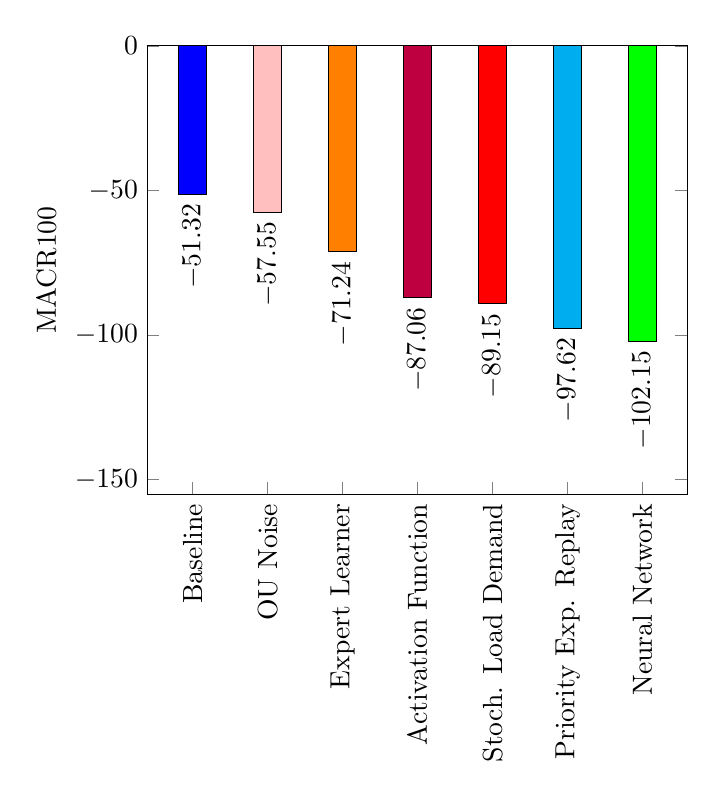
\begin{tikzpicture}
	\begin{axis}[
	    ylabel={MACR100},
	    symbolic x coords={Baseline,, OU Noise,, Expert Learner,, Activation Function,, Stoch. Load Demand,, Priority Exp. Replay,, Neural Network},
	    xtick = {Baseline, Neural Network, Activation Function, OU Noise, Priority Exp. Replay, Expert Learner, Stoch. Load Demand},
	    xticklabel style={rotate=90},
	    nodes near coords,
	    nodes near coords align={vertical},
	    every node near coord/.append style={rotate=90, anchor=east},
	    ymin=-155, ymax=0
	    ]
	\addplot [ybar, fill=blue] coordinates {(Baseline, -51.32)};
	\addplot [ybar, fill=green] coordinates {(Neural Network, -102.15)};
	\addplot [ybar, fill=purple] coordinates {(Activation Function, -87.06)};
	\addplot [ybar, fill=pink] coordinates {(OU Noise, -57.55)};
	\addplot [ybar, fill=cyan] coordinates {(Priority Exp. Replay, -97.62)};
	\addplot [ybar, fill=orange] coordinates {(Expert Learner, -71.24)};
	\addplot [ybar, fill=red] coordinates {(Stoch. Load Demand, -89.15)};
	%\legend{Baseline, Neural Network, Activation Function, OU Noise, Priority Experience Replay, Expert Learner, Stochastic Load Demand};
	\end{axis}
\end{tikzpicture}}
		\caption{MACR100 at episode 10000.}\label{fig:7103_macr100_comparison}
	\end{minipage}
	\hspace{0.25cm}
	\begin{minipage}{0.50\textwidth}
		\resizebox{7cm}{!}{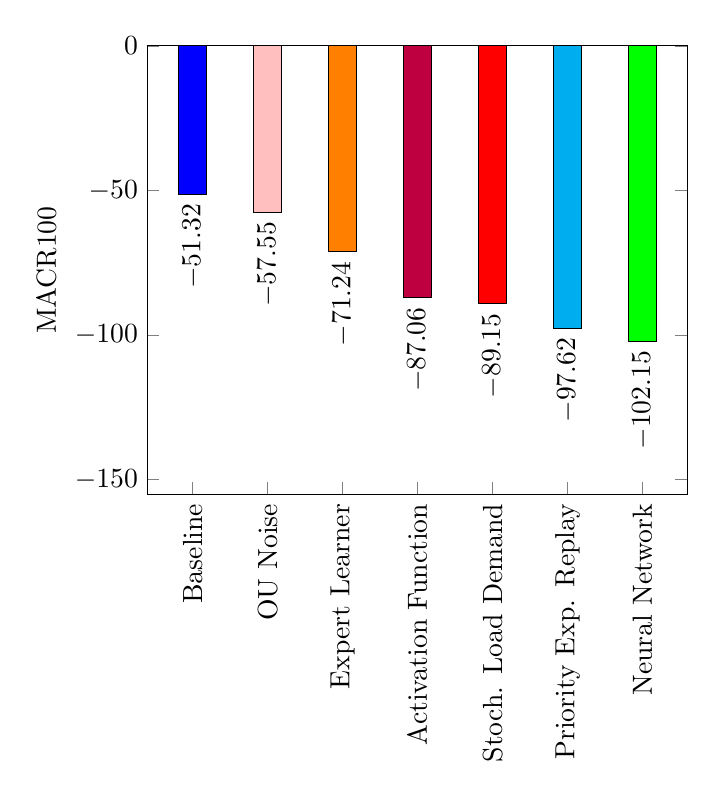
\begin{tikzpicture}
	\begin{axis}[
	    ylabel={MACR100},
	    symbolic x coords={Baseline,, OU Noise,, Expert Learner,, Activation Function,, Stoch. Load Demand,, Priority Exp. Replay,, Neural Network},
	    xtick = {Baseline, Neural Network, Activation Function, OU Noise, Priority Exp. Replay, Expert Learner, Stoch. Load Demand},
	    xticklabel style={rotate=90},
	    nodes near coords,
	    nodes near coords align={vertical},
	    every node near coord/.append style={rotate=90, anchor=east},
	    ymin=-155, ymax=0
	    ]
	\addplot [ybar, fill=blue] coordinates {(Baseline, -51.32)};
	\addplot [ybar, fill=green] coordinates {(Neural Network, -102.15)};
	\addplot [ybar, fill=purple] coordinates {(Activation Function, -87.06)};
	\addplot [ybar, fill=pink] coordinates {(OU Noise, -57.55)};
	\addplot [ybar, fill=cyan] coordinates {(Priority Exp. Replay, -97.62)};
	\addplot [ybar, fill=orange] coordinates {(Expert Learner, -71.24)};
	\addplot [ybar, fill=red] coordinates {(Stoch. Load Demand, -89.15)};
	%\legend{Baseline, Neural Network, Activation Function, OU Noise, Priority Experience Replay, Expert Learner, Stochastic Load Demand};
	\end{axis}
\end{tikzpicture}}
		\caption{Best MACR100 achieved during training.}\label{fig:7104_macr100_comparison}
	\end{minipage}
\end{figure}
 
\section{Trained Agent Performance}
The optimally tuned PI controller was able to perform the load frequency control task better than trained agents across all experiments. This was evident for most performance metrics. Despite agent performance being worse than the PI controller, trained agents were still able to arrest frequency deviations, providing an improvement over a system with no controller. The Baseline experiment demonstrated the best results for most performance metrics; however, the Baseline control policy caused system frequency oscillations, ultimately making it unusable. Control policies observed in the OU Noise and Stochastic Load Demand experiment also performed well. These agents exhibited more stable control characteristics when compared to the Baseline control policy; however, persistent frequency deviation offsets rendered them unusable. 

The remainder of this chapter discusses the trained agent performance with respect to each of the performance metrics.

\subsection{Cumulative Reward}
The optimally tuned PI controller received a better cumulative reward when compared to all experiments for both the +0.01pu and -0.01pu step change disturbances at the 5, 10, 15, 20, and 25 second marks. Figures \ref{fig:7201_cum_reward_pos} and \ref{fig:7202_cum_reward_neg} show the trained agent performance for for +0.01pu and -0.01pu step change disturbances at the 15 sec mark, respectively. The PI benchmark is included as a reference. For the +0.01pu step change disturbance the Baseline experiment performed the best with a cumulative reward marginally worse than the PI controller. The next best agent was the OU Noise experiment. For the -0.01pu step change disturbance the Priority Experience Replay experiment performed the best, closely followed by the Baseline. The worst performing agents were from the Activation Function and the Neural Network experiments.

It is clear that the trained agent cumulative reward performance displays inconsistency across positive and negative step change disturbances. This is evident in both the mismatching of cumulative rewards for +0.01pu and -0.01pu step disturbance scenarios, and also the performance ordering mismatch. This is in contrast to the PI controller, which maintains a consistent cumulative reward for the 15 sec mark in both positive and negative step change disturbance scenarios.
\begin{figure}[h]
	\begin{minipage}[t]{0.50\textwidth}
		\centering
		\resizebox{7cm}{!}{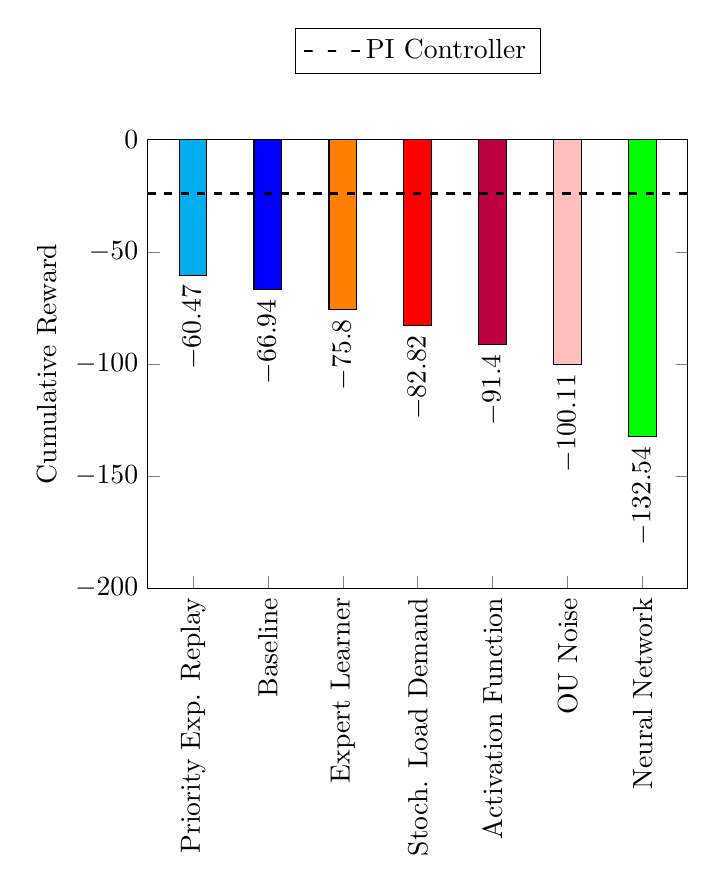
\begin{tikzpicture}
	\begin{axis}[
	    ylabel={Cumulative Reward},
	    symbolic x coords={Priority Exp. Replay,, Baseline,, Expert Learner,, Stoch. Load Demand,, Activation Function,, OU Noise,, Neural Network},
	    xtick = {Baseline, Neural Network, Activation Function, OU Noise, Priority Exp. Replay, Expert Learner, Stoch. Load Demand},
	    xticklabel style={rotate=90},
	    nodes near coords,
	    nodes near coords align={vertical},
	    every node near coord/.append style={rotate=90, anchor=east},
	    ymin=-200, ymax=0,
	    legend style={at={(0.5,1.25)},anchor=north}
	    ]
	\addplot [ybar, fill=blue] coordinates {(Baseline, -66.94)};
	\addplot [ybar, fill=green] coordinates {(Neural Network, -132.54)};
	\addplot [ybar, fill=purple] coordinates {(Activation Function, -91.40)};
	\addplot [ybar, fill=pink] coordinates {(OU Noise, -100.11)};
	\addplot [ybar, fill=cyan] coordinates {(Priority Exp. Replay, -60.47)};
	\addplot [ybar, fill=orange] coordinates {(Expert Learner, -75.80)};
	\addplot [ybar, fill=red] coordinates {(Stoch. Load Demand, -82.82)};
	%\legend{Baseline, Neural Network, Activation Function, OU Noise, Priority Experience Replay, Expert Learner, Stochastic Load Demand};
	\addplot[thick, black,dashed,sharp plot,nodes near coords={},update limits=false,shorten >=-10mm,shorten <=-10mm] 
			coordinates {(Priority Exp. Replay,-23.99) (Neural Network,-23.99)};
	\addlegendentry{PI Controller};
	\end{axis}
\end{tikzpicture}}
		\caption{Trained agent cumulative reward for a +0.01pu step change disturbance at the 15 sec mark.}\label{fig:7201_cum_reward_pos}
	\end{minipage}
	\hspace{0.25cm}
	\begin{minipage}[t]{0.50\textwidth}
		\resizebox{7cm}{!}{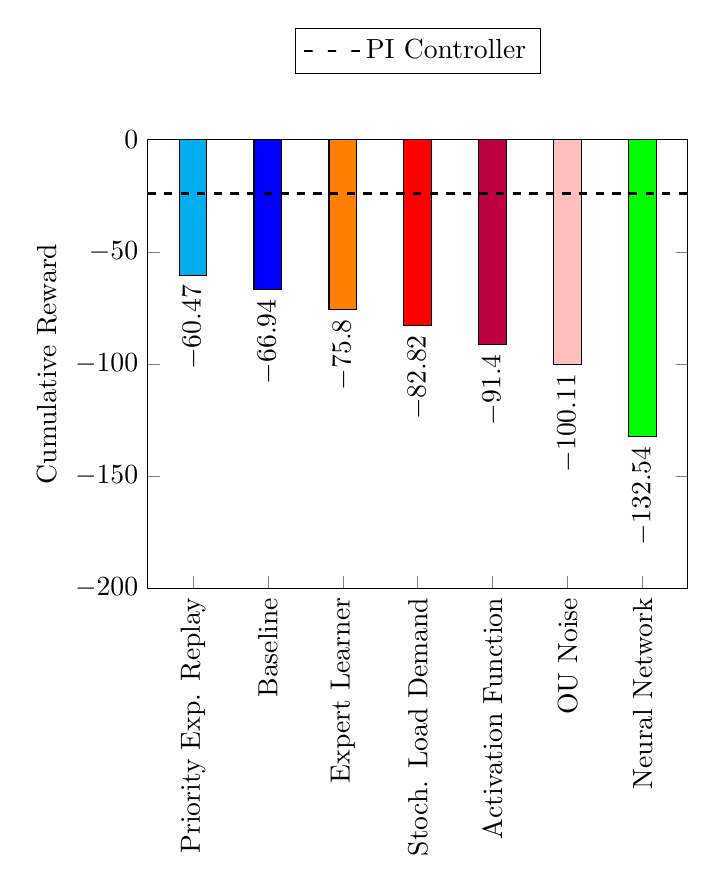
\begin{tikzpicture}
	\begin{axis}[
	    ylabel={Cumulative Reward},
	    symbolic x coords={Priority Exp. Replay,, Baseline,, Expert Learner,, Stoch. Load Demand,, Activation Function,, OU Noise,, Neural Network},
	    xtick = {Baseline, Neural Network, Activation Function, OU Noise, Priority Exp. Replay, Expert Learner, Stoch. Load Demand},
	    xticklabel style={rotate=90},
	    nodes near coords,
	    nodes near coords align={vertical},
	    every node near coord/.append style={rotate=90, anchor=east},
	    ymin=-200, ymax=0,
	    legend style={at={(0.5,1.25)},anchor=north}
	    ]
	\addplot [ybar, fill=blue] coordinates {(Baseline, -66.94)};
	\addplot [ybar, fill=green] coordinates {(Neural Network, -132.54)};
	\addplot [ybar, fill=purple] coordinates {(Activation Function, -91.40)};
	\addplot [ybar, fill=pink] coordinates {(OU Noise, -100.11)};
	\addplot [ybar, fill=cyan] coordinates {(Priority Exp. Replay, -60.47)};
	\addplot [ybar, fill=orange] coordinates {(Expert Learner, -75.80)};
	\addplot [ybar, fill=red] coordinates {(Stoch. Load Demand, -82.82)};
	%\legend{Baseline, Neural Network, Activation Function, OU Noise, Priority Experience Replay, Expert Learner, Stochastic Load Demand};
	\addplot[thick, black,dashed,sharp plot,nodes near coords={},update limits=false,shorten >=-10mm,shorten <=-10mm] 
			coordinates {(Priority Exp. Replay,-23.99) (Neural Network,-23.99)};
	\addlegendentry{PI Controller};
	\end{axis}
\end{tikzpicture}}
		\caption{Trained agent cumulative reward for a -0.01pu step change disturbance at the 15 sec mark.}\label{fig:7202_cum_reward_neg}
	\end{minipage}
\end{figure}

\subsection{Frequency Deviations}
The optimally tuned PI controller demonstrated better performance, maintaining lower average absolute frequency deviations in Areas 1 and 2 when compared to all experiments for both +0.01pu and -0.01pu step change disturbances at the 5, 10, 15, 20, and 25 sec marks. Baseline and OU Noise experiments were able to show smaller maximum frequency deviations when compared to the PI controller in some instances. Figure \ref{fig:7203_max_freq} shows a comparison of the maximum frequency deviation of  the trained agents for a +0.01pu step change disturbance at the 15 sec mark, and Figure \ref{fig:7204_avg_freq} shows a comparison of the average frequency deviation for the same scenario. Both figures include the PI benchmark for comparison. The worst performing experiment for both average and maximum frequency deviation was the Activation Function.

Despite the Baseline experiment having the best recorded performance, visual inspection of the frequency signal for Areas 1 and 2 show undesirable oscillations occurring after the step change disturbance, resulting in an unusable policy for load frequency control. Oscillations such as these would cause unnecessary wear on generation units, and contribute to instability in the power system. Prior to the step change disturbance the controller was able to demonstrate similar levels of frequency stability seen in the PI controller. Frequency control plots for the Baseline experiment are shown in Figures \ref{fig:6202_freq_1} and \ref{fig:6204_freq_2}.

\begin{figure}[h]
	\begin{minipage}[t]{0.50\textwidth}
		\centering
		\resizebox{7cm}{!}{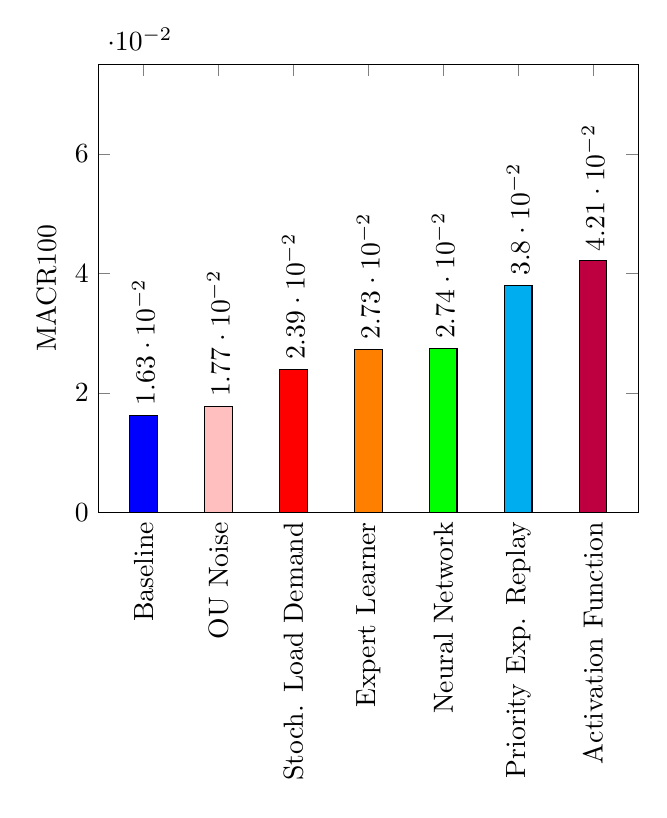
\begin{tikzpicture}
	\begin{axis}[
	    ylabel={MACR100},
	    symbolic x coords={Baseline,, OU Noise,, Stoch. Load Demand,, Expert Learner,, Neural Network,, Priority Exp. Replay,, Activation Function},
	    xtick = {Baseline, Neural Network, Activation Function, OU Noise, Priority Exp. Replay, Expert Learner, Stoch. Load Demand},
	    xticklabel style={rotate=90},
	    nodes near coords,
	    nodes near coords align={vertical},
	    every node near coord/.append style={rotate=90, anchor=west},
	    ymin=0, ymax=0.075
	    ]
	\addplot [ybar, fill=blue] coordinates {(Baseline, 0.0163)};
	\addplot [ybar, fill=green] coordinates {(Neural Network, 0.0274)};
	\addplot [ybar, fill=purple] coordinates {(Activation Function, 0.0421)};
	\addplot [ybar, fill=pink] coordinates {(OU Noise, 0.0177)};
	\addplot [ybar, fill=cyan] coordinates {(Priority Exp. Replay, 0.0380)};
	\addplot [ybar, fill=orange] coordinates {(Expert Learner, 0.0273)};
	\addplot [ybar, fill=red] coordinates {(Stoch. Load Demand, 0.0239)};
	%\legend{Baseline, Neural Network, Activation Function, OU Noise, Priority Experience Replay, Expert Learner, Stochastic Load Demand};
	\end{axis}
\end{tikzpicture}}
		\caption{Maximum frequency deviation for the trained agent in Area 1 during the +0.01pu step change disturbance at the 15 sec mark.}\label{fig:7203_max_freq}
	\end{minipage}
	\hspace{0.25cm}
	\begin{minipage}[t]{0.50\textwidth}
		\resizebox{7cm}{!}{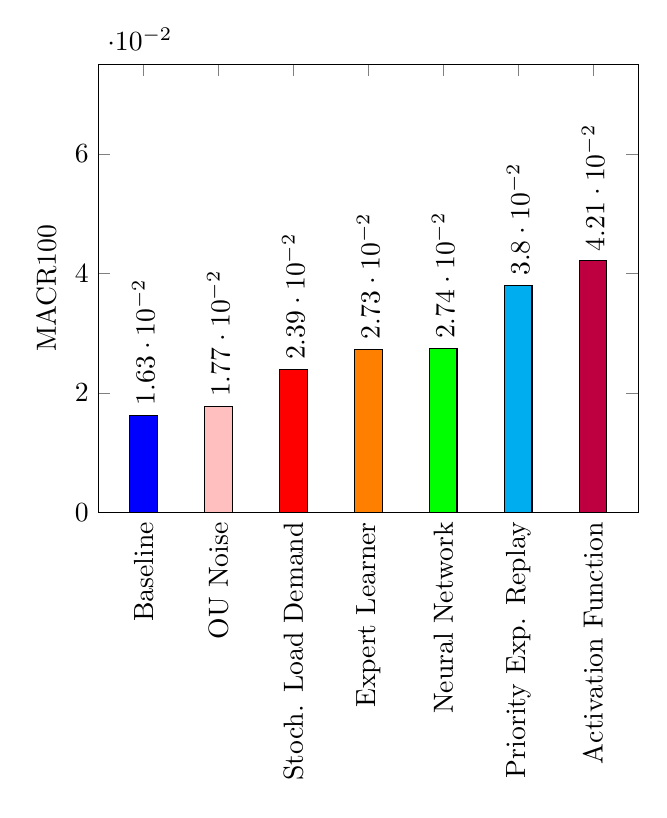
\begin{tikzpicture}
	\begin{axis}[
	    ylabel={MACR100},
	    symbolic x coords={Baseline,, OU Noise,, Stoch. Load Demand,, Expert Learner,, Neural Network,, Priority Exp. Replay,, Activation Function},
	    xtick = {Baseline, Neural Network, Activation Function, OU Noise, Priority Exp. Replay, Expert Learner, Stoch. Load Demand},
	    xticklabel style={rotate=90},
	    nodes near coords,
	    nodes near coords align={vertical},
	    every node near coord/.append style={rotate=90, anchor=west},
	    ymin=0, ymax=0.075
	    ]
	\addplot [ybar, fill=blue] coordinates {(Baseline, 0.0163)};
	\addplot [ybar, fill=green] coordinates {(Neural Network, 0.0274)};
	\addplot [ybar, fill=purple] coordinates {(Activation Function, 0.0421)};
	\addplot [ybar, fill=pink] coordinates {(OU Noise, 0.0177)};
	\addplot [ybar, fill=cyan] coordinates {(Priority Exp. Replay, 0.0380)};
	\addplot [ybar, fill=orange] coordinates {(Expert Learner, 0.0273)};
	\addplot [ybar, fill=red] coordinates {(Stoch. Load Demand, 0.0239)};
	%\legend{Baseline, Neural Network, Activation Function, OU Noise, Priority Experience Replay, Expert Learner, Stochastic Load Demand};
	\end{axis}
\end{tikzpicture}}
		\caption{Average frequency deviation for the trained agent in Area 1 during the +0.01pu step change disturbance at the 15 sec mark.}\label{fig:7204_avg_freq}
	\end{minipage}
\end{figure}

Increased frequency signal stability was observed for both OU Noise and Stochastic Load Demand experiments. Similarly to the Baseline controller, the OU Noise experiment maintained stability prior to the step change disturbance, although the Stochastic Load Demand experiment did not. Both agents were observed to dampen signal ringing; however, despite apparent frequency signal convergence, a zero level offset persisted. This implies OU Noise and Stochastic Load Demand agents, in their current state, are incapable of restoring frequency deviations after a disturbance. This makes them unsuitable for use as load frequency controllers. Frequency control plots for the OU Noise experiment are shown in Figures \ref{fig:6502_freq_1} and \ref{fig:6504_freq_2}. Frequency control plots for the Stochastic Load Demand experiment are shown in Figures \ref{fig:6802_freq_1} and \ref{fig:6804_freq_2}. It is worth highlighting that, but for the offsets, frequency signals are very similar to the tuned PI controller as indicated by the dotted lines.

\subsection{Control Effort}
The optimally tuned PI controller demonstrated a maximum absolute control effort that was equal to or less than that for all experiments for Areas 1 and 2. Despite this result, on average the PI controller used more control effort throughout the simulation. In particular, the OU Noise, Baseline, and Priority Experience Replay agents out performed the PI controller for this metric.

\begin{figure}[h]
	\begin{minipage}[t]{0.50\textwidth}
		\centering
		\resizebox{7cm}{!}{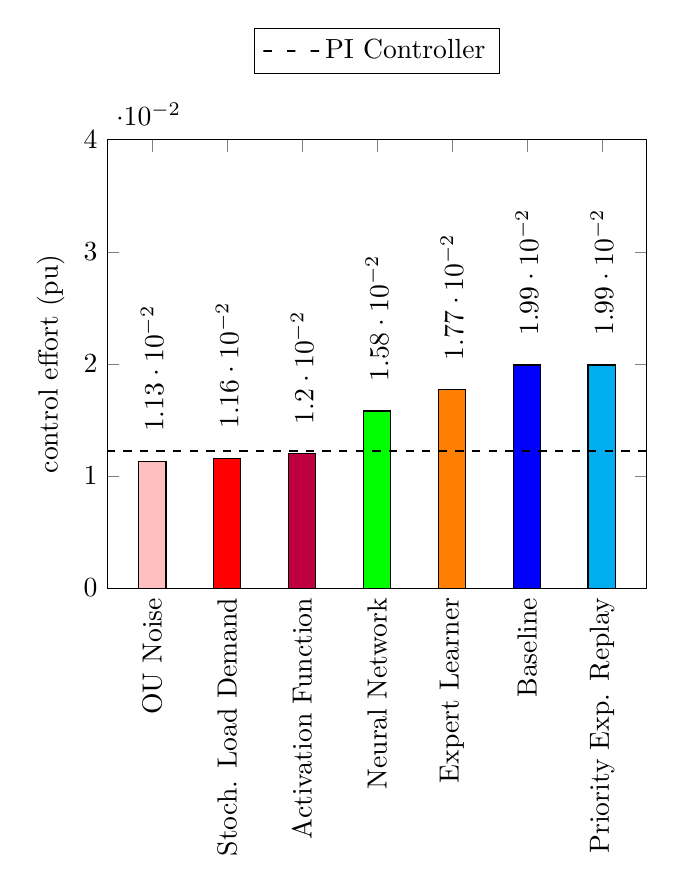
\begin{tikzpicture}
	\begin{axis}[
	    ylabel={control effort (pu)},
	    symbolic x coords={OU Noise,, Stoch. Load Demand,, Activation Function,, Neural Network,, Expert Learner,, Baseline,, Priority Exp. Replay},
	    xtick = {Baseline, Neural Network, Activation Function, OU Noise, Priority Exp. Replay, Expert Learner, Stoch. Load Demand},
	    xticklabel style={rotate=90},
	    nodes near coords,
	    nodes near coords align={vertical},
	    every node near coord/.append style={rotate=90, anchor=west, xshift=0.25cm},
	    ymin=0, ymax=0.04,
	    legend style={at={(0.5,1.25)},anchor=north}
	    ]
	\addplot [ybar, fill=blue] coordinates {(Baseline, 0.0199)};
	\addplot [ybar, fill=green] coordinates {(Neural Network, 0.0158)};
	\addplot [ybar, fill=purple] coordinates {(Activation Function, 0.012)};
	\addplot [ybar, fill=pink] coordinates {(OU Noise, 0.0113)};
	\addplot [ybar, fill=cyan] coordinates {(Priority Exp. Replay, 0.0199)};
	\addplot [ybar, fill=orange] coordinates {(Expert Learner, 0.0177)};
	\addplot [ybar, fill=red] coordinates {(Stoch. Load Demand, 0.0116)};
	%\legend{Baseline, Neural Network, Activation Function, OU Noise, Priority Experience Replay, Expert Learner, Stochastic Load Demand};
	\addplot[thick, black,dashed,sharp plot,nodes near coords={},update limits=false,shorten >=-10mm,shorten <=-10mm] 
			    coordinates {(OU Noise,0.0122) (Priority Exp. Replay,0.0122)};
	\addlegendentry{PI Controller};
	\end{axis}
\end{tikzpicture}}
		\caption{Maximum control effort for the trained agent in Area 1 during the +0.01pu step change disturbance at the 15 sec mark.}\label{fig:7205_max_ctl_effort}
	\end{minipage}
	\hspace{0.25cm}
	\begin{minipage}[t]{0.50\textwidth}
		\resizebox{7cm}{!}{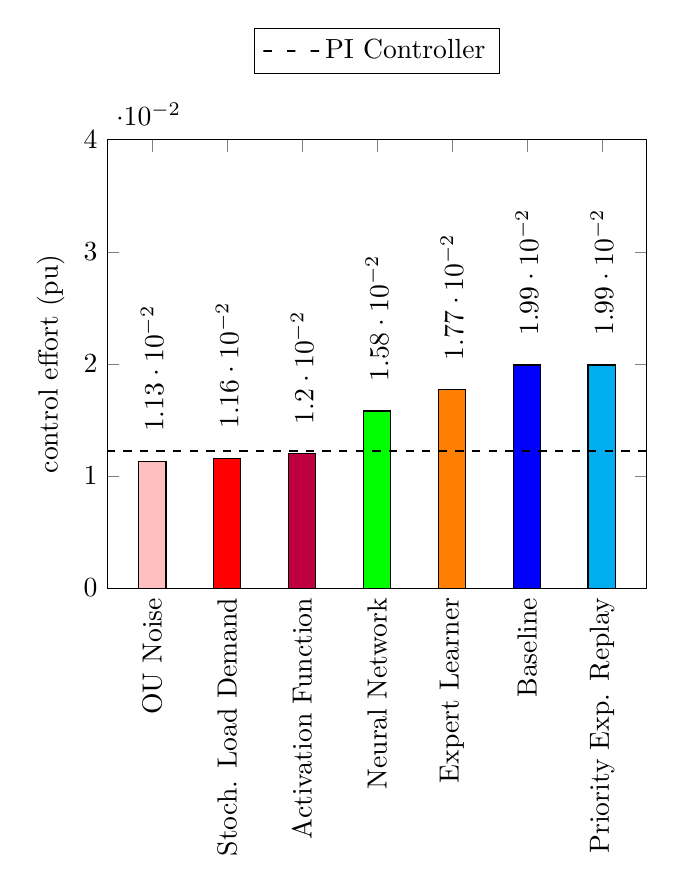
\begin{tikzpicture}
	\begin{axis}[
	    ylabel={control effort (pu)},
	    symbolic x coords={OU Noise,, Stoch. Load Demand,, Activation Function,, Neural Network,, Expert Learner,, Baseline,, Priority Exp. Replay},
	    xtick = {Baseline, Neural Network, Activation Function, OU Noise, Priority Exp. Replay, Expert Learner, Stoch. Load Demand},
	    xticklabel style={rotate=90},
	    nodes near coords,
	    nodes near coords align={vertical},
	    every node near coord/.append style={rotate=90, anchor=west, xshift=0.25cm},
	    ymin=0, ymax=0.04,
	    legend style={at={(0.5,1.25)},anchor=north}
	    ]
	\addplot [ybar, fill=blue] coordinates {(Baseline, 0.0199)};
	\addplot [ybar, fill=green] coordinates {(Neural Network, 0.0158)};
	\addplot [ybar, fill=purple] coordinates {(Activation Function, 0.012)};
	\addplot [ybar, fill=pink] coordinates {(OU Noise, 0.0113)};
	\addplot [ybar, fill=cyan] coordinates {(Priority Exp. Replay, 0.0199)};
	\addplot [ybar, fill=orange] coordinates {(Expert Learner, 0.0177)};
	\addplot [ybar, fill=red] coordinates {(Stoch. Load Demand, 0.0116)};
	%\legend{Baseline, Neural Network, Activation Function, OU Noise, Priority Experience Replay, Expert Learner, Stochastic Load Demand};
	\addplot[thick, black,dashed,sharp plot,nodes near coords={},update limits=false,shorten >=-10mm,shorten <=-10mm] 
			    coordinates {(OU Noise,0.0122) (Priority Exp. Replay,0.0122)};
	\addlegendentry{PI Controller};
	\end{axis}
\end{tikzpicture}}
		\caption{Average control effort for the trained agent in Area 1 during the +0.01pu step change disturbance at the 15 sec mark.}\label{fig:7205_avg_ctl_effort}
	\end{minipage}
\end{figure}

Figures \ref{fig:7205_max_ctl_effort} and \ref{fig:7205_avg_ctl_effort} show the maximum and average control effort for Area 1 given a +0.01pu step change disturbance at the 15 sec mark, respectively.

A visual inspection of the control signal for the OU Noise experiment highlights that the control signal is very similar to that of the optimally tuned PI controller. The principal difference between PI and OU Noise control signals are the Area 1 signal being too low, and the Area 2 signal being too high. Furthermore, there is a small deviation in the control signal prior to the disturbance which results in unnecessary frequency deviations. The control signals in Areas 1 and 2 for the OU Noise experiment given a +0.01pu step change disturbance at the 15 sec mark are shown in Figures \ref{fig:6503_ctl_1} and \ref{fig:6505_ctl_2}, respectively.

The similarity in the PI and Stochastic Load Demand control signals are even more pronounced. Notably, after the step change disturbance, the control signal tracks the PI control signal very closely. The principal different is prior to the step change disturbance where the Stochastic Load Demand control signal demonstrates some oscillatory behaviour resulting in unnecessary frequency disturbance. The control signals in Areas 1 and 2 for the Stochastic Load Demand experiment given a +0.01pu step change disturbance at the 15 sec mark are shown in Figures \ref{fig:6803_ctl_1} and \ref{fig:6805_ctl_2}, respectively.


\subsection{Settling Time}
The PI controller outperformed the Baseline, OU Noise, Activation Function, and Priority Experience Replay experiments for settling times under all scenarios for Areas 1 and 2.

\begin{figure}[h]
	\begin{minipage}[t]{0.50\textwidth}
		\centering
		\resizebox{7cm}{!}{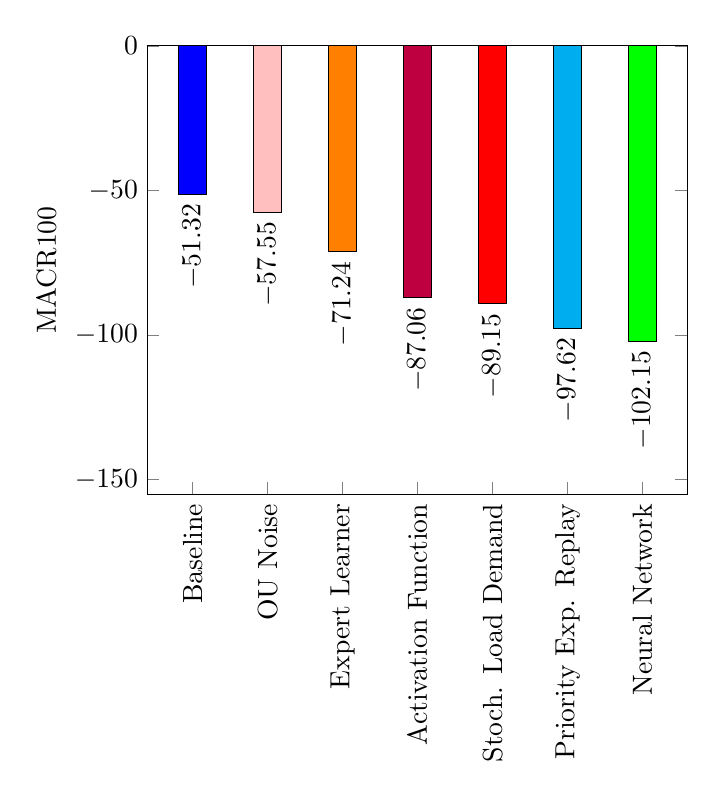
\begin{tikzpicture}
	\begin{axis}[
	    ylabel={MACR100},
	    symbolic x coords={Baseline,, OU Noise,, Expert Learner,, Activation Function,, Stoch. Load Demand,, Priority Exp. Replay,, Neural Network},
	    xtick = {Baseline, Neural Network, Activation Function, OU Noise, Priority Exp. Replay, Expert Learner, Stoch. Load Demand},
	    xticklabel style={rotate=90},
	    nodes near coords,
	    nodes near coords align={vertical},
	    every node near coord/.append style={rotate=90, anchor=east},
	    ymin=-155, ymax=0
	    ]
	\addplot [ybar, fill=blue] coordinates {(Baseline, -51.32)};
	\addplot [ybar, fill=green] coordinates {(Neural Network, -102.15)};
	\addplot [ybar, fill=purple] coordinates {(Activation Function, -87.06)};
	\addplot [ybar, fill=pink] coordinates {(OU Noise, -57.55)};
	\addplot [ybar, fill=cyan] coordinates {(Priority Exp. Replay, -97.62)};
	\addplot [ybar, fill=orange] coordinates {(Expert Learner, -71.24)};
	\addplot [ybar, fill=red] coordinates {(Stoch. Load Demand, -89.15)};
	%\legend{Baseline, Neural Network, Activation Function, OU Noise, Priority Experience Replay, Expert Learner, Stochastic Load Demand};
	\end{axis}
\end{tikzpicture}}
		\caption{Trained agent settling time in Area 1 for the +0.01pu step change disturbance at the 15 sec mark.}\label{fig:7207_settling_time_area_1}
	\end{minipage}
	\hspace{0.25cm}
	\begin{minipage}[t]{0.50\textwidth}
		\resizebox{7cm}{!}{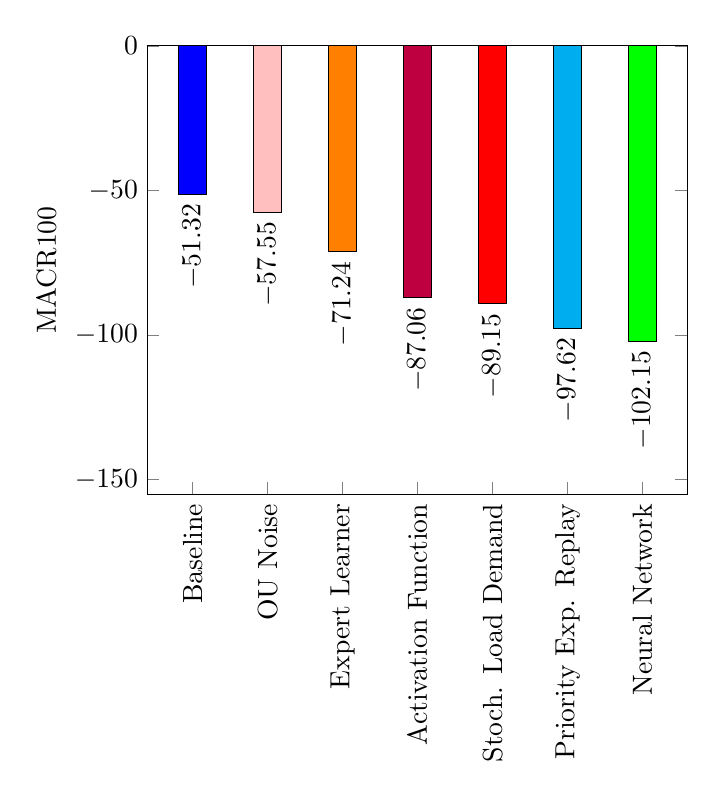
\begin{tikzpicture}
	\begin{axis}[
	    ylabel={MACR100},
	    symbolic x coords={Baseline,, OU Noise,, Expert Learner,, Activation Function,, Stoch. Load Demand,, Priority Exp. Replay,, Neural Network},
	    xtick = {Baseline, Neural Network, Activation Function, OU Noise, Priority Exp. Replay, Expert Learner, Stoch. Load Demand},
	    xticklabel style={rotate=90},
	    nodes near coords,
	    nodes near coords align={vertical},
	    every node near coord/.append style={rotate=90, anchor=east},
	    ymin=-155, ymax=0
	    ]
	\addplot [ybar, fill=blue] coordinates {(Baseline, -51.32)};
	\addplot [ybar, fill=green] coordinates {(Neural Network, -102.15)};
	\addplot [ybar, fill=purple] coordinates {(Activation Function, -87.06)};
	\addplot [ybar, fill=pink] coordinates {(OU Noise, -57.55)};
	\addplot [ybar, fill=cyan] coordinates {(Priority Exp. Replay, -97.62)};
	\addplot [ybar, fill=orange] coordinates {(Expert Learner, -71.24)};
	\addplot [ybar, fill=red] coordinates {(Stoch. Load Demand, -89.15)};
	%\legend{Baseline, Neural Network, Activation Function, OU Noise, Priority Experience Replay, Expert Learner, Stochastic Load Demand};
	\end{axis}
\end{tikzpicture}}
		\caption{Trained agent settling time in Area 2 for the +0.01pu step change disturbance at the 15 sec mark.}\label{fig:7208_settling_time_area_2}
	\end{minipage}
\end{figure}

For selected scenarios the Expert Learner, and Neural Network experiments were able to obtain better settling times that the PI Controller. The Stochastic Load Demand experiment outperformed the PI controller under all cases.

The Baseline, OU Noise, Activation Function, and Priority Experience Replay experiments were not able to develop control policies that dampened frequency signals sufficiently to qualify for the settling time definition outlined in \textsection \ref{sec:agent_performance}. This meant that a settling time could not be obtained for these agents. The Stochastic Load Demand agent, and to a lesser degree Expert Learner and Neural Network agents, were often able to demonstrate settling times that were half that of the PI controller.

Figures \ref{fig:7207_settling_time_area_1} and \ref{fig:7208_settling_time_area_2} show the settling times for Areas 1 and 2 given a +0.01pu step change disturbance 
